\documentclass[9pt,letter,twoside,openright,fleqn]{memoir}
\usepackage[svgnames,table]{xcolor}
\usepackage{circuitikz}
\usepackage{xparse}
\usepackage{filecontents}
%\usepackage{minibox}
\usepackage{longtable}
\usepackage{amsmath,pgfplots}
\usepgfplotslibrary{statistics}
\usepackage[shortlabels]{enumitem}
%\usepackage{tkz-euclide}
%\usetkzobj{all}

\usepackage{tikz}
\usepackage{tkz-berge}

\usetikzlibrary{decorations.fractals,calc,decorations.markings}
\usetikzlibrary{arrows,decorations.markings,positioning}
\newcommand{\tikzmark}[2]{\tikz[overlay, remember picture] \node[inner sep=5pt, outer sep=5pt, anchor=base] (#1) {#2};}

\usepackage{amssymb}
\usepackage{etoolbox}
\usepackage{cancel}
\usepackage{array}
\usepackage{graphicx}
\usepackage{framed}
\usepackage{tcolorbox}
\tcbuselibrary{breakable,skins,xparse}
\usepackage{marginnote}
%\usepackage{verbatim}
\usepackage[style=2]{mdframed}
\usepackage[top=0.75in, bottom=0.75in, inner=0.75in, outer=2.5in, marginparwidth=1.75in, marginparsep=0.25in]{geometry}
\usepackage{titlesec}
\usepackage[official]{eurosym}
%\usepackage[Bjornstrup]{fncychap}

\usepackage{changepage}
\usepackage[T1]{fontenc}
\usepackage{lmodern}
%\usepackage{url}
\usepackage{comment}
\ifpdf
  \usepackage{pdfcolmk}
\fi
\usepackage{graphicx}
\usepackage[hidelinks]{hyperref}
%\usepackage[outline]{contour}
\usepackage{pifont}
%\ifxetex
%  \usepackage{fontspec}
%\fi

\strictpagecheck
\addtocontents{toc}{\protect\thispagestyle{empty}}

%%%%Author Name in Table of Contents---------
\makeatletter
\let\@nodottedtocline\@dottedtocline
\patchcmd{\@nodottedtocline}{\hbox{.}}{\hbox{}}{}{}
\patchcmd{\@nodottedtocline}{\normalcolor #5}{\normalcolor}{}{}
\newcommand*\l@sectionsubtitle{\@nodottedtocline{1}{0em}{1.5em}}
\makeatother

\def\sectionsubtitle#1{%
    \addcontentsline{toc}{sectionsubtitle}{\protect\numberline{}\textit{#1}}%
}
%%%%------------------------------------------

%%%%Define Gaussian Plot for Stats Chapter
\pgfmathdeclarefunction{gauss}{2}{%
  \pgfmathparse{1/(#2*sqrt(2*pi))*exp(-((x-#1)^2)/(2*#2^2))}%
}
%%%%End Define Gaussian Plot

%%%%Drawing Fractal
\newcommand{\bedknobsthree}[1]{
    %\begin{center}
        \tikz [
            decoration = #1
        ] \draw decorate{ decorate{ decorate{ (0, 0) -- (0.35\linewidth, 0) }}};
    %\end{center}
}
%%%%Drawing Fractal

%%%%Begin Header Format
\nouppercaseheads
\copypagestyle{doc}{companion}
\makeevenhead{doc}{\textbf{\Large \thepage} \hspace{0.1in} \textbf{CHAPTER \thechapter} \hspace{0.1in} \leftmark}{}{}
\makeoddhead{doc}{}{}{SECTION \rightmark \hspace{0.1in} \textbf{\Large \thepage}}
\makeevenfoot{doc}{}{}{}
\makeoddfoot{doc}{}{}{}
\makeheadrule{doc}{\textwidth}{0pt} %Uncomment to remove headrule

\copypagestyle{algebra}{doc}
\makeevenhead{algebra}{\textbf{\Large \thepage} \hspace{0.1in} \textbf{CHAPTER R \hspace{0.1in} \leftmark}}{}{}

\copypagestyle{chapter}{doc}
\makeevenhead{chapter}{}{}{}
\makeoddhead{chapter}{}{}{}
\makeevenfoot{chapter}{\textbf{\Large \thepage}}{}{}
\makeoddfoot{chapter}{\hfill}{\hfill}{\textbf{\Large \thepage}}
\makeheadrule{chapter}{\textwidth}{0pt} %Uncomment to remove headrule

\copypagestyle{exercise}{doc}
\makeevenfoot{exercise}{
\begin{tikzpicture}[overlay,remember picture]
      \fill [color=blue!60!black]
        ($ (current page.north west) - (1cm,-1cm) $)
        rectangle
        ($ (current page.south west) + (1cm,-1cm) $);
\end{tikzpicture}
}{}{}
\makeoddfoot{exercise}{\hfill}{\hfill}{
\begin{tikzpicture}[overlay,remember picture]
      \fill [color=blue!60!black]
        ($ (current page.north east) + (1cm,1cm) $)
        rectangle
        ($ (current page.south east) - (1cm,1cm) $);
\end{tikzpicture}
}

\setsecheadstyle{\Large\scshape\raggedright\bfseries\color{blue!30!black}}
\setsubsecheadstyle{\large\scshape\raggedright}
\setsubsubsecheadstyle{\normalsize\scshape\raggedright}
\setbeforesecskip{-1.5ex plus -.5ex minus -.2ex}
\setaftersecskip{1.3ex plus .2ex}
\setbeforesubsecskip{-1.25ex plus -.5ex minus -.2ex}
\setaftersubsecskip{1ex plus .2ex}
%%%%End Header Format

%%%%Begin Chapter Header Format
\usepackage{color,calc}
\newsavebox{\ChpNumBox}
\definecolor{ChapBlue}{rgb}{0.2,0.6,1}
\makeatletter
%\newcommand*{\thickhrulefill}{%
%\leavevmode\leaders\hrule height 1\p@ \hfill \kern \z@}
\newcommand*{\thickhrulefill}{\rule{1.0\textwidth}{5pt}}
\newcommand*\BuildChpNum[2]{%
\begin{tabular}[t]{@{}c@{}}
\makebox[0pt][c]{#1\strut} \\[.5ex]
\colorbox{ChapBlue}{%
\rule[-10em]{0pt}{0pt}%
\rule{1ex}{0pt}\color{black}#2\strut
\rule{1ex}{0pt}}%
\end{tabular}}
\makechapterstyle{BlueBox}{%
\renewcommand{\chapnamefont}{\large\scshape}
\renewcommand{\chapnumfont}{\Huge\bfseries}
\renewcommand{\chaptitlefont}{\raggedright\Huge\bfseries}
\setlength{\beforechapskip}{20pt}
\setlength{\midchapskip}{26pt}
\setlength{\afterchapskip}{40pt}
\renewcommand{\printchaptername}{}
\renewcommand{\chapternamenum}{}
\renewcommand{\printchapternum}{%
\sbox{\ChpNumBox}{%
\BuildChpNum{\chapnamefont\@chapapp}%
{\chapnumfont\thechapter}}}
\renewcommand{\printchapternonum}{%
\sbox{\ChpNumBox}{%
\BuildChpNum{\chapnamefont\vphantom{\@chapapp}}%
{\chapnumfont\hphantom{\thechapter}}}}
\renewcommand{\afterchapternum}{}
\renewcommand{\printchaptertitle}[1]{%
\usebox{\ChpNumBox}\hfill
\parbox[t]{\hsize-\wd\ChpNumBox-1em}{%
\vspace{\midchapskip}%
\thickhrulefill\par
\chaptitlefont ##1\par}}%
}
\chapterstyle{BlueBox}
%%%%End Chapter Header Format

%%%%Begin Title Page Definition
\newlength{\drop}
\newcommand*{\FSfont}[1]{%
  \fontencoding{T1}\fontfamily{#1}\selectfont}
\renewcommand*{\FSfont}[1]{}%    kills special font selections

\newcommand*{\rotrt}[1]{\rotatebox{90}{#1}}
\newcommand*{\rotlft}[1]{\rotatebox{-90}{#1}}
\newcommand*{\topb}{%
  \resizebox*{\unitlength}{\baselineskip}{\rotrt{$\}$}}}
\newcommand*{\botb}{%
  \resizebox*{\unitlength}{\baselineskip}{\rotlft{$\}$}}}
\newcommand*{\titleBC}{\begingroup
\begin{center}
\settowidth{\unitlength}{\textit{\Large COMMON APPLICATIONS OF MATHEMATICS}} 
{\color{LightGoldenrod}\topb} \\[\baselineskip]
\textcolor{Sienna}{\textit{\HUGE Versatile Mathematics}} \\[\baselineskip]
{\color{RosyBrown}\Large COMMON MATHEMATICAL APPLICATIONS} \\
{\color{LightGoldenrod}\botb}
\end{center}
\vfill
\begin{center}
{\LARGE\textbf{Josiah Hartley}}\\ Frederick Community College\\ \text{}\\ \text{}\\
{\LARGE\textbf{Val Lochman}}\\ Frederick Community College\\ \text{}\\ \text{}\\
{\LARGE\textbf{Erum Marfani}}\\ Frederick Community College\\ \text{}\\ \text{}\\
\vfill
{\huge\textbf{2nd Edition}}\\ \text{}\\ \text{}\\
{\LARGE\textbf{2020}}
\end{center}
\endgroup}

\newcommand*{\titleSolutionManual}{\begingroup
\begin{center}
\settowidth{\unitlength}{\textit{\Large COMMON APPLICATIONS OF MATHEMATICS}} 
{\color{LightGoldenrod}\topb} \\[\baselineskip]
\textcolor{Sienna}{\textit{\HUGE Versatile Mathematics}} \\[\baselineskip]
{\color{RosyBrown}\Large COMMON MATHEMATICAL APPLICATIONS} \\
{\color{LightGoldenrod}\botb}
\end{center}
\vfill
\begin{center}
{\HUGE\textbf{Instructor Solution Manual}}\\ \text{}\\
{\LARGE\textbf{NOT FOR USE BY STUDENTS}}
\end{center}
\vfill
\begin{center}
{\LARGE\textbf{Josiah Hartley}}\\ Frederick Community College\\ \text{}\\ \text{}\\
{\LARGE\textbf{Val Lochman}}\\ Frederick Community College\\ \text{}\\ \text{}\\
{\LARGE\textbf{Erum Marfani}}\\ Frederick Community College\\ \text{}\\ \text{}\\
\vfill
{\huge\textbf{2nd Edition}}\\ \text{}\\ \text{}\\
{\LARGE\textbf{2020}}
\end{center}
\endgroup}
%%%%End Title Page Definition

%Makes labels on axes smaller
\pgfplotsset{
    every axis/.append style={font=\tiny},  
}
%

%%%%Begin Procedure Definition
\newtcolorbox{proc}[1]{enhanced,colback=green!5!white,colframe=green!40!white!40!black,drop fuzzy shadow, toprule=5pt,bottomrule=0mm,rightrule=0mm,leftrule=0mm,fonttitle=\large,title={\fontfamily{fvs}\selectfont \textbf{#1}},sharp corners=all}
%%%%End Procedure Definition

\def\fra#1#2{\vskip #2\noindent\textcolor{black!60!red}{\rule{\textwidth}{2pt}}}

%%%%Begin Try It Definition
\renewcommand{\pfbreakdisplay}{%
\ding{167}\quad\ding{167}\quad\ding{167}}

\newenvironment{try}[1][]
{
\begin{tcolorbox}[enhanced,beforeafter skip=10pt,breakable,colframe=yellow!10,colback=yellow!10,drop lifted shadow,sharp corners=all]
\marginnote{\href{#1}{\fontfamily{fvs}\selectfont \Large\color{black!70!orange}\textbf{TRY IT}}}
}
{ \end{tcolorbox}}

\newenvironment{trynolabel}[1][]
{
\begin{tcolorbox}[enhanced,beforeafter skip=10pt,breakable,colframe=yellow!10,colback=yellow!10,drop lifted shadow,sharp corners=all]
}
{ \end{tcolorbox}}
%%%%End Try It Definition

%%%%Begin Formula Definition
\newenvironment{formula}[1]
{\begin{tcolorbox}[beforeafter skip=10pt,colframe=black!10,colback=blue!70!cyan!20!white,opacityfill=0.5,toprule=0mm,bottomrule=0mm,rightrule=0mm,leftrule=0mm,sharp corners=all]

{\fontfamily{fvs}\selectfont \Large\bfseries #1}\\

}
{\end{tcolorbox}}
%%%%End Formula Definition

%%%%Counter for examples; reset for each chapter/section?
\newcounter{ExampleCounter}
\setcounter{ExampleCounter}{1}

%%%%Begin Example Definition
\begin{comment}
\newenvironment{example}[2][https://dl.dropboxusercontent.com/u/28928849/Webpages/MathInSocietyVideos2.htm]
{
\marginnote{\href{#1}{\fontfamily{fvs}\selectfont \Large\color{black!70!blue!80!cyan}\uppercase{\bfseries\centering EXAMPLE \theExampleCounter}
}}[9.2mm]
\begin{tcolorbox}[check odd page,toggle left and right,
beforeafter skip=10pt,breakable,bottomrule at break=0mm,toprule at break=0mm,colframe=black!50!blue!50!cyan,colback=white,toprule=0mm,rightrule=0mm,sharp corners=all] 
{%\renewcommand*\sfdefault{iwona}
\checkoddpage
\ifoddpage{
\hfill {\href{#1}{\fontfamily{fvs}\selectfont \Large\color{black!70!blue!80!cyan}\uppercase{\bfseries #2}}}}\\
 \else{
{\href{#1}{\fontfamily{fvs}\selectfont \Large\color{black!70!blue!80!cyan}\uppercase{\bfseries #2}}}}\\
\fi
\end{comment}

\colorlet{colexam}{black!50!blue!50!cyan}
\newenvironment{example}[2][]
{
\begin{tcolorbox}[empty,
breakable,
if odd page*={overlay unbroken={\coordinate (X) at ([yshift=-10pt]frame.north west); \coordinate (Y) at (frame.south west); \coordinate (Z) at (frame.south east);
\draw[black!50!blue!50!cyan,line width=2pt]
(X)--(Y)--(Z); },
overlay first={\coordinate (X) at ([yshift=-10pt]frame.north west); \coordinate (Y) at (frame.south west);
\draw[black!50!blue!50!cyan,line width=2pt]
(X)--(Y); },
overlay middle={\coordinate (X) at ([yshift=-10pt]frame.north west); \coordinate (Y) at (frame.south west);
\draw[black!50!blue!50!cyan,line width=2pt]
(X)--(Y); },
overlay last={\coordinate (X) at ([yshift=-10pt]frame.north west); \coordinate (Y) at (frame.south west); \coordinate (Z) at (frame.south east);
\draw[black!50!blue!50!cyan,line width=2pt]
(X)--(Y)--(Z); }}{overlay unbroken={\coordinate (X) at ([yshift=-10pt]frame.north east); \coordinate (Y) at (frame.south east); \coordinate (Z) at (frame.south west);
\draw[black!50!blue!50!cyan,line width=2pt]
(X)--(Y)--(Z); },
overlay first={\coordinate (X) at ([yshift=-10pt]frame.north east); \coordinate (Y) at (frame.south east);
\draw[black!50!blue!50!cyan,line width=2pt]
(X)--(Y); },
overlay middle={\coordinate (X) at ([yshift=-10pt]frame.north east); \coordinate (Y) at (frame.south east);
\draw[black!50!blue!50!cyan,line width=2pt]
(X)--(Y); },
overlay last={\coordinate (X) at ([yshift=-10pt]frame.north east); \coordinate (Y) at (frame.south east); \coordinate (Z) at (frame.south west);
\draw[black!50!blue!50!cyan,line width=2pt]
(X)--(Y)--(Z); }}] 
{%\renewcommand*\sfdefault{iwona}
\checkoddpage
\ifoddpage{
\hfill {\href{#1}{\fontfamily{fvs}\selectfont \Large\color{black!70!blue!80!cyan}\uppercase{\bfseries #2}\marginnote{\href{#1}{\fontfamily{fvs}\selectfont \Large\color{black!70!blue!80!cyan}\uppercase{\bfseries\centering EXAMPLE \theExampleCounter}
}}}}}\\
 \else{
{\href{#1}{\fontfamily{fvs}\selectfont \Large\color{black!70!blue!80!cyan}\uppercase{\bfseries #2}\marginnote{\href{#1}{\fontfamily{fvs}\selectfont \Large\color{black!70!blue!80!cyan}\uppercase{\bfseries\centering EXAMPLE \theExampleCounter}
}}}}}\\
\fi
%\renewcommand*\sfdefault{cmr}
}

%\Large\color{black!70!blue!80!cyan}\scshape #2}\\

}
{ \end{tcolorbox} \stepcounter{ExampleCounter}}

\newcommand{\sol}{
\begin{center}\textcolor{black!50!blue!50!cyan}{\line(1,0){250}}\end{center}
\marginnote{\bfseries Solution}
}
\newcommand{\solline}{
\begin{center}\textcolor{black!50!blue!50!cyan}{\line(1,0){250}}\end{center}
}
%%%%End Example Definition

\newcommand\calcbutton[1]{$\boxed{\textrm{#1}}$}
\newcommand\boxtext[1]{$\boxed{\textrm{#1}}$}

%%%%Begin Section Definition
\newcounter{SectionNo}[chapter]

\DeclareDocumentCommand \section { m }
{
\phantomsection
\stepcounter{section}
\addcontentsline{toc}{section}{\thesection\ #1}
\sectionmark{#1}

\checkoddpage
\ifoddpage{\begin{adjustwidth}{0in}{-1.75in}
\stepcounter{SectionNo}
	
	\tcbset{enhanced,colback=brown!70!white,colframe=brown!75!black}
	\begin{tcolorbox}[toprule=3mm,sharp corners = all]
	{\fontfamily{fvs}\selectfont \huge\bfseries\color{white} SECTION \thechapter .\theSectionNo} \ {\fontfamily{fvs}\selectfont \LARGE\bfseries\color{black!80} #1}
	\end{tcolorbox}
	
 \end{adjustwidth}}
\else{\begin{adjustwidth}{-1.75in}{0in}
\stepcounter{SectionNo}
	
	\tcbset{enhanced,colback=brown!70!white,colframe=brown!75!black}
	\begin{tcolorbox}[toprule=3mm,sharp corners = all]
	{\fontfamily{fvs}\selectfont \huge\bfseries\color{white} SECTION \thechapter .\theSectionNo} \ {\fontfamily{fvs}\selectfont \LARGE\bfseries\color{black!80} #1}
	\end{tcolorbox}
	
 \end{adjustwidth}}
\fi
}

\DeclareDocumentCommand \subsection { m }
{
\vspace{0.2in}
{\fontfamily{fvs}\selectfont \LARGE\color{brown!65!black} \textbf{#1}}
\vspace{0.1in}\\
}
%%%%End Section Definition

%%%%Begin Example 2.0 Definition
\newcounter{example}[SectionNo]

\DeclareDocumentCommand \examplet { O{www.google.com} +m O{www.frederick.edu} +m }
{
\stepcounter{example}
\checkoddpage
\ifoddpage{\begin{adjustwidth}{0in}{-1.75in}
\begin{tcolorbox}[enhanced,breakable,drop lifted shadow,sharp corners=all,sidebyside,sidebyside align=top seam,title=\href{#1}{{\Large\bfseries\color{blue!40!black}EXAMPLE \theexample}} \hfill \href{#3}{{\Large\bfseries\color{green!40!black} TRY IT}},colframe=white,bottomrule=0mm,righthand width=2in,bicolor,colback=brown!15!white,colbacklower=yellow!10] #2 \tcblower #4
\end{tcolorbox}
\end{adjustwidth}}
\else{
\begin{adjustwidth}{-1.75in}{0in}
\begin{tcolorbox}[enhanced,breakable,drop lifted shadow,sharp corners=all,sidebyside,sidebyside align=top seam,title=\href{#1}{{\Large\bfseries\color{blue!40!black}EXAMPLE \theexample}} \hfill \href{#3}{{\Large\bfseries\color{green!40!black} TRY IT}},colframe=white,bottomrule=0mm,righthand width=2in,bicolor,colback=brown!15!white,colbacklower=yellow!10] #2 \tcblower #4
\end{tcolorbox}
\end{adjustwidth}}
\fi
}

\begin{comment}
\DeclareDocumentCommand \example { O{www.google.com} +m }
{
\stepcounter{example}
\checkoddpage
\ifoddpage{\begin{adjustwidth}{0in}{-1.75in}
\begin{tcolorbox}[enhanced,breakable,drop lifted shadow,sharp corners=all,title=\href{#1}{{\Large\bfseries\color{blue!40!black}EXAMPLE \theexample}},colframe=white,bottomrule=0mm,colback=brown!15!white] #2
\end{tcolorbox}
\end{adjustwidth}}
\else{
\begin{adjustwidth}{-1.75in}{0in}
\begin{tcolorbox}[enhanced,breakable,drop lifted shadow,sharp corners=all,title=\href{#1}{{\Large\bfseries\color{blue!40!black}EXAMPLE \theexample}},colframe=white,bottomrule=0mm,colback=brown!15!white] #2
\end{tcolorbox}
\end{adjustwidth}}
\fi
}
\end{comment}
%%%%End Example 2.0 Definition

%%%%Begin Objectives Definition
%\newenvironment{objectives}
%{\begin{adjustwidth}{-1.5in}{0in}\begin{minipage}{0.5\textwidth}}
%{\end{minipage}\end{adjustwidth}}
\newenvironment{objectives}
{\marginnote{\begin{enumerate}}
{\end{enumerate}}}
%%%%End Objectives Definition

%%%%Begin Exercises Definition
\newcounter{ProblemNumber}

\newcommand\pone[1]{ %One exercise per line
  \noindent
  \begin{minipage}[t]{\textwidth}
  \vspace{0.1in}
    {\large\bfseries\theProblemNumber .} #1
  \vspace{0.1in}
  \end{minipage}
  \stepcounter{ProblemNumber}
}

\newcommand\ptwo[1]{ %Two exercises per line
  \noindent
  \begin{minipage}[t]{0.48\textwidth}
  \vspace{0.1in}
    {\large\bfseries\theProblemNumber .} #1
  \vspace{0.1in}
  \end{minipage}
  \stepcounter{ProblemNumber}
}

\newcommand\pthree[1]{ %Three exercises per line
  \noindent
  \begin{minipage}[t]{0.31\textwidth}
  \vspace{0.1in}
    {\large\bfseries\theProblemNumber .} #1
  \vspace{0.1in}
  \end{minipage}
  \stepcounter{ProblemNumber}
}

\newcommand\pfour[1]{ %Four exercises per line
  \noindent
  \begin{minipage}[t]{0.228\textwidth}
  \vspace{0.15in}
    {\large\bfseries\theProblemNumber .} #1
  \vspace{0.15in}
  \end{minipage}
  \stepcounter{ProblemNumber}
}

\newenvironment{exercises}
{ 
	\newgeometry{margin=0.75in}	
	\pagestyle{exercise}
	\setcounter{ProblemNumber}{1}
	\noindent{\href{https://www.myopenmath.com/index.php}{\Huge\bfseries\color{blue!60!black} Exercises \thesection}}\\
	\checkoddpage
	\ifoddpage{{\color{blue!60!black} \rule{1.5\textwidth}{3pt}}} 
	\else{\begin{adjustwidth}{-0.8in}{0in}{\color{blue!60!black} \par\noindent\hspace{-0.25\textwidth}\rule{1.75\textwidth}{3pt}}\end{adjustwidth}} 
	\fi
	%{\color{blue!60!black} \rule{1.1\textwidth}{3pt}}
	

%\begin{comment}
%\tikz[remember picture,overlay] {%
%\draw [blue!60!black,line width=10mm]
%(current page.south east)
%rectangle
%(current page.north east)
%;}
%\end{comment}


}
{ \setcounter{ProblemNumber}{1}
  \restoregeometry
  \pagestyle{doc} }
%%%%End Exercises Definition

%%%%Begin Chapter Summary Definition
\newenvironment{summary}
{ 
	\newgeometry{margin=0.75in}	
	\pagestyle{exercise}
	\setcounter{ProblemNumber}{1}
	\noindent{\href{https://www.myopenmath.com/index.php}{\Huge\bfseries\color{blue!60!black} Exercises \thesection}}\\
	{\color{blue!60!black} \rule{1.1\textwidth}{3pt}}
	

%\begin{comment}
%\tikz[remember picture,overlay] {%
%\draw [blue!60!black,line width=10mm]
%(current page.south east)
%rectangle
%(current page.north east)
%;}
%\end{comment}


}
{ \setcounter{ProblemNumber}{1}
  \restoregeometry
  \pagestyle{doc} }

%%%%End Chapter Summary Definition

%%%% Graph Theory Vertex Label
\newcommand\extralabel[4][0mm]{\node[label={[label distance=#1]#3:#4}] at (#2){};}
% looks like \extralabel[distance(optional)]{node name}{angle}{label text}

% middle arrows on graphs
\tikzset{->-/.style={
 decoration={
   markings,
   mark=at position #1 with {\arrow{>}}
   },
   postaction={decorate}
  },
  ->-/.default=0.5 % set default value for arrow position
}

% circled numbers (or other text)
\newcommand*\circled[1]{\tikz[baseline=(char.base)]{
  \node[shape=circle,draw,inner sep=2pt] (char) {#1};}}
\graphicspath{ {./Images/} }

\begin{document}
\frontmatter
\newgeometry{margin=1.25in}
\pagestyle{empty}
\titleSolutionManual
\vfill
%\frontmatter

This solution manual was created to accompany \emph{Versatile Mathematics}, an OER textbook developed at Frederick Community College in Maryland.\\

The solutions are shown here solely for the benefit of instructors, and this manual should not be shared with students.
\pagebreak

%\newgeometry{margin=0.75in}
\textbf{This text is licensed under a Creative Commons Attribution-Share Alike 3.0 United States License.}\\

To view a copy of this license, visit \href{http://creativecommons.org/licenses/by-sa/3.0/us/}{http://creativecommons.org/licenses/by-sa/3.0/us/} or send a letter to Creative Commons, 171 Second Street, Suite 300, San Francisco, California, 94105, USA\\

You are \textbf{free}:\\
\hspace*{0.25in} \textbf{to Share} -- to copy, distribute, display, and perform the work\\
\hspace*{0.25in} \textbf{to Remix} -- to make derivative works\\

Under the following conditions:\\
\hspace*{0.25in} \textbf{Attribution.}  You must attribute the work in the manner specified by the author or licensor (but not in any way that suggests that they endorse you or your use of the work).\\
\hspace*{0.25in} \textbf{Share Alike.}  If you alter, transform, or build upon this work, you may distribute the resulting work only under the same, similar, or a compatible license.\\

With the understanding of the following:\\
\hspace*{0.25in} \textbf{Waiver.}  Any of the above conditions can be waived if you get permission from the copyright holder.\\
\hspace*{0.25in} \textbf{Other Rights.}  In no way are any of the following rights affected by the license:
\begin{itemize}
\item Your fair dealing or fair use rights
\item Apart from the remix rights granted under this license, the authors' moral rights
\item Rights other persons may have either in the work itself or in how the work is used, such as publicity or privacy rights
\item Notice --- For any reuse or distribution, you must make clear to others the license terms of this work.  The best way to do this is with a link to the following web page: \href{http://creativecommons.org/licenses/by-sa/3.0/us/}{http://creativecommons.org/licenses/by-sa/3.0/us/}
\end{itemize}

\paragraph{Attributions} This book benefited tremendously from others who went before and freely shared their creative work.  The following is a short list of those whom we have to thank for their work and their generosity in contributing to the free and open sharing of knowledge.
\begin{itemize}
\item David Lippman, author of \textit{Math in Society}.  This book uses sections derived from his chapters on Finance, Growth Models, and Statistics.  He also administers MyOpenMath, the free online homework portal to which the problems in this text were added.
\item The developers of \href{onlinestatbook.com}{onlinestatbook.com}.
\item OpenStax College (their book \textit{Introductory Statistics} was used as a reference)

OpenStax College, \textit{Introductory Statistics}. OpenStax College. 19 September 2013. <http://cnx.org/content/col11562/latest/>
\item The authors of \href{https://www.openintro.org/stat/?stat_book=os}{OpenIntro Statistics}, which was also used as a reference.
\item The Saylor Foundation Statistics Textbook: http://www.saylor.org/site/textbooks/Introductory$\%$20Statistics.pdf
\end{itemize}

\paragraph{Thanks} The following is a short list of those whom we wish to thank for their help and support with this project.
\begin{itemize}
\item The President's office at Frederick Community College, for providing a grant to write the first chapters.
\item Gary Hull, who in his tenure as department chair gave us his full support and gave us the impetus to start the project, and generously shared his notes for MA 103.
\item The entire FCC math department, who provided untold support and encouragement, as well as aid in reviewing and editing the text.
\end{itemize}

%\restoregeometry





















%\clearpage
\setcounter{tocdepth}{1}
\newgeometry{margin=1.25in}
\tableofcontents*
\mainmatter
\restoregeometry
\pagestyle{doc}

\setlist[enumerate,1]{label=\bfseries\protect\circled{\arabic*}, ref=\arabic*}
\def\answer#1{\\ \text{} \hfill \textbf{Answer to \theenumi:} $\boxed{\textrm{#1}}$}
\def\answersub#1{\\ \text{} \hfill \textbf{Answer to \theenumi\theenumii:} $\boxed{\textrm{#1}}$}

\chapter{Financial Mathematics}
\vfill
\pagebreak

\setcounter{section}{1}
\setcounter{SectionNo}{1}
\section{Applied Percentage Problems}
\emph{For problems 1--8, convert each number to a percent.}
\begin{enumerate}
\item $\dfrac{1}{2}$ \answer{50\%}
\[\dfrac{1}{2} \times 100\% = 0.5 \times 100\% = 50\%\]

\item 0.04 \answer{4\%}
\[0.04 \times 100\% = 4\%\]

\item $\dfrac{3}{5}$ \answer{60\%}
\[\dfrac{3}{5} \times 100\% = 0.6 \times 100\% = 60\%\]

\item 0.79 \answer{79\%}
\[0.79 \times 100\% = 79\%\]

\item 1.35 \answer{135\%}
\[1.35 \times 100\% = 135\%\]

\item $\dfrac{10}{4}$ \answer{250\%}
\[\dfrac{10}{4} \times 100\% = 2.5 \times 100\% = 250\%\]

\item 12.5 \answer{1250\%}
\[12.5 \times 100\% = 1250\%\]

\item 0.0378 \answer{3.78\%}
\[0.0378 \times 100\% = 3.78\%\]
\end{enumerate}

\emph{For problems 9--16, convert each percent to a decimal.}
\begin{enumerate}
\setcounter{enumi}{8}
\item 33\% \answer{0.33}
\[33\% = \dfrac{33}{100} = 0.33\]

\item 2.6\% \answer{0.026}
\[2.6\% = \dfrac{2.6}{100} = 0.026\]

\item 124\% \answer{1.24}
\[124\% = \dfrac{124}{100} = 1.24\]

\item 1240.5\% \answer{12.405}
\[1240.5\% = \dfrac{1240.5}{100} = 12.405\]

\item 42\% \answer{0.42}
\[42\% = \dfrac{42}{100} = 0.42\]

\item 4.5\% \answer{0.045}
\[4.5\% = \dfrac{4.5}{100} = 0.045\]

\item 0.003\% \answer{0.00003}
\[0.003\% = \dfrac{0.003}{100} = 0.00003\]

\item $\dfrac{1}{4}\%$ \answer{0.0025}
\[\dfrac{1}{4}\% = 0.25\% = \dfrac{0.25}{100} = 0.0025\]

\item What is 12\% of 72? \answer{8.64}
\[x = (12\%)(72) = (0.12)(72) = 8.64\]

\item Ninety is what percentage of 200? \answer{45\%}
\[90 = (x)(200) \longrightarrow x = \dfrac{90}{200} = 0.45 = 45\%\]

\item Twenty is 15\% of what? \answer{133.33}
\[20 = (15\%)(x) \longrightarrow x = \dfrac{20}{15\%} = \dfrac{20}{0.15} = 133.33\]

\item Six is what percentage of 40? \answer{15\%}
\[6 = (x)(40) \longrightarrow x = \dfrac{6}{40} = 0.15 = 15\%\]

\item Forty is 91\% of what? \answer{43.96}
\[40 = (91\%)(x) \longrightarrow x = \dfrac{40}{91\%} = \dfrac{40}{0.91} = 43.96\]

\item What is 65\% of 65? \answer{42.25}
\[x = (65\%)(65) = (0.65)(65) = 42.25\]

\item In the fall of 2009 FCC enrolled 6,233 students.  Of those enrolled, 2,810 are in the 18-21 age group.  What percent of FCC students does this represent? \answer{45.1\%}
\[\dfrac{2810}{6233} = 0.451 = 45.1\%\]

\item Patrick left an \$8 tip on a \$50 restaurant bill.  What percent tip is that? \answer{16\%}
\[\dfrac{8}{50} = 0.16 = 16\%\]

\item Ireland has a 23\% VAT (value-added tax, similar to a sales tax).  How much will the VAT be on a purchase of a \euro 250 item? \answer{\euro 57.50}
\[(23\%)(250) = (0.23)(250) = 57.5\]

\item Employees in 2012 paid 4.2\% of their gross wages towards social security (FICA tax).  How much would someone earning \$45,000 a year pay toward social security? \answer{\$1890}
\[(4.2\%)(45,000) = (0.042)(45,000) = 1890\]

\item A project on Kickstarter was aiming to raise \$15,000 for a precision coffee press.  They ended up with 714 supporters, raising 557\% of their goal.  How much did they raise? \answer{\$83,550}
\[(557\%)(15,000) = (5.57)(15,000) = 83,550\]

\item Another Kickstarter project for an iPad stylus raised 1,253\% of their goal, finishing with a total of \$313,250 from 7,511 supporters.  What was their original goal? \answer{\$25,000}
\[(1253\%)(x) = 313,250 \longrightarrow x = \dfrac{313,250}{1253\%} = \dfrac{313,250}{12.53} = 25,000\]

\item One year ago the median price for a home was \$275,000.  Now the current median price for a home is \$235,000.  What was the percent decrease in the median price of a home over the last year? \answer{14.55\%}
\[275,000 - 235,000 = 40,000 \longrightarrow \dfrac{40,000}{275,000} = 0.1455 = 14.55\%\]

\item There were 943 tornadoes reported in the U.S. in 2013, and 897 tornadoes were reported in 2014.  What percent decrease was there from 2013 to 2014? \answer{4.88\%}
\[943 - 897 = 46 \longrightarrow \dfrac{46}{943} = 0.0488 = 4.88\%\]

\item The population of a town increased from 3,250 in 2008 to 4,300 in 2010.  Find the absolute and percent increase. \answer{absolute: 1050; percent: 32.3\%}
\begin{center}
Absolute: $4300 - 3250 = 1050$\\
Percent: $\dfrac{1050}{3250} = 0.323 = 32.3\%$
\end{center}

\item The number of CDs sold in 2010 was 114 million, down from 147 million the previous year.  Find the absolute and percent decrease. \answer{absolute: 33 million; percent: 22.45\%}
\begin{center}
Absolute: $147 - 114 = 33$\\
Percent: $\dfrac{33}{147} = 0.2245 = 22.45\%$
\end{center}

\item A company wants to decrease their energy use by 15\%.
\begin{enumerate}[(a)]
\item If their electric bill is currently \$2,200 a month, what will their bill be if they're successful? \answersub{\$1870}
\[(2200)(85\%) = (2200)(0.85) = 1870\]

\item If their next bill is \$1,700 a month, were they successful?  What percent decrease was there from the current bill? \answersub{Yes; 22.73\%}
\[2200 - 1700 = 500 \longrightarrow \dfrac{500}{2200} = 0.2273 = 22.73\%\]
\end{enumerate}

\item A store is hoping an advertising campaign will increase their number of customers by 30\%.  They currently have about 80 customers per day.
\begin{enumerate}[(a)]
\item How many customers will they have if their campaign is successful? \answersub{104}
\[(80)(130\%) = (80)(1.3) = 104\]

\item If they increase to 120 customers a day, were they successful?  What percent increase is this from the current level? \answersub{Yes; 50\%}
\[120 - 80 = 40 \longrightarrow \dfrac{40}{80} = 0.5 = 50\%\]
\end{enumerate}

\item An article reports that ``attendance dropped 6\% this year, to 300.''  What was the attendance before the drop? \answer{319}
\[(x)(94\%) = 300 \longrightarrow x = \dfrac{300}{94\%} = \dfrac{300}{0.94} \approx 319\]

\item An article reports that ``sales have grown by 30\% this year, to \$200 million.''  What were sales before the growth? \answer{153.85 million}
\[(x)(130\%) = 200 \longrightarrow x = \dfrac{200}{130\%} = \dfrac{200}{1.3} = 153.85\]

\item The U.S. federal debt at the end of 2001 was \$5.77 trillion, and grew to \$6.20 trillion by the end of 2002. At the end of 2005 it was \$7.91 trillion, and grew to \$8.45 trillion by the end of 2006. Calculate the absolute and relative increase for 2001-2002 and 2005-2006. Which year saw a larger relative increase in federal debt? \answer{0.43 trillion; 7.45\%; 0.54 trillion; 6.83\%; 2001-2002}
\begin{center}
2001-2002 (absolute): $6.20 - 5.77 = 0.43$ trillion\\
2001-2002 (relative): $\dfrac{0.43}{5.77} = 0.0745 = 7.45\%$\\ \text{}\\
2005-2006 (absolute): $8.45 - 7.91 = 0.54$ trillion\\
2005-2006 (relative): $\dfrac{0.54}{7.91} = 0.0683 = 6.83\%$
\end{center}

\item A TV originally priced at \$799 is on sale for 30\% off. There is then a 9.2\% sales tax. Find the price after including the discount and sales tax. \answer{\$610.76}
\[(799)(0.7) = 559.30 \longrightarrow (559.30)(1.092) = 610.76\]

\item The Walden University had 47,456 students in 2010, while Kaplan University had 77,966 students.  Complete the following statements.
\begin{enumerate}[(a)]
\item Kaplan's enrollment was \line(1,0){20} \% larger than Walden's. \answersub{64.29\%}
\[77,966 - 47,456 = 30,510 \longrightarrow \dfrac{30,510}{47,456} = 0.6429 = 64.29\%\]

\item Walden's enrollment was \line(1,0){20} \% smaller than Kaplan's. \answersub{39.13\%}
\[77,966 - 47,456 = 30,510 \longrightarrow \dfrac{30,510}{77,966} = 0.3913 = 39.13\%\]

\item Walden's enrollment was \line(1,0){20} \% of Kaplan's. \answersub{60.87\%}
\[\dfrac{47,456}{77,966} = 0.6087 = 60.87\%\]
\end{enumerate}

\item In the 2012 Olympics, Usain Bolt ran the 100 m dash in 9.63 seconds.  Jim Hines won the 1968 gold with a time of 9.95 seconds.
\begin{enumerate}[(a)]
\item Bolt's time was \line(1,0){20} \% faster than Hines'. \answersub{3.22\%}
\[9.95 - 9.63 = 0.32 \longrightarrow \dfrac{0.32}{9.95} = 0.0322 = 3.22\%\]

\item Hines' time was \line(1,0){20} \% slower than Bolt's. \answersub{3.32\%}
\[9.95 - 9.63 = 0.32 \longrightarrow \dfrac{0.32}{9.63} = 0.0332 = 3.32\%\]

\item Hines' time was \line(1,0){20} \% of Bolt's. \answersub{103.32\%}
\[\dfrac{9.95}{9.63} = 1.0332 = 103.32\%\]
\end{enumerate}

\item A store has clearance items that have been marked down by 60\%.  They are having a sale, advertising an additional 30\% off clearance items.  What percent of the original price do you end up paying? \answer{28\%}
\[(0.4)(0.7) = 0.28 = 28\%\]

\item A publisher marks up a textbook by 65\%, and a bookstore further marks up the textbook by 35\%.  What percentage of the original cost do you pay? \answer{222.75\%}
\[(1.65)(1.35) = 2.2275 = 222.75\%\]
\end{enumerate}

\section{Simple and Compound Interest}
\emph{In problems 1--3, a principal amount is borrowed at the given interest rate for the given period of time.  Find the loan's future value $F$, or the amount due at the end of the time, if the loan uses simple interest.}

\begin{enumerate}
\item \begin{tabular}{r l}
Principal: & \$3000\\
Interest rate: & 7\%\\
Time: & 2 years
\end{tabular} \answer{\$3420}
\[F = P(1 + rt) = 3000(1 + (0.07)(2)) = 3420\]

\item \begin{tabular}{r l}
Principal: & \$2700\\
Interest rate: & 4\%\\
Time: & 3 years
\end{tabular} \answer{\$3024}
\[F = P(1 + rt) = 2700(1 + (0.04)(3)) = 3024\]

\item \begin{tabular}{r l}
Principal: & \$7500\\
Interest rate: & 3.5\%\\
Time: & 18 months
\end{tabular} \answer{\$7893.75}
\[F = P(1 + rt) = 7500(1 + (0.035)(1.5)) = 7893.75\]
\end{enumerate}

\emph{In problems 4--6, a principal amount is borrowed at the given interest rate for the given period of time.  If the future value is given, find the principal (present value) if the loan uses simple interest.}

\begin{enumerate}
\setcounter{enumi}{3}
\item \begin{tabular}{r l}
Future value: & \$9000\\
Interest rate: & 5.5\%\\
Time: & 1 year
\end{tabular} \answer{\$8530.81}
\[F = P(1 + rt) \longrightarrow P = \dfrac{F}{1+rt} = \dfrac{9000}{1 + (0.055)(1)} = 8530.81\]

\item \begin{tabular}{r l}
Future value: & \$7700\\
Interest rate: & 6\%\\
Time: & 4 years
\end{tabular} \answer{\$6209.68}
\[F = P(1 + rt) \longrightarrow P = \dfrac{F}{1+rt} = \dfrac{7700}{1 + (0.06)(4)} = 6209.68\]

\item \begin{tabular}{r l}
Future value: & \$800\\
Interest rate: & 2.75\%\\
Time: & 9 months
\end{tabular} \answer{\$783.83}
\[F = P(1 + rt) \longrightarrow P = \dfrac{F}{1+rt} = \dfrac{800}{1 + (0.0275)(0.75)} = 783.83\]
\end{enumerate}

\emph{In problems 7--9, a principal amount is borrowed at the given interest rate for the given period of time, and interest is compounded as stated.  Find the loan's future value $F$, or the amount due at the end of the time.}

\begin{enumerate}
\setcounter{enumi}{6}
\item \begin{tabular}{r l}
Principal: & \$1200\\
Interest rate: & 5\%\\
Compounding: & Annually\\
Time: & 3 years
\end{tabular} \answer{\$1389.15}
\[F = P\left(1 + \dfrac{r}{n}\right)^{nt} = 1200\left(1 + \dfrac{0.05}{1}\right)^{(1)(3)} = 1389.15\]

\item \begin{tabular}{r l}
Principal: & \$5700\\
Interest rate: & 3.5\%\\
Compounding: & Monthly\\
Time: & 24 months
\end{tabular} \answer{\$6112.67}
\[F = P\left(1 + \dfrac{r}{n}\right)^{nt} = 5700\left(1 + \dfrac{0.035}{2}\right)^{(12)(2)} = 6112.67\]

\item \begin{tabular}{r l}
Principal: & \$3000\\
Interest rate: & 5.32\%\\
Compounding: & Continuously\\
Time: & 48 months
\end{tabular} \answer{\$3711.41}
\[F = Pe^{rt} = 3000e^{(0.0532)(4)} = 3711.41\]
\end{enumerate}

\emph{In problems 10--12, a principal amount is borrowed at the given interest rate for the given period of time, and interest is compounded as stated.  If the future value is given, find the principal.}

\begin{enumerate}
\setcounter{enumi}{9}
\item \begin{tabular}{r l}
Future value: & \$17,500\\
Interest rate: & 3\%\\
Compounding: & Annually\\
Time: & 8 years
\end{tabular} \answer{\$13,814.66}
\[F = P\left(1 + \dfrac{r}{n}\right)^{nt} \longrightarrow P = \dfrac{F}{\left(1 + \dfrac{r}{n}\right)^{nt}} = \dfrac{17,500}{\left(1 + \dfrac{0.03}{1}\right)^{(1)(8)}} = 13,814.66\]

\item \begin{tabular}{r l}
Future value: & \$18,000\\
Interest rate: & 5.6\%\\
Compounding: & Daily\\
Time: & 18 months
\end{tabular} \answer{\$16,549.87}
\[F = P\left(1 + \dfrac{r}{n}\right)^{nt} \longrightarrow P = \dfrac{F}{\left(1 + \dfrac{r}{n}\right)^{nt}} = \dfrac{18,000}{\left(1 + \dfrac{0.056}{365}\right)^{(365)(1.5)}} = 16,549.87\]

\item \begin{tabular}{r l}
Future value: & \$9000\\
Interest rate: & 7.48\%\\
Compounding: & Continuously\\
Time: & 60 months
\end{tabular} \answer{\$6191.79}
\[F = Pe^{rt} \longrightarrow P = \dfrac{F}{e^{rt}} = \dfrac{9000}{e^{(0.0748)(5)}} = 6191.79\]

\item A friend lends you \$200 for a week, which you agree to repay with 5\% one-time interest. How much will you have to repay? \answer{\$10}
\[(200)(0.05) = 10\]

\item Suppose you obtain a \$3,000 T-note with a 3\% annual rate, paid quarterly, with maturity in 5 years.  How much interest will you earn? \answer{\$483.55}
\[F = P\left(1 + \dfrac{r}{n}\right)^{nt} = 3000\left(1 + \dfrac{0.03}{4}\right)^{(4)(5)} = 3483.44 \longrightarrow 3483.44 - 3000 = 483.44\]

\item A student took out a simple interest loan for \$2,400 for two years at an annual rate of 7\%.  
\begin{enumerate}[(a)]
\item What is the interest on the loan? \answersub{\$336}
\[I = Prt = (2400)(0.07)(2) = 336\]

\item How much will the student have to repay at the end of two years? \answersub{\$2736}
\[P + I = 2400 + 336 = 2736\]
\end{enumerate}

\item A loan of \$2,040 has been made at a 5.7\% annual simple interest rate for four months.  
\begin{enumerate}[(a)]
\item What is the interest on the loan? \answersub{\$38.76}
\[I = Prt = (2040)(0.057)\left(\dfrac{4}{12}\right) = 38.76\]

\item Find the future value of the loan. \answersub{\$2078.76}
\[P + I = 2040 + 38.76 = 2078.76\]
\end{enumerate}

\item You deposit \$2000 in an account earning 3\% interest compounded monthly.
\begin{enumerate}[(a)]
\item How much will you have in the account in 20 years? \answersub{\$3641.51}
\[F = P\left(1 + \dfrac{r}{n}\right)^{nt} = 2000\left(1 + \dfrac{0.03}{12}\right)^{(12)(20)} = 3641.51\]

\item How much interest will you earn? \answersub{\$1641.51}
\[I = F - P = 3641.51 - 2000 = 1641.51\]
\end{enumerate}
\pagebreak

\item You deposit \$10,000 in an account earning 4\% interest compounded weekly.
\begin{enumerate}[(a)]
\item How much will you have in the account in 25 years? \answersub{\$27,172.37}
\[F = P\left(1 + \dfrac{r}{n}\right)^{nt} = 10,000\left(1 + \dfrac{0.04}{52}\right)^{(52)(25)} = 27,172.37\]

\item How much interest will you earn? \answersub{\$17,172.37}
\[I = F - P = 27,172.37.37 - 10,000 = 17,172.37\]
\end{enumerate}

\item How much would you need to deposit in an account earning 6\% compounded monthly in order to have \$6,000 in the account in 8 years? \answer{\$3717.14}
\[F = P\left(1 + \dfrac{r}{n}\right)^{nt} \longrightarrow P = \dfrac{F}{\left(1 + \dfrac{r}{n}\right)^{nt}} = \dfrac{6000}{\left(1 + \dfrac{0.06}{12}\right)^{(12)(8)}} = 3717.14\]

\item How much would you need to deposit in an account earning 5\% compounded quarterly in order to have \$20,000 in the account in 4 years? \answer{\$16,394.93}
\[F = P\left(1 + \dfrac{r}{n}\right)^{nt} \longrightarrow P = \dfrac{F}{\left(1 + \dfrac{r}{n}\right)^{nt}} = \dfrac{20,000}{\left(1 + \dfrac{0.05}{4}\right)^{(4)(4)}} = 16,394.93\]

\item If you deposit \$5400 in an account earning 4.35\% interest compounded continuously, how much will the account hold in 18 months? \answer{\$5764.10}
\[F = Pe^{rt} = 5400e^{(0.0435)(1.5)} = 5764.10\]

\item If you take out a loan for \$7700 at 6.7\% interest compounded continuously, how much will you have to pay back in 5 years? \answer{\$10,764.14}
\[F = Pe^{rt} = 7700e^{(0.067)(5)} = 10,764.14\]

\item How much do you need to deposit today at 4\% interest compounded continuously in order to have \$4000 in 2 years? \answer{\$3692.47}
\[F = Pe^{rt} \longrightarrow P = \dfrac{F}{e^{rt}} = \dfrac{4000}{e^{(0.04)(2)}} = 3692.47\]

\item If you find a CD offering 5.8\% interest compounded continuously, how much should you deposit if you are saving up to refinish your kitchen in 3 years and you estimate that will take \$15,000? \answer{\$12,604.45}
\[F = Pe^{rt} \longrightarrow P = \dfrac{F}{e^{rt}} = \dfrac{15,000}{e^{(0.058)(3)}} = 12,604.45\]
\pagebreak

\item You have \$12,000 to invest for 3 years.  Find how much you'll have at the end of the 3 years if you earn 4\% interest compounded
\begin{enumerate}[(a)]
\item annually \answersub{\$13,498.37}
\[F = P\left(1 + \dfrac{r}{n}\right)^{nt} = 12,000\left(1 + \dfrac{0.04}{1}\right)^{(1)(3)} = 13,498.37\]

\item monthly \answersub{\$13,527.26}
\[F = P\left(1 + \dfrac{r}{n}\right)^{nt} = 12,000\left(1 + \dfrac{0.04}{12}\right)^{(12)(3)} = 13,527.26\]

\item daily \answersub{\$13,529.87}
\[F = P\left(1 + \dfrac{r}{n}\right)^{nt} = 12,000\left(1 + \dfrac{0.04}{365}\right)^{(365)(3)} = 13,529.87\]

\item continuously \answersub{\$13,529.96}
\[F = Pe^{rt} = 12,000^{(0.04)(3)} = 13,529.96\]
\end{enumerate}

\item You would like to have \$8000 saved in 3 years.  Find how much you'll have to invest now to reach that goal if you earn 6\% interest compounded
\begin{enumerate}[(a)]
\item annually \answersub{\$6716.95}
\[F = P\left(1 + \dfrac{r}{n}\right)^{nt} \longrightarrow P = \dfrac{F}{\left(1 + \dfrac{r}{n}\right)^{nt}} = \dfrac{8000}{\left(1 + \dfrac{0.06}{1}\right)^{(1)(3)}} = 6716.95\]

\item monthly \answersub{\$6685.16}
\[F = P\left(1 + \dfrac{r}{n}\right)^{nt} \longrightarrow P = \dfrac{F}{\left(1 + \dfrac{r}{n}\right)^{nt}} = \dfrac{8000}{\left(1 + \dfrac{0.06}{1}\right)^{(1)(3)}} = 6685.16\]

\item daily \answersub{\$6682.26}
\[F = P\left(1 + \dfrac{r}{n}\right)^{nt} \longrightarrow P = \dfrac{F}{\left(1 + \dfrac{r}{n}\right)^{nt}} = \dfrac{8000}{\left(1 + \dfrac{0.06}{1}\right)^{(1)(3)}} = 6682.26\]

\item continuously \answersub{\$6682.16}
\[F = Pe^{rt} \longrightarrow P = \dfrac{F}{e^{rt}} = \dfrac{8000}{e^{(0.06)(3)}} = 6682.16\]
\end{enumerate}

\item How long will it take to double an investment at 7\% compounded continuously? \answer{9.9 years}
\[2P = Pe^{0.07t} \longrightarrow 2 = e^{0.07t} \longrightarrow \ln 2 = 0.07t \longrightarrow t = \dfrac{\ln 2}{0.07} = 9.9\]

\item How long will it take to double an investment at 4.6\% compounded continuously? \answer{15.1 years}
\[2P = Pe^{0.046t} \longrightarrow 2 = e^{0.046t} \longrightarrow \ln 2 = 0.046t \longrightarrow t = \dfrac{\ln 2}{0.046} = 15.07\]
\end{enumerate}
\pagebreak

\section{Saving for Retirement}
\emph{In problems 1--3, a periodic deposit is made into an annuity with the given terms.  Find how much the annuity will hold at the end of the specified amount of time.}

\begin{enumerate}
\item \begin{tabular}{r l}
Regular deposit & \$250\\
Interest rate & 4\%\\
Frequency & Monthly\\
Time & 15 years\\
Future value & ?
\end{tabular} \answer{\$61,522.62}
\[F=\dfrac{PMT\left[\left(1+\dfrac{r}{n}\right)^{nt}-1\right]}{\left(\dfrac{r}{n}\right)} = \dfrac{250\left[\left(1+\dfrac{0.04}{12}\right)^{(12)(15)}-1\right]}{\left(\dfrac{0.04}{12}\right)} = 61,522.62\]

\item \begin{tabular}{r l}
Regular deposit & \$10\\
Interest rate & 5\%\\
Frequency & Daily\\
Time & 12 years\\
Future value & ?
\end{tabular} \answer{\$60,009.21}
\[F=\dfrac{PMT\left[\left(1+\dfrac{r}{n}\right)^{nt}-1\right]}{\left(\dfrac{r}{n}\right)} = \dfrac{10\left[\left(1+\dfrac{0.05}{365}\right)^{(365)(12)}-1\right]}{\left(\dfrac{0.05}{365}\right)} = 60,009.21\]

\item \begin{tabular}{r l}
Regular deposit & \$2000\\
Interest rate & 3\%\\
Frequency & Yearly\\
Time & 22 years\\
Future value & ?
\end{tabular} \answer{\$61,073.56}
\[F=\dfrac{PMT\left[\left(1+\dfrac{r}{n}\right)^{nt}-1\right]}{\left(\dfrac{r}{n}\right)} = \dfrac{2000\left[\left(1+\dfrac{0.03}{1}\right)^{(1)(22)}-1\right]}{\left(\dfrac{0.03}{1}\right)} = 61,073.56\]
\end{enumerate}

\emph{In problems 4--6, find how much should be regularly deposited into an annuity with the given terms in order to have the specified final amount in the account.}

\begin{enumerate}
\setcounter{enumi}{3}
\item \begin{tabular}{r l}
Regular deposit & ?\\
Interest rate & 5\%\\
Frequency & Monthly\\
Time & 18 years\\
Future value & \$50,000
\end{tabular} \answer{\$143.18}
\[PMT = \dfrac{F\left(\dfrac{r}{n}\right)}{\left[\left(1+\dfrac{r}{n}\right)^{nt}-1\right]} = \dfrac{50,000\left(\dfrac{0.05}{12}\right)}{\left[\left(1+\dfrac{0.05}{12}\right)^{(12)(18)}-1\right]} = 143.18\]

\item \begin{tabular}{r l}
Regular deposit & ?\\
Interest rate & 6\%\\
Frequency & Weekly\\
Time & 10 years\\
Future value & \$27,000
\end{tabular} \answer{\$37.92}
\[PMT = \dfrac{F\left(\dfrac{r}{n}\right)}{\left[\left(1+\dfrac{r}{n}\right)^{nt}-1\right]} = \dfrac{27,000\left(\dfrac{0.06}{52}\right)}{\left[\left(1+\dfrac{0.06}{52}\right)^{(52)(10)}-1\right]} = 37.92\]

\item \begin{tabular}{r l}
Regular deposit & ?\\
Interest rate & 3.5\%\\
Frequency & Yearly\\
Time & 35 years\\
Future value & \$200,000
\end{tabular} \answer{\$2999.67}
\[PMT = \dfrac{F\left(\dfrac{r}{n}\right)}{\left[\left(1+\dfrac{r}{n}\right)^{nt}-1\right]} = \dfrac{200,000\left(\dfrac{0.035}{1}\right)}{\left[\left(1+\dfrac{0.035}{1}\right)^{(1)(35)}-1\right]} = 2999.67\]
\end{enumerate}

\emph{In problems 7--9, you want to be able to withdraw the specified amount periodically from a payout annuity with the given terms.  Find how much the account needs to hold to make this possible.}

\begin{enumerate}
\setcounter{enumi}{6}
\item \begin{tabular}{r l}
Regular withdrawal & \$1000\\
Interest rate & 5\%\\
Frequency & Monthly\\
Time & 20 years\\
Account balance & ?
\end{tabular} \answer{\$151,525.31}
\[P = \dfrac{PMT\left[1-\left(1+\dfrac{r}{n}\right)^{-nt}\right]}{\left(\dfrac{r}{n}\right)} = \dfrac{1000\left[1-\left(1+\dfrac{0.05}{12}\right)^{-(12)(20)}\right]}{\left(\dfrac{0.05}{12}\right)} = 151,525.31\]

\item \begin{tabular}{r l}
Regular withdrawal & \$200\\
Interest rate & 3\%\\
Frequency & Weekly\\
Time & 15 years\\
Account balance & ?
\end{tabular} \answer{\$125,593.56}
\[P = \dfrac{PMT\left[1-\left(1+\dfrac{r}{n}\right)^{-nt}\right]}{\left(\dfrac{r}{n}\right)} = \dfrac{200\left[1-\left(1+\dfrac{0.03}{52}\right)^{-(52)(15)}\right]}{\left(\dfrac{0.03}{52}\right)} = 125,593.56\]

\item \begin{tabular}{r l}
Regular withdrawal & \$20,000\\
Interest rate & 5.5\%\\
Frequency & Yearly\\
Time & 25 years\\
Account balance & ?
\end{tabular} \answer{\$268,278.65}
\[P = \dfrac{PMT\left[1-\left(1+\dfrac{r}{n}\right)^{-nt}\right]}{\left(\dfrac{r}{n}\right)} = \dfrac{20,000\left[1-\left(1+\dfrac{0.055}{1}\right)^{-(1)(25)}\right]}{\left(\dfrac{0.055}{1}\right)} = 268,278.65\]
\end{enumerate}

\emph{In problems 10--12, you expect to have the given amount in an account with the given terms.  Find how much you can withdraw periodically in order to make the account last the specified amount of time.}

\begin{enumerate}
\setcounter{enumi}{9}
\item \begin{tabular}{r l}
Regular withdrawal & ?\\
Interest rate & 4\%\\
Frequency & Monthly\\
Time & 18 years\\
Account balance & \$300,000
\end{tabular} \answer{\$1950.59}
\[PMT = \dfrac{P\left(\dfrac{r}{n}\right)}{1-\left(1+\dfrac{r}{n}\right)^{-nt}} = \dfrac{300,000\left(\dfrac{0.04}{12}\right)}{1-\left(1+\dfrac{0.04}{12}\right)^{-(12)(18)}} = 1950.59\]

\item \begin{tabular}{r l}
Regular withdrawal & ?\\
Interest rate & 5\%\\
Frequency & Weekly\\
Time & 20 years\\
Account balance & \$250,000
\end{tabular} \answer{\$380.29}
\[PMT = \dfrac{P\left(\dfrac{r}{n}\right)}{1-\left(1+\dfrac{r}{n}\right)^{-nt}} = \dfrac{250,000\left(\dfrac{0.05}{52}\right)}{1-\left(1+\dfrac{0.05}{52}\right)^{-(52)(20)}} = 380.29\]

\item \begin{tabular}{r l}
Regular withdrawal & ?\\
Interest rate & 2.85\%\\
Frequency & Monthly\\
Time & 30 years\\
Account balance & \$1,000,000
\end{tabular} \answer{\$4135.57}
\[PMT = \dfrac{P\left(\dfrac{r}{n}\right)}{1-\left(1+\dfrac{r}{n}\right)^{-nt}} = \dfrac{1,000,000\left(\dfrac{0.0285}{12}\right)}{1-\left(1+\dfrac{0.0285}{12}\right)^{-(12)(30)}} = 4135.57\]

\item You deposit \$200 each month into an account earning 3\% interest compounded monthly.
\begin{enumerate}[(a)]
\item How much will you have in the account in 30 years? \answersub{\$116,547.38}
\[F=\dfrac{PMT\left[\left(1+\dfrac{r}{n}\right)^{nt}-1\right]}{\left(\dfrac{r}{n}\right)} = \dfrac{200\left[\left(1+\dfrac{0.03}{12}\right)^{(12)(30)}-1\right]}{\left(\dfrac{0.03}{12}\right)} = 116,547.38\]

\item How much total money will you put into the account? \answersub{\$72,000}
\[(200)(12)(30) = 72,000\]

\item How much total interest will you earn? \answersub{\$44,547.38}
\[116,547.38 - 72,000 = 44,547.38\]
\end{enumerate}
\pagebreak

\item You deposit \$1000 each year into an account earning 8\% interest compounded annually.
\begin{enumerate}[(a)]
\item How much will you have in the account in 10 years? \answersub{\$14,486.56}
\[F=\dfrac{PMT\left[\left(1+\dfrac{r}{n}\right)^{nt}-1\right]}{\left(\dfrac{r}{n}\right)} = \dfrac{1000\left[\left(1+\dfrac{0.08}{1}\right)^{(1)(10)}-1\right]}{\left(\dfrac{0.08}{1}\right)} = 14,486.56\]

\item How much total money will you put into the account? \answersub{\$10,000}
\[(1000)(1)(10) = 10,000\]

\item How much total interest will you earn? \answersub{\$4,486.56}
\[14,486.56 - 10,000 = 4,486.56\]
\end{enumerate}

\item Evelyn has \$500,000 saved for retirement in an account earning 6\% interest, compounded monthly.  How much will she be able to withdraw each month if she wants to take withdrawals for 20 years? \answer{\$3582.16}
\[PMT = \dfrac{P\left(\dfrac{r}{n}\right)}{1-\left(1+\dfrac{r}{n}\right)^{-nt}} = \dfrac{500,000\left(\dfrac{0.06}{12}\right)}{1-\left(1+\dfrac{0.06}{12}\right)^{-(12)(20)}} = 3582.16\]

\item Luke already knows that he will have \$750,000 when he retires.  If he sets up a payout annuity for 30 years in an account paying 7\% interest, how much could the annuity provide each month? \answer{\$5814.74}
\[PMT = \dfrac{P\left(\dfrac{r}{n}\right)}{1-\left(1+\dfrac{r}{n}\right)^{-nt}} = \dfrac{750,000\left(\dfrac{0.07}{12}\right)}{1-\left(1+\dfrac{0.07}{12}\right)^{-(12)(30)}} = 4989.77\]

\item Michael is planning for retirement, and he estimates that he'll want to be able to withdraw \$2500 each month for 30 years once he retires.  He opens a Roth IRA and finds investments that he expects to return 5\% interest compounded monthly.
\begin{enumerate}[(a)]
\item How much will he need to have in the account when he retires in order to meet his goal? \answersub{\$465,704.04}
\[P = \dfrac{PMT\left[1-\left(1+\dfrac{r}{n}\right)^{-nt}\right]}{\left(\dfrac{r}{n}\right)} = \dfrac{2500\left[1-\left(1+\dfrac{0.05}{12}\right)^{-(12)(30)}\right]}{\left(\dfrac{0.05}{12}\right)} = 465,704.04\]

\item How much will he have to deposit each month for the next 40 years in order to get this balance at retirement? \answersub{\$305.18}
\[PMT = \dfrac{P\left(\dfrac{r}{n}\right)}{1-\left(1+\dfrac{r}{n}\right)^{-nt}} = \dfrac{465,704.04\left(\dfrac{0.07}{12}\right)}{1-\left(1+\dfrac{0.07}{12}\right)^{-(12)(40)}} = 305.18\]

\item How much interest will his deposits earn? \answersub{\$319,217.64}
\[465,704.04 - (305.18)(12)(40) = 319,217.64\]
\end{enumerate}

\item Rachel is planning for retirement, and she estimates that she'll want to be able to withdraw \$1800 each month for 25 years once she retires.  She opens a Roth IRA and finds investments that she expects to return 3.75\% interest compounded monthly.
\begin{enumerate}[(a)]
\item How much will she need to have in the account when she retires in order to meet her goal? \answersub{\$350,105.19}
\[P = \dfrac{PMT\left[1-\left(1+\dfrac{r}{n}\right)^{-nt}\right]}{\left(\dfrac{r}{n}\right)} = \dfrac{1800\left[1-\left(1+\dfrac{0.0375}{12}\right)^{-(12)(25)}\right]}{\left(\dfrac{0.0375}{12}\right)} = 350,105.19\]

\item How much will she have to deposit each month for the next 40 years in order to get this balance at retirement? \answersub{\$315.19}
\[PMT = \dfrac{P\left(\dfrac{r}{n}\right)}{1-\left(1+\dfrac{r}{n}\right)^{-nt}} = \dfrac{350,105.19\left(\dfrac{0.0375}{12}\right)}{1-\left(1+\dfrac{0.0375}{12}\right)^{-(12)(40)}} = 315.19\]

\item How much interest will her deposits earn? \answersub{\$198,816.05}
\[350,105.19 - (315.19)(12)(40) = 198,816.05\]
\end{enumerate}

\item Faith is 27 years old, she plans to retire at age 65, and she expects to live to age 92.  She expects that her investments can earn an average return of 8\% until retirement, and after retirement, she plans to earn 4\%.  If she wants to be able to withdraw \$2500 per month after retirement, how much should she start saving each month? \answer{\$167.50}
\begin{center}
Balance at retirement: $P = \dfrac{2500\left[1-\left(1+\dfrac{0.04}{12}\right)^{-(12)(27)}\right]}{\left(\dfrac{0.04}{12}\right)} = 494,845.51$\\
Deposits before retiring: $PMT = \dfrac{494,845.51\left(\dfrac{0.08}{12}\right)}{1-\left(1+\dfrac{0.08}{12}\right)^{-(12)(38)}} = 167.50$
\end{center}

\item Caleb is 30 years old, he plans to retire at age 68, and he expects to live to age 90.  He expects that his investments can earn an average return of 6\% until retirement, and after retirement, he plans to earn 5\%.  If he wants to be able to withdraw \$2000 per month after retirement, how much should he start saving each month? \answer{\$183.38}
\begin{center}
Balance at retirement: $P = \dfrac{2000\left[1-\left(1+\dfrac{0.05}{12}\right)^{-(12)(22)}\right]}{\left(\dfrac{0.05}{12}\right)} = 319,856.32$\\
Deposits before retiring: $PMT = \dfrac{319,856.32\left(\dfrac{0.6}{12}\right)}{1-\left(1+\dfrac{0.06}{12}\right)^{-(12)(38)}} = 183.38$
\end{center}
\end{enumerate}

\section{Mortgages and Credit Cards}
\begin{enumerate}
\item If you take out an auto loan of \$8500 at 5\% interest for 48 months, what will your monthly payment be? \answer{\$195.75}
\[PMT = \dfrac{P\left(\dfrac{r}{n}\right)}{1-\left(1+\dfrac{r}{n}\right)^{-nt}} = \dfrac{8500\left(\dfrac{0.05}{12}\right)}{1-\left(1+\dfrac{0.05}{12}\right)^{-(12)(4)}} = 195.75\]

\item If you borrow \$13,000 to buy a boat, and the bank charges 7\% interest for 72 months, how much will you have to pay each month? \answer{\$221.64}
\[PMT = \dfrac{P\left(\dfrac{r}{n}\right)}{1-\left(1+\dfrac{r}{n}\right)^{-nt}} = \dfrac{8500\left(\dfrac{0.05}{12}\right)}{1-\left(1+\dfrac{0.05}{12}\right)^{-(12)(4)}} = 221.64\]

\item Janine bought \$3000 of new furniture on credit.  Because her credit score isn't very good, the store is charging her a fairly high interest rate on the loan: 16\%.  If she agreed to pay off the furniture over two years, how much will she have to pay each month? \answer{\$146.89}
\[PMT = \dfrac{P\left(\dfrac{r}{n}\right)}{1-\left(1+\dfrac{r}{n}\right)^{-nt}} = \dfrac{8500\left(\dfrac{0.05}{12}\right)}{1-\left(1+\dfrac{0.05}{12}\right)^{-(12)(4)}} = 146.89\]

\item Carly financed a new \$1200 television at 12\% for 48 months.  How much will she have to pay every month to pay this off? \answer{\$31.60}
\[PMT = \dfrac{P\left(\dfrac{r}{n}\right)}{1-\left(1+\dfrac{r}{n}\right)^{-nt}} = \dfrac{8500\left(\dfrac{0.05}{12}\right)}{1-\left(1+\dfrac{0.05}{12}\right)^{-(12)(4)}} = 31.60\]

\item If you want to buy a car, and you can afford a monthly payment of \$175, how large of a loan can you get at 4.8\% interest over 60 months? \answer{\$9318.55}
\[P = \dfrac{PMT\left[1-\left(1+\dfrac{r}{n}\right)^{-nt}\right]}{\left(\dfrac{r}{n}\right)} = \dfrac{175\left[1-\left(1+\dfrac{0.048}{12}\right)^{-(12)(5)}\right]}{\left(\dfrac{0.048}{12}\right)} = 9318.55\]

\item Mary is going to finance new office equipment at a 2\% rate over a 4 year term.  If she can afford monthly payments of \$100, how much can she pay for the new office equipment? \answer{\$4609.33}
\[P = \dfrac{PMT\left[1-\left(1+\dfrac{r}{n}\right)^{-nt}\right]}{\left(\dfrac{r}{n}\right)} = \dfrac{175\left[1-\left(1+\dfrac{0.048}{12}\right)^{-(12)(5)}\right]}{\left(\dfrac{0.048}{12}\right)} = 4609.33\]

\item If you buy a \$33,000 car for \$1000 down and monthly payments of \$685 for 60 months, how much will you pay in total for the car? \answer{\$42,100}
\[1000 + (685)(60) = 42,100\]

\item A car costs \$27,000, and you're offered a loan that requires \$800 down and a monthly payment of \$575 for 60 months, how much will you pay in interest? \answer{\$8300}
\[800 + (575)(60) = 35,300 \longrightarrow 35,300 - 27,000 = 8300\]

\item A car dealership offers a loan with 3.5\% interest for 60 months, and you plan to purchase a car for \$18,000.
\begin{enumerate}[(a)]
\item What will your monthly payment be? \answersub{\$327.45}
\[PMT = \dfrac{P\left(\dfrac{r}{n}\right)}{1-\left(1+\dfrac{r}{n}\right)^{-nt}} = \dfrac{18,000\left(\dfrac{0.035}{12}\right)}{1-\left(1+\dfrac{0.035}{12}\right)^{-(12)(5)}} = 327.45\]

\item How much will you pay in total for the car? \answersub{\$19,647}
\[(327.45)(60) = 19,647\]

\item How much will you pay in interest over the life of the loan? \answersub{\$1647}
\[19,647 - 18,000 = 1647\]
\end{enumerate}

\item You plan to purchase a \$21,000 car, and your bank offers you a loan at 4.5\% interest for 48 months.
\begin{enumerate}[(a)]
\item What will your monthly payment be? \answersub{\$478.87}
\[PMT = \dfrac{P\left(\dfrac{r}{n}\right)}{1-\left(1+\dfrac{r}{n}\right)^{-nt}} = \dfrac{21,000\left(\dfrac{0.045}{12}\right)}{1-\left(1+\dfrac{0.045}{12}\right)^{-(12)(4)}} = 478.87\]

\item How much will you pay in total for the car? \answersub{\$22,985.76}
\[(478.87)(48) = 22,985.76\]

\item How much will you pay in interest over the life of the loan? \answersub{\$1985.76}
\[22,985.76 - 21,000 = 1985.76\]
\end{enumerate}

\item You want to buy a \$200,000 home, and you have \$40,000 saved up.  The bank offers a 30-year mortgage at 3.8\% interest.
\begin{enumerate}[(a)]
\item If you expect to pay \$6000 in closing costs, what percentage down payment can you afford? \answersub{17\%}
\[40,000 - 6000 = 34,000 \longrightarrow \dfrac{34,000}{200,000} = 0.17 = 17\%\]

\item If you put less than 20\% down, you'll need to pay mortgage insurance.  Will you require mortgage insurance? \answersub{Yes}
\[17\% < 20\% \longrightarrow \textrm{ Yes}\]

\item What will the principal be on the loan? \answersub{\$166,000}
\[200,000 - 34,000 = 166,000\]

\item What will your monthly P\&I payment be? \answersub{\$773.49}
\[PMT = \dfrac{P\left(\dfrac{r}{n}\right)}{1-\left(1+\dfrac{r}{n}\right)^{-nt}} = \dfrac{166,000\left(\dfrac{0.038}{12}\right)}{1-\left(1+\dfrac{0.038}{12}\right)^{-(12)(30)}} = 773.49\]

\item In addition to principal and interest, the property taxes will be 1.5\% of the home value per year, homeowners insurance will be \$750 per year, and the mortgage insurance (if needed, according to part (b)) will be \$25 per month.  What will your total monthly payment amount be? \answersub{\$1110.99}
\begin{center}
Property taxes: $(0.015)(200,000) = 3000$ per year, or $\dfrac{3000}{12} = 250$ per month\\
Homeowners insurance: $\dfrac{750}{12} = 62.50$\\
Mortgage insurance: $25$\\ \text{}\\
Total: $773.49 + 250 + 62.50 + 25 = 1110.99$
\end{center}

\item How much will you pay in total over 30 years in principal and interest? \answersub{\$278,456.40}
\[(773.49)(12)(30) = 278,456.40\]

\item How much interest will you pay in total? \answersub{\$78,456.40}
\[278,456.40 - 200,000 = 78,456.40\]
\end{enumerate}

\item You want to buy a \$375,000 home, and you have \$84,000 saved up.  The bank offers a 20-year mortgage at 3.2\% interest.
\begin{enumerate}[(a)]
\item If you expect to pay \$8000 in closing costs, what percentage down payment can you afford? \answersub{20\%}
\[84,000 - 8000 = 76,000 \longrightarrow \dfrac{76,000}{375,000} = 0.203 = 20\%\]

\item If you put less than 20\% down, you'll need to pay mortgage insurance.  Will you require mortgage insurance? \answersub{No}
\[20\% \geq 20\% \longrightarrow \textrm{ No}\]

\item What will the principal be on the loan? \answersub{\$299,000}
\[375,000 - 76,000 = 299,000\]

\item What will your monthly P\&I payment be? \answersub{\$1688.34}
\[PMT = \dfrac{P\left(\dfrac{r}{n}\right)}{1-\left(1+\dfrac{r}{n}\right)^{-nt}} = \dfrac{299,000\left(\dfrac{0.032}{12}\right)}{1-\left(1+\dfrac{0.032}{12}\right)^{-(12)(20)}} = 1688.34\]

\item In addition to principal and interest, the property taxes will be 1.5\% of the home value per year, homeowners insurance will be \$825 per year, and the mortgage insurance (if needed, according to part (b)) will be \$30 per month.  What will your total monthly payment amount be? \answersub{\$2225.84}
\begin{center}
Property taxes: $(0.015)(375,000) = 5625$ per year, or $\dfrac{5625}{12} = 468.75$ per month\\
Homeowners insurance: $\dfrac{825}{12} = 68.75$\\
Mortgage insurance: $0$\\ \text{}\\
Total: $1688.34 + 468.75 + 68.75 + 0 = 2225.84$
\end{center}

\item How much will you pay in total over 20 years in principal and interest? \answersub{\$405,201.60}
\[(1688.34)(12)(20) = 405,201.60\]

\item How much interest will you pay in total? \answersub{\$30,201.60}
\[405,201.60 - 375,000 = 30,201.60\]
\end{enumerate}

\item You can afford a \$900 per month mortgage payment.  You've found a 30-year loan at 4\% interest.
\begin{enumerate}[(a)]
\item How big of a loan can you afford? \answersub{\$188,515.12}
\[P = \dfrac{PMT\left[1-\left(1+\dfrac{r}{n}\right)^{-nt}\right]}{\left(\dfrac{r}{n}\right)} = \dfrac{900\left[1-\left(1+\dfrac{0.04}{12}\right)^{-(12)(30)}\right]}{\left(\dfrac{0.04}{12}\right)} = 188,515.12\]

\item How much total money will you pay the bank? \answersub{\$324,000}
\[(900)(12)(30) = 324,000\]

\item How much of that money is interest? \answersub{\$135,484.88}
\[324,000 - 188,515.12 = 135,484.88\]
\end{enumerate}

\item You can afford a \$1790 per month mortgage payment.  You've found a 15-year loan at 3.25\% interest.
\begin{enumerate}[(a)]
\item How big of a loan can you afford? \answersub{\$254,743.07}
\[P = \dfrac{PMT\left[1-\left(1+\dfrac{r}{n}\right)^{-nt}\right]}{\left(\dfrac{r}{n}\right)} = \dfrac{1790\left[1-\left(1+\dfrac{0.0325}{12}\right)^{-(12)(15)}\right]}{\left(\dfrac{0.0325}{12}\right)} = 254,743.07\]

\item How much total money will you pay the bank? \answersub{\$322,200}
\[(1790)(12)(15) = 322,200\]

\item How much of that money is interest? \answersub{\$67,456.93}
\[322,200 - 254,743.07 = 67,456.93\]
\end{enumerate}

\item If the interest rate on a 30-year mortgage for \$175,000 were changed from 3.8\% to 3.1\%, how much would you save over the life of the loan? \answer{\$24,543}
\begin{center}
Original loan payment: $PMT = \dfrac{175,000\left(\dfrac{0.038}{12}\right)}{1-\left(1+\dfrac{0.038}{12}\right)^{-(12)(30)}} = 815.43$\\
Total cost of original loan: $(815.43)(12)(30) = 293,554.80$\\
Second loan payment: $PMT = \dfrac{175,000\left(\dfrac{0.031}{12}\right)}{1-\left(1+\dfrac{0.031}{12}\right)^{-(12)(30)}} = 747.28$\\
Total cost of second loan: $(747.28)(12)(30) = 269,020.80$\\ \text{}\\
Difference: $293,554.80 - 269,020.80 = 24,543$
\end{center}

\item How much would you save (over the life of the loan) on a 20-year mortgage at 4.5\% if you reduced the amount you borrowed from \$300,000 to \$260,000? \answer{\$20,734.40}
\begin{center}
Original loan payment: $PMT = \dfrac{300,000\left(\dfrac{0.045}{12}\right)}{1-\left(1+\dfrac{0.045}{12}\right)^{-(12)(20)}} = 1897.95$\\
Total cost of original loan: $(1897.95)(12)(20) = 455,508$\\
Interest cost of original loan: $455,508 - 300,000 = 155,508$\\
Second loan payment: $PMT = \dfrac{260,000\left(\dfrac{0.045}{12}\right)}{1-\left(1+\dfrac{0.045}{12}\right)^{-(12)(20)}} = 1644.89$\\
Total cost of second loan: $(1644.89)(12)(20) = 394,773.60$\\
Interest cost of second loan: $394,773.60 - 260,000 = 134,773.60$\\ \text{}\\
Difference: $155,508 - 134,773.60 = 20,734.40$
\end{center}

\item If you borrow \$250,000, how much could you save over the life of the loan if you took out a 15-year mortgage at 4.5\% instead of a 30-year mortgage at 4\%? \answer{\$85,428}
\begin{center}
Original loan payment: $PMT = \dfrac{250,000\left(\dfrac{0.04}{12}\right)}{1-\left(1+\dfrac{0.04}{12}\right)^{-(12)(30)}} = 1193.54$\\
Total cost of original loan: $(1193.54)(12)(30) = 429,674.40$\\
Second loan payment: $PMT = \dfrac{250,000\left(\dfrac{0.045}{12}\right)}{1-\left(1+\dfrac{0.045}{12}\right)^{-(12)(15)}} = 1912.48$\\
Total cost of second loan: $(1912.48)(12)(15) = 344,246.40$\\ \text{}\\
Difference: $429,674.40 - 344,246.40 = 85,428$
\end{center}

\item Suppose you take out a \$315,000 mortgage for 30 years at 4.5\% interest.
\begin{enumerate}[(a)]
\item Find the monthly payment on this mortgage. \answersub{\$1596.06}
\[PMT = \dfrac{315,000\left(\dfrac{0.045}{12}\right)}{1-\left(1+\dfrac{0.045}{12}\right)^{-(12)(30)}} = 1596.06\]

\item Fill out the first two rows of the amortization schedule below.
\begin{center}
\begin{tabular}{|>{\centering\arraybackslash\hspace{0pt}}p{0.5in} | >{\centering\arraybackslash\hspace{0pt}}p{1.3in} | >{\centering\arraybackslash\hspace{0pt}}p{1.2in} | >{\centering\arraybackslash\hspace{0pt}}p{0.8in}|}
\hline
{\small Payment Number} & {\small Interest Payment} & {\small Principal Payment} & {\small Balance of Loan}\\
\hline
& $Prt$ & $PMT - I$ & Balance $-$ Prin. PMT \\
1 & $=(315,000)(0.045/12)$ & $=1596.06-1181.25$ & $=315,000 - 414.81$ \\
& $= \boxed{\$1181.25}$ & $= \boxed{\$414.81}$ & $= \boxed{\$314,585.19}$\\
\hline
& & & \\
2 & $=(314,585.19)(0.045/12)$ & $=1596.06-1179.69$ & $=314,585.19 - 416.37$ \\
& $= \boxed{\$1179.69}$ & $= \boxed{\$416.37}$ & $= \boxed{\$314,168.82}$\\
\hline
& & &
\end{tabular}
\end{center}
\end{enumerate}

\item Suppose you take out a \$180,000 mortgage for 15 years at 3.7\% interest.
\begin{enumerate}[(a)]
\item Find the monthly payment on this mortgage. \answersub{\$1304.54}
\[PMT = \dfrac{180,000\left(\dfrac{0.037}{12}\right)}{1-\left(1+\dfrac{0.037}{12}\right)^{-(12)(15)}} = 1304.54\]

\item Fill out the first two rows of the amortization schedule below.
\begin{center}
\begin{tabular}{|>{\centering\arraybackslash\hspace{0pt}}p{0.5in} | >{\centering\arraybackslash\hspace{0pt}}p{1.3in} | >{\centering\arraybackslash\hspace{0pt}}p{1.2in} | >{\centering\arraybackslash\hspace{0pt}}p{0.8in}|}
\hline
{\small Payment Number} & {\small Interest Payment} & {\small Principal Payment} & {\small Balance of Loan}\\
\hline
& $Prt$ & $PMT - I$ & Balance $-$ Prin. PMT \\
1 & $=(180,000)(0.037/12)$ & $=1304.54-555$ & $=180,000 - 749.54$ \\
& $= \boxed{\$555}$ & $= \boxed{\$749.54}$ & $= \boxed{\$179,250.46}$\\
\hline
& & & \\
2 & $=(179,250.46)(0.037/12)$ & $=1304.54-552.69$ & $=179,250.46 - 751.85$ \\
& $= \boxed{\$552.69}$ & $= \boxed{\$751.85}$ & $= \boxed{\$178,498.61}$\\
\hline
& & &
\end{tabular}
\end{center}
\end{enumerate}
\pagebreak

\item Suppose your VISA card calculates interest using the average daily balance method, and the monthly interest rate is 1.4\%.  The itemized billing for the month of April is shown below.\\

\begin{tabular}{l l l}
Detail & Date & Amount\\
\hline
Unpaid balance & April 1 & \$1100\\
Payment received & April 3 & \$500\\
New computer & April 11 & \$750\\
Books & April 15 & \$65\\
Mattress & April 28 & \$600\\
Last day of billing period & April 30 &\\
Payment Due Date & May 7 &\\
\end{tabular}

\begin{enumerate}[(a)]
\item Find the average daily balance. \answersub{\$1228}
\[\dfrac{(1100)(2) + (600)(8) + (1350)(4) + (1415)(13) + (2015)(3)}{30} = \dfrac{36,840}{30} = 1228\]

\item Find the interest due for this month. \answersub{\$17.19}
\[(1228)(0.014)(1) = 17.19\]

\item Find the total balance owed on the last day of the billing period. \answersub{\$2032.19}
\[2015 + 17.19 = 2032.19\]

\item This credit card requires a \$20 minimum payment or 1/36 of the amount due, whichever is higher.  What is the minimum monthly payment due for this month? \answersub{\$56.45}
\[\dfrac{2032.19}{36} = 56.45\]
\end{enumerate}

\item Suppose your MasterCard calculates interest using the average daily balance method, and the monthly interest rate is 2.1\%.  The itemized billing for the month of August is shown below.\\

\begin{tabular}{l l l}
Detail & Date & Amount\\
\hline
Unpaid balance & August 1 & \$300\\
Payment received & August 9 & \$100\\
Tuition & August 10 & \$4500\\
Textbooks & August 18 & \$350\\
Groceries & August 25 & \$180\\
Last day of billing period & August 31 &\\
Payment Due Date & September 7 &\\
\end{tabular}

\begin{enumerate}[(a)]
\item Find the average daily balance. \answersub{\$3618.06}
\[\dfrac{(300)(8) + (200)(1) + (4700)(8) + (5050)(7) + (5230)(7)}{31} = \dfrac{112,160}{31} = 3618.06\]

\item Find the interest due for this month. \answersub{\$75.98}
\[(3618.06)(0.021)(1) = 75.98\]

\item Find the total balance owed on the last day of the billing period. \answersub{\$5305.98}
\[5230 + 75.98 = 5305.98\]

\item This credit card requires a \$15 minimum payment or 1/24 of the amount due, whichever is higher.  What is the minimum monthly payment due for this month? \answersub{\$221.08}
\[\dfrac{5305.98}{24} = 221.08\]
\end{enumerate}
\end{enumerate}
\pagebreak

\section{Income Tax}
\begin{enumerate}
\item A \line(1,0){75} \ is a tax at a consistent rate. \answer{flat tax}

\item A \line(1,0){75} \ is a tax for which the rate increases for higher taxed amounts \answer{progressive tax}

\item A \line(1,0){75} \ is a tax for which the rate decreases for higher taxed amounts \answer{regressive tax}

\item If the property taxes are \$1800 on a home valued at \$140,000, what is the effective tax rate? \answer{1.29\%}
\[\dfrac{1800}{140,000} = 0.0129 = 1.29\%\]

\item In state A, the gas tax is 28 cents per gallon, where the average pre-tax cost of gas is \$2.58 per gallon.  In state B, the gas tax is 25 cents per gallon, where the average pre-tax cost of gas is \$2.50.  Which state has a lower gas tax rate? \answer{State A}
\begin{center}
State A: $\dfrac{0.28}{2.58} = 0.1085 = 10.85\%$\\ \text{}\\
State B: $\dfrac{0.25}{2.50} = 0.1 = 10\%$
\end{center}

\item If the sales tax is \$16.05 on a purchase of \$214, what is the sales tax rate? \answer{7.5\%}
\[\dfrac{16.05}{214} = 0.075 = 7.5\%\]

\item Using the 2020 tax table given in the textbook, how much would a single taxpayer owe on a taxable income of \$55,000? \answer{\$7890}
\[(9875)(0.10) + (40,125-9875)(0.12) + (55,000-40,125)(0.22) = 7890\]

\item Using the 2020 tax table given in the textbook, how much would a married couple filing jointly owe on a taxable income of \$92,000? \answer{\$11,820}
\[(19,750)(0.10) + (80,250-19,750)(0.12) + (92,000-80,250)(0.22) = 11,820\]
\end{enumerate}
\pagebreak

\emph{For problems 9--14, use the 2020 tax table given in the textbook to calculate the tax owed by each taxpayer.}

\begin{enumerate}
\setcounter{enumi}{8}
\item \text{}\\
\begin{tabular}{r l}
Taxpayer: & Single\\
Gross income: & \$75,000\\
Deductions: & \$18,000: mortgage interest\\
& \$2500: property taxes\\
& \$2000: charitable donations\\
& \$300: cost of tax preparation\\
Tax credit: & \$800
\end{tabular} \answer{\$6870}
\begin{center}
Deductions: $18,000 + 2500 + 200 + 300 = 21,000$ (greater than standard)\\
Taxable income: $75,000 - 21,000 = 54,000$\\
Initial tax: $(9875)(0.10) + (40,125-9875)(0.12) + (54,000-40,125)(0.22) = 7670$\\
Apply credit: $7670 - 800 = 6870$
\end{center}

\item \text{}\\
\begin{tabular}{r l}
Taxpayer: & Single\\
Gross income: & \$40,000\\
Deductions: & \$10,000: mortgage interest\\
& \$2000: property taxes\\
& \$300: charitable donations\\
Tax credit: & \$1300
\end{tabular} \answer{\$1814.50}
\begin{center}
Deductions: $10,000 + 2000 + 300 = 12,300$ (lower than standard; use standard)\\
Taxable income: $40,000 - 12,400 = 27,600$\\
Initial tax: $(9875)(0.10) + (27,600-9875)(0.12) = 3114.50$\\
Apply credit: $3114.50 - 1300 = 1814.50$
\end{center}

\item \text{}\\
\begin{tabular}{r l}
Taxpayer: & Married, filing jointly\\
Gross income: & \$85,500\\
Deductions: & \$5000: charitable donations\\
& \$3750: state taxes\\
Tax credit: & \$750
\end{tabular} \answer{\$6139}
\begin{center}
Deductions: $5000 + 3750 = 8750$ (lower than standard; use standard)\\
Taxable income: $85,500 - 24,800 = 60,700$\\
Initial tax: $(19,750)(0.10) + (60,700-19,750)(0.12) = 6889$\\
Apply credit: $6889 - 750 = 6139$
\end{center}

\item \text{}\\
\begin{tabular}{r l}
Taxpayer: & Married, filing jointly\\
Gross income: & \$52,000\\
Deductions: & \$9000: mortgage interest\\
& \$4500: charitable donations\\
& \$1500: theft loss\\
& \$1800: state taxes\\
Tax credit: & \$1400
\end{tabular} \answer{\$1469}
\begin{center}
Deductions: $9000 + 4500 + 1500 + 1800 = 16,800$ (lower than standard; use standard)\\
Taxable income: $52,000 - 24,800 = 27,200$\\
Initial tax: $(19,750)(0.10) + (27,200-19,750)(0.12) = 2869$\\
Apply credit: $2869 - 1400 = 1469$
\end{center}

\item \text{}\\
\begin{tabular}{r l}
Taxpayer: & Head of Household\\
Gross income: & \$104,000\\
Deductions: & \$18,000: mortgage interest\\
& \$5300: property taxes\\
& \$4800: state taxes\\
Tax credit: & none
\end{tabular} \answer{\$14,032.50}
\begin{center}
Deductions: $18,000 + 5300 + 4800 = 28,100$ (greater than standard)\\
Taxable income: $104,000 - 28,100 = 75,900$\\
Initial tax: $(14,100)(0.10) + (53,700-14,100)(0.12) + (75,900-40,125)(0.22) = 14,032.50$\\
Apply credit: N/A
\end{center}

\item \text{}\\
\begin{tabular}{r l}
Taxpayer: & Head of Household\\
Gross income: & \$43,000\\
Deductions: & \$3700: property taxes\\
& \$3650: state taxes\\
Tax credit: & none
\end{tabular} \answer{\$2640}
\begin{center}
Deductions: $3700 + 3650 = 7350$ (lower than standard; use standard)\\
Taxable income: $43,000 - 18,650 = 24,350$\\
Initial tax: $(14,100)(0.10) + (24,350-14,100)(0.12) = 2640$\\
Apply credit: N/A
\end{center}
\end{enumerate}
\vfill
\pagebreak

\chapter{Growth Models}
\vfill
\pagebreak

\section{Linear Models}
\begin{enumerate}
\item Marko currently has 20 tulips in his yard.  Each year he plants 5 more.
\begin{enumerate}[(a)]
\item Find a linear model of the form $P_t = P_0 + dt$ to describe the number of tulips Marko has at a given point in time. \answersub{$P_t = 20 + 5t$}
\item How many tulips will Marko have in 7 years? \answersub{55 tulips}
\[P_t = 20 + 5(7) = 55\]
\item When will Marko have 65 tulips? \answersub{In 9 years}
\[65 = 20 + 5t \longrightarrow 45 = 5t \longrightarrow t = 9\]
\end{enumerate}

\item Pam is a DJ.  Every week she buys 3 new albums to add to her collection.  She currently owns 450 albums.
\begin{enumerate}[(a)]
\item Find a linear model of the form $P_t = P_0 + dt$ to describe the number of albums Pam has at a given point in time. \answersub{$P_t = 450 + 3t$}
\item How many albums will Pam have in 11 weeks? \answersub{483 albums}
\[P_t = 450 + 3(11) = 483\]
\item When will Pam have 489 albums? \answersub{In 13 weeks}
\[489 = 450 + 3t \longrightarrow 39 = 3t \longrightarrow t = 13\]
\end{enumerate}

\item A store did \$40,000 in sales in 2016, and \$62,000 in 2018.
\begin{enumerate}[(a)]
\item Assuming the store's sales are growing linearly, find the growth rate $d$. \answersub{$d=11,000$}
\[62,000 = 40,000 + d(2) \longrightarrow 22,000 = 2d \longrightarrow d = 11,000\]
\item Write a linear model to describe this store's sales from 2016 onward. \answersub{$P_t = 40,000 + 11,000t$}
\item Predict the store's sales in 2025. \answersub{\$139,000}
\[P_t = 40,000 + 11,000(9) = 139,000\]
\item When do you expect the store's sales to exceed \$100,000? \answersub{$t=5.45$; about halfway through 2021}
\[100,000 = 40,000 + 11,000t \longrightarrow 60,000 = 11,000t \longrightarrow t = 5.45\]
\end{enumerate}

\item A small town had 340 homes in 2010, and by 2020, this had grown to 375.
\begin{enumerate}[(a)]
\item Assuming the number of homes is growing linearly, find the growth rate $d$. \answersub{$d=3.5$}
\[375 = 340 + d(10) \longrightarrow 35 = 10d \longrightarrow d = 3.5\]
\item Write a linear model to describe the number of homes in this town from 2010 onward. \answersub{$P_t = 340 + 3.5t$}
\item Predict how many homes there will be in this town in 2034. \answersub{424 homes}
\[P_t = 340 + 3.5(24) = 424\]
\item When do you expect the number of homes to exceed 500? \answersub{$t=45.7$; mid to late 2055}
\[500 = 340 + 3.5t \longrightarrow 160 = 3.5t \longrightarrow t = 45.7\]
\end{enumerate}

\item A population of beetles is growing according to a linear growth model.  Initially, there were 13 beetles, and 8 weeks later, there were 42 beetles.
\begin{enumerate}[(a)]
\item Write a linear model to describe the number of beetles over time, using weeks as the unit of time. \answersub{$P_t = 13 + 3.625t$}
\[42 = 13 + 8d \longrightarrow d = 3.625\]
\item How many beetles are there expected to be 14 weeks after the initial point? \answersub{approximately 64 beetles}
\[P_t = 13 + 3.625(14) = 63.75\]
\item When do you expect the number of beetles to exceed 70? \answersub{$t=15.7$}
\[70 = 13 + 3.625t \longrightarrow t = 15.7\]
\end{enumerate}

\item The number of streetlights in a town is growing linearly.  Four months ago there were 130 lights.  Now there are 146 lights.
\begin{enumerate}[(a)]
\item Write a linear model to describe the number of streetlights in the town over time, using months as the unit of time. \answersub{$P_t = 130 + 4t$}
\[146 = 130 + 4d \longrightarrow d = 4\]
\item How many streetlights are expected a year from \emph{now} (not a year from the beginning)? \answersub{194 streetlights}
\[P_t = 130 + 4(16) = 194\]
\item When do you expect the number of streetlights to exceed 200? \answersub{$t = 17.5$}
\[200 = 130 + 4t \longrightarrow t = 17.5\]
\end{enumerate}

\item In 1990, there were 112 nuclear power plants in the U.S.  By 2019, this number had fallen to 96.
\begin{enumerate}[(a)]
\item Write a linear model to describe the number of nuclear power plants from 1990 onward. \answersub{$P_t = 112 - 0.55t$}
\[96 = 112 + 29d \longrightarrow d = -0.55\]
\item Using this linear model, predict the number of nuclear power plants in the U.S. in 2030. \answersub{90 power plants}
\[P_t = 112 - 0.55(40) = 90\]
\item When do you expect the number of nuclear power plants to reach 80? \answersub{$t = 58.2$; early 2048}
\[80 = 112 - 0.55t \longrightarrow t = 58.2\] 
\end{enumerate}

\item In 1990, approximately 1,820,000 violent crimes were reported in the U.S.  By 2019, this number had fallen to approximately 1,200,000.
\begin{enumerate}[(a)]
\item Write a linear model to describe the number of violent crimes in the U.S. from 1990 onward. \answersub{$P_t = 1,820,000 - 21,379t$}
\[1,200,000 = 1,820,000 + 29d \longrightarrow d = -21,379\]
\item Using this linear model, predict the number of violent crimes in 2040. \answersub{751,050 violent crimes}
\[P_t = 1,820,000 - 21,379(50) = 751,050\]
\item When do you expect the number of violent crimes to reach 1,000,000? \answersub{$t = 38.4$; about halfway through 2028}
\[1,000,000 = 1,820,000 - 21,379t \longrightarrow t = 38.4\]
\end{enumerate}

\item The table below shows the average annual cost of health insurance for a single individual, from 1999 to 2019, according to the Kaiser Family Foundation.
\begin{center}
\begin{tabular}{c c}
\textbf{Year} & \textbf{Cost}\\
\hline
 & \\
1999 & \$2,196\\
2000 & \$2,471\\
2001 & \$2,689\\
2002 & \$3,083\\
2003 & \$3,383\\
2004 & \$3,695\\
2005 & \$4,024\\
2006 & \$4,242\\
2007 & \$4,479\\
2008 & \$4,704\\
2009 & \$4,824\\
2010 & \$5,049\\
2011 & \$5,429\\
2012 & \$5,615\\
2013 & \$5,884\\
2014 & \$6,025\\
2015 & \$6,251\\
2016 & \$6,435\\
2017 & \$6,690\\
2018 & \$6,896\\
2019 & \$7,186
\end{tabular}
\end{center}
\begin{enumerate}[(a)]
\item Using only the data from the first and last years, build a linear model to describe the cost of individual health insurance from 1999 onward. \answersub{$P_t = 2196 + 249.5t$}
\[7186 = 2196 + 20d \longrightarrow d = 249.5\]
\item Using this linear model, predict the cost of insurance in 2030. \answersub{\$9,930.50}
\[P_t = 2196 + 249.5(31) = 9930.5\]
\item According to this model, when do you expect the cost of individual insurance to reach \$12,000? \answersub{$t=39.3$; early 2038}
\[12,000 = 2196 + 249.5t \longrightarrow t = 39.3\]
\item Using a calculator or spreadsheet program, build a linear regression model to describe the cost of individual insurance from 1999 onward. \answersub{$P_t = 2381.7 + 243.97t$}
\item Using the regression model, predict the cost of insurance in 2030. \answersub{\$9,944.77}
\[P_t = 2381.7 + 243.97(31) = 9944.77\]
\item According to the regression model, when do you expect the cost of individual insurance to reach \$12,000? \answersub{$t=39.4$; early to mid 2038}
\[12,000 = 2381.7 + 243.97t \longrightarrow t = 39.4\]
\end{enumerate}

\item The table below shows the average annual cost of health insurance for a family, from 1999 to 2019, according to the Kaiser Family Foundation.
\begin{center}
\begin{tabular}{c c}
\textbf{Year} & \textbf{Cost}\\
\hline
 & \\
1999 & \$5,791\\
2000 & \$6,438\\
2001 & \$7,061\\
2002 & \$8,003\\
2003 & \$9,068\\
2004 & \$9,950\\
2005 & \$10,880\\
2006 & \$11,480\\
2007 & \$12,106\\
2008 & \$12,680\\
2009 & \$13,375\\
2010 & \$13,770\\
2011 & \$15,073\\
2012 & \$15,745\\
2013 & \$16,351\\
2014 & \$16,834\\
2015 & \$17,545\\
2016 & \$18,142\\
2017 & \$18,764\\
2018 & \$19,616\\
2019 & \$20,576
\end{tabular}
\end{center}
\begin{enumerate}[(a)]
\item Using only the data from the first and last years, build a linear model to describe the cost of family health insurance from 1999 onward. \answersub{$P_t = 5,791 + 739.25t$}
\[20,576 = 5,791 + 20d \longrightarrow d = 739.25\]
\item Using this linear model, predict the cost of insurance in 2025. \answersub{\$25,011.50}
\[P_t = 5,791 + 739.25(26) = 25,011.5\]
\item According to this model, when do you expect the cost of family insurance to reach \$30,000? \answersub{$t=32.7$; mid to late 2031}
\[30,000 = 5,791 + 739.25t \longrightarrow t = 32.7\]
\item Using a calculator or spreadsheet program, build a linear regression model to describe the cost of family insurance from 1999 onward. \answersub{$P_t = 6050.3 + 724.72t$}
\item Using the regression model, predict the cost of insurance in 2025. \answersub{\$24,893.02}
\[P_t = 6050.3 + 724.72(26) = 24,893.02\]
\item According to the regression model, when do you expect the cost of family insurance to reach \$30,000? \answersub{$t = 33.0$; beginning of 2032}
\[30,000 = 6050.3 + 724.72t \longrightarrow t = 33.0\]
\end{enumerate}
\end{enumerate}
\pagebreak

\section{Quadratic Models}
\begin{enumerate}
\item The table below shows the distance that a baseball travels after being hit at various angles.
\begin{center}
\begin{tabular}{c c}
\textbf{Angle (degrees)} & \textbf{Distance (feet)}\\
\hline
 & \\
10 & 115.6\\
15 & 157.2\\
20 & 189.2\\
24 & 220.8\\
30 & 253.8\\
34 & 269.2\\
40 & 284.8\\
45 & 285.0\\
48 & 277.4\\
50 & 269.2\\
58 & 244.2\\
60 & 231.4\\
64 & 180.4
\end{tabular}
\end{center}
\begin{enumerate}[(a)]
\item Use a graphing calculator or spreadsheet program to find a quadratic model that best fits this data, using angle as $x$ and distance as $y$. \answersub{$y=-0.174x^2 + 14.521x - 21.898$}
\item Based on this model, what distance is expected for a ball hit at 55$^\circ$? \answersub{250.4 feet}
\[y = -0.174(55)^2 + 14.521(55) - 21.898 = 250.41\]
\item What distance is expected for a ball hit at 75$^\circ$? \answersub{88.4 feet}
\[y = -0.174(75)^2 + 14.521(75) - 21.898 = 88.43\]
\item Which of the two previous predictions is likely to be more reliable? \answersub{The one for 55$^\circ$; interpolation instead of extrapolation}
\item What angle above 45$^\circ$ would you expect to yield a distance of 200 feet? \answersub{63.3$^\circ$}
\begin{center}
Used calculator intersect function
\end{center}
\end{enumerate}

\item A ball is dropped from a height of a little over 5 feet, and the height is measured at small intervals.  The table below shows the results.
\begin{center}
\begin{tabular}{c c}
\textbf{Time (seconds)} & \textbf{Height (feet)}\\
\hline
 & \\
0.00 & 5.235\\
0.04 & 5.160\\
0.08 & 5.027\\
0.12 & 4.851\\
0.16 & 4.631\\
0.20 & 4.357\\
0.24 & 4.030\\
0.28 & 3.655\\
0.32 & 3.234\\
0.36 & 2.769\\
0.40 & 2.258\\
0.44 & 1.635
\end{tabular}
\end{center}
\begin{enumerate}[(a)]
\item Use a graphing calculator or spreadsheet program to find a quadratic model that best fits this data, using time as $x$ and height as $y$. \answersub{$y = -15.64x^2 - 1.24x + 5.23$}
\item Based on this model, what height is expected after 0.30 seconds? \answersub{3.450 feet}
\[y = -15.64(0.3)^2 - 1.24(0.3) + 5.23 = 3.450\]
\item What height is expected after 0.52 seconds? \answersub{0.356 feet}
\[y = -15.64(0.52)^2 - 1.24(0.52) + 5.23 = 0.356\]
\item Which of the two previous predictions is likely to be more reliable? \answersub{The one for 0.3 seconds; interpolation instead of extrapolation}
\item When do you expect the height of the ball to be 1 foot? \answersub{0.48 seconds}
\begin{center}
Used calculator intersect function
\end{center}
\end{enumerate}

\item The table below shows the amount spent on movie theater tickets in the U.S. from 1997 to 2003.
\begin{center}
\begin{tabular}{c c}
\textbf{Year} & \textbf{Spending (billions of dollars)}\\
\hline
 & \\
1997 & 6.3\\
1998 & 6.9\\
1999 & 7.9\\
2000 & 8.6\\
2001 & 9.0\\
2002 & 9.6\\
2003 & 9.9
\end{tabular}
\end{center}
\begin{enumerate}[(a)]
\item Use a graphing calculator or spreadsheet program to find a quadratic model that best fits the data.  Let $t$ represent the year, with $t=0$ in 1997. \answersub{$P_t = -0.049t^2 + 0.911t + 6.217$}
\item Based on this model, how much would you expect to be spent on movie theater tickets in 2008? \answersub{\$10.3 billion}
\[P_t = -0.049(11)^2 + 0.911(11) + 6.217 = 10.3\]
\item When would you expect movie theater ticket expenditure to fall to \$5 billion? \answersub{$t = 19.8$; late 2016}
\begin{center}
Used calculator intersect function
\end{center}
\end{enumerate}

\item The table below shows the number of FM radio stations in the U.S. from 1997 to 2003.
\begin{center}
\begin{tabular}{c c}
\textbf{Year} & \textbf{Stations}\\
\hline
 & \\
1997 & 5542\\
1998 & 5662\\
1999 & 5766\\
2000 & 5892\\
2001 & 6051\\
2002 & 6161\\
2003 & 6207
\end{tabular}
\end{center}
\begin{enumerate}[(a)]
\item Use a graphing calculator or spreadsheet program to find a quadratic model that best fits the data.  Let $t$ represent the year, with $t=0$ in 1997. \answersub{$P_t = -3.26t^2 + 136.64t + 5529.76$}
\item Based on this model, how many FM stations would you expect there to be in 2010? \answersub{6755 stations}
\[P_t = -3.26(13)^2 + 136.64(13) + 5529.76 = 6755.1\]
\item When would you expect the number of stations to first reach 6500? \answersub{$t = 9.1$; early 2006}
\begin{center}
Used calculator intersect function
\end{center}
\end{enumerate}

\item The table below shows college textbook sales in the U.S. from 2000 to 2005.
\begin{center}
\begin{tabular}{c c}
\textbf{Year} & \textbf{Textbook Sales (millions of dollars)}\\
\hline
 & \\
2000 & 4265\\
2001 & 4571\\
2002 & 4899\\
2003 & 5086\\
2004 & 5479\\
2005 & 5703
\end{tabular}
\end{center}
\begin{enumerate}[(a)]
\item Use a graphing calculator or spreadsheet program to find a quadratic model that best fits the data.  Let $t$ represent the year, with $t=0$ in 2000. \answersub{$P_t = -2.68t^2 + 301.99t + 4270.07$}
\item Based on this model, how much would you expect to be spent on college textbooks in 2015? \answersub{\$8197 million, or just over \$8 billion}
\[P_t = -2.68(15)^2 + 301.99(15) + 4270.07 = 8196.9\]
\item When would you expect textbook sales to first reach \$7 billion (\$7000 million)? \answersub{$t = 9.9$; late 2009}
\begin{center}
Used calculator intersect function
\end{center}
\end{enumerate}

\item The table below shows the average amount of time spent per person on entertainment per year from 2000 to 2005.
\begin{center}
\begin{tabular}{c c}
\textbf{Year} & \textbf{Hours}\\
\hline
 & \\
2000 & 3492\\
2001 & 3540\\
2002 & 3606\\
2003 & 3663\\
2004 & 3757\\
2005 & 3809
\end{tabular}
\end{center}
\begin{enumerate}[(a)]
\item Use a graphing calculator or spreadsheet program to find a quadratic model that best fits the data.  Let $t$ represent the year, with $t=0$ in 2000. \answersub{$P_t = 2.36t^2 + 53.73t + 3488.57$}
\item Based on this model, how many hours would you expect the average person to spend on entertainment in 2012? \answersub{4473 hours}
\[P_t = 2.36(12)^2 + 53.73(12) + 3488.57 = 4473.2\]
\item When would you expect the average amount of time to reach 4000? \answersub{$t=7.2$; early 2007}
\begin{center}
Used calculator intersect function
\end{center}
\end{enumerate}
\end{enumerate}
\pagebreak

\section{Exponential Models}
\emph{In problems 1--4, use a calculator to solve for the unknown variable, $x$ or $t$.}
\begin{enumerate}
\item $10^x=5$ \answer{$x = 0.699$}
\[x = \dfrac{\ln 5}{\ln 10} = 0.699\]

\item $7^t=100$ \answer{$t = 2.367$}
\[t = \dfrac{\ln 100}{\ln 7} = 2.367\]

\item $4(10^x)=9$ \answer{$x = 0.352$}
\[10^x = \dfrac{9}{4} = 2.25 \longrightarrow x = \dfrac{\ln 2.25}{\ln 10} = 0.352\]

\item $22(1.065)^{0.05t}=37$ \answer{$t = 7.751$}
\[(1.065)^{0.05t} = \dfrac{37}{22} \longrightarrow 0.05t = \dfrac{\ln (37/22)}{\ln 1.065} = 8.2553 \longrightarrow t = \dfrac{8.2553}{1.065} = 7.751\]

\item The population of the District of Columbia was approximately 572,000 in 2000, and has been growing at a rate of about 1.15\%.
\begin{enumerate}[(a)]
\item Write an exponential model of the form $P_t = P_0(1 + r)^t$ to describe the population of DC from 2000 onward. \answersub{$P_t = 572,000(1 + 0.0115)^t$}
\item If this trend continues, what will DC's population be in 2025? \answersub{761,278}
\[P_t = 572,000(1.0115)^{25} = 761,278\]
\item When does this model predict that DC's population will reach 800,000? \answersub{$t = 29.3$; early 2029}
\[800,000 = 572,000(1.0115)^t \longrightarrow 1.3986 = 1.0115^t \longrightarrow t = 29.3\]
\end{enumerate}

\item Baltimore's population in 2010 was approximately 620,000, and has been decreasing at a rate of about 0.5\% per year.
\begin{enumerate}[(a)]
\item Write an exponential model of the form $P_t = P_0(1 + r)^t$ to describe the population of Baltimore from 2010 onward. \answersub{$P_t = 620,000(1 - 0.005)^t$}
\item If this trend continues, what will Baltimore's population be in 2030? \answersub{560,858}
\[P_t = 620,000(0.995)^{20} = 560,858\]
\item When does this model predict that Baltimore's population will reach 500,000? \answersub{$t = 42.9$; end of 2052}
\[500,000 = 620,000(0.995)^t \longrightarrow 0.8065 = 0.995^t \longrightarrow t = 42.9\]
\end{enumerate}

\item Diseases tend to spread exponentially.  In the early days of AIDS, the growth rate was around 190\%.  In 1983, about 1700 people in the US died of AIDS.  If the trend had continued unchecked, how many people would have died from AIDS in 1990? \answer{2,932,479}
\[P_t = 1700(1 + 1.9)^{7} = 2,932,479\]

\item The population of the world in 1987 was 5 billion and the annual growth rate was estimated at 2 percent.  If the world population followed an exponential growth model, find the projected world population in 2015. \answer{8,705,121,031}
\[P_t = 5,000,000,000(1 + 0.02)^{28} = 8,705,121,031\]

\item The population of Maryland was 5.17 million in 1999, and it grew to 6.05 million in 2019.
\begin{enumerate}[(a)]
\item Assuming that the population is growing exponentially, find the growth rate $r$ for Maryland's population. \answersub{$r = 0.8\%$}
\[6,050,000 = 5,170,000(1 + r)^{20} \longrightarrow 1.17 = (1 + r)^{20} \longrightarrow r = 0.0079\]
\item Write an exponential model to describe the population of Maryland from 1999 onward. \answersub{$P_t = 5,170,000(1 + 0.008)^t$}
\item What is Maryland's population expected to be in 2030? \answersub{6,618,614}
\[P_t = 5,170,000(1.008)^{31} = 6,618,614\]
\item When do you expect that Maryland's population will reach 8 million? \answersub{$t = 54.8$; late 2053}
\[8,000,000 = 5,170,000(1.008)^t \longrightarrow 1.547 = 1.008^t \longrightarrow t = 54.8\]
\end{enumerate}

\item The population of Virginia was 6.87 million in 1999, and it grew to 8.54 million in 2019.
\begin{enumerate}[(a)]
\item Assuming that the population is growing exponentially, find the growth rate $r$ for Virginia's population. \answersub{$r = 1.1\%$}
\[8,540,000 = 6,870,000(1 + r)^{20} \longrightarrow 1.243 = (1 + r)^{20} \longrightarrow r = 0.011\]
\item Write an exponential model to describe the population of Virginia from 1999 onward. \answersub{$P_t = 6,870,000(1 + 0.011)^t$}
\item What is Virginia's population expected to be in 2022? \answersub{8,835,544}
\[P_t = 6,870,000(1.011)^{23} = 8,835,544\]
\item When do you expect that Virginia's population will reach 10 million? \answersub{$t = 34.3$; early 2033}
\[10,000,000 = 6,870,000(1.011)^t \longrightarrow 1.4556 = 1.011^t \longrightarrow t = 34.3\]
\end{enumerate}
\pagebreak

\item A bacteria culture is started with 300 bacteria.  After 4 hours, the population has grown to 500 bacteria.  If the population grows exponentially according to the formula $P_t = P_0(1+r)^t$,
\begin{enumerate}[(a)]
\item Find the growth rate $r$ and write the full formula. \answersub{$r = 13.6\%$; $P_t = 300(1.136)^t$}
\[500 = 300(1 + r)^4 \longrightarrow 1.667 = (1 + r)^4 \longrightarrow r = 0.136\]
\item If this trend continues, how many bacteria will there be in one day? \answersub{6400 bacteria}
\[P_t = 300(1.136)^{24} = 6400\]
\item How long will it take for this culture to triple in size? \answersub{8.6 hours}
\[900 = 300(1.136)^t \longrightarrow 3 = 1.136^t \longrightarrow t = 8.6\]
\end{enumerate}

\item A native wolf species has been reintroduced into a national forest.  Originally 200 wolves were transplanted, and after 3 years, the population had grown to 270 wolves.  If the population grows exponentially according to the formula $P_t = P_0(1+r)^t$,
\begin{enumerate}[(a)]
\item Find the growth rate $r$ and write the full formula. \answersub{$r = 10.5\%$; $P_t = 200(1.105)^t$}
\[270 = 200(1 + r)^3 \longrightarrow 1.35 = (1 + r)^3 \longrightarrow r = 0.105\]
\item If this trend continues, how many wolves will there be in ten years? \answersub{543 wolves}
\[P_t = 200(1.105)^{10} = 543\]
\item If this trend continues, how long will it take the wolf population to double? \answersub{6.9 years}
\[400 = 200(1.105)^t \longrightarrow 2 = 1.105^t \longrightarrow t = 6.9\]
\end{enumerate}

\item In 2009, the average compensation for CEOs in the U.S. was approximately \$10,800,000, and by 2016, this had risen to about \$12,800,000.  By comparison, the average compensation for workers was \$54,700 in 2009 and \$55,800 in 2016.  Assume that both values are growing according to an exponential model.  Find the growth rate for both salaries; which is higher? \answer{The CEO growth rate is higher, at 2.5\%, versus 0.3\% for workers}
\paragraph{CEOs:} \[12,800,000 = 10,800,000(1 + r)^7 \longrightarrow 1.185 = (1 + r)^7 \longrightarrow r = 0.025\]
\paragraph{Workers:} \[55,800 = 54,700(1 + r)^7 \longrightarrow 1.02 = (1 + r)^7 \longrightarrow r = 0.003\]

\item In 2008, approximately 131 million people voted in the U.S. general election, compared to about 139 million people in 2016.  The total population of the U.S. was 304 million in 2008 and 323 million in 2016.  Assume that both levels are growing exponentially.  Find the growth rate for both populations; which is higher? \answer{Population growth rate is higher, at 0.76\%, versus 0.74\% for voters}
\paragraph{Voters:} \[139,000,000 = 131,000,000(1 + r)^8 \longrightarrow 1.061 = (1 + r)^8 \longrightarrow r = 0.0074\]
\paragraph{Population:} \[323,000,000 = 304,000,000(1 + r)^8 \longrightarrow 1.0625 = (1 + r)^8 \longrightarrow r = 0.0076\]

\item The table below shows the population of Canada from 2010 to 2019.
\begin{center}
\begin{tabular}{c c}
\textbf{Year} & \textbf{Population (millions)}\\
\hline
 & \\
2010 & 34.0\\
2011 & 33.5\\
2012 & 34.7\\
2013 & 35.1\\
2014 & 35.4\\
2015 & 35.7\\
2016 & 35.1\\
2017 & 36.5\\
2018 & 37.1\\
2019 & 37.6
\end{tabular}
\end{center}
\begin{enumerate}[(a)]
\item Use a graphing calculator or spreadsheet program to build an exponential regression model, letting $t=0$ in 2010. \answersub{$P_t = 33.675(1.011)^t$}
\item What does this model predict that the population of Canada will be in 2035? \answersub{44.3 million}
\[P_t = 33.675(1.011)^{25} = 44.3\]
\item When does this model predict that Canada's population will reach 40 million? \answersub{$t = 15.7$; mid to late 2025}
\[40 = 33.675(1.011)^t \longrightarrow 1.188 = 1.011^t \longrightarrow t = 15.7\]
\end{enumerate}

\item The table below shows the population of Mexico from 2010 to 2019.
\begin{center}
\begin{tabular}{c c}
\textbf{Year} & \textbf{Population (millions)}\\
\hline
 & \\
2010 & 114.1\\
2011 & 115.7\\
2012 & 117.3\\
2013 & 118.8\\
2014 & 120.4\\
2015 & 121.9\\
2016 & 123.3\\
2017 & 124.8\\
2018 & 126.2\\
2019 & 127.6
\end{tabular}
\end{center}
\begin{enumerate}[(a)]
\item Use a graphing calculator or spreadsheet program to build an exponential regression model, letting $t=0$ in 2010. \answersub{$P_t = 114.363(1.012)^t$}
\item What does this model predict that the population of Mexico will be in 2040? \answersub{163.6 million}
\[P_t = 114.363(1.012)^{30} = 163.6\]
\item When does this model predict that Mexico's population will reach 145 million? \answersub{$t = 19.9$; end of 2029}
\[145 = 114.363(1.012)^t \longrightarrow 1.268 = 1.012^t \longrightarrow t = 19.9\]
\end{enumerate}
\end{enumerate}
\pagebreak

\section{Logistic Models}
\begin{enumerate}
\item One hundred trout are seeded into a lake.  Absent constraint, their population will grow by 70\% a year.  If the lake can sustain a maximum of 2000 trout, use a logistic growth model to estimate the number of trout after 2 years. \answer{352 trout}
\[P_t = \dfrac{2000}{1 + \left(\dfrac{2000}{100} - 1\right)e^{-(0.7)(2)}} = 352\]

\item Ten blackberry plants started growing in a yard.  Absent constraint, blackberries will spread by 200\% a month.  If the yard can only sustain 50 plants, use a logistic growth model to estimate the number of plants after 2 months. \answer{47 plants}
\[P_t = \dfrac{50}{1 + \left(\dfrac{50}{10} - 1\right)e^{-(2)(2)}} = 47\]

\item A certain community consists of 1000 people, and one individual has a particularly contagious strain of influenza.  Assuming the community has not had vaccination shots and are all susceptible, the spread of the disease in the community is modeled by \[P_t = \dfrac{1000}{1+999e^{-0.3t}}\] where $P_t$ is the number of people who have contracted the flu after $t$ days.
\begin{enumerate}[(a)]
\item How many people have contracted the flu after 10 days?  Round your answer to the nearest whole number. \answersub{20 people}
\[P_t = \dfrac{1000}{1+999e^{-0.3(10)}} = 20\]
\item What is the carrying capacity for this model?  Does this make sense? \answersub{1000 people (the size of the community)}
\item How many days will it take for 750 people to contract the flu?  Round your answer to the nearest whole number. \answersub{27 days}
\[750 = \dfrac{1000}{1+999e^{-0.3t}} \longrightarrow t = 26.68 \textrm{ (used calculator)}\]
\end{enumerate}

\item A herd of 20 white-tailed deer is introduced to a coastal island where there had been no deer before.  Their population is predicted to increase according to \[P_t = \dfrac{100}{1+4e^{-0.14t}}\] where $P_t$ is the number of deer expected in the herd after $t$ years.
\begin{enumerate}[(a)]
\item How many deer will be present after 2 years?  Round your answer to the nearest whole number. \answersub{25 deer}
\[P_t = \dfrac{100}{1+4e^{-0.14(2)}} = 24.9\]
\item What is the carrying capacity for this model? \answersub{100 deer}
\item How many years will it take for the herd to grow to 50 deer?  Round your answer to the nearest whole number. \answersub{10 years}
\[50 = \dfrac{100}{1+4e^{-0.14t}} \longrightarrow t = 9.9 \textrm{ (used calculator)}\]
\end{enumerate}

\item The table below shows the population of California from 2010 to 2019.
\begin{center}
\begin{tabular}{c c}
\textbf{Year} & \textbf{Population (millions)}\\
\hline
 & \\
2010 & 37.3\\
2011 & 37.6\\
2012 & 38.0\\
2013 & 38.3\\
2014 & 38.6\\
2015 & 38.9\\
2016 & 39.2\\
2017 & 39.4\\
2018 & 39.5\\
2019 & 39.5
\end{tabular}
\end{center}
\begin{enumerate}[(a)]
\item Use a graphing calculator to build a logistic regression model, letting $t=0$ in 2010. \answersub{$P_t = \dfrac{40.591}{1+0.090e^{-0.145t}}$}
\item What does this model predict that the population of California will be in 2025? \answersub{40.2 million}
\[P_t = \dfrac{40.591}{1+0.090e^{-0.145(15)}} = 40.2\]
\item When does this model predict that California's population will reach 40 million? \answersub{$t = 12.5$; midway through 2022}
\[40 = \dfrac{40.591}{1+0.090e^{-0.145t}} \longrightarrow t = 12.5 \textrm{ (used calculator)}\]
\item According to this model, what is the carrying capacity for California's population? \answersub{about 40.6 million}
\end{enumerate}

\item The table below shows the population of Florida from 2010 to 2019.
\begin{center}
\begin{tabular}{c c}
\textbf{Year} & \textbf{Population (millions)}\\
\hline
 & \\
2010 & 18.7\\
2011 & 19.1\\
2012 & 19.3\\
2013 & 19.6\\
2014 & 19.9\\
2015 & 20.2\\
2016 & 20.6\\
2017 & 21.0\\
2018 & 21.2\\
2019 & 21.5
\end{tabular}
\end{center}
\begin{enumerate}[(a)]
\item Use a graphing calculator to build a logistic regression model, letting $t=0$ in 2010. \answersub{$P_t = \dfrac{93.286}{1+3.983e^{-0.020t}}$}
\item What does this model predict that the population of Florida will be in 2030? \answersub{25.4 million}
\[P_t = \dfrac{93.286}{1+3.983e^{-0.020(20)}} = 25.4\]
\item When does this model predict that Florida's population will reach 23 million? \answersub{$t = 13.2$; early 2023}
\[23 = \dfrac{93.286}{1+3.983e^{-0.020t}} \longrightarrow t = 13.2 \textrm{ (used calculator)}\]
\item According to this model, what is the carrying capacity for Florida's population? \answersub{about 93.3 million}
\end{enumerate}
\end{enumerate}
\vfill
\pagebreak

\chapter{Statistics}
\vfill
\pagebreak

\section{Gathering Data}
\emph{For problems 1--2, identify the population and sample.}
\begin{enumerate}
\item A political scientist surveys 28 of the current 106 representatives in a state's congress. Of them, 14 said they were supporting a new education bill, 12 said they were not supporting the bill, and 2 were undecided. \answer{Population: 106 representatives; sample: 28 surveyed}

\item The city of Frederick has 9500 registered voters. There are two candidates for the city council in an upcoming election: Marfani and Rahman. The day before the election, a telephone poll of 350 randomly selected registered voters was conducted. Of them, 112 said they would vote for Marfani, 207 said they would vote for Rahman, and 31 were undecided. \answer{Population: 9500 registered voters; sample: 350 randomly selected}
\end{enumerate} 

\emph{For problems 3--4, decide whether the sampling method described is likely to produce a representative sample, and why or why not.}
\begin{enumerate}
\setcounter{enumi}{2}
\item A marriage counselor is interested in the studying divorce rates, so she gives her clients a survey. \answer{No; clients of a marriage counselor are more likely to get divorced}

\item A fitness center wants to see how much use their treadmills get, so they pick random times during the day and record how many treadmills are in use each time. \answer{Yes; no obvious bias}
\end{enumerate}

\emph{For problems 5--10, determine the type of sampling used in the given scenario.}
\begin{enumerate}
\setcounter{enumi}{4}
\item A high school principal polls 50 freshmen, 50 sophomores, 50 juniors, and 50 seniors regarding policy changes for after school activities. \answer{Stratified}

\item To check their accuracy, the Census Bureau draws a sample of several city blocks and recounts everyone in those blocks. \answer{Cluster}

\item A pollster walks around a busy shopping mall and asks people passing by how often they shop at the mall. \answer{Convenience}

\item Police at a DUI checkpoint stop every tenth car to check whether the driver is sober. \answer{Systematic}

\item A restaurant samples 100 sales from the past week by numbering all their receipts, generating 100 random numbers, and picking the receipts that correspond to those numbers. \answer{Simple random}

\item The provost at a university wants to know how a particular policy is affecting faculty, so she randomly selects 3 members of each department to survey. \answer{Stratified}
\end{enumerate}
\pagebreak

\section{Visualizing Data}
\begin{enumerate}
\item Nineteen immigrants to the U.S. were asked how many years, to the nearest year, they have lived in the U.S.  The data are as follows: 
\begin{align*}
&2,\ 5,\ 7,\ 2,\ 2,\ 10,\ 20,\ 15,\ 0,\\ 
7,\ &0,\ 20,\ 5,\ 12,\ 15,\ 12,\ 4,\ 5,\ 10
\end{align*} 
Draw a dot plot to summarize this data.

\begin{center}
\begin{tikzpicture}
\begin{axis}[
    xmin=-1, xmax=21,
    ymin=0, ymax=5,
    axis lines=center,
    axis on top=false,
    domain=0:1,
    x=0.5cm,
    y=0.2cm,
    xtick={-1,0,...,21},
    xticklabels={-1,0,...,21},
    axis y line=none,
    ytick={},
    yticklabels={},
    axis lines=middle,
    axis line style={->},
    x label style={at={(axis description cs:0.5,-0.5)},anchor=north},
    y label style={at={(axis description cs:-0.1,.5)},rotate=90,anchor=south},
    xlabel={Years},
    ylabel={},
    grid=none
    ]
	\addplot [blue,only marks,mark size=1] table {
	0 1
	0 2
	2 1
	2 2
	2 3
	4 1
	5 1
	5 2
	5 3
	7 1
	7 2
	10 1
	10 2
	12 1
	12 2
	15 1
	15 2
	20 1
	20 2
	};
\end{axis}
\end{tikzpicture}
\end{center}

\item A group of students earned the following final grades:
\begin{center}
B, C, A, B, B, D, C, C, C, F, A, C, B, B, B, C, B, D
\end{center}
Draw a dot plot to summarize this data.

\begin{center}
\begin{tikzpicture}
\begin{axis}[
    xmin=0, xmax=6,
    ymin=0, ymax=8,
    axis lines=center,
    axis on top=false,
    domain=0:1,
    x=0.5cm,
    y=0.2cm,
    xtick={0,1,...,6},
    xticklabels={N, A, B, C, D, F},
    axis y line=none,
    ytick={},
    yticklabels={},
    axis lines=middle,
    axis line style={->},
    x label style={at={(axis description cs:0.5,-0.5)},anchor=north},
    y label style={at={(axis description cs:-0.1,.5)},rotate=90,anchor=south},
    xlabel={Grade},
    ylabel={},
    grid=none
    ]
	\addplot [blue,only marks,mark size=1] table {
	1 1
	1 2	
	2 1
	2 2
	2 3
	2 4
	2 5
	2 6
	2 7
	3 1
	3 2
	3 3
	3 4
	3 5
	3 6
	4 1
	4 2
	5 1
	};
\end{axis}
\end{tikzpicture}
\end{center}

\item A store tracked how many iPads were sold each day for fifty days, and their data is below.
\begin{center}
\begin{tabular}{c c c c c c c c c c}
4 & 2 & 3 & 2 & 5 & 5 & 1 & 3 & 3 & 2\\
3 & 2 & 2 & 3 & 2 & 2 & 2 & 3 & 0 & 1\\
3 & 1 & 1 & 5 & 4 & 1 & 2 & 4 & 3 & 5\\
2 & 0 & 0 & 3 & 2 & 3 & 3 & 3 & 2 & 2\\
0 & 4 & 2 & 4 & 3 & 1 & 1 & 4 & 0 & 1
\end{tabular}
\end{center}
Construct a frequency table (including a relative frequency column) to describe this data.

\begin{center}
\begin{tabular}{c c c}
\textbf{iPads Sold} & \textbf{Frequency} & \textbf{Relative Frequency}\\
\hline
& & \\
0 & 5 & 0.10\\
1 & 8 & 0.16\\
2 & 14 & 0.28\\
3 & 13 & 0.26\\
4 & 6 & 0.12\\
5 & 4 & 0.08
\end{tabular}
\end{center}
\vfill
\pagebreak

\item Twenty students were asked how many hours they worked per day.  Their responses are as follows:
\begin{center}
\begin{tabular}{c c c c}
5 & 6 & 3 & 3\\
2 & 4 & 7 & 5\\
2 & 3 & 5 & 6\\
5 & 4 & 4 & 3\\
5 & 2 & 5 & 3
\end{tabular}
\end{center}
Construct a frequency table (including a relative frequency column) to describe this data.

\begin{center}
\begin{tabular}{c c c}
\textbf{Hours} & \textbf{Frequency} & \textbf{Relative Frequency}\\
\hline
& & \\
2 & 3 & 0.15\\
3 & 5 & 0.25\\
4 & 3 & 0.15\\
5 & 6 & 0.30\\
6 & 2 & 0.10\\
7 & 1 & 0.05
\end{tabular}
\end{center}

\item Fifty part-time students were asked how many courses they were taking this semester. The (incomplete) results are shown below. Fill in the blank cells to complete the table.
\begin{center}
\begin{tabular}{c c c }
\textbf{Number of Courses} & \textbf{Frequency} & \textbf{Relative Frequency}\\
\hline
& & \\
1 & 30 & 0.6\\
2 & 15 & {\LARGE\color{red}\bfseries 0.3}\\
3 & {\LARGE\color{red}\bfseries 5} & {\LARGE\color{red}\bfseries 0.1}
\end{tabular}
\end{center}

\item A group of 20 students were polled and asked what year they belonged to, whether they were freshmen (FR), sophomores (SO), juniors (JR), or seniors (SR).  The results are written below.\begin{center}
\begin{tabular}{c c c c}
FR & JR & SO & JR\\
SR & FR & SO & SO\\
SO & SR & SO & SR\\
SR & FR & SR & SO\\
SR & SO & JR & JR
\end{tabular}
\end{center}
Construct a frequency table (including a relative frequency column) to describe this data.

\begin{center}
\begin{tabular}{c c c}
\textbf{Year} & \textbf{Frequency} & \textbf{Relative Frequency}\\
\hline
& & \\
FR & 3 & 0.15\\
SO & 7 & 0.35\\
JR & 4 & 0.20\\
SR & 6 & 0.30
\end{tabular}
\end{center}

\item A group of 20 registered voters were polled and asked what party they belonged to, whether they were Republicans (R), Democrats (D), Green Party members (G), or independent (I).  The results are written below.\begin{center}
\begin{tabular}{c c c c}
R & R & D & D\\
G & D & R & D\\
I & R & R & D\\
I & D & R & I\\
R & D & R & D
\end{tabular}
\end{center}
Construct a frequency table (including a relative frequency column) to describe this data.

\begin{center}
\begin{tabular}{c c c}
\textbf{Party} & \textbf{Frequency} & \textbf{Relative Frequency}\\
\hline
& & \\
R & 8 & 0.40\\
D & 8 & 0.40\\
G & 1 & 0.05\\
I & 3 & 0.15
\end{tabular}
\end{center}

\item The following is the average daily temperature for Frederick, Maryland for the month of June: \begin{align*}74, 60, 58, 58, 64, 67, 64, 74, 72, 70,\\ 78, 80, 80, 79, 80, 80, 70, 83, 76, 78,\\ 81, 78, 81, 70, 70, 71, 66, 66, 68, 74.\end{align*}
\begin{enumerate}[(a)]
\item Construct a grouped frequency and relative frequency distribution using a class width of 5, starting at 55.

\begin{center}
\begin{tabular}{c c c}
\textbf{Temperature} & \textbf{Frequency} & \textbf{Relative Frequency}\\
\hline
& & \\
55--59 & 2 & 0.07\\
60--64 & 3 & 0.10\\
65--69 & 4 & 0.13\\
70--74 & 9 & 0.30\\
75--79 & 5 & 0.17\\
80--84 & 7 & 0.23
\end{tabular}
\end{center}

\item Construct a histogram from the frequency distribution. 

\begin{center}
\begin{tikzpicture}
\begin{axis}[
	x tick label style={
		/pgf/number format/1000 sep=},
	ylabel={Frequency},
	xlabel={Temperature},
	legend style={at={(0.5,-0.1)},
	anchor=north,legend columns=-1},
	ybar,
	bar width=15pt,
	ymin=0,
	ymax=10,
	xmin=54,
	xmax=86,
	xtick=data,
	yticklabel style={
        /pgf/number format/fixed,
        /pgf/number format/precision=0
	},
	xticklabel style={
        /pgf/number format/fixed,
        /pgf/number format/precision=0
	},
]
\addplot+[ybar interval] plot 
	coordinates {(55,2) (60,3) (65,4)
		 (70,9) (75,5) (80,7) (85,0) };
\end{axis}
\end{tikzpicture}
\end{center}

\end{enumerate}

\item A researcher gathered data on hours of video games played by school-aged children and young adults. She collected the following data: \begin{align*}0, 0, 1, 1, 1, 2, 2, 3, 3, 3,\\ 4, 4, 4, 4, 5, 5, 5, 6, 6, 7,\\ 7, 7, 8, 8, 8, 8, 8, 9, 9, 9,\\ 10, 10, 11, 12, 12, 12, 12, 13. \end{align*}
\begin{enumerate}[(a)]
\item Construct a grouped frequency and relative frequency distribution using a class width of 2, starting at 0.

\begin{center}
\begin{tabular}{c c c}
\textbf{Temperature} & \textbf{Frequency} & \textbf{Relative Frequency}\\
\hline
& & \\
0--1 & 5 & 0.13\\
2--3 & 5 & 0.13\\
4--5 & 7 & 0.18\\
6--7 & 5 & 0.13\\
8--9 & 8 & 0.21\\
10-11 & 3 & 0.08\\
12-13 & 5 & 0.13
\end{tabular}
\end{center}
\pagebreak

\item Construct a histogram from the frequency distribution. 

\begin{center}
\begin{tikzpicture}
\begin{axis}[
	x tick label style={
		/pgf/number format/1000 sep=},
	ylabel={Frequency},
	xlabel={Temperature},
	legend style={at={(0.5,-0.1)},
	anchor=north,legend columns=-1},
	ybar,
	bar width=15pt,
	ymin=0,
	ymax=9,
	xmin=-1,
	xmax=15,
	xtick=data,
	yticklabel style={
        /pgf/number format/fixed,
        /pgf/number format/precision=0
	},
	xticklabel style={
        /pgf/number format/fixed,
        /pgf/number format/precision=0
	},
]
\addplot+[ybar interval] plot 
	coordinates {(0,5) (2,5) (4,7)
		 (6,5) (8,8) (10,3) (12,5) (14,0) };
\end{axis}
\end{tikzpicture}
\end{center}

\end{enumerate}
\end{enumerate}

\emph{For exercises 10--13, use the frequency table below, which contains the total number of deaths worldwide as a result of earthquakes for the period from 2000 to 2012.}
\begin{center}
\begin{tabular}{c c}
\textbf{Year} & \textbf{Total Number of Deaths}\\
\hline
& \\
2000 & 231\\
2001 & 21,357\\
2002 & 11,685\\
2003 & 33,819\\
2004 & 228,802\\
2005 & 88,003\\
2006 & 6,605\\
2007 & 712\\
2008 & 88,011\\
2009 & 1,790\\
2010 & 320,120\\
2011 & 21,953\\
2012 & 768\\
\textbf{Total} & \textbf{823,356}
\end{tabular}
\end{center}

\begin{enumerate}
\setcounter{enumi}{9}
\item What is the frequency of deaths measured from 2006 through 2009? \answer{97,118}
\[6,605 + 712 + 88,011 + 1,790 = 97,118\]

\item What percentage of deaths occurred after 2009 (from 2010 onwards)? \answer{41.6\%}
\[320,120 + 21,953 + 768 = 342,841 \longrightarrow \dfrac{342,841}{823,356} = 0.416\]

\item What is the relative frequency of deaths that occurred in 2003 or earlier? \answer{0.081 or 8.1\%}
\[231 + 21,357 + 11,685 + 33,819 = 67,092 \longrightarrow \dfrac{67,092}{823,356} = 0.081\]

\item What is the percentage of deaths that occurred in 2004? \answer{27.8\%}
\[\dfrac{228,802}{823,356} = 0.278\]

\item What is wrong with the following grouped frequency distribution?
\begin{center}
\begin{tabular}{c | c}
\textbf{Grades} & \textbf{Frequency}\\
\hline
50--55 & 2\\
55--60 & 4\\
60--70 & 9\\
70--80 & 15\\
80--90 & 7\\
90 and above & 4
\end{tabular}
\end{center}
\begin{enumerate}[(a)]
\item The classes do not all have the same width.
\item The classes overlap.
\item There are open-ended classes.
\item All of the above.
\end{enumerate} \text{} \answer{(d) All of the above}

\item Draw a bar chart for the dataset in problem 6.

\begin{center}
\begin{tikzpicture}
\begin{axis}[
	x tick label style={
		/pgf/number format/1000 sep=},
	ylabel={Frequency},
	xlabel={Year},
	xticklabels={,,FR,SO,JR,SR},
	yticklabels={,0,2,4,6,8},
	enlargelimits=0.15,
	legend style={at={(0.5,-0.1)},
	anchor=north,legend columns=-1},
	ybar,
	bar width=20pt,
	ymin=2,
	ymax=8,
	%nodes near coords,
	%nodes near coords style={
	%	/pgf/number format/.cd,fixed zerofill,precision=1},
	%nodes near coords align={vertical},
]
\addplot 
	coordinates {(1,3) (2,7)
		 (3,4) (4,6)};
\end{axis}
\end{tikzpicture}
\end{center}

\item Draw a bar chart for the dataset in problem 7.

\begin{center}
\begin{tikzpicture}
\begin{axis}[
	x tick label style={
		/pgf/number format/1000 sep=},
	ylabel={Frequency},
	xlabel={Year},
	xticklabels={,,R,D,G,I},
	yticklabels={,0,2,4,6,8},
	enlargelimits=0.15,
	legend style={at={(0.5,-0.1)},
	anchor=north,legend columns=-1},
	ybar,
	bar width=20pt,
	ymin=2,
	ymax=9,
	%nodes near coords,
	%nodes near coords style={
	%	/pgf/number format/.cd,fixed zerofill,precision=1},
	%nodes near coords align={vertical},
]
\addplot 
	coordinates {(1,8) (2,8)
		 (3,1.5) (4,3)};
\end{axis}
\end{tikzpicture}
\end{center}
\pagebreak

\item The scores for a math test are shown below, ordered from smallest to largest.
\begin{center}
\begin{tabular}{c c c c c c}
42 & 49 & 49 & 53 & 55 & 55\\
61 & 63 & 67 & 68 & 68 & 69\\
69 & 72 & 73 & 74 & 78 & 80\\
83 & 88 & 88 & 88 & 90 & 92\\
94 & 94 & 94 & 95 & 96 & 100
\end{tabular}
\end{center}
Build a stem-and-leaf plot for this data.

\begin{center}
\begin{tabular}{r | l}
Stems & Leaves\\
\hline
4 & 2 9 9\\
5 & 3 5 5\\
6 & 1 3 7 8 8 9 9\\
7 & 2 3 4 8\\
8 & 0 3 8 8 8\\
9 & 0 2 4 4 4 5 6\\
10 & 0
\end{tabular}
\end{center}

\item A basketball team's scores for the last 30 games are shown below, ordered from smallest to largest.
\begin{center}
\begin{tabular}{c c c c c c}
32 & 32 & 33 & 34 & 38 & 40\\
42 & 42 & 43 & 44 & 46 & 47\\
47 & 48 & 48 & 48 & 49 & 50\\
50 & 51 & 52 & 52 & 52 & 53\\
54 & 56 & 57 & 57 & 60 & 61
\end{tabular}
\end{center}
Build a stem-and-leaf plot for this data.

\begin{center}
\begin{tabular}{r | l}
Stems & Leaves\\
\hline
3 & 2 2 3 4 8\\
4 & 0 2 2 3 4 6 7 7 8 8 8 9\\
5 & 0 0 1 2 2 2 3 4 6 7 7\\
6 & 0 1
\end{tabular}
\end{center}

\item The following stem-and-leaf plots compare the ages of 30 actors and 30 actresses at the time they won the Oscar award for Best Actor or Actress.
\begin{center}
\begin{tabular}{|r | c | l|}
\hline
Actors & Stems & Actresses\\
\hline
& 2 & 146667\\
\hline
98753221 & 3 & 00113344455778\\
\hline
88776543322100 & 4 & 11129\\
\hline
6651 & 5 & \\
\hline
210 & 6 & 011\\
\hline
6 & 7 & 4\\
\hline
& 8 & 0\\
\hline
\end{tabular}
\end{center}
\begin{enumerate}[(a)]
\item What is the age of the youngest actor to win an Oscar? \answersub{31 years}

\item What is the age difference between the oldest and the youngest actress to win an Oscar? \answersub{59 years}
\[80 - 21 = 59\]

\item What is the oldest age shared by two actors to win an Oscar? \answersub{56 years}
\end{enumerate}
\pagebreak

\item The table below shows the yearly tuition of 8 universities, as well as the average mid-career salaries for graduates of each university.
\begin{center}
\begin{tabular}{l c c}
\textbf{University} & \textbf{Tuition (\$)} & \textbf{Salary (\$)}\\
\hline
& & \\
Princeton & 28,540 & 137,000\\
Harvey Mudd & 40,133 & 135,000\\
CalTech & 39,900 & 127,000\\
MIT & 42,050 & 118,000\\
Lehigh University & 43,220 & 118,000\\
NYU-Poly & 39,565 & 117,000\\
Babson College & 40,400 & 117,000\\
Stanford & 54,506 & 114,000
\end{tabular}
\end{center}
Draw a scatterplot for this data, using $x$ to represent tuition and $y$ to represent salary.

\begin{center}
\begin{tikzpicture}
\begin{axis}[
    xmin=25, xmax=55,
    ymin=110, ymax=140,
    axis lines=center,
    axis on top=false,
    domain=0:1,
    x=0.26cm,
    y=0.15cm,
    xtick={25,30,...,55},
    xticklabels={25,30,...,55},
    ytick={110,115,...,140},
    yticklabels={110,115,...,140},
    axis lines=middle,
    axis line style={->},
    x label style={at={(axis description cs:0.5,-0.1)},anchor=north},
    y label style={at={(axis description cs:-0.11,.5)},rotate=90,anchor=south},
    xlabel={Tuition (\$1000s)},
    ylabel={Salary (\$1000s)},
    grid=major
    ]
	\addplot [blue,only marks,mark size=2] table {
	28.54 137
	40.133 135
	39.9 127
	42.05 118
	43.22 118
	39.565 117
	40.4 117
	54.506 114
	};
\end{axis}
\end{tikzpicture}
\end{center}

\item The table below shows the frequency of chirps for the striped ground cricket compared to the ambient temperature.
\begin{center}
\begin{tabular}{c c}
\textbf{Chirps per Second} & \textbf{Temperature ($^\circ$F)}\\
\hline
& \\
20.0 & 88.6\\
16.0 & 71.6\\
19.8 & 93.3\\
18.4 & 84.3\\
17.1 & 80.6\\
15.5 & 75.2\\
14.7 & 69.7\\
17.1 & 82.0\\
15.4 & 69.4
\end{tabular}
\end{center}
Draw a scatterplot for this data, using $x$ to represent the chirping frequency and $y$ to represent temperature.

\begin{center}
\begin{tikzpicture}
\begin{axis}[
    xmin=14, xmax=21,
    ymin=67, ymax=95,
    axis lines=center,
    axis on top=false,
    domain=0:1,
    x=0.8cm,
    y=0.15cm,
    xtick={14,14.5,...,21},
    xticklabels={14,14.5,...,21},
    ytick={68,70,...,94},
    yticklabels={68,70,...,94},
    axis lines=middle,
    axis line style={->},
    x label style={at={(axis description cs:0.5,-0.1)},anchor=north},
    y label style={at={(axis description cs:-0.11,.5)},rotate=90,anchor=south},
    xlabel={Chirps per Second},
    ylabel={Temperature ($^\circ$F)},
    grid=major
    ]
	\addplot [blue,only marks,mark size=2] table {
	20.0 88.6
	16.0 71.6
	19.8 93.3
	18.4 84.3
	17.1 80.6
	15.5 75.2
	14.7 69.7
	17.1 82.0
	15.4 69.4
	};
\end{axis}
\end{tikzpicture}
\end{center}

\end{enumerate}
\pagebreak

\section{Describing Data with Statistics}
\emph{For problems 1--18, use the dataset shown in the table below.  This is a sample of 15 players in Major League Baseball, chosen from the starting lineups of teams in 2019.  The table shows the team, age, position, height, and salary for each player, as well as several statistics from that season.  These include the number of games they played (G), their batting average (AVE) (the proportion of their at-bats for which they got a hit), and their home runs (HR).}
\begin{center}
{\footnotesize
\begin{tabular}{l l c c c c c r}
\textbf{Name} & \textbf{Team} & \textbf{Age} & \textbf{Height} & \textbf{G} & \textbf{AVE} & \textbf{HR} & \textbf{Salary}\\
\hline
& & & & & & & \\
Cedric Mullins & Orioles & 25 & 173 cm & 22 & .094 & 0 & \$557,500\\
Tim Anderson & White Sox & 26 & 185 cm & 123 & .335 & 18 & \$1,400,000\\
Christin Stewart & Tigers & 25 & 183 cm & 104 & .233 & 10 & \$556,400\\
Alex Gordon & Royals & 35 & 185 cm & 150 & .266 & 13 & \$20,000,000\\
Jonathan Schoop & Twins & 27 & 185 cm & 121 & .256 & 23 & \$7,500,000\\
Marcus Semien & Athletics & 29 & 183 cm & 162 & .285 & 33 & \$5,900,000\\
Yandy Diaz & Rays & 28 & 188 cm & 79 & .267 & 14 & \$558,400\\
Randal Grichuk & Blue Jays & 28 & 188 cm & 151 & .232 & 31 & \$5,000,000\\
Josh Donaldson & Braves & 33 & 185 cm & 155 & .259 & 37 & \$23,000,000\\
Joey Votto & Reds & 36 & 188 cm & 142 & .261 & 15 & \$25,000,000\\
Cody Bellinger & Dodgers & 24 & 193 cm & 156 & .305 & 47 & \$605,000\\
Ryan Braun & Brewers & 35 & 188 cm & 144 & .285 & 22 & \$19,000,000\\
Maikel Franco & Phillies & 27 & 185 cm & 123 & .234 & 17 & \$5,200,000\\
Ian Kinsler & Padres & 37 & 183 cm & 87 & .217 & 9 & \$3,750,000\\
Marcell Ozuna & Cardinals & 28 & 185 cm & 130 & .241 & 29 & \$12,250,000\\
\end{tabular}}
\end{center}

\begin{center}
\textbf{Note: for problems 1--18, use calculator to find answer; no work shown}
\end{center}

\begin{enumerate}
\item Find the mean age of the players. \answer{29.53 years}

\item Find the mean height of the players. \answer{185.13 cm}

\item Find the mean salary for the players. \answer{\$8,685,153}

\item Find the median number of games played (G) for the players. \answer{130 games}

\item Find the median number of home runs (HR) for the players. \answer{21.2 home runs}

\item Find the median batting average (AVE) for the players. \answer{.259}

\item Find the mode(s) for the height of the players. \answer{185 cm}

\item Find the mode(s) for the ages of the players. \answer{28 years}

\item For the players' ages, which is greater, the mean or the median? \answer{Mean}

\item For the players' salaries, which is greater, the mean or the median? \answer{Mean}

\item Find the range of the ages of the players. \answer{13 years}

\item Find the range of the heights of the players. \answer{20 cm}

\item Find the range of the number of games played by the players. \answer{140 games}

\item Find the standard deviation for the players' salaries. \answer{\$8,839,865}

\item Find the standard deviation for the number of home runs hit by the players. \answer{12.3 home runs}

\item Find the standard deviation for the players' batting averages. \answer{.053}

\item Calculate the Five Number Summary for the players' heights. \answer{173, 183, 185, 188, 193}

\item Calculate the Five Number Summary for the number of games played by the players. \answer{22, 104, 130, 150, 162}

\item Twenty-five randomly selected students were asked how many movies they had watched the previous week.  The results are shown below.
\begin{center}
\begin{tabular}{c c}
\textbf{Number of Movies} & \textbf{Frequency}\\
\hline
& \\
0 & 5\\
1 & 9\\
2 & 6\\
3 & 4\\
4 & 1
\end{tabular}
\end{center}
Find the mean and median for the number of movies watched per student. \answer{Mean: 1.68; Median: 1}
\begin{center}
Mean: $\dfrac{(0)(5) + (1)(9) + (2)(6) + (3)(4) + (4)(1)}{25} = \dfrac{42}{25} = 1.68$\\
Median: $\dfrac{n+1}{2} = \dfrac{26}{2} = 13$, so it is in the 13th position, where there is a 1.
\end{center}

\item Twenty students were asked how many hours they worked per day.  The table below shows the results.
\begin{center}
\begin{tabular}{c c}
\textbf{Number of Hours} & \textbf{Frequency}\\
\hline
& \\
2 & 3\\
3 & 5\\
4 & 3\\
5 & 6\\
6 & 2\\
7 & 1
\end{tabular}
\end{center}
Find the mean and median for the number of hours worked per student. \answer{Mean: 4.1; Median: 4}
\begin{center}
Mean: $\dfrac{(2)(3) + (3)(5) + (4)(3) + (5)(6) + (6)(2) + (7)(1)}{20} = \dfrac{82}{20} = 4.1$\\
Median: $\dfrac{n+1}{2} = \dfrac{21}{2} = 10.5$, so it is between the 10th and 11th positions; average is $\dfrac{4 + 4}{2} = 4$.
\end{center}

\item Find the weighted average of the student's grades listed below, using the given percentage value for each category.
\begin{center}
\begin{tabular}{l c c}
\textbf{Assignment} & \textbf{Score} & \textbf{Weight}\\
\hline
& & \\
Test 1 & 81 & 30\%\\
Test 2 & 88 & 30\%\\
Homework & 92 & 10\%\\
Quizzes & 89 & 10\%\\
Final Exam & 84 & 20\%
\end{tabular}
\end{center}
\text{} \answer{85.6}
\[(81)(0.3) + (88)(0.3) + (92)(0.1) + (89)(0.1) + (84)(0.2) = 85.6\]

\item Find the weighted average of the student's grades listed below, using the given point value for each category.
\begin{center}
\begin{tabular}{l c c}
\textbf{Assignment} & \textbf{Score} & \textbf{Points}\\
\hline
& & \\
Tests & 86 & 200\\
Projects & 94 & 100\\
Homework & 90 & 50\\
Final Exam & 83 & 150
\end{tabular}
\end{center}
\text{} \answer{87.1}
\[\dfrac{(86)(200) + (94)(100) + (90)(50) + (83)(150)}{200 + 100 + 50 + 150} = 87.1\]

\item In a neighborhood donut shop, one type of donut has 530 calories, three types of donuts have 330 calories, four types of donuts have 320 calories, seven types of donuts have 410 calories, and five types of donuts have 380 calories. Find the mean and median calories of the donuts. \answer{Mean: 378.5; Median: 410}
\begin{center}
Mean: $\dfrac{(1)(530) + (3)(330) + (4)(320) + (7)(410) + (5)(380)}{1 + 3 + 4 + 7 + 5} = \dfrac{7570}{20} = 378.5$\\
Median: $\dfrac{n+1}{2} = \dfrac{21}{2} = 10.5$, so it is between the 10th and 11th positions; average is $\dfrac{410 + 410}{2} = 410$.
\end{center}

\item In a recent issue of \textit{IEEE Spectrum}, 84 engineering conferences were announced. Four conferences lasted 2 days, 36 lasted 3 days, 18 lasted 4 days, 19 lasted 5 days, 4 lasted 6 days, 1 lasted 7 days, 1 lasted 8 days, and 1 lasted 9 days. Find the mean and median length (in days) of an engineering conference. \answer{Mean: 3.94; Median: 4}
\begin{center}
Mean: $\dfrac{(4)(2) + (36)(3) + (18)(4) + (19)(5) + (4)(6) + (1)(7) + (1)(8) + (1)(9)}{4 + 36 + 18 + 19 + 4 + 1 + 1 + 1} = \dfrac{331}{84} = 3.94$\\
Median: $\dfrac{n+1}{2} = \dfrac{85}{2} = 42.5$, so it is between the 42nd and 43rd positions; average is $\dfrac{4 + 4}{2} = 4$.
\end{center}
\end{enumerate}
\pagebreak

\section{Linear Regression}
\begin{enumerate}
\item If the value of $r$ is 0.91 for a dataset comparing two variables, what does that tell us? \answer{There is a strong positive linear association}

\item If the value of $r$ is $-0.43$ for a dataset comparing two variables, what does that tell us? \answer{There is a weak negative linear association}

\item Compute the equation of the regression line for a dataset that has the following statistics:
\[\overline{x} = 5,\ \ s_x = 2,\ \ \overline{y} = 1350,\ \ s_y = 100,\ \ r = 0.70\]
\text{} \answer{$\hat{y} = 35x + 1175$}
\begin{center}
Slope: $a = r \cdot \dfrac{s_y}{s_x} = (0.70)\left(\dfrac{100}{2}\right) = 35$\\
Intercept: $b = \overline{y} - a \overline{x} = 1350 - (35)(5) = 1175$
\end{center}

\item Compute the equation of the regression line for a dataset that has the following statistics:
\[\overline{x} = 152,\ \ s_x = 24.5,\ \ \overline{y} = 26,\ \ s_y = 2.7,\ \ r = -0.82\]
\text{} \answer{$\hat{y} = -0.09x + 39.7$}
\begin{center}
Slope: $a = r \cdot \dfrac{s_y}{s_x} = (-0.82)\left(\dfrac{2.7}{24.5}\right) = -0.09$\\
Intercept: $b = \overline{y} - a \overline{x} = 26 - (-0.09)(152) = 39.7$
\end{center}
\end{enumerate}

\emph{For problems 5--8, use the dataset shown in the table below.  This is a sample of 15 players in Major League Baseball, chosen from the starting lineups of teams in 2019.  The table shows the team, age, position, height, and salary for each player, as well as several statistics from that season.  These include the number of games they played (G), their batting average (AVE) (the proportion of their at-bats for which they got a hit), and their home runs (HR).}
\begin{center}
{\footnotesize
\begin{tabular}{l l c c c c c r}
\textbf{Name} & \textbf{Team} & \textbf{Age} & \textbf{Height} & \textbf{G} & \textbf{AVE} & \textbf{HR} & \textbf{Salary}\\
\hline
& & & & & & & \\
Cedric Mullins & Orioles & 25 & 173 cm & 22 & .094 & 0 & \$557,500\\
Tim Anderson & White Sox & 26 & 185 cm & 123 & .335 & 18 & \$1,400,000\\
Christin Stewart & Tigers & 25 & 183 cm & 104 & .233 & 10 & \$556,400\\
Alex Gordon & Royals & 35 & 185 cm & 150 & .266 & 13 & \$20,000,000\\
Jonathan Schoop & Twins & 27 & 185 cm & 121 & .256 & 23 & \$7,500,000\\
Marcus Semien & Athletics & 29 & 183 cm & 162 & .285 & 33 & \$5,900,000\\
Yandy Diaz & Rays & 28 & 188 cm & 79 & .267 & 14 & \$558,400\\
Randal Grichuk & Blue Jays & 28 & 188 cm & 151 & .232 & 31 & \$5,000,000\\
Josh Donaldson & Braves & 33 & 185 cm & 155 & .259 & 37 & \$23,000,000\\
Joey Votto & Reds & 36 & 188 cm & 142 & .261 & 15 & \$25,000,000\\
Cody Bellinger & Dodgers & 24 & 193 cm & 156 & .305 & 47 & \$605,000\\
Ryan Braun & Brewers & 35 & 188 cm & 144 & .285 & 22 & \$19,000,000\\
Maikel Franco & Phillies & 27 & 185 cm & 123 & .234 & 17 & \$5,200,000\\
Ian Kinsler & Padres & 37 & 183 cm & 87 & .217 & 9 & \$3,750,000\\
Marcell Ozuna & Cardinals & 28 & 185 cm & 130 & .241 & 29 & \$12,250,000\\
\end{tabular}}
\end{center}

\begin{enumerate}
\setcounter{enumi}{4}
\item Suppose we want to try to predict a player's salary based on the number of home runs they hit (HR).
\begin{enumerate}[(a)]
\item Before doing any calculations, does it seem likely that there will be a strong association between these two variables?  If so, which direction do you expect for the association? \answersub{Yes; positive}
\item Calculate the value of the correlation coefficient, $r$, using a calculator. \answersub{$r = 0.137$}
\item Interpret the value of $r$; specifically, describe the direction of the trend and the strength of the linear association. \answersub{Positive, but negligible}
\item Find the equation of the regression line for this association.\\
\emph{(Note: this may not be meaningful, depending on the value of $r$, but we can still use it for practice.)} \answersub{$\hat{y} = 98,257x + 6,602,098$}
\item Ignoring the possibility that the regression line may not be a good fit for the data, use this regression line to predict the salary of a player who hits 21 home runs.  Then predict the salary of a player who hits 70 home runs.  Which prediction is likely to be more accurate? \answersub{\$8,665,495; \$13,480,088; the first one (interpolation)}
\begin{center}
21 home runs: $\hat{y} = 98,257(21) + 6,602,098 = 8,665,495$\\
70 home runs: $\hat{y} = 98,257(70) + 6,602,098 = 13,480,088$
\end{center}
\end{enumerate}

\item Suppose we want to try to predict a player's height based on their age.
\begin{enumerate}[(a)]
\item Before doing any calculations, does it seem likely that there will be a strong association between these two variables?  If so, which direction do you expect for the association? \answersub{No}
\item Calculate the value of the correlation coefficient, $r$, using a calculator. \answersub{$r = 0.121$}
\item Interpret the value of $r$; specifically, describe the direction of the trend and the strength of the linear association. \answersub{Positive, but negligible}
\item Find the equation of the regression line for this association.\\
\emph{(Note: this may not be meaningful, depending on the value of $r$, but we can still use it for practice.)} \answersub{$\hat{y} = 0.117x + 181.7$}
\item Ignoring the possibility that the regression line may not be a good fit for the data, use this regression line to predict the height of a player who is 26 years old. \answersub{184.7 cm}
\[\hat{y} = 0.117(26) + 181.7 = 184.7\]
\end{enumerate}

\item Suppose we want to try to predict the number of home runs that a player hits (HR) based on the number of games they play (G).
\begin{enumerate}[(a)]
\item Before doing any calculations, does it seem likely that there will be a strong association between these two variables?  If so, which direction do you expect for the association? \answersub{Yes; positive}
\item Calculate the value of the correlation coefficient, $r$, using a calculator. \answersub{$r = 0.76$}
\item Interpret the value of $r$; specifically, describe the direction of the trend and the strength of the linear association. \answersub{Positive, moderate}
\item Find the equation of the regression line for this association.\\
\emph{(Note: this may not be meaningful, depending on the value of $r$, but we can still use it for practice.)} \answersub{$\hat{y} = 0.25x - 9.5$}
\item Ignoring the possibility that the regression line may not be a good fit for the data, use this regression line to predict how many home runs a player will hit if he plays 100 games. \answersub{15.5 home runs}
\[\hat{y} = 0.25(100) - 9.5 = 15.5\]
\end{enumerate}
\pagebreak

\item Suppose we want to try to predict a player's batting average based on the number of home runs they hit.
\begin{enumerate}[(a)]
\item Before doing any calculations, does it seem likely that there will be a strong association between these two variables?  If so, which direction do you expect for the association? \answersub{Yes; positive}
\item Calculate the value of the correlation coefficient, $r$, using a calculator. \answersub{$r = 0.6$}
\item Interpret the value of $r$; specifically, describe the direction of the trend and the strength of the linear association. \answersub{Positive, moderate}
\item Find the equation of the regression line for this association.\\
\emph{(Note: this may not be meaningful, depending on the value of $r$, but we can still use it for practice.)} \answersub{$\hat{y} = 0.002x + 0.2$}
\item Ignoring the possibility that the regression line may not be a good fit for the data, use this regression line to predict the batting average of a player who hits 12 home runs.  Then predict the batting average of a player who hits 58 home runs.  Which prediction is likely to be more accurate? \answersub{.224; .316; the first one (interpolation)}
\begin{center}
12 home runs: $\hat{y} = 0.002(12) + 0.2 = .224$\\
58 home runs: $\hat{y} = 0.002(58) + 0.2 = .316$
\end{center}
\end{enumerate}

\item The data set below shows the GMAT scores for five MBA students and the students' grade point averages (GPA) upon graduation.
\begin{center}
\begin{tabular}{l | c c c c c}
\textbf{GMAT} & 660 & 580 & 480 & 710 & 600\\
\hline
\textbf{GPA} & 3.7 & 3.0 & 3.2 & 4.0 & 3.5
\end{tabular}
\end{center}
\begin{enumerate}[(a)]
\item Calculate $r$, the correlation coefficient between these two variables. \answersub{$r = 0.82$}
\item Interpret the value of $r$; specifically, describe the direction of the trend and the strength of the linear association. \answersub{Positive; strong}
\item Compute the regression line for predicting GPA from GMAT score. \answersub{$\hat{y} = 0.004x + 1.21$}
\item Predict the GPA of a student who gets a score of 500 on the GMAT. \answersub{3.21}
\[\hat{y} = 0.004(500) + 1.21 = 3.21\]
\item Does the student with a GMAT score of 580 have a higher or lower GPA than the one predicted by the regression line? \answersub{Lower}
\[\hat{y} = 0.004(580) + 1.21 = 3.53 \textrm{ (actual GPA is 3.0)}\]
\end{enumerate}

\item The data set below shows the mileage and selling prices of eight used cars of the same model.
\begin{center}
\begin{tabular}{l | c c c c cc c c}
\textbf{Mileage} & 21,000 & 34,000 & 41,000 & 43,000 & 65,000 & 72,000 & 76,000 & 84,000\\
\hline
\textbf{Price} & \$16,000 & \$11,000 & \$13,000 & \$14,000 & \$10,000 & \$12,000 & \$7,000 & \$7,000
\end{tabular}
\end{center}
\begin{enumerate}[(a)]
\item Calculate $r$, the correlation coefficient between these two variables. \answersub{$r = -0.84$}
\item Interpret the value of $r$; specifically, describe the direction of the trend and the strength of the linear association. \answersub{Negative; strong}
\item Compute the regression line for predicting price from mileage. \answersub{$\hat{y} = -0.118x + 17,688$}
\item Predict the price of a car with 30,000 miles. \answersub{\$14,148}
\[\hat{y} = -0.118(30,000) + 17,688 = 14,148\]
\item Does the car with 43,000 miles on it have a higher or lower price than the one predicted by the regression line? \answersub{Higher}
\[\hat{y} = -0.118(43,000) + 17,688 = 12,614 \textrm{ (actual price is 14,000)}\]
\end{enumerate}
\end{enumerate}

\section{The Normal Distribution}
\begin{enumerate}
\item The heights of American adult males are normally distributed with a mean of 177 cm and a standard deviation of 7.4 cm.  Find the range of heights that contain approximately
\begin{enumerate}[(a)]
\item 68\% of the data \answersub{$(169.6,184.4)$}
\item 95\% of the data \answersub{$(162.2,191.8)$}
\item 99.7\% of the data \answersub{$(154.8,199.2$}
\end{enumerate}

\item Suppose that babies' weights are normally distributed with a mean of 3.23 kg and a standard deviation of 0.87 kg.  Find the range of weights that contain approximately
\begin{enumerate}[(a)]
\item 68\% of the data \answersub{$(2.36,4.1)$}
\item 95\% of the data \answersub{$(1.49,4.97)$}
\item 99.7\% of the data \answersub{$(0.62,5.84)$}
\end{enumerate}

\item Suppose that the scores on a statewide standardized test are normally distributed with a mean of 72 and a standard deviation of 4.  Estimate the percentage of scores that were
\begin{enumerate}[(a)]
\item between 68 and 76. \answersub{68\%}
\item above 76. \answersub{16\%}
\item below 64. \answersub{2.5\%}
\item between 68 and 84. \answersub{97.35\%}
\end{enumerate}

\item Water usages in American showers are normally distributed, with the average shower using 17.2 gallons, and a standard deviation of 2.5 gallons.  Estimate the percentage of showers that used
\begin{enumerate}[(a)]
\item more than 22.2 gallons. \answersub{2.5\%}
\item less than 14.7 gallons. \answersub{16\%}
\item between 12.2 and 22.2 gallons. \answersub{95\%}
\item between 9.7 and 19.7 gallons. \answersub{83.85\%}
\end{enumerate}

\item GMAT scores are approximately normally distributed with a mean of 547 and a standard deviation of 95.  Estimate the percentage of scores that were
\begin{enumerate}[(a)]
\item between 262 and 832. \answersub{99.7\%}
\item above 642. \answersub{16\%}
\item below 262. \answersub{0.15\%}
\item between 262 and 452. \answersub{15.85\%}
\end{enumerate}

\item Suppose that wedding costs in the Caribbean are normally distributed with a mean of \$7,500 and a standard deviation of \$975.  Estimate the percentage of Caribbean weddings that cost
\begin{enumerate}[(a)]
\item between \$6525 and \$9450. \answersub{81.5\%}
\item above \$9450. \answersub{2.5\%}
\item below \$6525. \answersub{16\%}
\item between \$4575 and \$10,425. \answersub{99.7\%}
\end{enumerate}

\item The selling prices for homes in a certain community are normally distributed with a mean of \$321,000 and a standard deviation of \$38,000.  Estimate the percentage of homes in this community with selling prices
\begin{enumerate}[(a)]
\item between \$283,000 and \$397,000. \answersub{81.5\%}
\item between \$245,000 and \$435,000. \answersub{97.35\%}
\item below \$245,000. \answersub{2.5\%}
\item above \$245,000. \answersub{97.5\%}
\end{enumerate}

\item Suppose that the time that a new roof will last before needing to be replaced follows a normal distribution, with a mean of 25 years and a standard deviation of 5 years.  Estimate the percentage of roofs that last
\begin{enumerate}[(a)]
\item longer than 30 years. \answersub{16\%}
\item between 20 and 40 years. \answersub{83.85\%}
\item less than 20 years. \answersub{16\%}
\item more than 40 years. \answersub{0.15\%}
\end{enumerate}

\item The widths of platinum samples manufactured at a factory are normally distributed, with a mean of 1.1 cm and a standard deviation of 0.2 cm.  Find the $z$-scores that correspond to each of the following widths.
\begin{enumerate}[(a)]
\item 1.5 cm \answersub{$z = 2$}
\[z = \dfrac{x - \overline{x}}{s} = \dfrac{1.5 - 1.1}{0.2} = 2\]
\item 0.94 cm \answersub{$z = -0.8$}
\[z = \dfrac{x - \overline{x}}{s} = \dfrac{0.94 - 1.1}{0.2} = -0.8\]
\end{enumerate}

\item The average resting heart rate of a population is 88 beats per minute, with a standard deviation of 12 bpm.  Find the $z$-scores that correspond to each of the following heart rates.
\begin{enumerate}[(a)]
\item 120 bpm \answersub{$z = 2.67$}
\[z = \dfrac{x - \overline{x}}{s} = \dfrac{120 - 88}{12} = 2.67\]
\item 71 bpm \answersub{$z = -1.42$}
\[z = \dfrac{x - \overline{x}}{s} = \dfrac{71 - 88}{12} = -1.42\]
\end{enumerate}

\item The average height of American adult males is 177 cm, with a standard deviation of 7.4 cm.  Meanwhile, the average height of Indian males is 165 cm, with a standard deviation of 6.7 cm.  Which is taller relative to his nationality, a 175-cm American man or a 162-cm Indian man? \answer{American}
\begin{center}
American: $z = \dfrac{x - \overline{x}}{s} = \dfrac{175 - 177}{7.4} = -0.27$\\
Indian: $z = \dfrac{x - \overline{x}}{s} = \dfrac{162 - 165}{6.7} = -0.45$
\end{center}

\item Kyle and Ryan take entrance exams at two different universities.  Kyle scores a 430 on an exam with a mean of 385 and a standard deviation of 70, while Ryan scores a 31 on an exam with a mean of 28 and a standard deviation of 4.5.  Which do you think is more likely to be accepted at their university of choice? \answer{Ryan}
\begin{center}
Kyle: $z = \dfrac{x - \overline{x}}{s} = \dfrac{430 - 385}{70} = 0.64$\\
Ryan: $z = \dfrac{x - \overline{x}}{s} = \dfrac{31 - 28}{4.5} = 0.67$
\end{center}

\item A doctor measured serum HDL levels in her patients, and found that they were normally distributed with a mean of 63.4 and a standard deviation of 3.8.  Find the serum HDL levels that correspond to the following $z$-scores.
\begin{enumerate}[(a)]
\item $z=-0.85$ \answersub{$x = 60.17$}
\[z = \dfrac{x - \overline{x}}{s} \longrightarrow x = zs + \overline{x} = (-0.85)(3.8) + 63.4 = 60.17\]
\item $z=1.33$ \answersub{$x = 68.45$}
\[z = \dfrac{x - \overline{x}}{s} \longrightarrow x = zs + \overline{x} = (1.33)(3.8) + 63.4 = 68.45\]
\end{enumerate}

\item If the distribution of weight of newborn babies is approximately normal, with a mean of 3.23 kilograms and a standard deviation of 0.87 kilograms, find the weights that correspond to the following $z$-scores.
\begin{enumerate}[(a)]
\item $z=2.20$ \answersub{$x = 5.14$}
\[z = \dfrac{x - \overline{x}}{s} \longrightarrow x = zs + \overline{x} = (2.20)(0.87) + 3.23 = 5.14\]
\item $z=-1.73$ \answersub{$x = 1.72$}
\[z = \dfrac{x - \overline{x}}{s} \longrightarrow x = zs + \overline{x} = (-1.73)(0.87) + 3.23 = 1.72\]
\end{enumerate}

\item What is the margin of error for a poll with a sample size of 2000 people? \answer{2.2\%}
\[\dfrac{1}{\sqrt{n}} = \dfrac{1}{\sqrt{2000}} = 0.022 = 2.2\%\]

\item What is the margin of error for a poll with a sample size of 150 people? \answer{8.2\%}
\[\dfrac{1}{\sqrt{n}} = \dfrac{1}{\sqrt{150}} = 0.082 = 8.2\%\]

\item If you want a poll to have a margin of error of 2.5\%, how large will your sample have to be? \answer{$n = 1600$}
\begin{align*}
\dfrac{1}{\sqrt{n}} &= 0.025\\
\dfrac{1}{0.025} &= \sqrt{n}\\
\left(\dfrac{1}{0.025}\right)^2 &= n\\
1600 &= n
\end{align*}

\item If you want a poll to have a margin of error of 1\%, how large will your sample have to be? \answer{$n = 10,000$}
\begin{align*}
\dfrac{1}{\sqrt{n}} &= 0.01\\
\dfrac{1}{0.01} &= \sqrt{n}\\
\left(\dfrac{1}{0.01}\right)^2 &= n\\
10,000 &= n
\end{align*}
\end{enumerate}
\vfill
\pagebreak

\chapter{Probability}
\vfill
\pagebreak

\section{Basic Concepts of Probability}
\begin{enumerate}
\item A fair die is rolled. Find the probability of getting 4. \answer{$\dfrac{4}{6}$}

\item A fair die is rolled. Find the probability of getting less than 3. \answer{$\dfrac{2}{6}$}

\item A fair die is rolled. Find the probability of getting at least 5. \answer{$\dfrac{2}{6}$}

\item You have a bag with 20 cherries, 14 sweet and 6 sour. If you pick a cherry at random, what is the probability that it will be sweet? \answer{$\dfrac{14}{20}$}

\item A ball is drawn randomly from a jar that contains 6 red balls, 2 white balls, and 5 yellow balls. Find the probability of drawing a white ball. \answer{$\dfrac{2}{13}$}

\item Suppose you write each letter of the alphabet on a different slip of paper and put the slips into a hat. What is the probability of drawing one slip of paper from the hat at random and getting a consonant?  Note that a consonant is any letter that is not a vowel (\emph{a, e, i, o,} or \emph{u}). \answer{$\dfrac{21}{26}$}

\item In a survey, 205 people indicated they prefer cats, 160 indicated they prefer dogs, and 40 indicated they don't enjoy either pet. Find the probability that if a person is chosen at random, they prefer cats. \answer{$\dfrac{205}{405}$}

\item A group of people were asked if they had run a red light in the last year. 150 responded ``yes'' and 185 responded ``no.'' Find the probability that if a person is chosen at random, they have run a red light in the last year. \answer{$\dfrac{150}{335}$}

\item A U.S. roulette wheel has 38 pockets: 1 through 36, 0, and 00. 18 are black, 18 are red, and 2 are green. A play has a dealer spin the wheel and a small ball in opposite directions. As the ball slows to stop, it can land with equal probability on the 38 slots. Find the probability of the ball landing on green. \answer{$\dfrac{2}{38}$}

\item A glass jar contains 6 red, 5 green, 8 blue and 3 yellow marbles. If a single marble is
chosen at random from the jar, what is the probability of choosing
\begin{enumerate}[(a)]
\item a red marble? \answersub{$\dfrac{6}{22}$}
\item a green marble? \answersub{$\dfrac{5}{22}$}
\item a blue marble? \answersub{$\dfrac{8}{22}$}
\end{enumerate}

\item Lisa has a large bag of coins. After counting the coins, she recorded the counts in the table below. She then decided to draw some coins at random, replacing each coin before the next draw.
\begin{center}
\begin{tabular}{c c c c}
\textbf{Quarters} & \textbf{Nickels} & \textbf{Dimes} & \textbf{Pennies} \\
\hline 
27 & 18 & 34 & 21
\end{tabular}
\end{center}
\begin{enumerate}[(a)]
\item What is the probability that Lisa obtains a quarter on the first draw? \answersub{$\dfrac{27}{100}$}
\item What is the probability that Lisa obtains a penny or a dime on the second draw? \answersub{$\dfrac{55}{100}$}
\item What is the probability that Lisa obtains at most 10 cents worth of money on the third draw? \answersub{$\dfrac{73}{100}$}
\item What is the probability that Lisa does not get a nickel on the fourth draw? \answersub{$\dfrac{82}{100}$}
\item What is the probability that Lisa obtains at least 10 cents worth of money on the fifth draw? \answersub{$\dfrac{61}{100}$}
\end{enumerate}
		
\item Suppose you roll a pair of six-sided dice. 
\begin{enumerate}[(a)]
\item List all possible outcomes of this experiment. \answersub{listed below (36 total possibilities}
\begin{align*}
S = \{&(1,1), (1,2), (1,3), (1,4), (1,5), (1,6)\\
&(2,1), (2,2), (2,3), (2,4), (2,5), (2,6)\\
&(3,1), (3,2), (3,3), (3,4), (3,5), (3,6)\\
&(4,1), (4,2), (4,3), (4,4), (4,5), (4,6)\\
&(5,1), (5,2), (5,3), (5,4), (5,5), (5,6)\\
&(6,1), (6,2), (6,3), (6,4), (6,5), (6,6)\}
\end{align*}
\item What is the probability that the sum of the numbers on your dice is exactly 6? \answersub{$\dfrac{5}{36}$}
\item What is the probability that the sum of the numbers on your dice is at most 4? \answersub{$\dfrac{6}{36}$}
\item What is the probability that the sum of the numbers on your dice is at least 9? \answersub{$\dfrac{10}{36}$}
\end{enumerate}
\pagebreak

\item I asked my Facebook friends to complete a two-question survey. They answered the following questions:
Which beverage do you prefer in the morning: coffee or tea?  What is your gender? I summarized the results in following table:
\begin{center}
\begin{tabular}{c | c c | c}
& \textbf{Coffee} & \textbf{Tea} & \textbf{Total} \\
\hline
\textbf{Female} & 37 & 24 & \textbf{61} \\
\textbf{Male} & 22 & 31 & \textbf{53} \\
\hline
\textbf{Total } & \textbf{59 }& \textbf{55} & \textbf{114}
\end{tabular}
\end{center}
\begin{enumerate}[(a)]
\item What is the probability that I select a friend who prefers coffee? \answersub{$\dfrac{59}{114}$}
\item What is the probability that I select a friend who is female? \answersub{$\dfrac{61}{114}$}
\item What is the probability that I select a friend who is male and prefers tea? \answersub{$\dfrac{31}{114}$}
\end{enumerate}	

\item A poll was taken of 14,056 working adults aged 40-70 to determine their level of
education. The participants were classified by sex and by level of education. The results
were as follows.
\begin{center}
\begin{tabular}{c|cc|c}
\textbf{Education Level}     &  \textbf{Male} &  \textbf{Female} &  \textbf{Total} \\ \hline
\textbf{High School or Less} & 3141  &2434     &  5575  \\ 
\textbf{Bachelor's Degree}   & 3619  &3761     &  7380  \\
\textbf{Master's Degree}     & 534   &472      &  1006  \\
\textbf{Ph.D.}               & 52    &43       &  95    \\ \hline
\textbf{Total} 							& 7346  &6710     & 14,056 \\ 
\end{tabular}
\end{center}
A person is selected at random. Compute the following probabilities:
\begin{enumerate}[(a)]
\item The probability that the selected person is a male \answersub{$\dfrac{7346}{14,056}$}
\item The probability that the selected person does not have a Ph.D. \answersub{$\dfrac{13,961}{14,056}$}
\item The probability that the selected person has a Master's degree \answersub{$\dfrac{1006}{14,056}$}
\item The probability that the selected person is female and has a Master's degree \answersub{$\dfrac{472}{14,056}$}
\end{enumerate}	
\end{enumerate}
\vfill
\pagebreak

\section{The Addition Rule and the Rule of Complements}
\begin{enumerate}
\item A jar contains 6 red marbles numbered 1 to 6 and 8 blue marbles numbered 1 to 8. A marble is drawn at random from the jar. Find the probability the marble is red or odd-numbered. \answer{$\dfrac{10}{14}$}
\[\dfrac{6}{14} + \dfrac{7}{14} - \dfrac{3}{14} = \dfrac{10}{14}\]

\item A jar contains 4 red marbles numbered 1 to 4 and 10 blue marbles numbered 1 to 10. A marble is drawn at random from the jar. Find the probability the marble is blue or even-numbered. \answer{$\dfrac{12}{14}$}
\[\dfrac{10}{14} + \dfrac{7}{14} - \dfrac{5}{14} = \dfrac{12}{14}\]

\item You draw one card from a standard 52-card deck. 
\begin{enumerate}
\item What is the probability of selecting a King or a Queen? \answersub{$\dfrac{8}{52}$}
\[P(K\ or\ Q) = P(K) + P(Q) = \dfrac{4}{52} + \dfrac{4}{52} = \dfrac{8}{52}\]
\item What is the probability of selecting a face card or a 10? \answersub{$\dfrac{16}{52}$}
\[P(F\ or\ 10) = P(F) + P(10) = \dfrac{12}{52} + \dfrac{4}{52} = \dfrac{16}{52}\]
\item What is the probability of selecting a spade or a heart? \answersub{$\dfrac{26}{52}$}
\[P(S\ or\ H) = P(S) + P(H) = \dfrac{13}{52} + \dfrac{13}{52} = \dfrac{26}{52}\]
\item What is the probability of selecting a red card or a black card? \answersub{$\dfrac{52}{52}$}
\[P(R\ or\ B) = P(R) + P(B) = \dfrac{26}{52} + \dfrac{26}{52} = \dfrac{52}{52}\]
\end{enumerate}

\item You are dealt a single card from a standard 52-card deck.
\begin{enumerate}
\item Find the probability that you are not dealt a diamond. \answersub{$\dfrac{39}{52}$}
\[P(not\ D) = 1 - P(D) = 1 - \dfrac{13}{52} = \dfrac{39}{52}\]
\item Find the probability that you are not dealt a face card. \answersub{$\dfrac{40}{52}$}
\[P(not\ F) = 1 - P(F) = 1 - \dfrac{12}{52} = \dfrac{40}{52}\]
\item Find the probability that you are not dealt an Ace. \answersub{$\dfrac{48}{52}$}
\[P(not\ A) = 1 - P(A) = 1 - \dfrac{4}{52} = \dfrac{48}{52}\]
\item Find the probability that you are not dealt a jack or a king. \answersub{$\dfrac{44}{52}$}
\[P(not\ (J\ or\ K)) = 1 - (P(J) + P(K)) = 1 - \left(\dfrac{4}{52} + \dfrac{4}{52}\right) = \dfrac{44}{52}\]
\end{enumerate}

\item Consider the following information about a group of 130 FCC students:
\begin{center}
\begin{tabular}{c | c c | c}
\textbf{Gender} & \textbf{Right-handed} & \textbf{Left-handed} & \textbf{Total} \\ \hline 
\textbf{Female} & 58 & 13 & 71\\
\textbf{Male} & 47 & 12 & 59  \\ \hline
\textbf{Total} & 105 & 25 & 130 
\end{tabular}
\end{center}
If one person is randomly selected from the group, what is the probability this student is female or left-handed? \answer{$\dfrac{83}{130}$}
\[P(F\ or\ L) = P(F) + P(L) - P(F\ and\ L) = \dfrac{71}{130} + \dfrac{25}{130} - \dfrac{13}{130} = \dfrac{83}{130}\]

\item The table below shows the number of survey subjects who have received and not received a speeding ticket in the last year, and the color of their car. Find the probability that a randomly chosen person has a red car \emph{or} got a speeding ticket. 
\begin{center}
\begin{tabular}{c | c c | c}
& \textbf{Speeding Ticket} & \textbf{No Speeding Ticket }& \textbf{Total} \\ \hline 
\textbf{Red Car} & 15 & 135 & 150\\
\textbf{Not Red Car} & 45 & 470 & 515  \\ \hline
\textbf{Total} & 60 & 605 & 665
\end{tabular}
\end{center} \text{} \answer{$\dfrac{195}{665}$}
\[P(R\ or\ S) = P(R) + P(S) - P(R\ and\ S) = \dfrac{150}{665} + \dfrac{60}{665} - \dfrac{15}{665} = \dfrac{195}{665}\]

\item Suppose you roll a blue six sided die and a red six sided die, and add their totals.
Find the probability of rolling:
\begin{enumerate}
\item A 7 or 11. \answersub{$\dfrac{8}{36}$}
\[P(7\ or\ 11) = P(7) + P(11) - P(7\ and\ 11) = \dfrac{6}{36} + \dfrac{2}{36} - \dfrac{0}{36} = \dfrac{8}{36}\]
\item An even number or a number less than 6. \answersub{$\dfrac{24}{36}$}
\begin{align*}
P(E\ or\ <6) &= P(E) + P(<6) - P(E\ and\ <6) = 1 - (P(7) + P(9) + P(11))\\
&= 1 - \left(\dfrac{6}{36} + \dfrac{4}{36} + \dfrac{2}{36}\right) = \dfrac{24}{36}
\end{align*}
\item A prime number or a number greater than 5. \answersub{$\dfrac{3}{36}$}
\[P(P\ or\ >5) = P(4) = \dfrac{3}{36}\]
\end{enumerate}

\item A bag contains 4 white counters, 6 black counters, and 1 green counter. What is the
probability of drawing:
\begin{enumerate}
\item A white counter or a green counter? \answersub{$\dfrac{5}{11}$}
\[P(W\ or\ G) = P(W) + P(G) = \dfrac{4}{11} + \dfrac{1}{11} = \dfrac{5}{11}\]
\item A black counter or a green counter? \answersub{$\dfrac{7}{11}$}
\[P(B\ or\ G) = P(B) + P(G) = \dfrac{6}{11} + \dfrac{1}{11} = \dfrac{7}{11}\]
\item Not a green counter? \answersub{$\dfrac{10}{11}$}
\[P(not\ G) = 1 - P(G) = 1 - \dfrac{1}{11} = \dfrac{10}{11}\]
\end{enumerate}

\item  A poll was taken of 14,056 working adults aged 40-70 to determine their level of
education. The participants were classified by sex and by level of education. The results
were as follows.
\begin{center}
\begin{tabular}{c|cc|c}
\textbf{Education Level}     &  \textbf{Male} &  \textbf{Female} &  \textbf{Total} \\ \hline
\textbf{High School or Less} & 3141  &2434     &  5575  \\ 
\textbf{Bachelor's Degree}   & 3619  &3761     &  7380  \\
\textbf{Master's Degree}     & 534   &472      &  1006  \\
\textbf{Ph.D.}               & 52    &43       &  95    \\ \hline
\textbf{Total} 							& 7346  &6710     & 14,056 \\ 
\end{tabular}
\end{center}
A person is selected at random. Compute the following probabilities:
\begin{enumerate}
\item The probability that the selected person does not have a Ph.D. \answersub{$\dfrac{13,961}{14,056}$}
\[P(not\ P) = 1 - P(P) = 1 - \dfrac{95}{14,056} = \dfrac{13,961}{14,056}\]
\item The probability that the selected person does not have a Master's degree. \answersub{$\dfrac{13,961}{14,056}$}
\[P(not\ M) = 1 - P(M) = 1 - \dfrac{1006}{14,056} = \dfrac{13,050}{14,056}\]
\item The probability that the selected person is female or has a Master's degree. \answersub{$\dfrac{7244}{14,056}$}
\[P(F\ or\ M) = P(F) + P(M) - P(F\ and\ M) = \dfrac{6710}{14,056} + \dfrac{1006}{14,056} - \dfrac{472}{14,056} = \dfrac{7244}{14,056}\]
\item The probability that the selected person is male or has a Ph.D. \answersub{$\dfrac{7389}{14,056}$}
\[P(M\ or\ P) = P(M) + P(P) - P(M\ and\ P) = \dfrac{7346}{14,056} + \dfrac{95}{14,056} - \dfrac{52}{14,056} = \dfrac{7389}{14,056}\]
\end{enumerate}
\end{enumerate}
\pagebreak

\section{The Multiplication Rule and Conditional Probability}
\begin{enumerate}
\item You have a box of chocolates that contains 50 pieces, of which 30 are solid chocolate,
15 are filled with cashews and 5 are filled with cherries. All the candies look exactly alike.
You select a piece, eat it, select a second piece, eat it, and finally eat one last piece. Find the probability of selecting a solid chocolate followed by two cherry-filled chocolates. \answer{$\dfrac{600}{117,600} = 0.0051$}
\[P(S,C,C) = P(S) \cdot P(C | S) \cdot P(C | S,C) = \dfrac{30}{50} \cdot \dfrac{5}{49} \cdot {4}{48} = \dfrac{600}{117,600} = 0.0051\]

\item You roll a fair six-sided die twice. Find the probability of rolling a 6 the first time
and a number greater than 2 the second time. \answer{$\dfrac{4}{36} = 0.1111$}
\[P(6,>2) = P(6) \cdot P(>2) = \dfrac{1}{6} \cdot \dfrac{4}{6} = \dfrac{4}{36} = 0.1111\]

\item A math class consists of 25 students, 14 female and 11 male. Three students are selected at random, one at a time, to participate in a probability experiment. Compute the probability that:
\begin{enumerate}[(a)]
\item A male is selected, then two females. \answersub{$\dfrac{2002}{13,800} = 0.1451$}
\[P(M,F,F) = P(M) \cdot P(F | M) \cdot P(F | M,F) = \dfrac{11}{25} \cdot \dfrac{14}{24} \cdot \dfrac{13}{23} = \dfrac{2002}{13,800} = 0.1451\]
\item A female is selected, then two males. \answersub{$\dfrac{1540}{13,800} = 0.1116$}
\[P(F,M,M) = P(F) \cdot P(M | F) \cdot P(M | F,M) = \dfrac{14}{25} \cdot \dfrac{11}{24} \cdot \dfrac{10}{23} = \dfrac{1540}{13,800} = 0.1116\]
\item Two females are selected, then one male. \answersub{$\dfrac{2002}{13,800} = 0.1451$}
\[P(F,F,M) = P(F) \cdot P(F | F) \cdot P(M | F,F) = \dfrac{14}{25} \cdot \dfrac{13}{24} \cdot \dfrac{11}{23} = \dfrac{2002}{13,800} = 0.1451\]
\item Three males are selected. \answersub{$\dfrac{990}{13,800} = 0.0717$}
\[P(M,M,M) = P(M) \cdot P(M | M) \cdot P(M | M,M) = \dfrac{11}{25} \cdot \dfrac{10}{24} \cdot \dfrac{9}{23} = \dfrac{990}{13,800} = 0.0717\]
\item Three females are selected. \answersub{$\dfrac{2184}{13,800} = 0.1583$}
\[P(F,F,F) = P(F) \cdot P(F | F) \cdot P(F | F,F) = \dfrac{14}{25} \cdot \dfrac{13}{24} \cdot \dfrac{12}{23} = \dfrac{2184}{13,800} = 0.1583\]
\end{enumerate}
\pagebreak

\item A large cooler contains the following drinks: 6 lemonade, 8 Sprite, 15 Coke, and 7 root beer. You randomly pick two cans, one at a time (without replacement).
\begin{enumerate}[(a)]
\item What is the probability that you get 2 cans of Sprite? \answersub{$\dfrac{56}{1260} = 0.0444$}
\[P(S,S) = P(S) \cdot P(S | S) = \dfrac{8}{36} \cdot \dfrac{7}{35} = \dfrac{56}{1260} = 0.0444\]
\item What is the probability that you do not get 2 cans of Coke? \answersub{$\dfrac{1050}{1260} = 0.8333$}
\[P(not\ C,C) = 1 - P(C) \cdot P(C | C) = 1 - \dfrac{15}{36} \cdot \dfrac{14}{35} = 1 - \dfrac{210}{1260} = \dfrac{1050}{1260} = 0.8333\]
\item What is the probability that you get either 2 root beer or 2 lemonade? \answersub{$\dfrac{72}{1260} = 0.0571$}
\begin{align*}
P(R,R\ or\ L,L) &= P(R,R) + P(L,L) = P(R) \cdot P(R | R) + P(L) \cdot P(L | L)\\
&= \dfrac{7}{36} \cdot \dfrac{6}{35} + \dfrac{6}{36} \cdot \dfrac{5}{35} = \dfrac{72}{1260} = 0.0571
\end{align*}
\item What is the probability that you get one can of Coke and one can of Sprite? \answersub{$\dfrac{240}{1260} = 0.1905$}
\[P(C,S) + P(S,C) = P(C) \cdot P(S | C) + P(S) \cdot P(C | S) = \dfrac{15}{36} \cdot \dfrac{8}{35} + \dfrac{8}{36} \cdot \dfrac{15}{35} = \dfrac{240}{1260} = 0.1905\]
\item What is the probability that you get two drinks of the same type? \answersub{$\dfrac{338}{1260} = 0.2683$}
\[P(L,L) + P(S,S) + P(C,C) + P(R,R) = \dfrac{6}{36} \cdot \dfrac{5}{35} + \dfrac{8}{36} \cdot \dfrac{7}{35} + \dfrac{15}{36} \cdot \dfrac{14}{35} + \dfrac{7}{36} \cdot \dfrac{6}{35} = \dfrac{338}{1260} = 0.2683\]
\end{enumerate}

\item My top drawer contains different colored socks: 14 are white, 10 are black, 6 are pink, and 4 are blue. All socks in the drawer are loose. Every morning I randomly select 2 socks, one at a time. Calculate the following probabilities, giving both fraction and decimal answers, rounding to 4 decimal places:
\begin{enumerate}[(a)]
\item What is the probability that I get a blue pair of socks? \answersub{$\dfrac{12}{1122} = 0.0107$}
\[\dfrac{4}{34} \cdot \dfrac{3}{33} = \dfrac{12}{1122} = 0.0107\]
\item What is the probability that I do not get a blue pair of socks? \answersub{$\dfrac{1110}{1122} = 0.9893$}
\[1 - \dfrac{12}{1122} = \dfrac{1110}{1122} = 0.9893\]
\item What is the probability that I either get a white pair or a blue pair of socks? \answersub{$\dfrac{194}{1122} = 0.1729$}
\[\dfrac{14}{34} \cdot \dfrac{13}{33} + \dfrac{12}{1122} = \dfrac{194}{1122} = 0.1729\]
\item What is the probability that I get one black sock and one white sock? \answersub{$\dfrac{280}{1122} = 0.2496$}
\[\dfrac{10}{34} \cdot \dfrac{14}{33} + \dfrac{14}{34} \cdot \dfrac{10}{33} = \dfrac{280}{1122} = 0.2496\]
\end{enumerate}

\item Suppose a math class contains 25 students, 14 females (three of whom speak French) and 11 males (two of whom speak French). Compute the probability that a randomly selected student speaks French, given that the student is female. \answer{$\dfrac{3}{14} = 0.2143$}

\item Suppose a math class contains 30 students, 18 females (four of whom speak French) and 12 males (three of whom speak French). Compute the probability that a randomly selected student is male, given that the student speaks French. \answer{$\dfrac{3}{7} = 0.4286$}

\item A certain virus infects one in every 400 people. A test used to detect the virus in a person is positive 90\% of the time if the person has the virus and 10\% of the time if the person does not have the virus.% Let A be the event ``the person is infected'' and B be the event ``the person tests positive.''
\begin{enumerate}[(a)]
\item Find the probability that a person has the virus given that they have tested positive. \answersub{$0.0221 = 2.21\%$}
\[P(virus | positive) = \dfrac{P(virus\ AND\ positive)}{P(positive)} = \dfrac{0.9}{0.9 + 39.9} = 0.0221\]
\item Find the probability that a person does not have the virus given that they test negative. \answersub{$0.9997 = 99.97\%$}
\[P(no\ virus | negative) = \dfrac{P(no\ virus\ AND\ negative)}{P(negative)} = \dfrac{399 \cdot 0.9}{399 \cdot 0.9 + 0.1} = 0.9997\] 
\end{enumerate}

\item A poll was taken of 14,056 working adults aged 40-70 to determine their level of
education. The participants were classified by sex and by level of education. The results
were as follows.
\begin{center}
\begin{tabular}{c|cc|c}
\textbf{Education Level}     &  \textbf{Male} &  \textbf{Female} &  \textbf{Total} \\ \hline
\textbf{High School or Less} & 3141  &2434     &  5575  \\ 
\textbf{Bachelor's Degree}   & 3619  &3761     &  7380  \\
\textbf{Master's Degree}     & 534   &472      &  1006  \\
\textbf{Ph.D.}               & 52    &43       &  95    \\ \hline
\textbf{Total} 							& 7346  &6710     & 14,056 \\ 
\end{tabular}
\end{center}
A person is selected at random. Compute the following probabilities:
\begin{enumerate}
\item The probability that the selected person is male, given he has a Master's degree. \answersub{$\dfrac{534}{1006} = 0.5308$}
\item The probability that the selected person does not have a Master's degree, given it is a male. \answersub{$\dfrac{6812}{7346} = 0.9273$}
\item The probability that the selected person is female, given that she has a Bachelor's degree. \answersub{$\dfrac{3761}{7380} = 0.0.5096$}
\item The probability that the selected person has a Ph.D, given it is a female. \answersub{$\dfrac{43}{6710} = 0.0064$}
\end{enumerate}
\end{enumerate}
\pagebreak

\section{Counting Methods}
\emph{In problems 1--4, use your calculator to evaluate the given expression.}
\begin{enumerate}
\item $12!$ \answer{479,001,600}

\item $\dfrac{5!}{3!}$ \answer{20}

\item $_8P_3$ \answer{336}

\item $_{22}C_4$ \answer{7315}

\item A license plate is to have the following form: three letters followed by three
numbers. An example of a license plate would be MTH 314. How many different license plates can be made, assuming that letters and numbers can be reused? \answer{17,576,000}
\[26 \cdot 26 \cdot 26 \cdot 10 \cdot 10 \cdot 10 = 17,576,000\]

\item A bride is choosing a dress for her bridesmaids. If there are 4 styles, 3 colors, and 6 fabrics, in how many ways can she select the bridesmaids' dress? \answer{72}
\[4 \cdot 3 \cdot 6 = 72\]

\item A quiz consists of 5 true-or-false questions. In how many ways can a student answer the quiz? \answer{32}
\[2^5 = 32\]

\item A boy owns 2 pairs of pants, 3 shirts, 8 ties, and 2 jackets. How many different outfits can he wear to school if he must wear one of each item? \answer{96}
\[2 \cdot 3 \cdot 8 \cdot 2 = 96\]

\item Lisa is shopping for a new car. She has the following decisions to make: type (sedan, SUV, pick-up truck), make (domestic or import), color (black, white, silver). In how many ways can she select her new vehicle? \answer{18}
\[3 \cdot 2 \cdot 3 = 18\]

\item A social security number contains nine digits, such as 999-04-6756. How many different social security numbers can be formed? Do you think we will ever run out? \answer{1,000,000,000}
\[10^9 = 1,000,000,000\]

%%% Permutations %%%
\item How many different ways can the letters of the word MATH be rearranged to form a four-letter code word? \answer{24}
\[4 \cdot 3 \cdot 2 \cdot 1 = 24\]

\item How many ways can we select five door prizes from seven different ones and distribute them among five people? \answer{2520}
\[7\ nPr\ 5 = 2520\]

\item Eight sprinters have made it to the Olympic finals in the 100-meter race. In how many different ways can the gold, silver, and bronze medals be awarded? \answer{336}
\[8\ nPr\ 3 = 336\]

\item At a charity benefit with 25 people in attendance, three \$50 gift certificates are given away as door prizes. Assuming no person receives more than one prize, how many different ways can the gift certificates be awarded? \answer{2300}
\[25\ nCr\ 3 = 2300\]

\item Ten bands are to perform at a weekend festival. How many different ways
are there to schedule their appearances? \answer{3,628,800}
\[10! = 3,628,800\]

\item There are seven books in the Harry Potter series. In how many ways can you arrange the books on your shelf? \answer{5040}
\[7! = 5040\]

%%% Combinations %%%
\item How many different four-card hands can be dealt from a 52 card deck? \answer{270,725}
\[52\ nCr\ 4 = 270,725\]

\item There are 40 runners in a race, and no ties. In how many ways can the first three finishers be chosen from the 40 runners, regardless of how they are arranged? \answer{9880}
\[40\ nCr\ 3 = 9880\]

\item There are 24 students in a MATH 120 class at FCC. How many ways are there to select 5 students for a group project? \answer{42,504}
\[24\ nCr\ 5 = 42,504\]

\item A local children's center has 55 kids, and 6 are selected to take a picture for the center's advertisement. How many ways are there to select 6 children for the picture? \answer{28,989,675}
\[55\ nCr\ 6 = 28,989,675\]
\pagebreak

%%% Probability problems %%%
\item In a lottery game, a player picks six numbers from 1 to 48. If exactly 4 of the 6 numbers match those drawn, the player wins third prize. What is the probability of winning this prize? \answer{$\dfrac{12,915}{12,271,512} = 0.0011$}
\begin{center}
Total possibilities: choose 6 numbers from 48: $48\ nCr\ 6 = 12,271,512$\\
Ways to win: choose 4 of the 6 to match, 2 of the 42 to not match: $(6\ nCr\ 4) \cdot (42\ nCr\ 2) = 12,915$\\
Answer: $\dfrac{12,915}{12,271,512} = 0.0011$
\end{center}

\item Compute the probability of randomly drawing five cards from a deck and getting 3 Aces and 2 Kings. \answer{$\dfrac{24}{2,598,960} = 0.000009$}
\begin{center}
Total possibilities: choose 5 cards from 52: $52\ nCr\ 5 = 2,598,960$\\
Ways to win: choose 3 out of 4 Aces, 2 out of 4 Kings: $(4\ nCr\ 3) \cdot (4\ nCr\ 2) = 24$\\
Answer: $\dfrac{24}{2,598,960} = 0.000009$
\end{center}

\item You own 16 CDs. You want to randomly arrange 5 of them in a CD rack. What is the probability that the rack ends up in alphabetical order? \answer{$\dfrac{1}{120} = 0.0083$}
\begin{center}
\textbf{NOTE: the 16 is irrelevant.  Once you select 5 CDs, there is one correct alphabetical ordering out of all possible ways to arrange the 5.}\\
Total possibilities: arrange 5: $5! = 120$\\
Ways to arrange alphabetically: 1\\
Answer: $\dfrac{1}{120} = 0.0083$
\end{center}

\item A jury pool consists of 27 people, 14 men and 13 women. Compute the probability that a randomly selected jury of 12 people is all male. \answer{$\dfrac{91}{17,383,860} = 0.000005$}
\begin{center}
Total possibilities: select 12 people from 27: $27\ nCr\ 12 = 17,383,860$\\
All male: select 12 people out of 14: $14\ nCr\ 12 = 91$\\
Answer: $\dfrac{91}{17,383,860} = 0.000005$
\end{center}

\item Compute the probability that a 5-card poker hand is dealt to you that contains all hearts. \answer{$\dfrac{1287}{2,598,960} = 0.0005$}
\begin{center}
Total possibilities: select 5 cards from 52: $52\ nCr\ 5 = 2,598,960$\\
All hearts: select 5 cards out of 13: $13\ nCr\ 5 = 1287$\\
Answer: $\dfrac{1287}{2,598,960} = 0.0005$
\end{center}

\item Compute the probability that a 5-card poker hand is dealt to you that contains four Aces. \answer{$\dfrac{48}{2,598,960} = 0.00002$}
\begin{center}
Total possibilities: select 5 cards from 52: $52\ nCr\ 5 = 2,598,960$\\
Four Aces: select 4 cards out of 4 and 1 card out of 48: $(4\ nCr\ 4) \cdot (48\ nCr\ 1) = 48$\\
Answer: $\dfrac{48}{2,598,960} = 0.00002$
\end{center}

\item A jury pool has 18 men and 21 women, from which 12 jurors will be selected. Assuming that
each person is equally likely to be selected and that the jury is selected at random, find the
probability the jury consists of
\begin{enumerate}[(a)]
\item all men \answersub{$\dfrac{18,564}{3,910,797,436} = 0.000005$}
\[\dfrac{18\ nCr\ 12}{39\ nCr\ 12} = \dfrac{18,564}{3,910,797,436} = 0.000005\]
\item all women \answersub{$\dfrac{293,930}{3,910,797,436} = 0.00008$}
\[\dfrac{21\ nCr\ 12}{39\ nCr\ 12} = \dfrac{293,930}{3,910,797,436} = 0.00008\]
\item 8 men and 4 women \answersub{$\dfrac{261,891,630}{3,910,797,436} = 0.0670$}
\[\dfrac{(18\ nCr\ 8) \cdot (21\ nCr\ 4)}{39\ nCr\ 12} = \dfrac{261,891,630}{3,910,797,436} = 0.0670\]
\item 6 men and 6 women \answersub{$\dfrac{1,007,356,896}{3,910,797,436} = 0.2576$}
\[\dfrac{(18\ nCr\ 6) \cdot (21\ nCr\ 6)}{39\ nCr\ 12} = \dfrac{1,007,356,896}{3,910,797,436} = 0.2576\]
\end{enumerate}

\item A race consisted of 8 women and 10 men. What is the probability that the top 3
finishers were:
\begin{enumerate}[(a)]
\item all men \answersub{$\dfrac{120}{816} = 0.1471$}
\[\dfrac{10\ nCr\ 3}{18\ nCr\ 3} = \dfrac{120}{816} = 0.1471\]
\item all women \answersub{$\dfrac{56}{816} = 0.0686$}
\[\dfrac{8\ nCr\ 3}{18\ nCr\ 3} = \dfrac{56}{816} = 0.0686\]
\item 2 men and 1 woman \answersub{$\dfrac{360}{816} = 0.4412$}
\[\dfrac{(10\ nCr\ 2) \cdot (8\ nCr\ 1)}{18\ nCr\ 3} = \dfrac{360}{816} = 0.4412\]
\item 1 man and 2 women \answersub{$\dfrac{280}{816} = 0.3431$}
\[\dfrac{(10\ nCr\ 1) \cdot (8\ nCr\ 2)}{18\ nCr\ 3} = \dfrac{280}{816} = 0.3431\]
\end{enumerate}
\end{enumerate}
\pagebreak

\chapter{Linear Programming}
\vfill
\pagebreak

\section{Linear Functions and Their Graphs}
\setcounter{ProblemNumber}{1}
\ptwo{Plot the following points. \[(0,3), (-4,2), (3,-2), (-1,-2)\]
\begin{center}
\begin{tikzpicture}
\begin{axis}[
    xmin=-5, xmax=5,
    ymin=-5, ymax=5,
    axis lines=center,
    axis on top=false,
    domain=0:1,
    x=0.45cm,
    y=0.45cm,
    xtick={-10,-9,...,10},
    xticklabels={-10,-9,...,10},
    ytick={-10,-9,...,10},
    yticklabels={-10,-9,...,10},
    axis lines=middle,
    axis line style={->},
    xlabel={$x$},
    ylabel={$y$},
    grid=major
    ]	
    \addplot [only marks,color=blue] table[row sep=crcr] {
	0 3\\
	3 -2\\
	-1 -2\\
	-4 2\\
	};
\end{axis}
\end{tikzpicture}
\end{center}
}
\ptwo{Plot the following points. \[(-3,1),(4,3),(2,-2),(1,-4)\]
\begin{center}
\begin{tikzpicture}
\begin{axis}[
    xmin=-5, xmax=5,
    ymin=-5, ymax=5,
    axis lines=center,
    axis on top=false,
    domain=0:1,
    x=0.45cm,
    y=0.45cm,
    xtick={-10,-9,...,10},
    xticklabels={-10,-9,...,10},
    ytick={-10,-9,...,10},
    yticklabels={-10,-9,...,10},
    axis lines=middle,
    axis line style={->},
    xlabel={$x$},
    ylabel={$y$},
    grid=major
    ]
    \addplot [only marks,color=blue] table[row sep=crcr] {
	4 3\\
	-3 1\\
	2 -2\\
	1 -4\\
	};
\end{axis}
\end{tikzpicture}
\end{center}
}

\ptwo{Graph the following line using the intercepts. \[2x+5y=10\]
\begin{center}
\begin{tikzpicture}
\begin{axis}[
    xmin=-5, xmax=5,
    ymin=-5, ymax=5,
    axis lines=center,
    axis on top=false,
    domain=0:1,
    x=0.45cm,
    y=0.45cm,
    xtick={-10,-9,...,10},
    xticklabels={-10,-9,...,10},
    ytick={-10,-9,...,10},
    yticklabels={-10,-9,...,10},
    axis lines=middle,
    axis line style={->},
    xlabel={$x$},
    ylabel={$y$},
    grid=major
    ]
    \addplot [only marks,color=blue] table[row sep=crcr] {
	0 2\\
	5 0\\
	};
	\addplot[samples=10,domain=-5:5,very thick, blue]{-2*x/5+2};
\end{axis}
\end{tikzpicture}
\end{center}}
\ptwo{Graph the following line using the intercepts. \[4x+3y=12\]
\begin{center}
\begin{tikzpicture}
\begin{axis}[
    xmin=-5, xmax=5,
    ymin=-5, ymax=5,
    axis lines=center,
    axis on top=false,
    domain=0:1,
    x=0.45cm,
    y=0.45cm,
    xtick={-10,-9,...,10},
    xticklabels={-10,-9,...,10},
    ytick={-10,-9,...,10},
    yticklabels={-10,-9,...,10},
    axis lines=middle,
    axis line style={->},
    xlabel={$x$},
    ylabel={$y$},
    grid=major
    ]
    \addplot [only marks,color=blue] table[row sep=crcr] {
	0 4\\
	3 0\\
	};
	\addplot[samples=10,domain=-5:5,very thick, blue]{-4*x/3+4};
\end{axis}
\end{tikzpicture}
\end{center}}

\ptwo{Graph the following line using the intercepts. \[4x+4y=8\]
\begin{center}
\begin{tikzpicture}
\begin{axis}[
    xmin=-5, xmax=5,
    ymin=-5, ymax=5,
    axis lines=center,
    axis on top=false,
    domain=0:1,
    x=0.45cm,
    y=0.45cm,
    xtick={-10,-9,...,10},
    xticklabels={-10,-9,...,10},
    ytick={-10,-9,...,10},
    yticklabels={-10,-9,...,10},
    axis lines=middle,
    axis line style={->},
    xlabel={$x$},
    ylabel={$y$},
    grid=major
    ]
    \addplot [only marks,color=blue] table[row sep=crcr] {
	0 2\\
	2 0\\
	};
	\addplot[samples=10,domain=-5:5,very thick, blue]{-x+2};
\end{axis}
\end{tikzpicture}
\end{center}}
\ptwo{Graph the following line using the intercepts. \[x+3y=3\]
\begin{center}
\begin{tikzpicture}
\begin{axis}[
    xmin=-5, xmax=5,
    ymin=-5, ymax=5,
    axis lines=center,
    axis on top=false,
    domain=0:1,
    x=0.45cm,
    y=0.45cm,
    xtick={-10,-9,...,10},
    xticklabels={-10,-9,...,10},
    ytick={-10,-9,...,10},
    yticklabels={-10,-9,...,10},
    axis lines=middle,
    axis line style={->},
    xlabel={$x$},
    ylabel={$y$},
    grid=major
    ]
    \addplot [only marks,color=blue] table[row sep=crcr] {
	0 1\\
	3 0\\
	};
	\addplot[samples=10,domain=-5:5,very thick, blue]{-x/3+1};
\end{axis}
\end{tikzpicture}
\end{center}}

\ptwo{Graph the following line using the slope and $y$-intercept. \[y=2x-3\]
\begin{center}
\begin{tikzpicture}
\begin{axis}[
    xmin=-5, xmax=5,
    ymin=-5, ymax=5,
    axis lines=center,
    axis on top=false,
    domain=0:1,
    x=0.49cm,
    y=0.49cm,
    xtick={-10,-9,...,10},
    xticklabels={-10,-9,...,10},
    ytick={-10,-9,...,10},
    yticklabels={-10,-9,...,10},
    axis lines=middle,
    axis line style={->},
    xlabel={$x$},
    ylabel={$y$},
    grid=major
    ]
    \addplot[samples=10,domain=-5:5,very thick, blue]{2*x-3};
\end{axis}
\end{tikzpicture}
\end{center}}
\ptwo{Graph the following line using the slope and $y$-intercept. \[y=-x+1\]
\begin{center}
\begin{tikzpicture}
\begin{axis}[
    xmin=-5, xmax=5,
    ymin=-5, ymax=5,
    axis lines=center,
    axis on top=false,
    domain=0:1,
    x=0.49cm,
    y=0.49cm,
    xtick={-10,-9,...,10},
    xticklabels={-10,-9,...,10},
    ytick={-10,-9,...,10},
    yticklabels={-10,-9,...,10},
    axis lines=middle,
    axis line style={->},
    xlabel={$x$},
    ylabel={$y$},
    grid=major
    ]
    \addplot[samples=10,domain=-5:5,very thick, blue]{-x+1};
\end{axis}
\end{tikzpicture}
\end{center}}

\ptwo{Graph the following line using the slope and $y$-intercept. \[y=\dfrac{1}{2}x+4\]
\begin{center}
\begin{tikzpicture}
\begin{axis}[
    xmin=-5, xmax=5,
    ymin=-5, ymax=5,
    axis lines=center,
    axis on top=false,
    domain=0:1,
    x=0.49cm,
    y=0.49cm,
    xtick={-10,-9,...,10},
    xticklabels={-10,-9,...,10},
    ytick={-10,-9,...,10},
    yticklabels={-10,-9,...,10},
    axis lines=middle,
    axis line style={->},
    xlabel={$x$},
    ylabel={$y$},
    grid=major
    ]
    \addplot[samples=10,domain=-5:5,very thick, blue]{x/2+4};
\end{axis}
\end{tikzpicture}
\end{center}}
\ptwo{Graph the following line using the slope and $y$-intercept. \[x-3y=9\]
\begin{center}
\begin{tikzpicture}
\begin{axis}[
    xmin=-5, xmax=5,
    ymin=-5, ymax=5,
    axis lines=center,
    axis on top=false,
    domain=0:1,
    x=0.49cm,
    y=0.49cm,
    xtick={-10,-9,...,10},
    xticklabels={-10,-9,...,10},
    ytick={-10,-9,...,10},
    yticklabels={-10,-9,...,10},
    axis lines=middle,
    axis line style={->},
    xlabel={$x$},
    ylabel={$y$},
    grid=major
    ]
    \addplot[samples=10,domain=-5:5,very thick, blue]{x/3-3};
\end{axis}
\end{tikzpicture}
\end{center}}

\ptwo{Graph the following line using any method. \[x+y=4\]
\begin{center}
\begin{tikzpicture}
\begin{axis}[
    xmin=-5, xmax=5,
    ymin=-5, ymax=5,
    axis lines=center,
    axis on top=false,
    domain=0:1,
    x=0.49cm,
    y=0.49cm,
    xtick={-10,-9,...,10},
    xticklabels={-10,-9,...,10},
    ytick={-10,-9,...,10},
    yticklabels={-10,-9,...,10},
    axis lines=middle,
    axis line style={->},
    xlabel={$x$},
    ylabel={$y$},
    grid=major
    ]
    \addplot[samples=10,domain=-5:5,very thick, blue]{-x+4};
\end{axis}
\end{tikzpicture}
\end{center}}
\ptwo{Graph the following line using any method. \[-2x+3y=6\]
\begin{center}
\begin{tikzpicture}
\begin{axis}[
    xmin=-5, xmax=5,
    ymin=-5, ymax=5,
    axis lines=center,
    axis on top=false,
    domain=0:1,
    x=0.49cm,
    y=0.49cm,
    xtick={-10,-9,...,10},
    xticklabels={-10,-9,...,10},
    ytick={-10,-9,...,10},
    yticklabels={-10,-9,...,10},
    axis lines=middle,
    axis line style={->},
    xlabel={$x$},
    ylabel={$y$},
    grid=major
    ]
    \addplot[samples=10,domain=-5:5,very thick, blue]{2*x/3+2};
\end{axis}
\end{tikzpicture}
\end{center}}

\ptwo{Graph the following line using any method. \[x=-3\]
\begin{center}
\begin{tikzpicture}
\begin{axis}[
    xmin=-5, xmax=5,
    ymin=-5, ymax=5,
    axis lines=center,
    axis on top=false,
    domain=0:1,
    x=0.49cm,
    y=0.49cm,
    xtick={-10,-9,...,10},
    xticklabels={-10,-9,...,10},
    ytick={-10,-9,...,10},
    yticklabels={-10,-9,...,10},
    axis lines=middle,
    axis line style={->},
    xlabel={$x$},
    ylabel={$y$},
    grid=major
    ]
    \addplot [blue,very thick] coordinates{(-3,-5)(-3,5)};
\end{axis}
\end{tikzpicture}
\end{center}}
\ptwo{Graph the following line using any method. \[2y+x=4\]
\begin{center}
\begin{tikzpicture}
\begin{axis}[
    xmin=-5, xmax=5,
    ymin=-5, ymax=5,
    axis lines=center,
    axis on top=false,
    domain=0:1,
    x=0.49cm,
    y=0.49cm,
    xtick={-10,-9,...,10},
    xticklabels={-10,-9,...,10},
    ytick={-10,-9,...,10},
    yticklabels={-10,-9,...,10},
    axis lines=middle,
    axis line style={->},
    xlabel={$x$},
    ylabel={$y$},
    grid=major
    ]
    \addplot[samples=10,domain=-5:5,very thick, blue]{-x/2+2};
\end{axis}
\end{tikzpicture}
\end{center}}

\ptwo{Graph the following line using any method. \[y=2\]
\begin{center}
\begin{tikzpicture}
\begin{axis}[
    xmin=-5, xmax=5,
    ymin=-5, ymax=5,
    axis lines=center,
    axis on top=false,
    domain=0:1,
    x=0.49cm,
    y=0.49cm,
    xtick={-10,-9,...,10},
    xticklabels={-10,-9,...,10},
    ytick={-10,-9,...,10},
    yticklabels={-10,-9,...,10},
    axis lines=middle,
    axis line style={->},
    xlabel={$x$},
    ylabel={$y$},
    grid=major
    ]
    \addplot [blue,very thick] coordinates{(-5,2)(5,2)};
\end{axis}
\end{tikzpicture}
\end{center}}
\ptwo{Graph the following line using any method. \[3x+2y=4\]
\begin{center}
\begin{tikzpicture}
\begin{axis}[
    xmin=-5, xmax=5,
    ymin=-5, ymax=5,
    axis lines=center,
    axis on top=false,
    domain=0:1,
    x=0.49cm,
    y=0.49cm,
    xtick={-10,-9,...,10},
    xticklabels={-10,-9,...,10},
    ytick={-10,-9,...,10},
    yticklabels={-10,-9,...,10},
    axis lines=middle,
    axis line style={->},
    xlabel={$x$},
    ylabel={$y$},
    grid=major
    ]
    \addplot[samples=10,domain=-5:5,very thick, blue]{-3*x/2+2};
\end{axis}
\end{tikzpicture}
\end{center}}

\ptwo{Graph the following line using any method. \[-5x-4y=12\]
\begin{center}
\begin{tikzpicture}
\begin{axis}[
    xmin=-5, xmax=5,
    ymin=-5, ymax=5,
    axis lines=center,
    axis on top=false,
    domain=0:1,
    x=0.49cm,
    y=0.49cm,
    xtick={-10,-9,...,10},
    xticklabels={-10,-9,...,10},
    ytick={-10,-9,...,10},
    yticklabels={-10,-9,...,10},
    axis lines=middle,
    axis line style={->},
    xlabel={$x$},
    ylabel={$y$},
    grid=major
    ]
    \addplot[samples=10,domain=-5:5,very thick, blue]{-5*x/4-3};
\end{axis}
\end{tikzpicture}
\end{center}}
\ptwo{Graph the following line using any method. \[y=-3x+5\]
\begin{center}
\begin{tikzpicture}
\begin{axis}[
    xmin=-5, xmax=5,
    ymin=-5, ymax=5,
    axis lines=center,
    axis on top=false,
    domain=0:1,
    x=0.49cm,
    y=0.49cm,
    xtick={-10,-9,...,10},
    xticklabels={-10,-9,...,10},
    ytick={-10,-9,...,10},
    yticklabels={-10,-9,...,10},
    axis lines=middle,
    axis line style={->},
    xlabel={$x$},
    ylabel={$y$},
    grid=major
    ]
    \addplot[samples=10,domain=-5:5,very thick, blue]{-3*x+5};
\end{axis}
\end{tikzpicture}
\end{center}}
\vfill
\pagebreak

\section{Systems of Linear Equations}
\setcounter{ProblemNumber}{1}
\ptwo{Solve the following system of equations by graphing.
\begin{align*}
2x+y &= 4\\
y &= 2x
\end{align*}
\begin{center}
\begin{tikzpicture}
\begin{axis}[
    xmin=-5, xmax=5,
    ymin=-5, ymax=5,
    axis lines=center,
    axis on top=false,
    domain=0:1,
    x=0.45cm,
    y=0.45cm,
    xtick={-10,-9,...,10},
    xticklabels={-10,-9,...,10},
    ytick={-10,-9,...,10},
    yticklabels={-10,-9,...,10},
    axis lines=middle,
    axis line style={->},
    xlabel={$x$},
    ylabel={$y$},
    grid=major
    ]
    \addplot[samples=10,domain=-5:5,very thick, blue]{2*x};
    \addplot[samples=10,domain=-5:5,very thick, blue]{-2*x+4};
\end{axis}
\end{tikzpicture}\\ \text{}\\
Solution: $\boxed{(1,2)}$
\end{center}}
\ptwo{Solve the following system of equations by graphing.
\begin{align*}
3x-2y &= 2\\
4x+y &= 10
\end{align*}
\begin{center}
\begin{tikzpicture}
\begin{axis}[
    xmin=-5, xmax=5,
    ymin=-5, ymax=5,
    axis lines=center,
    axis on top=false,
    domain=0:1,
    x=0.45cm,
    y=0.45cm,
    xtick={-10,-9,...,10},
    xticklabels={-10,-9,...,10},
    ytick={-10,-9,...,10},
    yticklabels={-10,-9,...,10},
    axis lines=middle,
    axis line style={->},
    xlabel={$x$},
    ylabel={$y$},
    grid=major
    ]
    \addplot[samples=10,domain=-5:5,very thick, blue]{3*x/2-1};
    \addplot[samples=10,domain=-5:5,very thick, blue]{-4*x+10};
\end{axis}
\end{tikzpicture}\\ \text{}\\
Solution: $\boxed{(2,2)}$
\end{center}}

\ptwo{Solve the following system of equations by graphing.
\begin{align*}
-4 &= 2x-y\\
x &= 2y+1
\end{align*}
\begin{center}
\begin{tikzpicture}
\begin{axis}[
    xmin=-5, xmax=5,
    ymin=-5, ymax=5,
    axis lines=center,
    axis on top=false,
    domain=0:1,
    x=0.45cm,
    y=0.45cm,
    xtick={-10,-9,...,10},
    xticklabels={-10,-9,...,10},
    ytick={-10,-9,...,10},
    yticklabels={-10,-9,...,10},
    axis lines=middle,
    axis line style={->},
    xlabel={$x$},
    ylabel={$y$},
    grid=major
    ]
    \addplot[samples=10,domain=-5:5,very thick, blue]{2*x+4};
    \addplot[samples=10,domain=-5:5,very thick, blue]{x/2-1/2};
\end{axis}
\end{tikzpicture}\\ \text{}\\
Solution: $\boxed{(-3,-2)}$
\end{center}}
\ptwo{Solve the following system of equations by graphing.
\begin{align*}
x-3y &= -6\\
x &= -3
\end{align*}
\begin{center}
\begin{tikzpicture}
\begin{axis}[
    xmin=-5, xmax=5,
    ymin=-5, ymax=5,
    axis lines=center,
    axis on top=false,
    domain=0:1,
    x=0.45cm,
    y=0.45cm,
    xtick={-10,-9,...,10},
    xticklabels={-10,-9,...,10},
    ytick={-10,-9,...,10},
    yticklabels={-10,-9,...,10},
    axis lines=middle,
    axis line style={->},
    xlabel={$x$},
    ylabel={$y$},
    grid=major
    ]
    \addplot[samples=10,domain=-5:5,very thick, blue]{x/3+2};
    \addplot [blue,very thick] coordinates{(-3,-5)(-3,5)};
\end{axis}
\end{tikzpicture}\\ \text{}\\
Solution: $\boxed{(-3,1)}$
\end{center}}

\textit{In problems 5--13, solve each system of equations by substitution or elimination.}\\
\pthree{
\begin{align*}
3x+5y &= -12\\
x+2y &= -6
\end{align*}\\ \text{}\\
Solution: $\boxed{(6,-6)}$
}
\pthree{
\begin{align*}
x-y &= 15\\
y &= -4x
\end{align*}\\ \text{}\\
Solution: $\boxed{(3,-12)}$
}
\pthree{
\begin{align*}
x+2y &= 13\\
y+7 &= 4x
\end{align*}\\ \text{}\\
Solution: $\boxed{(3,5)}$
}

\pthree{
\begin{align*}
x-3y &= 0\\
2x-3y &= 6
\end{align*}\\ \text{}\\
Solution: $\boxed{(6,2)}$
}
\pthree{
\begin{align*}
x+y &= 3\\
x-y &= 7
\end{align*}\\ \text{}\\
Solution: $\boxed{(5,-2)}$
}
\pthree{
\begin{align*}
3x+y &= -3\\
4x+y &= -4
\end{align*}\\ \text{}\\
Solution: $\boxed{(-1,0)}$
}

\pthree{
\begin{align*}
2x+y &= -2\\
5x+3y &= -6
\end{align*}\\ \text{}\\
Solution: $\boxed{(0,-2)}$
}
\pthree{
\begin{align*}
5x+2y &= -1\\
4x-5y &= -14
\end{align*}\\ \text{}\\
Solution: $\boxed{(-1,2)}$
}
\pthree{
\begin{align*}
y &= -3x+7\\
4x+2y &= 11
\end{align*}\\ \text{}\\
Solution: $\boxed{\left(\dfrac{3}{2},\dfrac{5}{2}\right)}$
}
\vfill
\pagebreak

\section{Systems of Linear Inequalities}
\setcounter{ProblemNumber}{1}
\textit{In problems 1--4, graph the solution set for each linear inequality.}\\
\ptwo{
\[3x+y < 4\]
\begin{center}
\begin{tikzpicture}
\begin{axis}[
    xmin=-5, xmax=5,
    ymin=-5, ymax=5,
    axis lines=center,
    axis on top=false,
    domain=0:1,
    x=0.45cm,
    y=0.45cm,
    xtick={-10,-9,...,10},
    xticklabels={-10,-9,...,10},
    ytick={-10,-9,...,10},
    yticklabels={-10,-9,...,10},
    axis lines=middle,
    axis line style={->},
    xlabel={$x$},
    ylabel={$y$},
    grid=major
    ]
    \addplot [thick,color=blue,fill=blue!50!cyan, 
                    fill opacity=0.15,draw opacity=0]coordinates {
            (-0.33,5)
            (-5,5)
            (-5,-5)
            (3,-5)  };
    \addplot [very thick,blue,dashed,domain=-10:10] {-3*x+4};	
\end{axis}
\end{tikzpicture}
\end{center}}
\ptwo{
\[x \geq y-2\]
\begin{center}
\begin{tikzpicture}
\begin{axis}[
    xmin=-5, xmax=5,
    ymin=-5, ymax=5,
    axis lines=center,
    axis on top=false,
    domain=0:1,
    x=0.45cm,
    y=0.45cm,
    xtick={-10,-9,...,10},
    xticklabels={-10,-9,...,10},
    ytick={-10,-9,...,10},
    yticklabels={-10,-9,...,10},
    axis lines=middle,
    axis line style={->},
    xlabel={$x$},
    ylabel={$y$},
    grid=major
    ]
    \addplot [thick,color=blue,fill=blue!50!cyan, 
                    fill opacity=0.15,draw opacity=0]coordinates {
            (-5,-3)
            (-5,-5)
            (5,-5)
            (5, 5)
            (3,5)  };
    \addplot [very thick,blue,domain=-10:10] {x+2};	
\end{axis}
\end{tikzpicture}
\end{center}}

\ptwo{
\[2x-2y > 4\]
\begin{center}
\begin{tikzpicture}
\begin{axis}[
    xmin=-5, xmax=5,
    ymin=-5, ymax=5,
    axis lines=center,
    axis on top=false,
    domain=0:1,
    x=0.45cm,
    y=0.45cm,
    xtick={-10,-9,...,10},
    xticklabels={-10,-9,...,10},
    ytick={-10,-9,...,10},
    yticklabels={-10,-9,...,10},
    axis lines=middle,
    axis line style={->},
    xlabel={$x$},
    ylabel={$y$},
    grid=major
    ]
    \addplot [thick,color=blue,fill=blue!50!cyan, 
                    fill opacity=0.15,draw opacity=0]coordinates {
            (5,3)
            (5,-5)
            (-3,-5)  };
    \addplot [very thick,blue,dashed,domain=-10:10] {x-2};	
\end{axis}
\end{tikzpicture}
\end{center}}
\ptwo{
\[y \leq \dfrac{1}{2}x-1\]
\begin{center}
\begin{tikzpicture}
\begin{axis}[
    xmin=-5, xmax=5,
    ymin=-5, ymax=5,
    axis lines=center,
    axis on top=false,
    domain=0:1,
    x=0.45cm,
    y=0.45cm,
    xtick={-10,-9,...,10},
    xticklabels={-10,-9,...,10},
    ytick={-10,-9,...,10},
    yticklabels={-10,-9,...,10},
    axis lines=middle,
    axis line style={->},
    xlabel={$x$},
    ylabel={$y$},
    grid=major
    ]
    \addplot [thick,color=blue,fill=blue!50!cyan, 
                    fill opacity=0.15,draw opacity=0]coordinates {
            (5,1.5)
            (5,-5)
            (-5,-5)
            (-5,-3.5)  };
    \addplot [very thick,blue,domain=-10:10] {x/2-1};	
\end{axis}
\end{tikzpicture}
\end{center}}

\textit{In problems 5--12, graph the solution set for each system of inequalities.}\\
\ptwo{
\begin{align*}
x-3y &> -6\\
x &\leq -3
\end{align*}
\begin{center}
\begin{tikzpicture}
\begin{axis}[
    xmin=-5, xmax=5,
    ymin=-5, ymax=5,
    axis lines=center,
    axis on top=false,
    domain=0:1,
    x=0.45cm,
    y=0.45cm,
    xtick={-10,-9,...,10},
    xticklabels={-10,-9,...,10},
    ytick={-10,-9,...,10},
    yticklabels={-10,-9,...,10},
    axis lines=middle,
    axis line style={->},
    xlabel={$x$},
    ylabel={$y$},
    grid=major
    ]
    \addplot [thick,color=blue,fill=blue!50!cyan!50!red, 
                    fill opacity=0.15,draw opacity=0]coordinates {
            (-3,1)
            (-3,-5)
            (-5,-5)
            (-5,1/3)  };
	\addplot [very thick,blue,dashed,domain=-10:10] {x/3+2};
	\addplot [very thick,red!50!black] coordinates{(-3,-5)(-3,5)};
\end{axis}
\end{tikzpicture}
\end{center}}
\ptwo{
\begin{align*}
3x+4y &< 12\\
y &\geq -2x+1
\end{align*}
\begin{center}
\begin{tikzpicture}
\begin{axis}[
    xmin=-5, xmax=5,
    ymin=-5, ymax=5,
    axis lines=center,
    axis on top=false,
    domain=0:1,
    x=0.45cm,
    y=0.45cm,
    xtick={-10,-9,...,10},
    xticklabels={-10,-9,...,10},
    ytick={-10,-9,...,10},
    yticklabels={-10,-9,...,10},
    axis lines=middle,
    axis line style={->},
    xlabel={$x$},
    ylabel={$y$},
    grid=major
    ]
    \addplot [thick,color=blue,fill=blue!50!cyan!50!red, 
                    fill opacity=0.15,draw opacity=0]coordinates {
            (5, -3/4)
            (-1.5,4)
            (3,-5)
            (5,-5)  };
	\addplot [very thick,blue,dashed,domain=-10:10] {-3*x/4+3};
	\addplot [very thick,red!50!black,domain=-10:10] {-2*x+1};
\end{axis}
\end{tikzpicture}
\end{center}}

\ptwo{
\begin{align*}
x &\geq y-3\\
y &> 2x+1
\end{align*}
\begin{center}
\begin{tikzpicture}
\begin{axis}[
    xmin=-5, xmax=5,
    ymin=-5, ymax=5,
    axis lines=center,
    axis on top=false,
    domain=0:1,
    x=0.45cm,
    y=0.45cm,
    xtick={-10,-9,...,10},
    xticklabels={-10,-9,...,10},
    ytick={-10,-9,...,10},
    yticklabels={-10,-9,...,10},
    axis lines=middle,
    axis line style={->},
    xlabel={$x$},
    ylabel={$y$},
    grid=major
    ]
    \addplot [thick,color=blue,fill=blue!50!cyan!50!red, 
                    fill opacity=0.15,draw opacity=0]coordinates {
            (-5, -2)
            (2,5)
            (-3,-5)
            (-5,-5)  };
	\addplot [very thick,blue,domain=-10:10] {x+3};
	\addplot [very thick,red!50!black,dashed,domain=-10:10] {2*x+1};
\end{axis}
\end{tikzpicture}
\end{center}}
\ptwo{
\begin{align*}
y &> -4\\
x &\leq 2
\end{align*}
\begin{center}
\begin{tikzpicture}
\begin{axis}[
    xmin=-5, xmax=5,
    ymin=-5, ymax=5,
    axis lines=center,
    axis on top=false,
    domain=0:1,
    x=0.45cm,
    y=0.45cm,
    xtick={-10,-9,...,10},
    xticklabels={-10,-9,...,10},
    ytick={-10,-9,...,10},
    yticklabels={-10,-9,...,10},
    axis lines=middle,
    axis line style={->},
    xlabel={$x$},
    ylabel={$y$},
    grid=major
    ]
    \addplot [thick,color=blue,fill=blue!50!cyan!50!red, 
                    fill opacity=0.15,draw opacity=0]coordinates {
            (2,5)
            (-5,5)
            (-5,-4)
            (2,-4)  };
	\addplot [very thick,blue,dashed] coordinates{(-5,-4)(5,-4)};
	\addplot [very thick,red!50!black] coordinates{(2,-5)(2,5)};
\end{axis}
\end{tikzpicture}
\end{center}}

\ptwo{
\begin{align*}
x+y &> -4\\
x-y &\leq 0
\end{align*}
\begin{center}
\begin{tikzpicture}
\begin{axis}[
    xmin=-5, xmax=5,
    ymin=-5, ymax=5,
    axis lines=center,
    axis on top=false,
    domain=0:1,
    x=0.45cm,
    y=0.45cm,
    xtick={-10,-9,...,10},
    xticklabels={-10,-9,...,10},
    ytick={-10,-9,...,10},
    yticklabels={-10,-9,...,10},
    axis lines=middle,
    axis line style={->},
    xlabel={$x$},
    ylabel={$y$},
    grid=major
    ]
    \addplot [thick,color=blue,fill=blue!50!cyan!50!red, 
                    fill opacity=0.15,draw opacity=0]coordinates {
            (-5, 1)
            (-5,5)
            (5,5)
            (-2,-2)  };
	\addplot [very thick,blue,dashed,domain=-10:10] {-x-4};
	\addplot [very thick,red!50!black,domain=-10:10] {x};
\end{axis}
\end{tikzpicture}
\end{center}}
\ptwo{
\begin{align*}
2x-5y &\leq -10\\
y &< 3
\end{align*}
\begin{center}
\begin{tikzpicture}
\begin{axis}[
    xmin=-5, xmax=5,
    ymin=-5, ymax=5,
    axis lines=center,
    axis on top=false,
    domain=0:1,
    x=0.45cm,
    y=0.45cm,
    xtick={-10,-9,...,10},
    xticklabels={-10,-9,...,10},
    ytick={-10,-9,...,10},
    yticklabels={-10,-9,...,10},
    axis lines=middle,
    axis line style={->},
    xlabel={$x$},
    ylabel={$y$},
    grid=major
    ]
    \addplot [thick,color=blue,fill=blue!50!cyan!50!red, 
                    fill opacity=0.15,draw opacity=0]coordinates {
            (-5, 3)
            (2.5,3)
            (-5,0)  };
	\addplot [very thick,blue,domain=-10:10] {2*x/5+2};
	\addplot [very thick,red!50!black,dashed,domain=-10:10] {3};
\end{axis}
\end{tikzpicture}
\end{center}}

\ptwo{
\begin{align*}
4x+5y &< 20\\
y &> -\dfrac{1}{3}x+2
\end{align*}
\begin{center}
\begin{tikzpicture}
\begin{axis}[
    xmin=-5, xmax=5,
    ymin=-5, ymax=5,
    axis lines=center,
    axis on top=false,
    domain=0:1,
    x=0.45cm,
    y=0.45cm,
    xtick={-10,-9,...,10},
    xticklabels={-10,-9,...,10},
    ytick={-10,-9,...,10},
    yticklabels={-10,-9,...,10},
    axis lines=middle,
    axis line style={->},
    xlabel={$x$},
    ylabel={$y$},
    grid=major
    ]
    \addplot [thick,color=blue,fill=blue!50!cyan!50!red, 
                    fill opacity=0.15,draw opacity=0]coordinates {
            (-5, 11/3)
            (-5,5)
            (-5/4,5)
            (30/7,4/7)  };
	\addplot [very thick,blue,dashed,domain=-10:10] {-4*x/5+4};
	\addplot [very thick,red!50!black,dashed,domain=-10:10] {-x/3+2};
\end{axis}
\end{tikzpicture}
\end{center}}
\ptwo{
\begin{align*}
y &> \dfrac{3}{5}x-4\\
y &\leq -\dfrac{4}{3}x+3
\end{align*}
\begin{center}
\begin{tikzpicture}
\begin{axis}[
    xmin=-5, xmax=5,
    ymin=-5, ymax=5,
    axis lines=center,
    axis on top=false,
    domain=0:1,
    x=0.45cm,
    y=0.45cm,
    xtick={-10,-9,...,10},
    xticklabels={-10,-9,...,10},
    ytick={-10,-9,...,10},
    yticklabels={-10,-9,...,10},
    axis lines=middle,
    axis line style={->},
    xlabel={$x$},
    ylabel={$y$},
    grid=major
    ]
    \addplot [thick,color=blue,fill=blue!50!cyan!50!red, 
                    fill opacity=0.15,draw opacity=0]coordinates {
            (-5, 5)
            (-1.5,5)
            (105/29,-53/29)
            (-5/3,-5)
            (-5,-5)  };
	\addplot [very thick,blue,dashed,domain=-10:10] {3*x/5-4};
	\addplot [very thick,red!50!black,domain=-10:10] {-4*x/3+3};
\end{axis}
\end{tikzpicture}
\end{center}}
\pagebreak

\section{Linear Programming}
\emph{In problems 1--4, write an objective function for the given situation in terms of the variables defined.}
\begin{enumerate}
\item A fence company sells wooden and metal fences.  Let $x$ represent the number of wooden fences they sell and let $y$ represent the number of metal fences.  They make a profit of \$320 for each wooden fence and \$280 for each metal fence. \answer{$p = 320x + 280y$}

\item You are placing mulch in your yard, and you find that pine chips cost \$2 per bag, while oak chips cost \$4 per bag.  You want to minimize total cost.  Let $x$ be the number of bags of pine chips and $y$ be the number of bags of oak chips. \answer{$c = 2x + 4y$}

\item An auto repair shop offers tire rotations and oil changes.  They make a profit of \$25 on each oil change and a profit of \$18 on each tire rotation.  Let $x$ be the number of oil changes and $y$ be the number of tire rotations. \answer{$p = 25x + 18y$}

\item Taking a pill of Medicine A gives you 6 mg of an undesired substance, and Medicine B gives you 8 mg of the undesired substance (you want to minimize the amount of this substance).  Let $x$ be the number of A pills you take and $y$ be the number of B pills you take.
\answer{$u = 6x + 8y$}
\end{enumerate}

\emph{In problems 5--8, write an inequality to represent each constraint given.}
\begin{enumerate}
\setcounter{enumi}{4}

\item Manufacturing one chair ($x$) requires 6 ft of aluminum tube, and manufacturing one table ($y$) requires 12 ft of aluminum tube.  There are 500 ft of aluminum tube available. \answer{$6x + 12y \leq 500$}

\item Each oil change ($x$) takes 20 minutes and each tire rotation ($y$) takes 15 minutes.  There are a total of 2400 minutes available. \answer{$20x + 15y \leq 2400$}

\item You must take at least 3 pills of Medicine A ($x$) and at least 2 pills of Medicine B ($y$). \answer{$x \geq 3; y \geq 2$}

\item Mowing a large yard ($x$) uses 0.25 gallons of gasoline, and mowing a small yard ($y$) uses 0.1 gallons of gasoline.  There are 5 gallons of gasoline available. \answer{$0.25x + 0.1y \leq 5$}
\end{enumerate}
\vfill
\pagebreak

\emph{In problems 9--12, graph each feasible region and list the corner points.}
\begin{enumerate}
\setcounter{enumi}{8}

\item Feasible region:
\begin{align*}
2x+4y &\leq 20\\
4x+2y &\leq 16\\
x &\geq 0\\
y &\geq 0
\end{align*}
\begin{center}
\begin{tikzpicture}
\begin{axis}[
    xmin=-0.5, xmax=10,
    ymin=-0.5, ymax=10,
    axis lines=center,
    axis on top=false,
    domain=0:1,
    x=0.7cm,
    y=0.7cm,
    xtick={0,1,...,10},
    xticklabels={},
    ytick={0,1,...,10},
    yticklabels={},
    axis lines=middle,
    axis line style={->},
    xlabel={$x$},
    ylabel={$y$},
    grid=major
    ]
    \addplot [thick,color=blue,fill=blue!50!cyan, 
                    fill opacity=0.15,draw opacity=0]coordinates {
            (0,0)
            (0,5)
            (2,4)
            (4,0)  };
    \addplot [very thick,blue,domain=-10:10] {-x/2+5};
    \addplot [very thick,red!50!black,domain=-10:10] {-2*x+8};
	%\addplot [very thick,red!50!black] coordinates{(-3,-5)(-3,5)};
	
	\addplot [only marks,color=black] table {
	0 5
	0 0
	4 0
	2 4
	};  
	\node[above right] (A) at (axis cs:2,4) {$(2,4)$};
	\node[above right] (B) at (axis cs:0,5) {$(0,5)$};
	\node[above right] (C) at (axis cs:4,0) {$(4,0)$};
	\node[above right] (D) at (axis cs:0,0) {$(0,0)$};
\end{axis}
\end{tikzpicture}
\end{center}

\item Feasible region:
\begin{align*}
20x+40y &\leq 160\\
18x+9y &\leq 90\\
x &\geq 0\\
y &\geq 0
\end{align*}
\begin{center}
\begin{tikzpicture}
\begin{axis}[
    xmin=-0.5, xmax=10,
    ymin=-0.5, ymax=10,
    axis lines=center,
    axis on top=false,
    domain=0:1,
    x=0.7cm,
    y=0.7cm,
    xtick={0,1,...,10},
    xticklabels={},
    ytick={0,1,...,10},
    yticklabels={},
    axis lines=middle,
    axis line style={->},
    xlabel={$x$},
    ylabel={$y$},
    grid=major
    ]
    \addplot [thick,color=blue,fill=blue!50!cyan, 
                    fill opacity=0.15,draw opacity=0]coordinates {
            (0,0)
            (0,4)
            (4,2)
            (5,0)  };
    \addplot [very thick,blue,domain=-10:10] {-x/2+4};
    \addplot [very thick,red!50!black,domain=-10:10] {-2*x+10};
	%\addplot [very thick,red!50!black] coordinates{(-3,-5)(-3,5)};
	
	\addplot [only marks,color=black] table {
	0 4
	0 0
	5 0
	4 2
	};  
	\node[above right] (A) at (axis cs:4,2) {$(4,2)$};
	\node[above right] (B) at (axis cs:0,4) {$(0,4)$};
	\node[above right] (C) at (axis cs:5,0) {$(5,0)$};
	\node[above right] (D) at (axis cs:0,0) {$(0,0)$};
\end{axis}
\end{tikzpicture}
\end{center}

\item Feasible region:
\begin{align*}
2x+y &\leq 8\\
x+3y &\leq 6\\
x &\geq 0\\
y &\geq 0
\end{align*}
\begin{center}
\begin{tikzpicture}
\begin{axis}[
    xmin=-0.5, xmax=10,
    ymin=-0.5, ymax=10,
    axis lines=center,
    axis on top=false,
    domain=0:1,
    x=0.7cm,
    y=0.7cm,
    xtick={0,1,...,10},
    xticklabels={},
    ytick={0,1,...,10},
    yticklabels={},
    axis lines=middle,
    axis line style={->},
    xlabel={$x$},
    ylabel={$y$},
    grid=major
    ]
    \addplot [thick,color=blue,fill=blue!50!cyan, 
                    fill opacity=0.15,draw opacity=0]coordinates {
            (0,0)
            (0,2)
            (18/5,4/5)
            (4,0)  };
    \addplot [very thick,blue,domain=-10:10] {-2*x+8};
    \addplot [very thick,red!50!black,domain=-10:10] {-x/3+2};
	%\addplot [very thick,red!50!black] coordinates{(-3,-5)(-3,5)};
	
	\addplot [only marks,color=black] table {
	0 2
	0 0
	4 0
	3.6 0.8
	};  
	\node[above right] (A) at (axis cs:3.6,0.8) {$(3.6,0.8)$};
	\node[above right] (B) at (axis cs:0,2) {$(0,2)$};
	\node[above right] (C) at (axis cs:4,0) {$(4,0)$};
	\node[above right] (D) at (axis cs:0,0) {$(0,0)$};
\end{axis}
\end{tikzpicture}
\end{center}

\item Feasible region:
\begin{align*}
15x+5y &\leq 75\\
9x+9y &\leq 81\\
x &\geq 0\\
y &\geq 0
\end{align*}
\begin{center}
\begin{tikzpicture}
\begin{axis}[
    xmin=-0.5, xmax=10,
    ymin=-0.5, ymax=10,
    axis lines=center,
    axis on top=false,
    domain=0:1,
    x=0.7cm,
    y=0.7cm,
    xtick={0,1,...,10},
    xticklabels={},
    ytick={0,1,...,10},
    yticklabels={},
    axis lines=middle,
    axis line style={->},
    xlabel={$x$},
    ylabel={$y$},
    grid=major
    ]
    \addplot [thick,color=blue,fill=blue!50!cyan, 
                    fill opacity=0.15,draw opacity=0]coordinates {
            (0,0)
            (0,9)
            (3,6)
            (5,0)  };
    \addplot [very thick,blue,domain=-10:10] {-3*x+15};
    \addplot [very thick,red!50!black,domain=-10:10] {-x+9};
	%\addplot [very thick,red!50!black] coordinates{(-3,-5)(-3,5)};
	
	\addplot [only marks,color=black] table {
	0 9
	0 0
	5 0
	3 6
	};  
	\node[above right] (A) at (axis cs:3,6) {$(3,6)$};
	\node[above right] (B) at (axis cs:0,9) {$(0,9)$};
	\node[above right] (C) at (axis cs:5,0) {$(5,0)$};
	\node[above right] (D) at (axis cs:0,0) {$(0,0)$};
\end{axis}
\end{tikzpicture}
\end{center}
\end{enumerate}
\pagebreak

\emph{In problems 13--16, pick which of the given corner points maximizes the given objective function.}
\begin{enumerate}
\setcounter{enumi}{12}

\item Objective function: $p=5x+7y$; Corners: $(0,0),\ (8,4),\ (6,5),\ (0,8),\ \textrm{and } (12,0)$ \answer{$(8,4)$}

\item Objective function: $p=20x+12y$; Corners: $(18,9),\ (20,0),\ (0,36),\ \textrm{and } (12,10)$ \answer{$(18,9)$}

\item Objective function: $p=95x+72y$; Corners: $(0,0),\ (5,7),\ (3,9),\ (0,10),\ \textrm{and } (7,0)$ \answer{$(5,7)$}

\item Objective function: $p=28x+32y$; Corners: $(0,0),\ (12,9),\ (9,15),\ (0,13),\ \textrm{and } (15,0)$ \answer{$(9,15)$}

\item A graphic designer can design a magazine cover or a logo.  Her company makes a profit of \$800 for each magazine cover and \$500 for each logo.  She estimates that it takes her 4 hours of brainstorming for a magazine cover and 2 hours of brainstorming for a logo.  She'd like to keep the total brainstorming time under 24 hours a week.  Further, she estimates that it takes her 2 hours to lay out a magazine cover and 0.5 hours to sketch up a logo, and she must fit this into 10 hours a week.  Her boss requires her to design no more than 4 logos for each magazine cover she designs.  How many of each should she design in order to maximize the company's profits?  What is the maximum profit?
\begin{itemize}
\item Variables: $x=$ number of magazine covers; $y=$ number of logos
\item Objective function: $f = 800x + 500y$
\item Constraints: (plus $x \geq 0$ and $y \geq 0$)
\begin{align*}
4x + 2y &\leq 24\\
2x + 0.5y &\leq 10\\
y &\leq 4x
\end{align*}

\item Feasible region and corner points:
\begin{center}
\begin{tikzpicture}
\begin{axis}[
    xmin=-0.5, xmax=10,
    ymin=-0.5, ymax=12,
    axis lines=center,
    axis on top=false,
    domain=0:1,
    x=0.4cm,
    y=0.4cm,
    xtick={0,1,...,10},
    xticklabels={},
    ytick={0,1,...,12},
    yticklabels={},
    axis lines=middle,
    axis line style={->},
    xlabel={$x$},
    ylabel={$y$},
    grid=major
    ]
    \addplot [thick,color=blue,fill=blue!50!cyan, 
                    fill opacity=0.15,draw opacity=0]coordinates {
            (0,0)
            (0,12)
            (2,8)  };
    \addplot [very thick,blue,domain=-10:10] {-2*x+12};
    \addplot [very thick,red!50!black,domain=-10:10] {-4*x+20};
    \addplot [very thick,green!50!black,domain=-10:10] {4*x};
	%\addplot [very thick,red!50!black] coordinates{(-3,-5)(-3,5)};
	
	\addplot [only marks,color=black] table {
	0 12
	0 0
	2 8
	};  
	\node[left] (A) at (axis cs:2,8) {$(2,8)$};
	\node[below right] (B) at (axis cs:0,12) {$(0,12)$};
	\node[above right] (D) at (axis cs:0,0) {$(0,0)$};
\end{axis}
\end{tikzpicture}
\end{center}
\end{itemize}\text{} \answer{$x=2$ magazine covers; $y=8$ logos; profit $=$ \$5600}

\item A manufacturer of ski clothing makes ski pants and ski jackets.  The profit on a pair of ski pants is \$2.00 and the profit on a jacket is \$1.50.  Both pants and jackets require the work of sewing operators and cutters.  There are 60 minutes of sewing operator time and 48 minutes of cutter time available.  It takes 8 minutes to sew one pair of ski pants and 4 minutes to sew one jacket.  Cutters take 4 minutes on pants and 8 minutes on a jacket.  Find the maximum profit and the number of pants and jackets the manufacturer should make in order to maximize the profit.
\begin{itemize}
\item Variables: $x=$ number of ski pants; $y=$ number of ski jackets
\item Objective function: $f = 2x + 1.5y$
\item Constraints: (plus $x \geq 0$ and $y \geq 0$)
\begin{align*}
8x + 4y &\leq 60\\
4x + 8y &\leq 48
\end{align*}

\item Feasible region and corner points:
\begin{center}
\begin{tikzpicture}
\begin{axis}[
    xmin=-0.5, xmax=10,
    ymin=-0.5, ymax=10,
    axis lines=center,
    axis on top=false,
    domain=0:1,
    x=0.4cm,
    y=0.4cm,
    xtick={0,1,...,10},
    xticklabels={},
    ytick={0,1,...,10},
    yticklabels={},
    axis lines=middle,
    axis line style={->},
    xlabel={$x$},
    ylabel={$y$},
    grid=major
    ]
    \addplot [thick,color=blue,fill=blue!50!cyan, 
                    fill opacity=0.15,draw opacity=0]coordinates {
            (0,0)
            (0,6)
            (6,4)
            (7.5,0)  };
    \addplot [very thick,blue,domain=-10:10] {-2*x+15};
    \addplot [very thick,red!50!black,domain=-10:10] {-0.5*x+6};
	%\addplot [very thick,red!50!black] coordinates{(-3,-5)(-3,5)};
	
	\addplot [only marks,color=black] table {
	0 6
	0 0
	6 3
	7.5 0
	};  
	\node[above right] (A) at (axis cs:6,3) {$(6,3)$};
	\node[above right] (B) at (axis cs:0,6) {$(0,6)$};
	\node[above right] (C) at (axis cs:7.5,0) {$(7.5,0)$};
	\node[above right] (D) at (axis cs:0,0) {$(0,0)$};
\end{axis}
\end{tikzpicture}
\end{center}
\end{itemize}\text{} \answer{$x=6$ ski pants; $y=3$ ski jackets; profit $=$ \$16.50}

\item An automotive plant makes the Quartz and the Pacer.  The plant has a maximum production capacity of 1200 cars per week, and they can make at most 600 Quartz cars and 800 Pacers each week.  If the profit on a Quartz is \$500 and the profit on a Pacer is \$800, find how many of each type of car the plant should produce.  What is the maximum profit?
\begin{itemize}
\item Variables: $x=$ number of Quartzes; $y=$ number of Pacers
\item Objective function: $f = 500x + 800y$
\item Constraints: (plus $x \geq 0$ and $y \geq 0$)
\begin{align*}
x + y &\leq 1200\\
x &\leq 600\\
y &\leq 800
\end{align*}

\item Feasible region and corner points:
\begin{center}
\begin{tikzpicture}
\begin{axis}[
    xmin=-0.5, xmax=10,
    ymin=-0.5, ymax=10,
    axis lines=center,
    axis on top=false,
    domain=0:1,
    x=0.4cm,
    y=0.4cm,
    xtick={0,1,...,10},
    xticklabels={},
    ytick={0,1,...,10},
    yticklabels={},
    axis lines=middle,
    axis line style={->},
    xlabel={$x$},
    ylabel={$y$},
    grid=major
    ]
    \addplot [thick,color=blue,fill=blue!50!cyan, 
                    fill opacity=0.15,draw opacity=0]coordinates {
            (0,0)
            (0,8)
            (4,8)
            (6,6)
            (6,0)  };
    \addplot [very thick,blue,domain=-10:10] {-x+12};
	\addplot [very thick,red!50!black] coordinates{(-1,8)(10,8)};
	\addplot [very thick,green!50!black] coordinates{(6,-1)(6,10)};
	
	\addplot [only marks,color=black] table {
	0 8
	0 0
	6 0
	6 6
	4 8
	};  
	\node[above right] (A) at (axis cs:4,8) {$(400,800)$};
	\node[above right] (B) at (axis cs:0,8) {$(0,800)$};
	\node[above right] (C) at (axis cs:6,6) {$(600,600)$};
	\node[above right] (D) at (axis cs:0,0) {$(0,0)$};
	\node[above right] (E) at (axis cs:6,0) {$(600,0)$};
\end{axis}
\end{tikzpicture}
\end{center}
\end{itemize}\text{} \answer{$x=400$ Quartzes; $y=800$ Pacers; profit $=$ \$840,000}

\item A farmer has a field of 70 acres in which he plants potatoes and corn.  The seed for potatoes costs \$20/acre, the seed for corn costs \$60/acre, and the farmer has set aside \$3000 to spend on seed.  The profit per acre of potatoes is \$150 and the profit for corn is \$50 an acre.  How many acres of each should the farmer plant?  What is the maximum profit?
\begin{itemize}
\item Variables: $x=$ acres of potatoes; $y=$ acres of corn
\item Objective function: $f = 150x + 50y$
\item Constraints: (plus $x \geq 0$ and $y \geq 0$)
\begin{align*}
x + y &\leq 70\\
20x + 60y &\leq 3000
\end{align*}

\item Feasible region and corner points:
\begin{center}
\begin{tikzpicture}
\begin{axis}[
    xmin=-0.5, xmax=10,
    ymin=-0.5, ymax=10,
    axis lines=center,
    axis on top=false,
    domain=0:1,
    x=0.4cm,
    y=0.4cm,
    xtick={0,1,...,10},
    xticklabels={},
    ytick={0,1,...,10},
    yticklabels={},
    axis lines=middle,
    axis line style={->},
    xlabel={$x$},
    ylabel={$y$},
    grid=major
    ]
    \addplot [thick,color=blue,fill=blue!50!cyan, 
                    fill opacity=0.15,draw opacity=0]coordinates {
            (0,0)
            (0,5)
            (3,4)
            (7,0)  };
    \addplot [very thick,blue,domain=-10:10] {-x+7};
    \addplot [very thick,red!50!black,domain=-10:10] {-x/3+5};
	
	\addplot [only marks,color=black] table {
	0 5
	0 0
	7 0
	3 4
	};  
	\node[above right] (A) at (axis cs:3,4) {$(30,40)$};
	\node[above right] (B) at (axis cs:0,5) {$(0,50)$};
	\node[above right] (C) at (axis cs:0,0) {$(0,0)$};
	\node[above right] (D) at (axis cs:7,0) {$(70,0)$};
\end{axis}
\end{tikzpicture}
\end{center}
\end{itemize}\text{} \answer{$x=70$ acres of potatoes; $y=0$ acres of corn; profit $=$ \$10,500}


\item A manufacturer produces two models of mountain bikes.  The times (in hours) required for assembling and painting each model are given by the following table:
\begin{center}
\begin{tabular}{|l|c|c|}
\hline
& Model A & Model B\\
\hline
Assembling & 5 & 4\\
\hline
Painting & 2 & 3\\
\hline
\end{tabular}
\end{center}
The maximum total weekly hours available in the assembly department and the painting department are 200 hours and 108 hours, respectively.  The profits per unit are \$25 for Model A and \$15 for Model B.  How many of each type should be produced to maximize profit?  What is the maximum profit?
\begin{itemize}
\item Variables: $x=$ number of Model A; $y=$ number of Model B
\item Objective function: $f = 25x + 15y$
\item Constraints: (plus $x \geq 0$ and $y \geq 0$)
\begin{align*}
5x + 4y &\leq 200\\
2x + 3y &\leq 108
\end{align*}

\item Feasible region and corner points:
\begin{center}
\begin{tikzpicture}
\begin{axis}[
    xmin=-0.5, xmax=10,
    ymin=-0.5, ymax=10,
    axis lines=center,
    axis on top=false,
    domain=0:1,
    x=0.4cm,
    y=0.4cm,
    xtick={0,1,...,10},
    xticklabels={},
    ytick={0,1,...,10},
    yticklabels={},
    axis lines=middle,
    axis line style={->},
    xlabel={$x$},
    ylabel={$y$},
    grid=major
    ]
    \addplot [thick,color=blue,fill=blue!50!cyan, 
                    fill opacity=0.15,draw opacity=0]coordinates {
            (0,0)
            (0,3.6)
            (2.4,2)
            (4,0)  };
    \addplot [very thick,blue,domain=-10:10] {-5*x/4+5};
    \addplot [very thick,red!50!black,domain=-10:10] {-2*x/3+3.6};
	
	\addplot [only marks,color=black] table {
	0 3.6
	0 0
	4 0
	2.4 2
	};  
	\node[above right] (A) at (axis cs:2.4,2) {$(24,20)$};
	\node[above right] (B) at (axis cs:0,3.6) {$(0,36)$};
	\node[above right] (C) at (axis cs:0,0) {$(0,0)$};
	\node[above right] (D) at (axis cs:4,0) {$(40,0)$};
\end{axis}
\end{tikzpicture}
\end{center}
\end{itemize}\text{} \answer{$x=40$ bikes of Model A; $y=0$ bikes of Model B; profit $=$ \$1000}
\pagebreak

\item A student earns \$10 per hour for tutoring and \$7 per hour as a teacher's aide.  To have enough free time for studies, he can work no more than 20 hours per week.  The tutoring center requires that each tutor spends at least three hours per week tutoring, but no more than eight hours per week.  How many hours should he work to maximize his earnings?  What are the maximum earnings?
\begin{itemize}
\item Variables: $x=$ hours tutoring; $y=$ hours as TA
\item Objective function: $f = 10x + 7y$
\item Constraints: (plus $x \geq 0$ and $y \geq 0$)
\begin{align*}
x + y &\leq 20\\
x &\geq 3\\
x &\leq 8
\end{align*}

\item Feasible region and corner points:
\begin{center}
\begin{tikzpicture}
\begin{axis}[
    xmin=-0.5, xmax=10,
    ymin=-0.5, ymax=20,
    axis lines=center,
    axis on top=false,
    domain=0:1,
    x=0.4cm,
    y=0.2cm,
    xtick={0,1,...,10},
    xticklabels={},
    ytick={0,2,...,20},
    yticklabels={},
    axis lines=middle,
    axis line style={->},
    xlabel={$x$},
    ylabel={$y$},
    grid=major
    ]
    \addplot [thick,color=blue,fill=blue!50!cyan, 
                    fill opacity=0.15,draw opacity=0]coordinates {
            (3,0)
            (3,17)
            (8,12)
            (8,0)  };
    \addplot [very thick,blue,domain=-10:10] {-x+20};
	\addplot [very thick,red!50!black] coordinates{(3,-1)(3,20)};
	\addplot [very thick,green!50!black] coordinates{(8,-1)(8,20)};
	
	\addplot [only marks,color=black] table {
	3 0
	3 17
	8 12
	8 0
	};  
	\node[above left] (A) at (axis cs:3,0) {$(3,0)$};
	\node[above right] (B) at (axis cs:3,17) {$(3,17)$};
	\node[above right] (C) at (axis cs:8,12) {$(8,12)$};
	\node[above right] (D) at (axis cs:8,0) {$(8,0)$};
\end{axis}
\end{tikzpicture}
\end{center}
\end{itemize}\text{} \answer{$x=8$ hours tutoring; $y=12$ hours as a TA; profit $=$ \$164}
\end{enumerate}
\vfill
\pagebreak

\chapter{Logic}
\vfill
\pagebreak

\section{Statements and Logical Operations}
\emph{In problems 1--10, determine whether or not each sentence is a statement.}
\begin{enumerate}
\item 1024 is the smallest 4-digit number that is a perfect square. \answer{Yes, this is a statement.}

\item Doc Brown's time machine requires 1.21 jigowatts of power to operate. \answer{Yes, this is a statement.}

\item All elephants are purple. \answer{Yes, this is a statement.}

\item Don't do drugs. \answer{No, this is not a statement (command).}

\item $64=2^5$ \answer{Yes, this is a statement.}

\item Lizard people run the government. \answer{Yes, this is a statement.}

\item What are you holding? \answer{No, this is not a statement (question).}

\item Don't believe everything you read. \answer{No, this is not a statement (command).}

\item More soldiers died from sickness than combat in the Revolutionary War. \answer{Yes, this is a statement.}

\item This statement is a lie. \answer{No, this is not a statement (self-contradictory).}
\end{enumerate}

\emph{In problems 11--13, let $p$ and $q$ represent the following statements:}
\begin{align*}
&p: \textrm{ It will rain this weekend.}\\
&q: \textrm{ We can go to the mall on Saturday.}
\end{align*}
\emph{Write each of the following statements in symbolic form.}
\begin{enumerate}
\setcounter{enumi}{10}

\item ``It won't rain this weekend.'' \answer{$\sim p$}

\item ``Either it will rain this weekend, or we can go to the mall on Saturday.'' \answer{$p \vee q$}

\item ``We can't go to the mall on Saturday, but at least it won't rain this weekend.'' \answer{$\sim q \wedge \sim p$}
\end{enumerate}

\emph{In problems 14--16, let $p$ and $q$ represent the following statements:}
\begin{align*}
&p: \textrm{ Interest rates are low.}\\
&q: \textrm{ It is not time to buy a house.}
\end{align*}
\emph{Write each of the following statements in symbolic form.}
\begin{enumerate}
\setcounter{enumi}{13}

\item ``It is time to buy a house; interest rates are low.'' \answer{$\sim q \wedge p$}

\item ``Interest rates are not low, and it is not time to buy a house.'' \answer{$\sim p \wedge q$}

\item ``Either it is time to buy a house, or interest rates are not low.'' \answer{$\sim q \vee \sim p$}
\end{enumerate}

\emph{In problems 17--22, let $p$ and $q$ represent the following statements:}
\begin{align*}
&p: \textrm{ You study hard.}\\
&q: \textrm{ You graduate with honors.}
\end{align*}
\emph{Write each of the following statements in symbolic form.}
\begin{enumerate}
\setcounter{enumi}{16}

\item ``You study hard and you graduate with honors.'' \answer{$p \wedge q$}

\item ``You don't study hard, but you graduate with honors anyway.'' \answer{$\sim p \wedge q$}

\item ``You study hard, but you still don't graduate with honors.'' \answer{$p \wedge \sim q$}

\item ``You study hard or you don't graduate with honors.'' \answer{$p \vee \sim q$}

\item ``You don't study hard or you graduate with honors anyway.'' \answer{$\sim p \vee q$}

\item ``You don't study hard, or you don't graduate with honors.'' \answer{$\sim p \vee \sim q$}
\end{enumerate}

\emph{In problems 23--26, let $p$ and $q$ represent the following statements:}
\begin{align*}
&p: \textrm{ Kevin Durant will win the MVP award.}\\
&q: \textrm{ The Lakers will win the NBA championship.}
\end{align*}
\emph{Write each of the following statements in words.}
\begin{enumerate}
\setcounter{enumi}{22}

\item $p \vee q$ \answer{Kevin Durant will win the MVP award, or the Lakers will win the NBA championship.}

\item $p \wedge q$ \answer{Kevin Durant will win the MVP award, and the Lakers will win the NBA championship.}

\item $\sim p \vee q$ \answer{Kevin Durant will not win the MVP award, or the Lakers will win the NBA championship.}

\item $p\ \wedge \sim q$ \answer{Kevin Durant will win the MVP award, and the Lakers will not win the NBA championship.}
\end{enumerate}

\emph{In problems 27--30, let $p$ and $q$ represent the following statements:}
\begin{align*}
&p: \textrm{ This is a dog.}\\
&q: \textrm{ This is a mammal.}
\end{align*}
\emph{Write each of the following statements in words.}
\begin{enumerate}
\setcounter{enumi}{26}

\item $\sim p \wedge q$ \answer{This is not a dog, but it is a mammal.}

\item $p\ \wedge \sim q$ \answer{This is a dog, and it is not a mammal.}

\item $\sim p\ \vee \sim q$ \answer{This is not a dog, or it is not a mammal.}

\item $\sim q$ \answer{This is not a mammal.}
\end{enumerate}

\emph{In problems 31--34, let $p$ and $q$ represent the following statements:}
\begin{align*}
&p: \textrm{ Eggs make a good breakfast.}\\
&q: \textrm{ Bacon is not healthy.}
\end{align*}
\emph{Write each of the following statements in words.}
\begin{enumerate}
\setcounter{enumi}{30}

\item $\sim p$ \answer{Eggs do not make a good breakfast.}

\item $p\ \vee \sim q$ \answer{Eggs make a good breakfast, or bacon is healthy.}

\item $\sim p\ \wedge \sim q$ \answer{Eggs do not make a good breakfast, and bacon is healthy.}

\item $\sim p \vee q$ \answer{Eggs do not make a good breakfast, or bacon is not healthy.}
\end{enumerate}

\emph{In problems 35--40, evaluate the truth value of the given statement for the given truth values of $p$, $q$, and $r$.}
\begin{enumerate}
\setcounter{enumi}{34}

\item $p\ \vee \sim q$, where $p$ is T and $q$ is F. \answer{T}
\[T \vee \sim F = T \vee T = T\]

\item $\sim p\ \wedge q$, where $p$ is F and $q$ is F. \answer{F}
\[\sim F \wedge F = T \wedge F = F\]

\item $p\ \wedge (q\ \vee \sim r)$, where $p$ is T, $q$ is F, and $r$ is F. \answer{T}
\[T \wedge (F \vee \sim F) = T \wedge (F \vee T) = T \wedge T = T\]

\item $\sim (p\ \wedge \sim p)$, where $p$ is F. \answer{T}
\[\sim (F \wedge \sim F) = \sim (F \wedge T) = \sim F = T\]

\item $(p\ \wedge q)\ \vee r$, where $p$ is F, $q$ is T, and $r$ is T. \answer{T}
\[(F \wedge T) \vee T = F \vee T = T\]

\item $(p\ \vee (\sim p\ \vee q))\ \wedge \sim(q \wedge r)$, where $p$ is F, $q$ is F, and $r$ is T. \answer{T}
\[(F \vee (\sim F \vee F)) \wedge \sim (F \wedge T) = (F \vee (T \vee F)) \wedge \sim (F) = (F \vee T) \wedge T = T \wedge T = T\]
\end{enumerate}

\emph{In problems 41--46, fill in the blanks in each truth table.}
\begin{enumerate}
\setcounter{enumi}{40}

\item 
\begin{center}
\begin{tabular}{|c | c | c | c|}
\hline
$p$ & $q$ & $\sim p$ & $\sim p \wedge q$\\
\hline
& & &\\
T & T & F & F\\
T & F & F & F\\
F & T & T & T\\
F & F & T & F\\
\hline
\end{tabular}
\end{center}

\item 
\begin{center}
\begin{tabular}{|c | c | c | c | c|}
\hline
$p$ & $q$ & $\sim p$ & $p \wedge q$ & $(p \wedge q) \vee \sim p$\\
\hline
& & & &\\
T & T & F & T & T\\
T & F & F & F & F\\
F & T & T & F & T\\
F & F & T & F & T\\
\hline
\end{tabular}
\end{center}

\item 
\begin{center}
\begin{tabular}{|c | c | c | c | c | c|}
\hline
$p$ & $q$ & $\sim p$ & $\sim q$ & $p \vee \sim 	q$ & $\sim p \wedge (p \vee \sim q)$\\
\hline
& & & & & \\
T & T & F & F & T & F\\
T & F & F & T & T & F\\
F & T & T & F & F & F\\
F & F & T & T & T & T\\
\hline
\end{tabular}
\end{center}

\item 
\begin{center}
\begin{tabular}{|c | c | c | c | c | c | c|}
\hline
$p$ & $q$ & $\sim p$ & $\sim q$ & $\sim p \vee q$ & $p \wedge \sim q$ & $(p \wedge \sim q) \vee (\sim p \vee q)$\\
\hline
& & & & & & \\
T & T & F & F & T & F & T\\
T & F & F & T & F & T & T\\
F & T & T & F & T & F & T\\
F & F & T & T & T & F & T\\
\hline
\end{tabular}
\end{center}

\item 
\begin{center}
\begin{tabular}{|c | c | c | c | c | c | c|}
\hline
$p$ & $q$ & $r$ & $\sim p$ & $\sim r$ & $q\ \vee \sim r$ & $\sim p\ \wedge (q\ \vee \sim r)$\\
\hline
& & & & & & \\
T & T & T & F & F & T & F\\
T & F & T & F & F & F & F\\
F & T & T & T & F & T & T\\
F & F & T & T & F & F & F\\
T & T & F & F & T & T & F\\
T & F & F & F & T & T & F\\
F & T & F & T & T & T & T\\
F & F & F & T & T & T & T\\
\hline
\end{tabular}
\end{center}

\item {\footnotesize
\begin{center}
\begin{tabular}{|c | c | c | c | c | c | c | c | c | c | c|}
\hline
& & & & & & & & & &\\
$p$ & $q$ & $r$ & $\sim p$ & $\sim q$ & $\sim r$ & $\sim p\ \vee q$ & $p\ \vee \sim r$ & $\sim p\ \vee \sim q$ & $(\sim p\ \vee q) \wedge (p\ \vee \sim r)$ & $[(\sim p\ \vee q) \wedge (p\ \vee \sim r)] \wedge (\sim p\ \vee \sim q)$\\
& & & & & & & & & &\\
\hline
& & & & & & & & & &\\
T & T & T & F & F & F & T & T & F & T & F\\
T & F & T & F & T & F & F & T & T & F & F\\
F & T & T & T & F & F & T & F & T & F & F\\
F & F & T & T & T & F & T & F & T & F & F\\
T & T & F & F & F & T & T & T & F & T & F\\
T & F & F & F & T & T & F & T & T & F & F\\
F & T & F & T & F & T & T & T & T & T & T\\
F & F & F & T & T & T & T & T & T & T & T\\
\hline
\end{tabular}
\end{center}}
\end{enumerate}

\emph{In problems 47--50, write the negation of each quantified statement.}
\begin{enumerate}
\setcounter{enumi}{46}

\item All mammals are land-based. \answer{Some mammals are not land-based.}

\item Some horses are not domesticated. \answer{All horses are domesticated.}

\item Some trains are late. \answer{All trains are not late.}

\item All basketball players are not tall. \answer{Some basketball players are tall.}
\end{enumerate}

\section{Conditionals and Equivalence}
\emph{In problems 1--8, let $p$ and $q$ represent the following statements:}
\begin{align*}
&p: \textrm{ You studied.}\\
&q: \textrm{ You passed this course.}
\end{align*}
\emph{Write each of the following statements in symbolic form.}

\begin{enumerate}
\item If you passed this course, you studied. \answer{$q \to p$}

\item You passed this course if and only if you studied. \answer{$q \leftrightarrow p$}

\item You didn't study if and only if you passed this course. \answer{$\sim p \leftrightarrow q$}

\item You didn't study if you didn't pass this course. \answer{$\sim q \to \sim p$}
\end{enumerate}

\emph{Write each of the following statements in words.}
\begin{enumerate}
\setcounter{enumi}{4}

\item $p \to q$ \answer{If you studied, then you passed this course.}

\item $\sim p \leftrightarrow\ \sim q$ \answer{You didn't study if and only if you didn't pass this course.}

\item $\sim q \to p$ \answer{If you didn't pass this course, then you studied.}

\item $\sim p \to q$ \answer{If you didn't study, then you passed this course.}
\end{enumerate}
\pagebreak

\emph{In problems 9--16, let $p$, $q$, and $r$ represent the following statements:}
\begin{align*}
&p: \textrm{ The ice cream truck is here.}\\
&q: \textrm{ The pool is open.}\\
&r: \textrm{ It is summertime.}
\end{align*}
\emph{Write each of the following statements in symbolic form.}
\begin{enumerate}
\setcounter{enumi}{8}

\item If the ice cream truck is here, and the pool is open, then it is summertime. \answer{$(p \wedge q) \to r$}

\item It isn't summertime if the ice cream truck isn't here and the pool isn't open. \answer{$(\sim p \wedge \sim q) \to \sim r$}

\item It's summertime if and only if the pool is open. \answer{$r \leftrightarrow q$}

\item If it isn't summertime, the pool isn't open or the ice cream truck isn't here. \answer{$\sim r \to (\sim q \vee \sim p)$}
\end{enumerate}

\emph{Write each of the following statements in words.}
\begin{enumerate}
\setcounter{enumi}{12}

\item $(p \vee q) \to r$ \answer{If the ice cream truck is here or the pool is open, then it is summertime.}

\item $r \to (p \wedge q)$ \answer{If it is summertime, then the ice cream truck is here and the pool is open.}

\item $p \leftrightarrow q$ \answer{The ice cream truck is here if and only if the pool is open.}

\item $p \leftrightarrow (q \wedge r)$ \answer{The ice cream truck is here if and only if the pool is open and it is summertime.}
\end{enumerate}

\emph{In problems 17--24, fill in the blanks in each truth table.}
\begin{enumerate}
\setcounter{enumi}{16}

\item 
\begin{center}
\begin{tabular}{|c | c | c | c|}
\hline
$p$ & $q$ & $q \to p$ & $\sim (q \to p)$\\
\hline
& & &\\
T & T & T & F\\
T & F & T & F\\
F & T & F & T\\
F & F & T & F\\
\hline
\end{tabular}
\end{center}

\item 
\begin{center}
\begin{tabular}{|c | c | c | c | c|}
\hline
$p$ & $q$ & $\sim p$ & $\sim q$ & $\sim p \leftrightarrow \sim q$\\
\hline
& & & &\\
T & T & F & F & T\\
T & F & F & T & F\\
F & T & T & F & F\\
F & F & T & T & T\\
\hline
\end{tabular}
\end{center}

\item 
\begin{center}
\begin{tabular}{|c | c | c | c|}
\hline
$p$ & $q$ & $p \vee q$ & $q \to (p \vee q)$\\
\hline
& & &\\
T & T & T & T\\
T & F & T & T\\
F & T & T & T\\
F & F & F & T\\
\hline
\end{tabular}
\end{center}

\item 
\begin{center}
\begin{tabular}{|c | c | c | c | c | c | c|}
\hline
$p$ & $q$ & $p \wedge q$ & $\sim p$ & $\sim q$ & $\sim p \wedge \sim q$ & $(p \wedge q) \to (\sim p \wedge \sim q)$\\
\hline
& & & & & &\\
T & T & T & F & F & F & F\\
T & F & F & F & T & F & T\\
F & T & F & T & F & F & T\\
F & F & F & T & T & T & T\\
\hline
\end{tabular}
\end{center}

\item 
\begin{center}
\begin{tabular}{|c | c | c | c | c|}
\hline
$p$ & $q$ & $q \to p$ & $p \to q$ & $(q \to p) \wedge (p \to q)$\\
\hline
& & & &\\
T & T & T & T & T\\
T & F & T & F & F\\
F & T & F & T & F\\
F & F & T & T & T\\
\hline
\end{tabular}
\end{center}

\item 
\begin{center}
\begin{tabular}{|c | c | c | c | c|}
\hline
$p$ & $q$ & $p \to q$ & $\sim q$ & $(p \to q) \wedge \sim q$\\
\hline
& & & &\\
T & T & T & F & F\\
T & F & F & T & F\\
F & T & T & F & F\\
F & F & T & T & T\\
\hline
\end{tabular}
\end{center}

\item 
\begin{center}
\begin{tabular}{|c | c | c | c | c | c|}
\hline
$p$ & $q$ & $r$ & $\sim p$ & $\sim p \vee r$ & $(\sim p \vee r) \to q$\\
\hline
& & & & &\\
T & T & T & F & T & T\\
T & F & T & F & T & F\\
F & T & T & T & T & T\\
F & F & T & T & T & F\\
T & T & F & F & F & T\\
T & F & F & F & F & T\\
F & T & F & T & T & T\\
F & F & F & T & T & F\\
\hline
\end{tabular}
\end{center}

\item 
\begin{center}
\begin{tabular}{|c | c | c | c | c | c | c|}
\hline
$p$ & $q$ & $r$ & $\sim p$ & $\sim r$ & $q \to \sim p$ & $\sim r \wedge (q \to \sim p)$\\
\hline
& & & & & &\\
T & T & T & F & F & F & F\\
T & F & T & F & F & T & F\\
F & T & T & T & F & T & F\\
F & F & T & T & F & T & F\\
T & T & F & F & T & F & F\\
T & F & F & F & T & T & T\\
F & T & F & T & T & T & T\\
F & F & F & T & T & T & T\\
\hline
\end{tabular}
\end{center}
\end{enumerate}

\emph{In problems 25--28, determine if each statement is a tautology or not.}
\begin{enumerate}
\setcounter{enumi}{24}

\item $p \wedge \sim p$ \answer{No, this is not a tautology.}

\item $p \vee \sim p$ \answer{Yes, this is a tautology.}

\item $(p \wedge q) \vee (\sim p \wedge q) \leftrightarrow q$ \answer{Yes, this is a tautology.}

\item $(q \to p) \vee (\sim q \to \sim p)$ \answer{Yes, this is a tautology.}
\end{enumerate}
\pagebreak

\emph{In problems 29--30, select the statement that is equivalent to the one given.}
\begin{enumerate}
\setcounter{enumi}{28}

\item ``Either the Cardinals or the Yankees will win the World Series.'' \answer{(a) If the Cardinals don't win the World Series, the Yankees will win it.}
\begin{enumerate}[(a)]
\item If the Cardinals don't win the World Series, the Yankees will win it.
\item The Cardinals and the Yankees will win the World Series.
\item If the Cardinals win the World Series, the Yankees will not win it.
\item If the Yankees win the World Series, the Cardinals will not.
\end{enumerate}

\item ``If the light is on, someone is home.'' \answer{(d) If someone is not home, the light is not on.}
\begin{enumerate}[(a)]
\item The light is on and someone is home.
\item If someone is home, the light is on.
\item Either someone is not home, or the light is on.
\item If someone is not home, the light is not on.
\end{enumerate}
\end{enumerate}

\emph{In problems 31--32, write the converse, inverse, and contrapositive of the given statement.}
\begin{enumerate}
\setcounter{enumi}{30}

\item If you drive through the field, you see fireflies.
\begin{itemize}
\item Converse: \boxtext{If you see fireflies, you drive through the field.}
\item Inverse: \boxtext{If you don't drive through the field, you don't see fireflies.}
\item Contrapositive: \boxtext{If you don't see fireflies, you don't drive through the field.}
\end{itemize}

\item If you go to office hours, you pass the test.
\begin{itemize}
\item Converse: \boxtext{If you pass the test, you go to office hours.}
\item Inverse: \boxtext{If you don't go to office hours, you don't pass the test.}
\item Contrapositive: \boxtext{If you don't pass the test, you don't go to office hours.}
\end{itemize}
\end{enumerate}

\section{Logic Rules}
\emph{In problems 1--8, write the negation of each conditional statement.}
\begin{enumerate}
\item If a fruit is blue, then it is not a banana. \\ 
\begin{framed}
A fruit is blue and it is a banana.
\end{framed}

\item If the storm comes through, that awning will blow away. \\ 
\begin{framed}
The storm comes through and that awning does not blow away.
\end{framed}

\item You'll catch a cold if you don't take Vitamin C. \\ 
\begin{framed}
You don't take Vitamin C and you don't catch a cold.
\end{framed}
\pagebreak

\item You'll get a three percent return on your investment if you invest with us. \\ 
\begin{framed}
You invest with us and you do not get a three percent return on your investment.
\end{framed}

\item If you get an engineering degree, you'll be offered a job as soon as you graduate. \\ 
\begin{framed}
You get an engineering degree and you are not offered a job as soon as you graduate.
\end{framed}

\item If you pass this course, you will graduate this semester. \\ 
\begin{framed}
You will pass this course, and you will not graduate this semester.
\end{framed}

\item If your score is between 12 and 17, you will place into the first course. \\ 
\begin{framed}
Your score is between 12 and 17 and you do not place into the first course.
\end{framed}

\item If your GPA is over 3.7 and you live on campus, you are eligible for this scholarship. \\ \begin{framed}
Your GPA is over 3.7 and you live on campus, but you are not eligible for this scholarship.
\end{framed}
\end{enumerate}

\emph{In problems 9--12, use the distributive laws to write a statement that is logically equivalent to each given statement.}
\begin{enumerate}
\setcounter{enumi}{8}

\item Either the bridge will hold, or those cables will snap and the roadway will crack. \\ 
\begin{framed}
The bridge will hold or those cables will snap, and the bridge will hold or the roadway will crack.
\end{framed}

\item You either meet the job requirements or you don't, but you will not get the job.\\ 
\begin{framed}
Either you meet the job requirements and you will not get the job,\\ or you don't meet them and you will not get the job.
\end{framed}

\item Either get your grades up and get a job, or you won't get a car. \\ 
\begin{framed}
Get your grades up or you won't get a car, and get a job or you won't get a car.
\end{framed}

\item This band is from Texas, and they have either three or four members. \\ 
\begin{framed}
This band is from Texas and they have three members, or they are from Texas and have four members.
\end{framed}
\end{enumerate}

\emph{In problems 13--16, use De Morgan's Laws to write a statement that is logically equivalent to each given statement.}
\begin{enumerate}
\setcounter{enumi}{12}

\item It is not true that North Dakota and East Dakota are both states. \\ 
\begin{framed}
North Dakota is not a state, or East Dakota is not a state.
\end{framed}

\item It is not true that this chapter covers logic and finance. \\ 
\begin{framed}
This chapter does not cover logic or it does not cover finance.
\end{framed}

\item It is not true that this book is entertaining or educational. \\ 
\begin{framed}
This book is not entertaining, and it is not educational.
\end{framed}

\item It is not true that today is Wednesday or Thursday. \\ 
\begin{framed}
Today is not Wednesday, and today is not Thursday.
\end{framed}
\end{enumerate}

\emph{In problems 17--20, use De Morgan's Laws to write the negation of each given statement.}
\begin{enumerate}
\setcounter{enumi}{16}

\item I pay taxes and I vote. \\ 
\begin{framed}
I don't pay taxes or I don't vote.
\end{framed}

\item Either the Packers or the Broncos will win the Super Bowl. \\ 
\begin{framed}
The Packers will not win the Super Bowl, and neither will the Broncos.
\end{framed}

\item Either that smoothie contains green vegetables, or it isn't as healthy as it looks. \\ 
\begin{framed}
That smoothie doesn't contain green vegetables, and it is as healthy as it looks.
\end{framed}

\item Class isn't over, and that clock is fast. \\ 
\begin{framed}
Class is over, or that clock isn't fast.
\end{framed}
\end{enumerate}
\pagebreak

\emph{In problems 21--24, write the contrapositive of each conditional statement.}
\begin{enumerate}
\setcounter{enumi}{20}

\item If he is guilty, he won't testify at his trial. \\ 
\begin{framed}
If he testifies at his trial, he isn't guilty.
\end{framed}

\item If the cat is running, he either spotted a mouse or he spotted a squirrel. \\ 
\begin{framed}
If the cat didn't spot a mouse and he didn't spot a squirrel, he isn't running.
\end{framed}

\item If you do not report for jury duty, or you falsify your information, you will be prosecuted. \\ 
\begin{framed}
If you are not prosecuted, you reported for jury duty and you didn't falsify your information.
\end{framed}

\item If you give your plants water and sunlight, they will survive. \\ 
\begin{framed}
If your plants don't survive, you didn't give them water or you didn't give them sunlight.
\end{framed}
\end{enumerate}

\section{Arguments}
\emph{In problems 1--4, determine whether each argument is inductive or deductive.}
\begin{enumerate}

\item The last mayor was honest.  The current mayor is honest.  All mayors are honest. \answer{Inductive}

\item Every word has the letter \emph{e} in it.  Your name has the letter \emph{e} in it. \answer{Deductive}

\item All deserts have some plant life.  Some plants live in the Gobi Desert. \answer{Deductive}

\item The sun rose yesterday, and it has risen every other day of my life.  Therefore, the sun rises every day. \answer{Inductive}
\end{enumerate}

\emph{In problems 5--6, use a diagram (an Euler diagram) to evaluate whether each argument is valid.}
\begin{enumerate}
\setcounter{enumi}{4}

\item Every concert pianist can play \emph{Chopsticks}.  Ellen can play \emph{Chopsticks}, so she must be a concert pianist. \answer{Invalid}

\item Every computer program has some bugs in it.  Microsoft Excel is a computer program, so it has some bugs. \answer{Valid}
\end{enumerate}
\pagebreak

\emph{In problems 7--14, use a truth table to determine whether the given argument is valid.}
\begin{enumerate}
\setcounter{enumi}{6}

\item 
\begin{tabular}{l}
$p \to \sim q$\\
$q$\\
\hline
$\therefore\ \sim p$
\end{tabular} \text{} \answer{Valid}

\item 
\begin{tabular}{l}
$p \to q$\\
$\sim p$\\
\hline
$\therefore\ q$
\end{tabular} \text{} \answer{Invalid}


\item 
\begin{tabular}{l}
$p \to q$\\
$q \to p$\\
\hline
$\therefore\ p \wedge q$
\end{tabular} \text{} \answer{Invalid}


\item 
\begin{tabular}{l}
$p \to q$\\
$q \to r$\\
\hline
$\therefore\ \sim p \to \sim r$
\end{tabular} \text{} \answer{Invalid}


\item 
\begin{tabular}{l}
$p \to q$\\
$q \wedge r$\\
\hline
$\therefore\ p \vee r$
\end{tabular} \text{} \answer{Valid}


\item 
\begin{tabular}{l}
$p \leftrightarrow q$\\
$q \to r$\\
\hline
$\therefore\ \sim r \to \sim p$
\end{tabular} \text{} \answer{Valid}


\item 
\begin{tabular}{l}
$q \to \sim p$\\
$q \wedge r$\\
\hline
$\therefore\ r \to p$
\end{tabular} \text{} \answer{Invalid}


\item 
\begin{tabular}{l}
$\sim p \wedge q$\\
$p \leftrightarrow r$\\
\hline
$\therefore\ p \wedge r$
\end{tabular} \text{} \answer{Invalid}

\end{enumerate}

\emph{In problems 15--22, determine which of the standard argument forms matches the given argument, and indicate whether this is a valid argument.}
\begin{enumerate}
\setcounter{enumi}{14}

\item If it is cold, my windows frost over.  My windows are not frosted over, so it is not cold. \answer{Contrapositive Reasoning (Valid)}

\item You must eat well or you will not be healthy.  I eat well, therefore I am healthy. \answer{Disjunctive Misuse (Invalid)}

\item We must build a hydroelectric plant or a nuclear plant.  We won't build a nuclear plant, so we must build a hydroelectric plant. \answer{Disjunctive Reasoning (Valid)}

\item If we open the window, we will hear the birds.  We hear the birds.  Therefore, we opened the window. \answer{Fallacy of the Converse (Invalid)}

\item If I'm tired, I'm cranky.  I'm tired.  Therefore, I'm cranky. \answer{Direct Reasoning (Valid)}

\item If everyone obeyed the law, no jails would be needed.  Not everyone obeys the law, so some jails are needed. \answer{Fallacy of the Inverse (Invalid)}

\item If you pass this course, you will graduate.  If you graduate, you will get a job.  Therefore, if you get a job, you must have passed this course. \answer{Transitive Misuse (Invalid)}

\item If you study the old masters, your art will improve.  If your art improves, you will get accepted to the art institute.  Therefore, if you study the old masters, you will get accepted to the art institute. \answer{Transitive Reasoning (Valid)}
\end{enumerate}
\vfill
\pagebreak

\chapter{Set Theory}
\vfill
\pagebreak

\section{Basic Concepts}
\emph{In problems 1--4, write each set using roster notation.}
\begin{enumerate}

\item $A=$ the set of letters in the word ``Mississippi.'' \answer{$A = \{m,i,s,p\}$}

\item $B=$ the set of the four seasons in a year. \answer{$B = \{winter, spring, summer, fall\}$}

\item $C=$ the set of natural numbers less than 6. \answer{$C = \{1, 2, 3, 4, 5\}$}

\item $D=$ the set of even natural numbers between 7 and 13. \answer{$D = \{8, 10, 12\}$}
\end{enumerate}

\emph{In problems 5--13, fill in the blank with either $\in$ or $\notin$ to make each statement true.}
\begin{enumerate}
\setcounter{enumi}{4}

\item 6 \line(1,0){25} $\{2,4,6,8,10\}$ \answer{$\in$}

\item 7 \line(1,0){25} $\{2,4,\ldots,12,14\}$ \answer{$\notin$}

\item 11 \line(1,0){25} $\{1,2,3,\ldots,9\}$ \answer{$\notin$}

\item 37 \line(1,0){25} $\{1,2,3,\ldots,50\}$ \answer{$\in$}

\item 3 \line(1,0){25} $\{x \in \mathbb{Z} \ |\ x > -2\}$ \answer{$\in$}

\item -2 \line(1,0){25} $\mathbb{N}$ \answer{$\notin$}

\item 20 \line(1,0){25} $\{x \in \mathbb{N}\ |\ 12 \leq x < 20\}$ \answer{$\notin$}

\item 14 \line(1,0){25} $\{x \in \mathbb{Z}\ |\ x < 100\}$ \answer{$\in$}

\item $-3$ \line(1,0){25} $\{x \in \mathbb{Z}\ |\ x \geq -8\}$ \answer{$\in$}
\end{enumerate}

\emph{In problems 14--17, write each set using roster notation.}
\begin{enumerate}
\setcounter{enumi}{13}

\item $\{x \in \mathbb{N}\ |\ x < 10 \textrm{ and } x \textrm{ is odd}\}$. \answer{$\{1,3,5,7,9\}$}

\item $\{x \in \mathbb{N}\ |\ 2 \leq x \leq 5 \textrm{ and } x \textrm{ is even}\}$. \answer{$\{2,4\}$}

\item $\{x \in \mathbb{N}\ |\ x < 4\}$. \answer{$\{1,2,3\}$}

\item $\{x \in \mathbb{N}\ |\ 3 < x < 7\}$. \answer{$\{4,5,6\}$}
\end{enumerate}

\emph{In problems 18--23, fill in the blank with either $\subseteq$ or $\cancel{\subseteq}$ to make each statement true.}
\begin{enumerate}
\setcounter{enumi}{17}

\item $\{1,3,6\}$ \line(1,0){10} $\{1,2,3,4\}$ \answer{$\cancel{\subseteq}$}

\item $\{2,4,6\}$ \line(1,0){9} $\{1,2,\ldots,10\}$ \answer{$\subseteq$}

\item $\{-1,0,2\}$ \line(1,0){10} $\mathbb{N}$ \answer{$\cancel{\subseteq}$}

\item $\varnothing$ \line(1,0){10} $\mathbb{N}$ \answer{$\subseteq$}

\item $\{b,c,d,e\}$ \line(1,0){25} $\{a,b,c,d,e,f,g,h\}$ \answer{$\subseteq$}

\item $\{x\ |\ x \textrm{ is a cat}\}$ \line(1,0){25} $\{x\ |\ x \textrm{ is a black cat}\}$ \answer{$\cancel{\subseteq}$}
\end{enumerate}

\emph{In problems 24--29, fill in the blank with either $\subset$ or $\cancel{\subset}$ to make each statement true.}
\begin{enumerate}
\setcounter{enumi}{23}

\item $\{x,y,z\}$ \line(1,0){25} $\{x,u,w,v,z,y,t\}$ \answer{$\subset$}

\item $\{0,3,4,7,1\}$ \line(1,0){25} $\{1,3,0,7,4\}$ \answer{$\cancel{\subset}$}

\item $\varnothing$ \line(1,0){25} $\{a,b,c,d\}$ \answer{$\subset$}

\item $\{x\ |\ x \textrm{ is a woman}\}$ \line(1,0){15}\\ $\{x\ |\ x \textrm{ is a person}\}$ \answer{$\subset$}

\item $\{x \in \mathbb{N}\ |\ 5 < x < 12\}$ \line(1,0){25} the set of natural numbers between 5 and 12 \answer{$\cancel{\subset}$}

\item $\{\}$ \line(1,0){25} $\varnothing$ \answer{$\cancel{\subset}$}
\end{enumerate}

\emph{In problems 30--32, determine whether each set is empty or not.}
\begin{enumerate}
\setcounter{enumi}{29}

\item $A=\{0\}$ \answer{Not empty}

\item $B=\{x\ |\ x \textrm{ is a month of the year}$\\ whose name begins with the letter X$\}$ \answer{Empty}

\item $C=\{x\ |\ x < 2 \textrm{ and } x > 7\}$ \answer{Empty}
\end{enumerate}

\emph{In problems 33--38, find the cardinality of each set.}
\begin{enumerate}
\setcounter{enumi}{32}

\item $A=\{12,14,16,18,20\}$ \answer{$n(A) = 5$}

\item $B=\{1,3,5,\ldots,25\}$ \answer{$n(B) = 25$}

\item $C=\{x \in \mathbb{N}\ |\ 3 \leq x < 14\}$ \answer{$n(C) = 11$}

\item $D=\{x \in \mathbb{N}\ |\ x < 2 \textrm{ and } x \geq 5\}$ \answer{$n(D) = 0$}

\item $E=\varnothing$ \answer{$n(E) = 0$}

\item $F=\{x\ |\ x \textrm{ is a letter}$\\ in the word ``elephant''$\}$ \answer{$n(F) = 7$}
\end{enumerate}
\vfill
\pagebreak

\section{Set Operations}
\emph{In problems 1--28, let $U=\{1,2,3,\ldots,10\}$, $A=\{1,3,5,7\}$, $B=\{1,2,3,4\}$, and $C=\{3,4,6,7,9\}$.\\ Find each of the following sets.}

\begin{enumerate}
\item $A^c$ \answer{$\{2,4,6,8,9,10\}$}

\item $B^c$ \answer{$\{5,6,7,8,9,10\}$}

\item $A \cup C$ \answer{$\{1,3,4,5,6,7,9\}$}

\item $A \cap B$ \answer{$\{1,3\}$}

\item $B \cap C$ \answer{$\{3,4\}$}

\item $A \cup B$ \answer{$\{1,2,3,4,5,7\}$}

\item $A \setminus B$ \answer{$\{5,7\}$}

\item $C \setminus A$ \answer{$\{4,6,9\}$}

\item $A^c \cap B^c$ \answer{$\{6,8,9,10\}$}

\item $A^c \cup C$ \answer{$\{2,3,4,6,7,9,10\}$}

\item $B \cup C^c$ \answer{$\{1,2,3,4,5,8,10\}$}

\item $A \cap B^c$ \answer{$\{5,7\}$}

\item $(A \cup C^c)^c$ \answer{$\{4,6,9\}$}

\item $(B^c \cap C)^c$ \answer{$\{1,2,3,4,5,8,10\}$}

\item $(A \cap B)^c$ \answer{$\{2,4,5,6,7,8,9,10\}$}

\item $(B \cup A)^c$ \answer{$\{6,8,9,10\}$}

\item $A \cup \varnothing$ \answer{$\{1,3,5,7\}$}

\item $B \cup \varnothing$ \answer{$\{1,2,3,4\}$}

\item $C \cup \varnothing$ \answer{$\{3,4,6,7,9\}$}

\item $B \cap \varnothing$ \answer{$\varnothing$}

\item $(A \cap B) \cup C$ \answer{$\{1,3,4,6,7,9\}$}

\item $(A \cup C) \cap B$ \answer{$\{1,3,4\}$}

\item $B \cup (A \cap C)$ \answer{$\{1,2,3,4,7\}$}

\item $(A \cap B) \cup (C \cap B)$ \answer{$\{1,3,4\}$}

\item $(B \cup A) \cap (B \cup C)$ \answer{$\{1,2,3,4,7\}$}

\item $(A \cup C)^c \cap B^c$ \answer{$\{6,9\}$}

\item $A \cap B \cap C$ \answer{$\{3\}$}

\item $A \cup B \cup C$ \answer{$\{1,2,3,4,5,6,7,9\}$}
\end{enumerate}
\pagebreak

\emph{In problems 29--40, use the following Venn diagram to find each set.}
\begin{center}
\begin{tikzpicture}[scale=0.9]
  \draw [very thick,color=orange!30!black, fill=orange, fill opacity=0.1] (-4cm,-3cm) rectangle (4cm,3.6cm);

  \draw [very thick,color=blue, fill=blue, fill opacity=0.2] (-1.4,0) circle (2cm);
  \draw [very thick,color=green, fill=green, fill opacity=0.2] (1.4,0) circle (2cm);
  \draw [yshift=2.6cm,xshift=-1.8cm] node {\color{blue} $A$};
  \draw [yshift=2.6cm,xshift=1.8cm] node {\color{green!20!black} $B$};
  
  \draw [yshift=0cm,xshift=-1.3cm] node {\parbox{1cm}{a\\b\\c}};
  \draw [yshift=0cm,xshift=2cm] node {\parbox{1cm}{f\\g\\h\\i}};
  \draw [yshift=0cm,xshift=0.4cm] node {\parbox{1cm}{d\\e}};
  \draw [yshift=-2cm,xshift=3.8cm] node {\parbox{1cm}{j\\k\\l\\m}};
  
\end{tikzpicture}
\end{center}
\begin{enumerate}
\setcounter{enumi}{28}

\item $A^c$ \answer{$\{f,g,h,i,j,k,l,m\}$}

\item $A \cup B$ \answer{$\{a,b,c,d,e,f,g,h,i\}$}

\item $(A \cap B)^c$ \answer{$\{a,b,c,f,g,h,i,j,k,l,m\}$}

\item $A^c \cup B^c$ \answer{$\{a,b,c,f,g,h,i,j,k,l,m\}$}

\item $A \setminus B$ \answer{$\{a,b,c\}$}

\item $B \setminus A$ \answer{$\{f,g,h,i\}$}

\item $A^c \cap B^c$ \answer{$\{j,k,l,m\}$}

\item $(A \cup B)^c$ \answer{$\{j,k,l,m\}$}

\item $U$ \answer{$\{a,b,c,d,e,f,g,h,i,j,k,l,m\}$}

\item $A^c \cup B$ \answer{$\{d,e,f,g,h,i,j,k,l,m\}$}

\item $A \cap B^c$ \answer{$\{a,b,c\}$}

\item $A \setminus U$ \answer{$\varnothing$}
\end{enumerate}
\pagebreak

\section{Properties of Set Operations}
Suppose that $U = \{1,2,\ldots,10\}$, $A=\{1,3,5,7\}$, $B=\{2,3,4,5\}$, and $C=\{4,5,6,7,8\}$.\\

\emph{Associative Identities}
\begin{enumerate}
\item Show that $(A \cup B) \cup C = A \cup (B \cup C)$. \answer{both are $\{1,2,3,4,5,6,7,8\}$}

\item Show that $(A \cap B) \cap C = A \cap (B \cap C)$. \answer{both are $\{5\}$}
\end{enumerate}

\emph{Distributive Identities}
\begin{enumerate}
\setcounter{enumi}{2}

\item Show that $A \cap (B \cup C) = (A \cap B) \cup (A \cap C)$. \answer{both are $\{3,5,7\}$}

\item Show that $A \cup (B \cap C) = (A \cup B) \cap (A \cup C)$. \answer{both are $\{1,3,4,5,7\}$}
\end{enumerate}

\emph{De Morgan's Laws}
\begin{enumerate}
\setcounter{enumi}{4}

\item Show that $(A \cup B)^c = A^c \cap B^c$. \answer{both are $\{6,8,9,10\}$}

\item Show that $(A \cap B)^c = A^c \cup B^c$. \answer{both are $\{1,2,4,6,7,8,9,10\}$}
\end{enumerate}
\vfill
\pagebreak

\section{Survey Problems}
\begin{enumerate}
\item A survey asked 200 people what beverage they drink in the morning, and offered two possible choices: tea and coffee.  Suppose that 20 answered tea only, 80 answered coffee only, and 40 answered both.
\begin{enumerate}[(a)]
\item How many people drink tea in the morning? \answersub{60}
\item How many people drink neither tea nor coffee? \answersub{60}
\end{enumerate}

\item A survey asked 100 people whether they used Twitter or Facebook in the last month.  Of those surveyed, a total of 40 used Twitter, 70 used Facebook, and 20 used both.
\begin{enumerate}[(a)]
\item How many people used only Facebook? \answersub{50}
\item How many people used neither Facebook nor Twitter? \answersub{10}
\end{enumerate}

\item Out of 100 customers of Domino's Pizza, 60 ordered pizza with onions and pepperoni, 80 ordered it with pepperoni, and 72 ordered it with onions.
\begin{enumerate}[(a)]
\item How many ordered onions but not pepperoni? \answersub{12}
\item How many ordered pepperoni but not onions? \answersub{20}
\item How many ordered neither onions nor pepperoni? \answersub{8}
\end{enumerate}

\item Out of 100 students surveyed, 24 rent movies, 20 rent movies and go the theater, and 15 do neither.
\begin{enumerate}[(a)]
\item How many students only rent movies? \answersub{4}
\item How many students only go to the theater? \answersub{61}
\item How many students go to the theater or rent movies? \answersub{85}
\end{enumerate}

\item An independent survey agency was hired by the Metro to find out how many people commute to their school or job.  The agency interviewed 1000 commuters and submitted the following report:
\begin{center}
\begin{tabular}{l l}
631 came by car & 373: car and bus\\
554 came by bus & 301: bus and metro\\
759 came by metro & 268: car and metro\\
\multicolumn{2}{c}{231: all three types of transportation}
\end{tabular}
\end{center}
The Metro refused to accept the report, stating that it was inaccurate.  Why? \answer{The numbers are not consistent with 1000 surveyed (adds up 1233)}

\item One hundred fifty people were surveyed and asked if they believed in UFOs, ghosts, and Bigfoot.
\begin{center}
\begin{tabular}{l l}
43 believed in UFOs & 8: ghosts and Bigfoot\\
25 believed in Bigfoot & 10: UFOs and ghosts\\
44 believed in ghosts & 5: UFOs and Bigfoot\\
\multicolumn{2}{c}{2 believed in all three}
\end{tabular}
\end{center}
\begin{enumerate}[(a)]
\item How many people surveyed believed in at least one of these things? \answersub{91}
\item How many people believed in ghosts and Bigfoot, but not UFOs? \answersub{6}
\item How many people didn't believe in any of the three? \answersub{59}
\item How many people believed in Bigfoot only? \answersub{14}
\end{enumerate}

\item A survey asked students whether they had seen \textit{Star Wars}, \textit{The Matrix}, or \textit{Lord of the Rings (LotR)}.
\begin{center}
\begin{tabular}{l l}
24 had seen \textit{Star Wars} & 10: \textit{Star Wars} and \textit{The Matrix}\\
18 had seen \textit{The Matrix} & 12: \textit{The Matrix} and \textit{LotR}\\
20 had seen \textit{LotR} & 14: \textit{Star Wars} and \textit{LotR}\\
\multicolumn{2}{c}{6 had seen all three}
\end{tabular}
\end{center}
\begin{enumerate}[(a)]
\item How many students have seen exactly one of these movies? \answersub{8}
\item How many students have seen only \textit{Star Wars}? \answersub{6}
\item How many students have seen \textit{Star Wars}, but not \textit{LotR}? \answersub{12}
\item How many students have not seen \textit{The Matrix}? \answersub{14}
\end{enumerate}

\item A survey was given asking whether respondents watch movies at home from Netflix, Redbox, or Amazon Video.
\begin{center}
\begin{tabular}{l l}
53 only use Netflix & 48: only Netflix and Redbox\\
62 only use Redbox & 16: only Redbox and Amazon\\
24 only use Amazon Video & 30: only Netflix and Amazon\\
10 use all three & 25: none of these
\end{tabular}
\end{center}
\begin{enumerate}[(a)]
\item How many people use Redbox? \answersub{136}
\item How many people use at least one of these? \answersub{243}
\item How many people were surveyed? \answersub{268}
\end{enumerate}

\item A survey asked buyers whether color, size, or brand influenced their choice of cell phone.  The results are below.
\begin{center}
\begin{tabular}{l l}
5 only said color & 20: only color and size\\
8 only said size & 53: only size and brand\\
16 only said brand & 42: only color and brand\\
102 said all three & 20: none of these
\end{tabular}
\end{center}
\begin{enumerate}[(a)]
\item How many people were influenced by brand? \answersub{213}
\item How many people were influenced by color or size? \answersub{230}
\item How many people were surveyed? \answersub{266}
\end{enumerate}
\end{enumerate}
\vfill
\pagebreak

\chapter{Graph Theory}
\vfill
\pagebreak

\section{Introduction to Graphs}
\begin{enumerate}
\item There is a group of six people: Ana, Josh, Hope, Patricia, Jeff, and Carlos.  Josh is friends with Patricia, Hope, and Ana; Jeff is friends with Patricia and Carlos; Patricia and Hope are friends.  None of the other pairs of people are friends.  Draw a graph to represent this group.
\begin{center}
\begin{tikzpicture}
  \GraphInit[vstyle=simple]
  \tikzset{VertexStyle/.append style={scale=0.3}}
  \SetGraphUnit{1.8}
  
  \Vertex{Ana}
  \EA(Ana){Josh}
  \SO(Ana){Hope}
  \SO(Josh){Patricia}
  \EA(Josh){Jeff}
  \SO(Jeff){Carlos}
  
  \extralabel[1mm]{Ana}{90}{Ana}
  \extralabel[1mm]{Josh}{90}{Josh}
  \extralabel[1mm]{Hope}{-90}{Hope}
  \extralabel[1mm]{Patricia}{-90}{Patricia}
  \extralabel[1mm]{Jeff}{90}{Jeff}
  \extralabel[1mm]{Carlos}{-90}{Carlos}
  
  %\tikzset{EdgeStyle/.style = {->-,>=latex[round]}}
  \Edge(Josh)(Patricia)
  \Edge(Josh)(Hope)
  \Edge(Josh)(Ana)
  \Edge(Jeff)(Patricia)
  \Edge(Jeff)(Carlos)
  \Edge(Patricia)(Hope)
\end{tikzpicture}
\end{center}

\item On campus, you travel between five buildings: Braddock Hall, Catoctin Hall, the library, the student center, and the arts building.  There are walkways connecting Braddock Hall to Catoctin Hall and the library; the library is also connected to the arts building and the student center; there are also walkways connecting the student center to Catoctin Hall and the arts building.  Draw a graph to represent this group of buildings.
\begin{center}
\begin{tikzpicture}
  \GraphInit[vstyle=simple]
  \tikzset{VertexStyle/.append style={scale=0.3}}
  \SetGraphUnit{1.8}
  
  \Vertex{Braddock}
  \EA(Braddock){Catoctin}
  \SO(Braddock){Library}
  \SO(Catoctin){SC}
  \EA(Catoctin){Arts}
  
  \extralabel[1mm]{Braddock}{90}{Braddock}
  \extralabel[1mm]{Catoctin}{90}{Catoctin}
  \extralabel[1mm]{Library}{-90}{Library}
  \extralabel[1mm]{SC}{-90}{Student Center}
  \extralabel[1mm]{Arts}{-90}{Arts}
  
  %\tikzset{EdgeStyle/.style = {->-,>=latex[round]}}
  \Edge(Braddock)(Catoctin)
  \Edge(Braddock)(Library)
  \Edge(Library)(Arts)
  \Edge(Library)(SC)
  \Edge(SC)(Catoctin)
  \Edge(SC)(Arts)
\end{tikzpicture}
\end{center}

\item The map below shows eight states and the District of Columbia highlighted in blue.  Draw a graph to represent this map, where each node represents a state or district, and an edge represents a shared border between two regions.
\begin{center}
\begin{tabular}{c c}
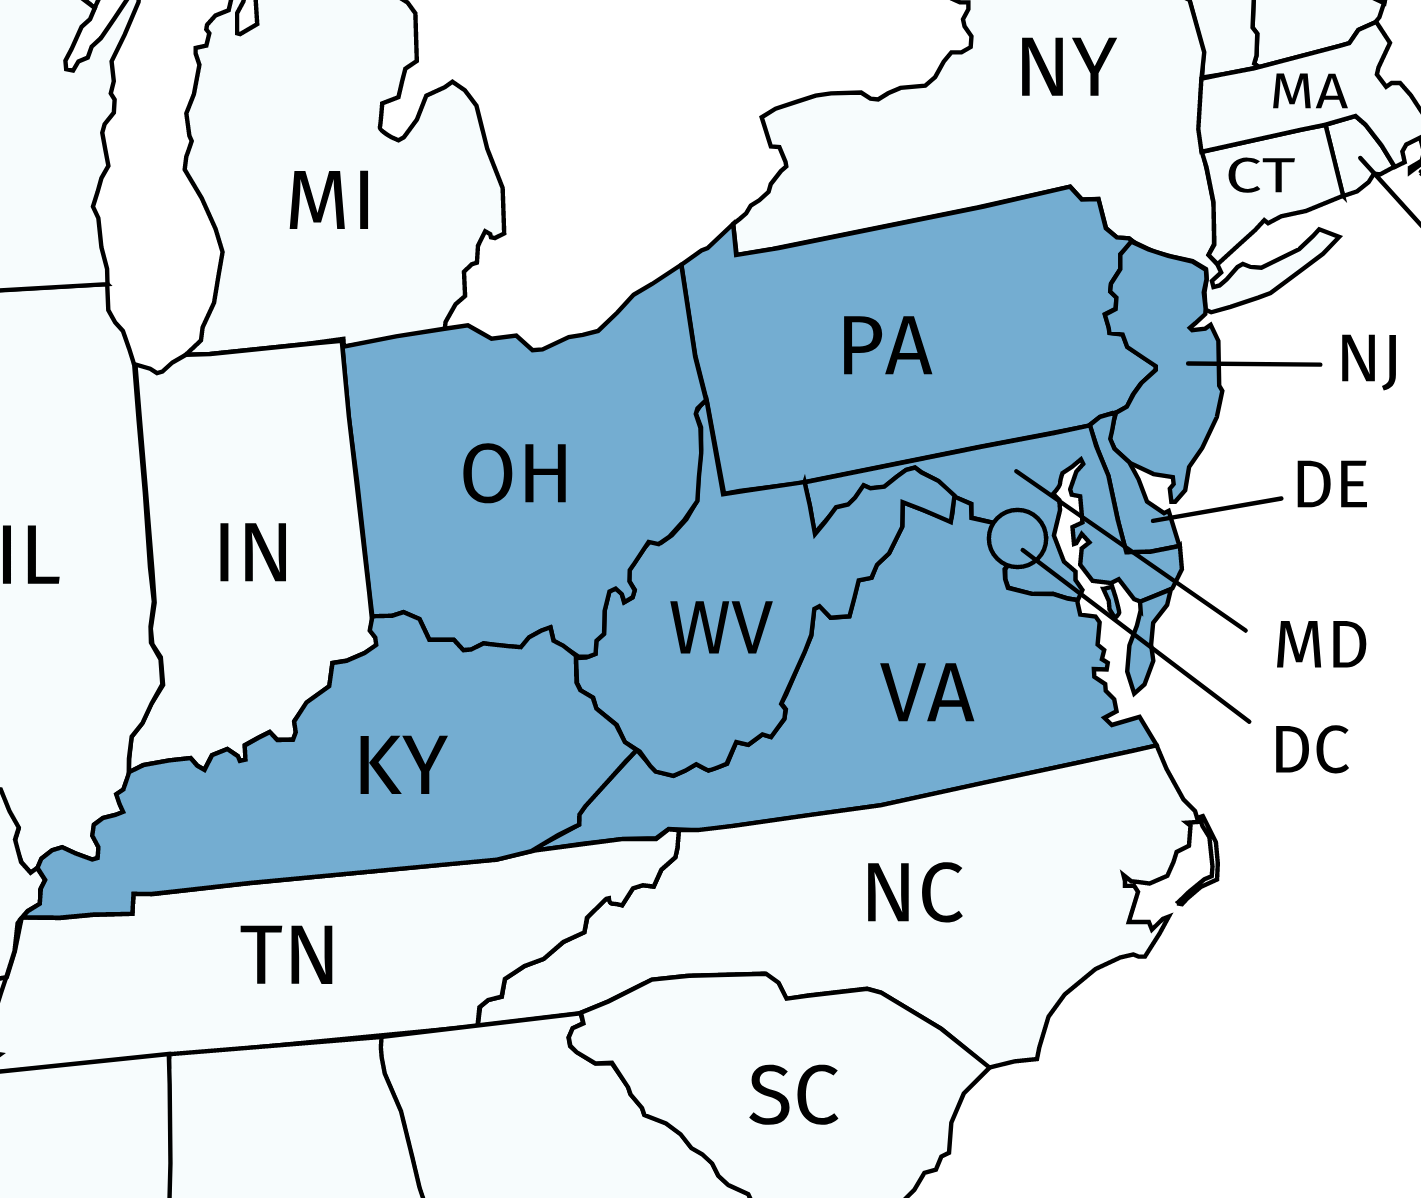
\includegraphics[height=1.5in]{selected_states_around_md_cropped}
&
\begin{tikzpicture}
  \GraphInit[vstyle=simple]
  \tikzset{VertexStyle/.append style={scale=0.3}}
  \SetGraphUnit{1.8}
  
  \grEmptyCycle[RA=2,prefix=a]{8}
  \grEmptyCycle[RA=0,prefix=b]{1}
  
  \extralabel[1mm]{a0}{0}{MD}
  \extralabel[1mm]{a1}{45}{DE}
  \extralabel[1mm]{a2}{90}{NJ}
  \extralabel[1mm]{a3}{135}{PA}
  \extralabel[1mm]{a4}{180}{OH}
  \extralabel[1mm]{a5}{225}{KY}
  \extralabel[1mm]{a6}{-90}{VA}
  \extralabel[1mm]{a7}{-45}{DC}
  \extralabel[1mm]{b0}{-45}{WV}
  
  %\tikzset{EdgeStyle/.style = {->-,>=latex[round]}}
  \Edge(a0)(a1)
  \Edge(a0)(a3)
  \Edge(a0)(a6)
  \Edge(a0)(a7)
  \Edge(a0)(b0)
  \Edge(a1)(a2)
  \Edge(a1)(a3)
  \Edge(a2)(a3)
  \Edge(a3)(a4)
  \Edge(a3)(b0)
  \Edge(a4)(a5)
  \Edge(a4)(b0)
  \Edge(a5)(a6)
  \Edge(a5)(b0)
  \Edge(a6)(a7)
  \Edge(a6)(b0)
\end{tikzpicture}
\end{tabular}
\end{center}
\pagebreak

\item The map below shows eight countries in Asia highlighted in blue.  Draw a graph to represent this map, where each node represents a country, and an edge represents a shared border between two countries.
\begin{center}
\begin{tabular}{c c}
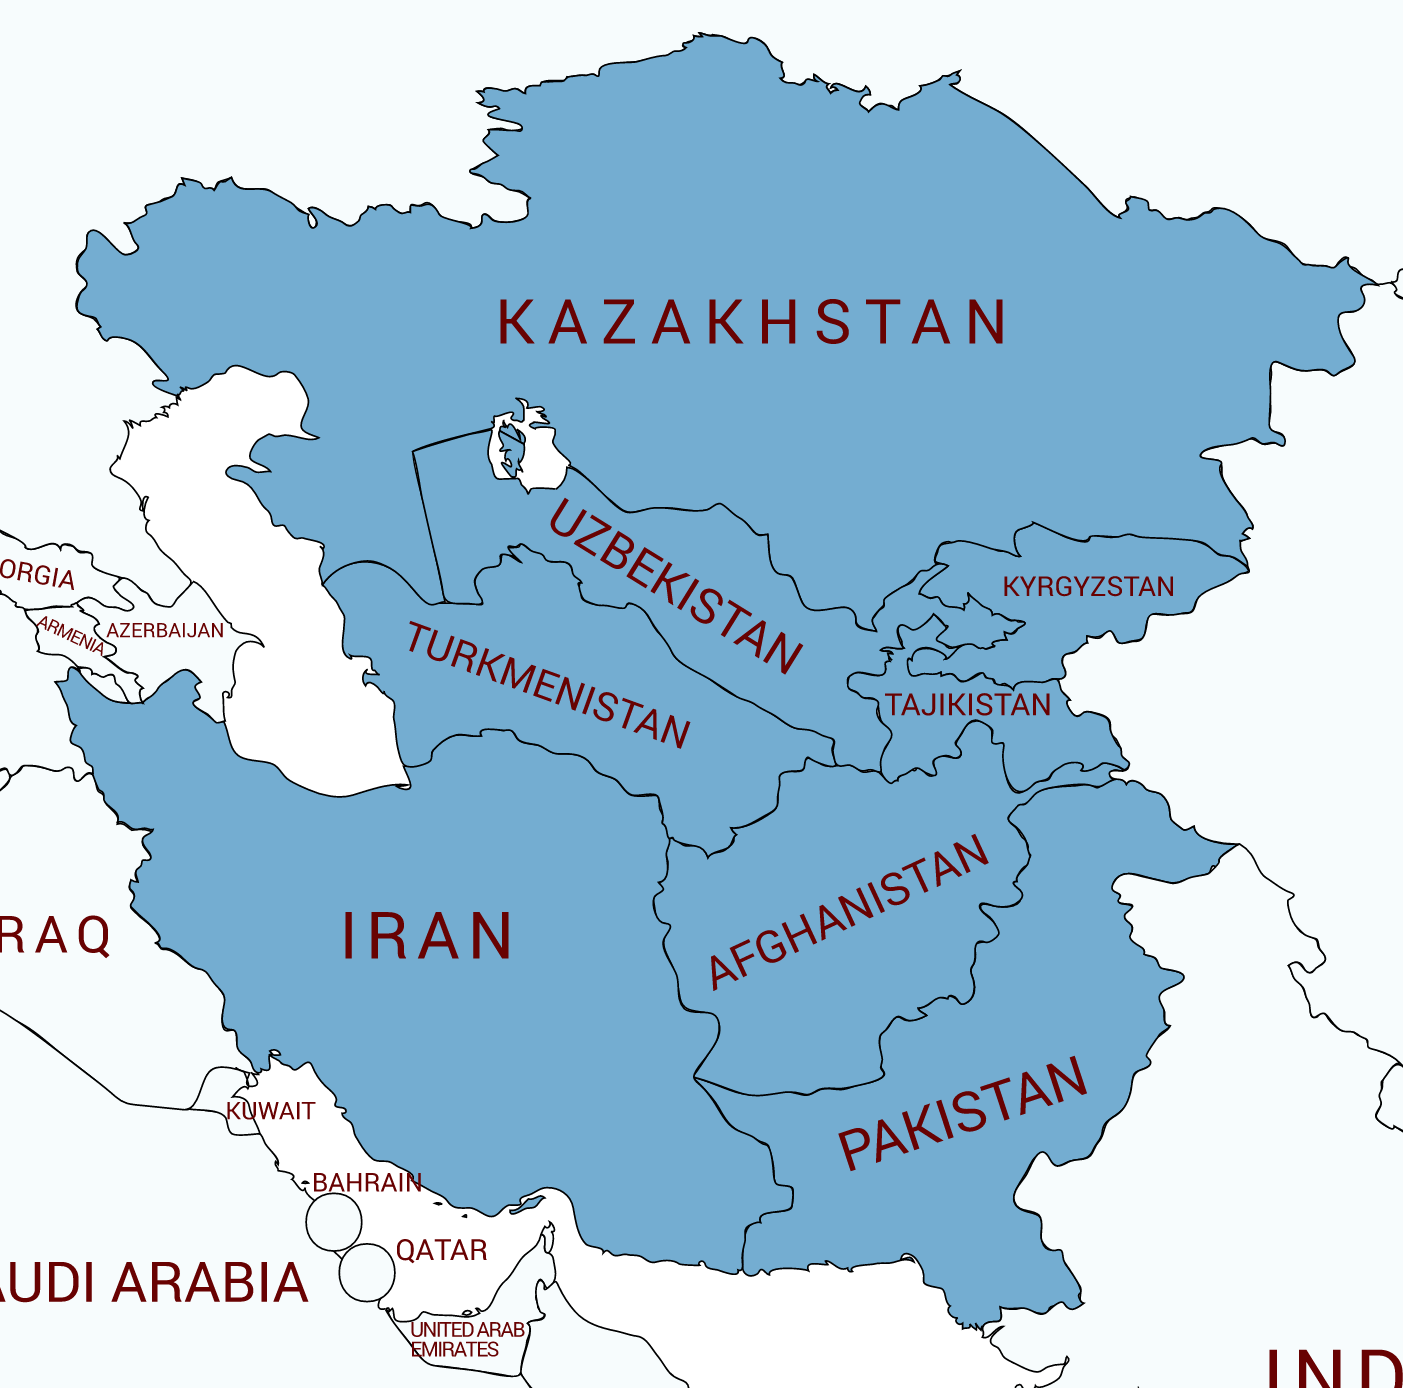
\includegraphics[height=2in]{middle_east_countries_cropped}
&
\begin{tikzpicture}
  \GraphInit[vstyle=simple]
  \tikzset{VertexStyle/.append style={scale=0.3}}
  \SetGraphUnit{1.8}
  
  \grEmptyCycle[RA=2,prefix=a]{7}
  \grEmptyCycle[RA=0,prefix=b]{1}
  
  \extralabel[1mm]{a0}{0}{Taj.}
  \extralabel[1mm]{a1}{45}{Kyr.}
  \extralabel[1mm]{a2}{90}{Kaz.}
  \extralabel[1mm]{a3}{135}{Uzb.}
  \extralabel[1mm]{a4}{180}{Tur.}
  \extralabel[1mm]{a5}{225}{Iran}
  \extralabel[1mm]{a6}{-90}{Pak.}
  \extralabel[1mm]{b0}{-45}{Afg.}
  
  %\tikzset{EdgeStyle/.style = {->-,>=latex[round]}}
  \Edge(a0)(a1)
  \Edge(a0)(a3)
  \Edge(a0)(b0)
  \Edge(a1)(a2)
  \Edge(a1)(a3)
  \Edge(a2)(a3)
  \Edge(a2)(a4)
  \Edge(a3)(a4)
  \Edge(a3)(b0)
  \Edge(a4)(a5)
  \Edge(a4)(b0)
  \Edge(a5)(a6)
  \Edge(a5)(b0)
  \Edge(a6)(b0)
\end{tikzpicture}
\end{tabular}
\end{center}

\item The graph below represents a tournament; each edge marks a game between two teams.
\begin{center}
\begin{tikzpicture}
  \GraphInit[vstyle=simple]
  \tikzset{VertexStyle/.append style={scale=0.3}}
  \SetGraphUnit{1}
  
  \grEmptyCycle[RA=1.5,rotation=18,prefix=a]{5}
  
  \extralabel[1mm]{a0}{0}{Warriors}
  \extralabel[1mm]{a1}{90}{Hawks}
  \extralabel[1mm]{a2}{180}{Hornets}
  \extralabel[1mm]{a3}{-90}{Lions}
  \extralabel[1mm]{a4}{-90}{Bears}
  
  \Edge(a1)(a0)
  \Edge(a1)(a3)
  \Edge(a2)(a4)
  \Edge(a2)(a0)
  \Edge(a4)(a0)
  \Edge(a2)(a3)
  \Edge(a0)(a3)
\end{tikzpicture}
\end{center}
\begin{enumerate}[(a)]
\item Did the Hornets and the Hawks play each other? \answersub{No}
\item How many games do the Warriors play? \answersub{4}
\item Which teams do the Bears play? \answersub{Hornets and Warriors}
\item Which team(s) played the most games? \answersub{Warriors}
\item Which team(s) played the fewest games? \answersub{Hawks and Bears (each played 2)}
\end{enumerate}

\item The graph below is an \emph{influence graph}, where each edge represents the influence that one person has on another; the arrow goes from the influencer to the one they influence.
\begin{center}
\begin{tikzpicture}
  \GraphInit[vstyle=simple]
  \tikzset{VertexStyle/.append style={scale=0.3}}
  \SetGraphUnit{1.8}
  
  \Vertex{Joelle}
  \EA(Joelle){Jonathan}
  \SO(Joelle){Anastasia}
  \SO(Jonathan){Laila}
  \EA(Laila){Zachary}
  
  \extralabel[1mm]{Joelle}{90}{Joelle}
  \extralabel[1mm]{Jonathan}{90}{Jonathan}
  \extralabel[1mm]{Anastasia}{-90}{Anastasia}
  \extralabel[1mm]{Laila}{-90}{Laila}
  \extralabel[1mm]{Zachary}{0}{Zachary}
  
  \tikzset{EdgeStyle/.style = {->-,>=latex[round]}}
  \Edge(Zachary)(Jonathan)
  \Edge(Zachary)(Laila)
  \Edge(Zachary)(Joelle)
  \Edge(Anastasia)(Jonathan)
  \Edge(Joelle)(Laila)
  \Edge(Laila)(Jonathan)
  \Edge(Anastasia)(Joelle)
\end{tikzpicture}
\end{center}
\begin{enumerate}[(a)]
\item Who does Laila influence? \answersub{Jonathan}
\item Does Jonathan influence Anastasia? \answersub{No}
\item How many people does Joelle influence? \answersub{1}
\item Who is the most influential (influences the most people)? \answersub{Zachary (3)}
\item Who is the most influenced (influenced by the most people)? \answersub{Jonathan (3)}
\end{enumerate}
\end{enumerate}

\emph{For problems 7--10, describe a graph that could be used to model the given application.  Specifically, answer the following questions:
\begin{enumerate}[(a)]
\item Are loops allowed in this graph?
\item Are multiple edges allowed between the same pair of nodes?
\item Is this a simple graph or multigraph?
\item Is this graph directed or undirected?
\item Is this a complete graph (generally)?
\end{enumerate}}

\begin{enumerate}
\setcounter{enumi}{6}

\item Flights between major cities, if each node represents a city and each edge describes a flight from one city to another (or from a city to itself, if there is a sightseeing or training flight).
\begin{enumerate}[(a)]
\item Are loops allowed in this graph? \answersub{Yes}
\item Are multiple edges allowed between the same pair of nodes? \answersub{Yes}
\item Is this a simple graph or multigraph? \answersub{Multigraph}
\item Is this graph directed or undirected? \answersub{Directed}
\item Is this a complete graph (generally)? \answersub{No}
\end{enumerate}

\item A party, where each node represents a person, and each edge represents whether one person knows the name of another.
\begin{enumerate}[(a)]
\item Are loops allowed in this graph? \answersub{Yes}
\item Are multiple edges allowed between the same pair of nodes? \answersub{Yes}
\item Is this a simple graph or multigraph? \answersub{Multigraph}
\item Is this graph directed or undirected? \answersub{Directed}
\item Is this a complete graph (generally)? \answersub{No}
\end{enumerate}

\item The floorplan of a house, where each node represents a room or space (like a hallway), and each edge represents a doorway.
\begin{enumerate}[(a)]
\item Are loops allowed in this graph? \answersub{No}
\item Are multiple edges allowed between the same pair of nodes? \answersub{Yes}
\item Is this a simple graph or multigraph? \answersub{Multigraph}
\item Is this graph directed or undirected? \answersub{Undirected}
\item Is this a complete graph (generally)? \answersub{No}
\end{enumerate}

\item Courses offered at a college, where each node represents a course, and each edge represents a prerequisite requirement.
\begin{enumerate}[(a)]
\item Are loops allowed in this graph? \answersub{No}
\item Are multiple edges allowed between the same pair of nodes? \answersub{No}
\item Is this a simple graph or multigraph? \answersub{Simple}
\item Is this graph directed or undirected? \answersub{Directed}
\item Is this a complete graph (generally)? \answersub{No}
\end{enumerate}
\end{enumerate}

\emph{For problems 11--14, answer the following questions for the given graph:
\begin{enumerate}[(a)]
\item Is it a simple graph or multigraph?
\item Is it directed or undirected?
\end{enumerate}}

\begin{enumerate}
\setcounter{enumi}{10}

\item \text{} \answer{(a) Multigraph (b) Undirected} 
\begin{center}
\begin{tikzpicture}
  \GraphInit[vstyle=simple]
  \tikzset{VertexStyle/.append style={scale=0.3}}
  \SetGraphUnit{2.2}
  
  \Vertex{a}
  \EA(a){b}
  \SO(a){c}
  \SO(b){d}
  
  \extralabel[1mm]{a}{90}{$a$}
  \extralabel[1mm]{b}{90}{$b$}
  \extralabel[1mm]{c}{-90}{$c$}
  \extralabel[1mm]{d}{-90}{$d$}
  
  %\tikzset{EdgeStyle/.style = {->-,>=latex[round]}}
  %\SetUpEdge[style={bend right=30}]
  %\Loop[dist=1.5cm,dir=NO,style={-}](NYC)
  \Edge(a)(b)
  \Edge(b)(d)
  \Edge(b)(c)
  \SetUpEdge[style={bend right=30}]
  \Edge(a)(d)
  \Edge(d)(a)
\end{tikzpicture}
\end{center}

\item \text{} \answer{(a) Multigraph (b) Directed} 
\begin{center}
\begin{tikzpicture}
  \GraphInit[vstyle=simple]
  \tikzset{VertexStyle/.append style={scale=0.3}}
  \SetGraphUnit{2.2}
  
  \Vertex{a}
  \EA(a){b}
  \SO(a){c}
  \SO(b){d}
  
  \extralabel[1mm]{a}{90}{$a$}
  \extralabel[1mm]{b}{90}{$b$}
  \extralabel[1mm]{c}{-90}{$c$}
  \extralabel[1mm]{d}{-90}{$d$}
  
  \tikzset{EdgeStyle/.style = {->-,>=latex[round]}}
  %\SetUpEdge[style={bend right=30}]
  %\Loop[dist=1.5cm,dir=NO,style={-}](NYC)
  \Edge(a)(c)
  \Edge(b)(c)
  \Edge(d)(b)
  \tikzset{EdgeStyle/.style = {->-,>=latex[round],bend right=30}}
  \Edge(a)(b)
  \Edge(b)(a)
\end{tikzpicture}
\end{center}

\item \text{} \answer{(a) Multigraph (b) Undirected} 
\begin{center}
\begin{tikzpicture}
  \GraphInit[vstyle=simple]
  \tikzset{VertexStyle/.append style={scale=0.3}}
  \SetGraphUnit{0.75}
  
  \Vertex{a}
  \EA(a){b}
  \SOEA(b){c}
  \SOWE(c){d}
  \WE(d){e}
  \NOWE(e){f}
  
  \extralabel[1mm]{a}{90}{$a$}
  \extralabel[1mm]{b}{0}{$b$}
  \extralabel[1mm]{c}{0}{$c$}
  \extralabel[1mm]{d}{-90}{$d$}
  \extralabel[1mm]{e}{-90}{$e$}
  \extralabel[1mm]{f}{180}{$f$}
  
  %\tikzset{EdgeStyle/.style = {->-,>=latex[round]}}
  %\SetUpEdge[style={bend right=30}]
  \Loop[dist=1.2cm,dir=NO,style={-}](b)
  \Loop[dist=1.2cm,dir=WE,style={-}](e)
  \Edge(a)(b)
  \Edge(a)(b)
  \Edge(b)(c)
  \SetUpEdge[style={bend right=15}]
  \Edge(a)(d)
  \Edge(d)(a)
  \Edge(a)(e)
  \Edge(e)(f)
  \Edge(a)(d)
  \Edge(c)(f)
\end{tikzpicture}
\end{center}

\item \text{} \answer{(a) Simple graph (b) Directed} 
\begin{center}
\begin{tikzpicture}
  \GraphInit[vstyle=simple]
  \tikzset{VertexStyle/.append style={scale=0.3}}
  \SetGraphUnit{1.8}
  
  \Vertex{a}
  \EA(a){b}
  \SO(a){c}
  \SO(b){d}
  \EA(b){e}
  
  \extralabel[1mm]{a}{90}{$a$}
  \extralabel[1mm]{b}{90}{$b$}
  \extralabel[1mm]{c}{-90}{$c$}
  \extralabel[1mm]{d}{-90}{$d$}
  \extralabel[1mm]{e}{0}{$e$}
  
  \tikzset{EdgeStyle/.style = {->-,>=latex[round]}}
  \Edge(a)(b)
  \Edge(c)(a)
  \Edge(a)(d)
  \Edge(b)(e)
  \Edge(e)(d)
  \Edge(d)(b)
\end{tikzpicture}
\end{center}
\end{enumerate}

\emph{For problems 15--17, determine the degree of each node.  For the directed graphs, determine both the in-degree and the out-degree of each node.}

\begin{enumerate}
\setcounter{enumi}{14}

\item \text{} \begin{center}
\begin{tikzpicture}
  \GraphInit[vstyle=simple]
  \tikzset{VertexStyle/.append style={scale=0.3}}
  \SetGraphUnit{2}
  
  \Vertex{a}
  \EA(a){b}
  \SO(a){c}
  \SO(b){d}
  \EA(b){e}
  
  \extralabel[1mm]{a}{90}{$a$}
  \extralabel[1mm]{b}{90}{$b$}
  \extralabel[1mm]{c}{-90}{$c$}
  \extralabel[1mm]{d}{-90}{$d$}
  \extralabel[1mm]{e}{0}{$e$}
  
  \tikzset{EdgeStyle/.style = {->-,>=latex[round]}}
  \Loop[dist=1.2cm,dir=NO,style={->-}](b)
  \Edge(b)(c)
  \Edge(d)(e)
  \Edge(d)(b)
  \tikzset{EdgeStyle/.style = {->-,>=latex[round],bend right=15}}
  \Edge(a)(c)
  \Edge(c)(a)
  \Edge(b)(e)
  \Edge(e)(b)
\end{tikzpicture}
\end{center}
\begin{center}
\begin{tabular}{c c c}
\textbf{Node} & \textbf{In-Degree} & \textbf{Out-Degree}\\
\hline
$a$ & 1 & 1\\
$b$ & 3 & 3\\
$c$ & 2 & 1\\
$d$ & 0 & 2\\
$e$ & 2 & 1
\end{tabular}
\end{center}

\item \text{} \begin{center}
\begin{tikzpicture}
  \GraphInit[vstyle=simple]
  \tikzset{VertexStyle/.append style={scale=0.3}}
  
  \grEmptyCycle[RA=1.7,prefix=a]{6}
  
  \extralabel[1mm]{a0}{0}{$a$}
  \extralabel[1mm]{a1}{90}{$b$}
  \extralabel[1mm]{a2}{90}{$c$}
  \extralabel[1mm]{a3}{180}{$d$}
  \extralabel[1mm]{a4}{-90}{$e$}
  \extralabel[1mm]{a5}{-90}{$f$}
  
  %\tikzset{EdgeStyle/.style = {->-,>=latex[round]}}
  %\SetUpEdge[style={bend right=30}]
  %\Loop[dist=1.5cm,dir=NO,style={-}](NYC)
  \Edge(a0)(a1)
  \Edge(a0)(a3)
  \Edge(a1)(a4)
  \Edge(a2)(a4)
  \Edge(a3)(a5)
  \SetUpEdge[style={bend right=20}]
  \Edge(a1)(a5)
  \Edge(a5)(a1)
\end{tikzpicture}
\end{center}
\begin{center}
\begin{tabular}{c c}
\textbf{Node} & \textbf{Degree}\\
\hline
$a$ & 2\\
$b$ & 4\\
$c$ & 1\\
$d$ & 2\\
$e$ & 2\\
$f$ & 3
\end{tabular}
\end{center}
\pagebreak

\item \text{} \begin{center}
\begin{tikzpicture}
  \GraphInit[vstyle=simple]
  \tikzset{VertexStyle/.append style={scale=0.3}}
  \grComplete[RA=1.7,prefix=a]{7}
  
  \extralabel[1mm]{a0}{0}{$a$}
  \extralabel[1mm]{a1}{45}{$b$}
  \extralabel[1mm]{a2}{90}{$c$}
  \extralabel[1mm]{a3}{135}{$d$}
  \extralabel[1mm]{a4}{180}{$e$}
  \extralabel[1mm]{a5}{-90}{$f$}
  \extralabel[1mm]{a6}{-45}{$g$}
\end{tikzpicture}
\end{center}
\begin{center}
\begin{tabular}{c c}
\textbf{Node} & \textbf{Degree}\\
\hline
$a$ & 6\\
$b$ & 6\\
$c$ & 6\\
$d$ & 6\\
$e$ & 6\\
$f$ & 6\\
$g$ & 6
\end{tabular}
\end{center}
\end{enumerate}

\section{Euler and Hamilton Paths}
\emph{In problems 1--3, determine whether the given graph is connected or disconnected.}

\begin{enumerate}
\item \begin{center}
\begin{tikzpicture}
  \GraphInit[vstyle=simple]
  \tikzset{VertexStyle/.append style={scale=0.3}}
  \SetGraphUnit{2}
  
  \Vertex{a}
  \EA(a){b}
  \EA(b){c}
  \SO(a){d}
  \SO(b){e}
  
  \Edge(a)(d)
  \Edge(a)(e)
  \Edge(b)(c)
  \Edge(b)(d)
  \Edge(b)(e)
  \Edge(c)(e)
\end{tikzpicture}
\end{center}

\item \begin{center}
\begin{tikzpicture}
  \GraphInit[vstyle=simple]
  \tikzset{VertexStyle/.append style={scale=0.3}}
  \SetGraphUnit{1}
  
  \Vertex{a}
  \NOEA(a){b}
  \EA(b){c}
  \EA(c){d}
  \EA(d){e}
  \EA(e){f}
  \EA(a){g}
  \EA(g){h}
  \EA(h){i}
  \EA(i){j}
  \EA(j){k}
  
  \Edge(a)(b)
  \Edge(b)(h)
  \Edge(h)(d)
  \Edge(d)(j)
  \Edge(j)(f)
  \Edge(g)(c)
  \Edge(c)(i)
  \Edge(i)(e)
  \Edge(e)(k)
\end{tikzpicture}
\end{center}

\item \begin{center}
\begin{tikzpicture}
  \GraphInit[vstyle=simple]
  \tikzset{VertexStyle/.append style={scale=0.3}}
  \SetGraphUnit{2}
  
  \grEmptyCycle[RA=1.5,rotation=30,prefix=a]{6}
  
  \Edge(a0)(a2)
  \Edge(a2)(a4)
  \Edge(a4)(a0)
  \Edge(a1)(a3)
  \Edge(a3)(a5)
  \Edge(a5)(a1)
\end{tikzpicture}
\end{center}
\end{enumerate}

\emph{In problems 4--16, determine whether the given graph has an Euler circuit (and draw one if it exists).  If not, determine whether it has an Euler path (and draw one if so).}
\begin{enumerate}
\setcounter{enumi}{3}

\item \begin{center} %4
\begin{tikzpicture}
  \GraphInit[vstyle=simple]
  \tikzset{VertexStyle/.append style={scale=0.3}}
  \SetGraphUnit{1.3}
  \Vertex{a}
  \SOEA(a){e}
  \NOEA(e){b}
  \SOWE(e){c}
  \SOEA(e){d}
  
  \extralabel{a}{90}{$a$}
  \extralabel{b}{90}{$b$}
  \extralabel{c}{-90}{$c$}
  \extralabel{d}{-90}{$d$}
  \extralabel{e}{-90}{$e$}
  
  \Edge(a)(b)
  \Edge(a)(e)
  \Edge(a)(c)
  \Edge(b)(d)
  \Edge(d)(c)
  \Edge(d)(e)
  \SetUpEdge[style={bend right=20}]
  \Edge(b)(e)
  \Edge(e)(b)
  \Edge(c)(e)
  \Edge(e)(c)
\end{tikzpicture}
\end{center}

\item \begin{center} %5
\begin{tikzpicture}
  \GraphInit[vstyle=simple]
  \tikzset{VertexStyle/.append style={scale=0.3}}
  \SetGraphUnit{0.9}
  \Vertex{a}
  \SOEA(a){b}
  \SOWE(b){d}
  \SOWE(a){f}
  \SOEA(d){c}
  \SOWE(d){e}
  
  \extralabel{a}{90}{$a$}
  \extralabel{b}{0}{$b$}
  \extralabel{c}{-90}{$c$}
  \extralabel{d}{135}{$d$}
  \extralabel{e}{-90}{$e$}
  \extralabel{f}{180}{$f$}
  
  \Edge(a)(b)
  \Edge(a)(d)
  \Edge(a)(f)
  \Edge(b)(c)
  \Edge(b)(d)
  \Edge(b)(f)
  \Edge(c)(d)
  \Edge(c)(e)
  \Edge(d)(e)
  \Edge(e)(f)
  \SetUpEdge[style={bend right=15}]
  \Edge(a)(e)
\end{tikzpicture}
\end{center}

\item \begin{center} %6
\begin{tikzpicture}
  \GraphInit[vstyle=simple]
  \tikzset{VertexStyle/.append style={scale=0.3}}
  \SetGraphUnit{1.5}
  \Vertex{a}
  \EA(a){b}
  \EA(b){c}
  \SO(a){e}
  \SO(b){d}
  
  \extralabel{a}{90}{$a$}
  \extralabel{b}{90}{$b$}
  \extralabel{c}{0}{$c$}
  \extralabel{d}{-90}{$d$}
  \extralabel{e}{225}{$e$}
  
  \Edge(a)(b)
  \Edge(a)(e)
  \Edge(b)(c)
  \Edge(b)(d)
  \Edge(b)(e)
  \Edge(d)(e)
  \Edge(c)(e)
  \SetUpEdge[style={bend right=20}]
  \Edge(c)(d)
  \Edge(d)(c)
  \Edge(a)(e)
  \Edge(e)(a)
\end{tikzpicture}
\end{center}

\item \begin{center} %7
\begin{tikzpicture}
  \GraphInit[vstyle=simple]
  \tikzset{VertexStyle/.append style={scale=0.3}}
  \SetGraphUnit{0.75}
  \Vertex{a}
  \NOEA(a){b}
  \SOEA(a){h}
  \SOEA(b){i}
  \NOEA(i){c}
  \SOEA(i){g}
  \SOEA(c){d}
  \EA(d){e}
  \SOEA(d){f}
  
  \extralabel{a}{180}{$a$}
  \extralabel{b}{90}{$b$}
  \extralabel{c}{90}{$c$}
  \extralabel{d}{45}{$d$}
  \extralabel{e}{0}{$e$}
  \extralabel{f}{-90}{$f$}
  \extralabel{g}{-90}{$g$}
  \extralabel{h}{-90}{$h$}
  \extralabel{i}{90}{$i$}
  
  \Edge(a)(b)
  \Edge(a)(h)
  \Edge(a)(i)
  \Edge(b)(c)
  \Edge(b)(i)
  \Edge(c)(d)
  \Edge(c)(i)
  \Edge(d)(e)
  \Edge(d)(f)
  \Edge(d)(g)
  \Edge(d)(i)
  \Edge(e)(f)
  \Edge(g)(i)
  \Edge(h)(i)
  \SetUpEdge[style={bend right=20}]
  \Edge(a)(d)
\end{tikzpicture}
\end{center}

\item \begin{center} %8
\begin{tikzpicture}
  \GraphInit[vstyle=simple]
  \tikzset{VertexStyle/.append style={scale=0.3}}
  \SetGraphUnit{1.3}
  \Vertex{a}
  \SOEA(a){b}
  \SO(b){c}
  \WE(c){d}
  \WE(d){e}
  \NO(e){f}
  
  \extralabel{a}{90}{$a$}
  \extralabel{b}{0}{$b$}
  \extralabel{c}{-90}{$c$}
  \extralabel{d}{-90}{$d$}
  \extralabel{e}{-90}{$e$}
  \extralabel{f}{180}{$f$}
  
  \Edge(a)(b)
  \Edge(a)(f)
  \Edge(b)(d)
  \Edge(b)(f)
  \Edge(c)(d)
  \Edge(d)(e)
  \Edge(e)(f)
\end{tikzpicture}
\end{center}

\item \begin{center} %9
\begin{tikzpicture}
  \GraphInit[vstyle=simple]
  \tikzset{VertexStyle/.append style={scale=0.3}}
  \SetGraphUnit{1.2}
  \Vertex{a}
  \EA(a){b}
  \EA(b){c}
  \EA(c){d}
  \EA(d){e}
  \SO(a){f}
  \EA(f){g}
  \EA(g){h}
  \EA(h){i}
  \EA(i){j}
  \SO(f){k}
  \EA(k){l}
  \EA(l){m}
  \EA(m){n}
  \EA(n){o}
  
  \extralabel{a}{90}{$a$}
  \extralabel{b}{90}{$b$}
  \extralabel{c}{90}{$c$}
  \extralabel{d}{90}{$d$}
  \extralabel{e}{90}{$e$}
  \extralabel{f}{135}{$f$}
  \extralabel{g}{135}{$g$}
  \extralabel{h}{135}{$h$}
  \extralabel{i}{135}{$i$}
  \extralabel{j}{45}{$j$}
  \extralabel{k}{-90}{$k$}
  \extralabel{l}{-90}{$l$}
  \extralabel{m}{-90}{$m$}
  \extralabel{n}{-90}{$n$}
  \extralabel{o}{-90}{$o$}
  
  \Edge(a)(b)
  \Edge(a)(f)
  \Edge(b)(c)
  \Edge(b)(g)
  \Edge(c)(d)
  \Edge(c)(h)
  \Edge(c)(j)
  \Edge(d)(e)
  \Edge(d)(i)
  \Edge(e)(j)
  \Edge(f)(g)
  \Edge(f)(k)
  \Edge(f)(m)
  \Edge(g)(h)
  \Edge(g)(l)
  \Edge(h)(i)
  \Edge(h)(m)
  \Edge(i)(j)
  \Edge(i)(n)
  \Edge(j)(o)
  \Edge(k)(l)
  \Edge(l)(m)
  \Edge(m)(n)
  \Edge(n)(o)
  \SetUpEdge[style={bend right=40}]
  \Edge(d)(b)
  \Edge(l)(n)
\end{tikzpicture}
\end{center}

\item \begin{center} %10
\begin{tikzpicture}
  \GraphInit[vstyle=simple]
  \tikzset{VertexStyle/.append style={scale=0.3}}
  \grCycle[RA=1.5,prefix=a]{8}
  
  \extralabel{a0}{0}{$a$}
  \extralabel{a1}{45}{$b$}
  \extralabel{a2}{90}{$c$}
  \extralabel{a3}{135}{$d$}
  \extralabel{a4}{180}{$e$}
  \extralabel{a5}{225}{$f$}
  \extralabel{a6}{-90}{$g$}
  \extralabel{a7}{-45}{$h$}
  
  \Edge(a0)(a5)
  \Edge(a1)(a6)
  \Edge(a2)(a5)
  \Edge(a2)(a7)
  \Edge(a3)(a6)
  \Edge(a4)(a7)
\end{tikzpicture}
\end{center}

\item \begin{center} %11
\begin{tikzpicture}
  \GraphInit[vstyle=simple]
  \tikzset{VertexStyle/.append style={scale=0.3}}
  \SetGraphUnit{1.3}
  \Vertex{a}
  \EA(a){b}
  \EA(b){c}
  \EA(c){d}
  \SO(d){e}
  \EA(e){f}
  \WE(e){g}
  \WE(g){h}
  \WE(h){i}
  
  \extralabel{a}{90}{$a$}
  \extralabel{b}{90}{$b$}
  \extralabel{c}{90}{$c$}
  \extralabel{d}{90}{$d$}
  \extralabel{e}{-90}{$e$}
  \extralabel{f}{-90}{$f$}
  \extralabel{g}{-90}{$g$}
  \extralabel{h}{-90}{$h$}
  \extralabel{i}{-90}{$i$}
  
  \Edge(a)(b)
  \Edge(a)(h)
  \Edge(a)(i)
  \Edge(b)(c)
  \Edge(b)(h)
  \Edge(b)(i)
  \Edge(c)(d)
  \Edge(c)(e)
  \Edge(c)(g)
  \Edge(c)(i)
  \Edge(d)(e)
  \Edge(d)(g)
  \Edge(d)(h)
  \Edge(e)(f)
  \Edge(g)(h)
  \Edge(h)(i)
  \SetUpEdge[style={bend right=30}]
  \Edge(c)(a)
  \Edge(h)(e)
  \Edge(f)(g)
\end{tikzpicture}
\end{center}

\item \begin{center} %12
\begin{tikzpicture}
  \GraphInit[vstyle=simple]
  \tikzset{VertexStyle/.append style={scale=0.3}}
  \SetGraphUnit{2.6}
  \Vertex{a}
  \EA(a){b}
  \SO(a){c}
  \SO(b){d}
  
  \extralabel{a}{90}{$a$}
  \extralabel{b}{90}{$b$}
  \extralabel{c}{-90}{$c$}
  \extralabel{d}{-90}{$d$}
  
  \tikzset{EdgeStyle/.style = {->-,>=latex[round]}}
  \Edge(a)(b)
  \Edge(a)(d)
  \Edge(c)(a)
  \Edge(c)(b)
  \Edge(d)(c)
  \tikzset{EdgeStyle/.style = {->-,>=latex[round],bend right=20}}
  \Edge(b)(d)
  \Edge(d)(b)
\end{tikzpicture}
\end{center}

\item \begin{center} %13
\begin{tikzpicture}
  \GraphInit[vstyle=simple]
  \tikzset{VertexStyle/.append style={scale=0.3}}
  \SetGraphUnit{2}
  \Vertex{a}
  \EA(a){b}
  \EA(b){c}
  \SO(a){d}
  \EA(d){e}
  
  \extralabel{a}{90}{$a$}
  \extralabel{b}{90}{$b$}
  \extralabel{c}{0}{$c$}
  \extralabel{d}{-90}{$d$}
  \extralabel{e}{-90}{$e$}
  
  \tikzset{EdgeStyle/.style = {->-,>=latex[round]}}
  \Edge(a)(d)
  \Edge(a)(e)
  \Edge(b)(a)
  \Edge(d)(b)
  \tikzset{EdgeStyle/.style = {->-,>=latex[round],bend right=20}}
  \Edge(b)(c)
  \Edge(c)(b)
  \Edge(b)(e)
  \Edge(e)(b)
  \Edge(c)(e)
  \Edge(e)(c)
  \Edge(d)(e)
  \Edge(e)(d)
\end{tikzpicture}
\end{center}

\item \begin{center} %14
\begin{tikzpicture}
  \GraphInit[vstyle=simple]
  \tikzset{VertexStyle/.append style={scale=0.3}}
  \SetGraphUnit{2}
  \Vertex{a}
  \EA(a){b}
  \EA(b){c}
  \SO(a){d}
  \EA(d){e}
  \EA(e){f}
  
  \extralabel{a}{90}{$a$}
  \extralabel{b}{90}{$b$}
  \extralabel{c}{0}{$c$}
  \extralabel{d}{-90}{$d$}
  \extralabel{e}{-90}{$e$}
  \extralabel{f}{-90}{$f$}
  
  \tikzset{EdgeStyle/.style = {->-,>=latex[round]}}
  \Edge(a)(b)
  \Edge(b)(d)
  \Edge(b)(f)
  \Edge(c)(b)
  \Edge(c)(e)
  \Edge(e)(a)
  \Edge(e)(b)
  \Edge(f)(c)
  \Edge(f)(e)
  \tikzset{EdgeStyle/.style = {->-,>=latex[round],bend right=20}}
  \Edge(a)(d)
  \Edge(d)(a)
  \Edge(b)(c)
  \Edge(c)(b)
  \Edge(d)(e)
  \Edge(e)(d)
  \tikzset{EdgeStyle/.style = {->-,>=latex[round],bend right=30}}
  \Edge(d)(f)
\end{tikzpicture}
\end{center}

\item \begin{center} %15
\begin{tikzpicture}
  \GraphInit[vstyle=simple]
  \tikzset{VertexStyle/.append style={scale=0.3}}
  \SetGraphUnit{1.4}
  \Vertex{a}
  \EA(a){b}
  \EA(b){c}
  \EA(c){d}
  \SO(a){e}
  \EA(e){f}
  \EA(f){g}
  \EA(g){h}
  \SO(e){i}
  \EA(i){j}
  \EA(j){k}
  \EA(k){l}
  
  \extralabel{a}{90}{$a$}
  \extralabel{b}{90}{$b$}
  \extralabel{c}{90}{$c$}
  \extralabel{d}{90}{$d$}
  \extralabel{e}{135}{$e$}
  \extralabel{f}{135}{$f$}
  \extralabel{g}{135}{$g$}
  \extralabel{h}{45}{$h$}
  \extralabel{i}{-90}{$i$}
  \extralabel{j}{-90}{$j$}
  \extralabel{k}{-90}{$k$}
  \extralabel{l}{-90}{$l$}
  
  \tikzset{EdgeStyle/.style = {->-,>=latex[round]}}
  \Edge(a)(e)
  \Edge(b)(a)
  \Edge(b)(c)
  \Edge(c)(g)
  \Edge(d)(c)
  \Edge(e)(f)
  \Edge(f)(b)
  \Edge(f)(j)
  \Edge(g)(f)
  \Edge(g)(k)
  \Edge(h)(d)
  \Edge(h)(g)
  \Edge(i)(e)
  \Edge(j)(i)
  \Edge(j)(k)
  \Edge(k)(l)
  \Edge(l)(h)
\end{tikzpicture}
\end{center}

\item \begin{center} %16
\begin{tikzpicture}
  \GraphInit[vstyle=simple]
  \tikzset{VertexStyle/.append style={scale=0.3}}
  \SetGraphUnit{1.4}
  \Vertex{a}
  \SOEA(a){e}
  \NOEA(e){b}
  \SOEA(e){c}
  \SOWE(e){d}
  
  \extralabel{a}{90}{$a$}
  \extralabel{b}{90}{$b$}
  \extralabel{c}{-90}{$c$}
  \extralabel{d}{-90}{$d$}
  \extralabel{e}{135}{$e$}
  
  \tikzset{EdgeStyle/.style = {->-,>=latex[round]}}
  \Edge(a)(b)
  \Edge(b)(e)
  \Edge(c)(b)
  \Edge(d)(c)
  \Edge(d)(a)
  \Edge(e)(d)
\end{tikzpicture}
\end{center}
\end{enumerate}

\emph{In problems 17--19, determine whether the picture shown could be drawn in one continuous motion without lifting the pencil or retracing part of the drawing.}
\begin{enumerate}
\setcounter{enumi}{16}

\item \begin{center} %17
\begin{tikzpicture}
  \GraphInit[vstyle=simple]
  \tikzset{VertexStyle/.append style={scale=0.05}}
  \grCycle[RA=2,rotation=30,prefix=a]{3}
  \grCycle[RA=2,rotation=90,prefix=b]{3}
\end{tikzpicture}
\end{center}

\item \begin{center} %18
\begin{tikzpicture}
  \GraphInit[vstyle=simple]
  \tikzset{VertexStyle/.append style={scale=0.05}}
  \grCycle[RA=0.7]{4}
  \grCycle[RA=1.4]{4}
  \grCycle[RA=2.1]{4}
  \grCycle[RA=2.7]{2}
\end{tikzpicture}
\end{center}

\item \begin{center} %19
\begin{tikzpicture}
  \GraphInit[vstyle=simple]
  \tikzset{VertexStyle/.append style={scale=0.05}}
  \SetGraphUnit{1.2}
  \Vertex{a}
  \SO(a){b}
  \SOWE(b){c}
  \SOEA(b){d}
  \SO(c){e}
  \SO(d){f}
  
  \Edge(a)(b)
  \Edge(b)(c)
  \Edge(b)(d)
  \Edge(c)(d)
  \Edge(d)(f)
  \Edge(e)(f)
  \Edge(c)(e)
  \Edge(c)(f)
  \Edge(d)(e)
\end{tikzpicture}
\end{center}

\item The map below shows ten states highlighted in blue.  Is there a path that a traveler could take through these states in such a way that they cross each border between two states exactly once?
\begin{center}
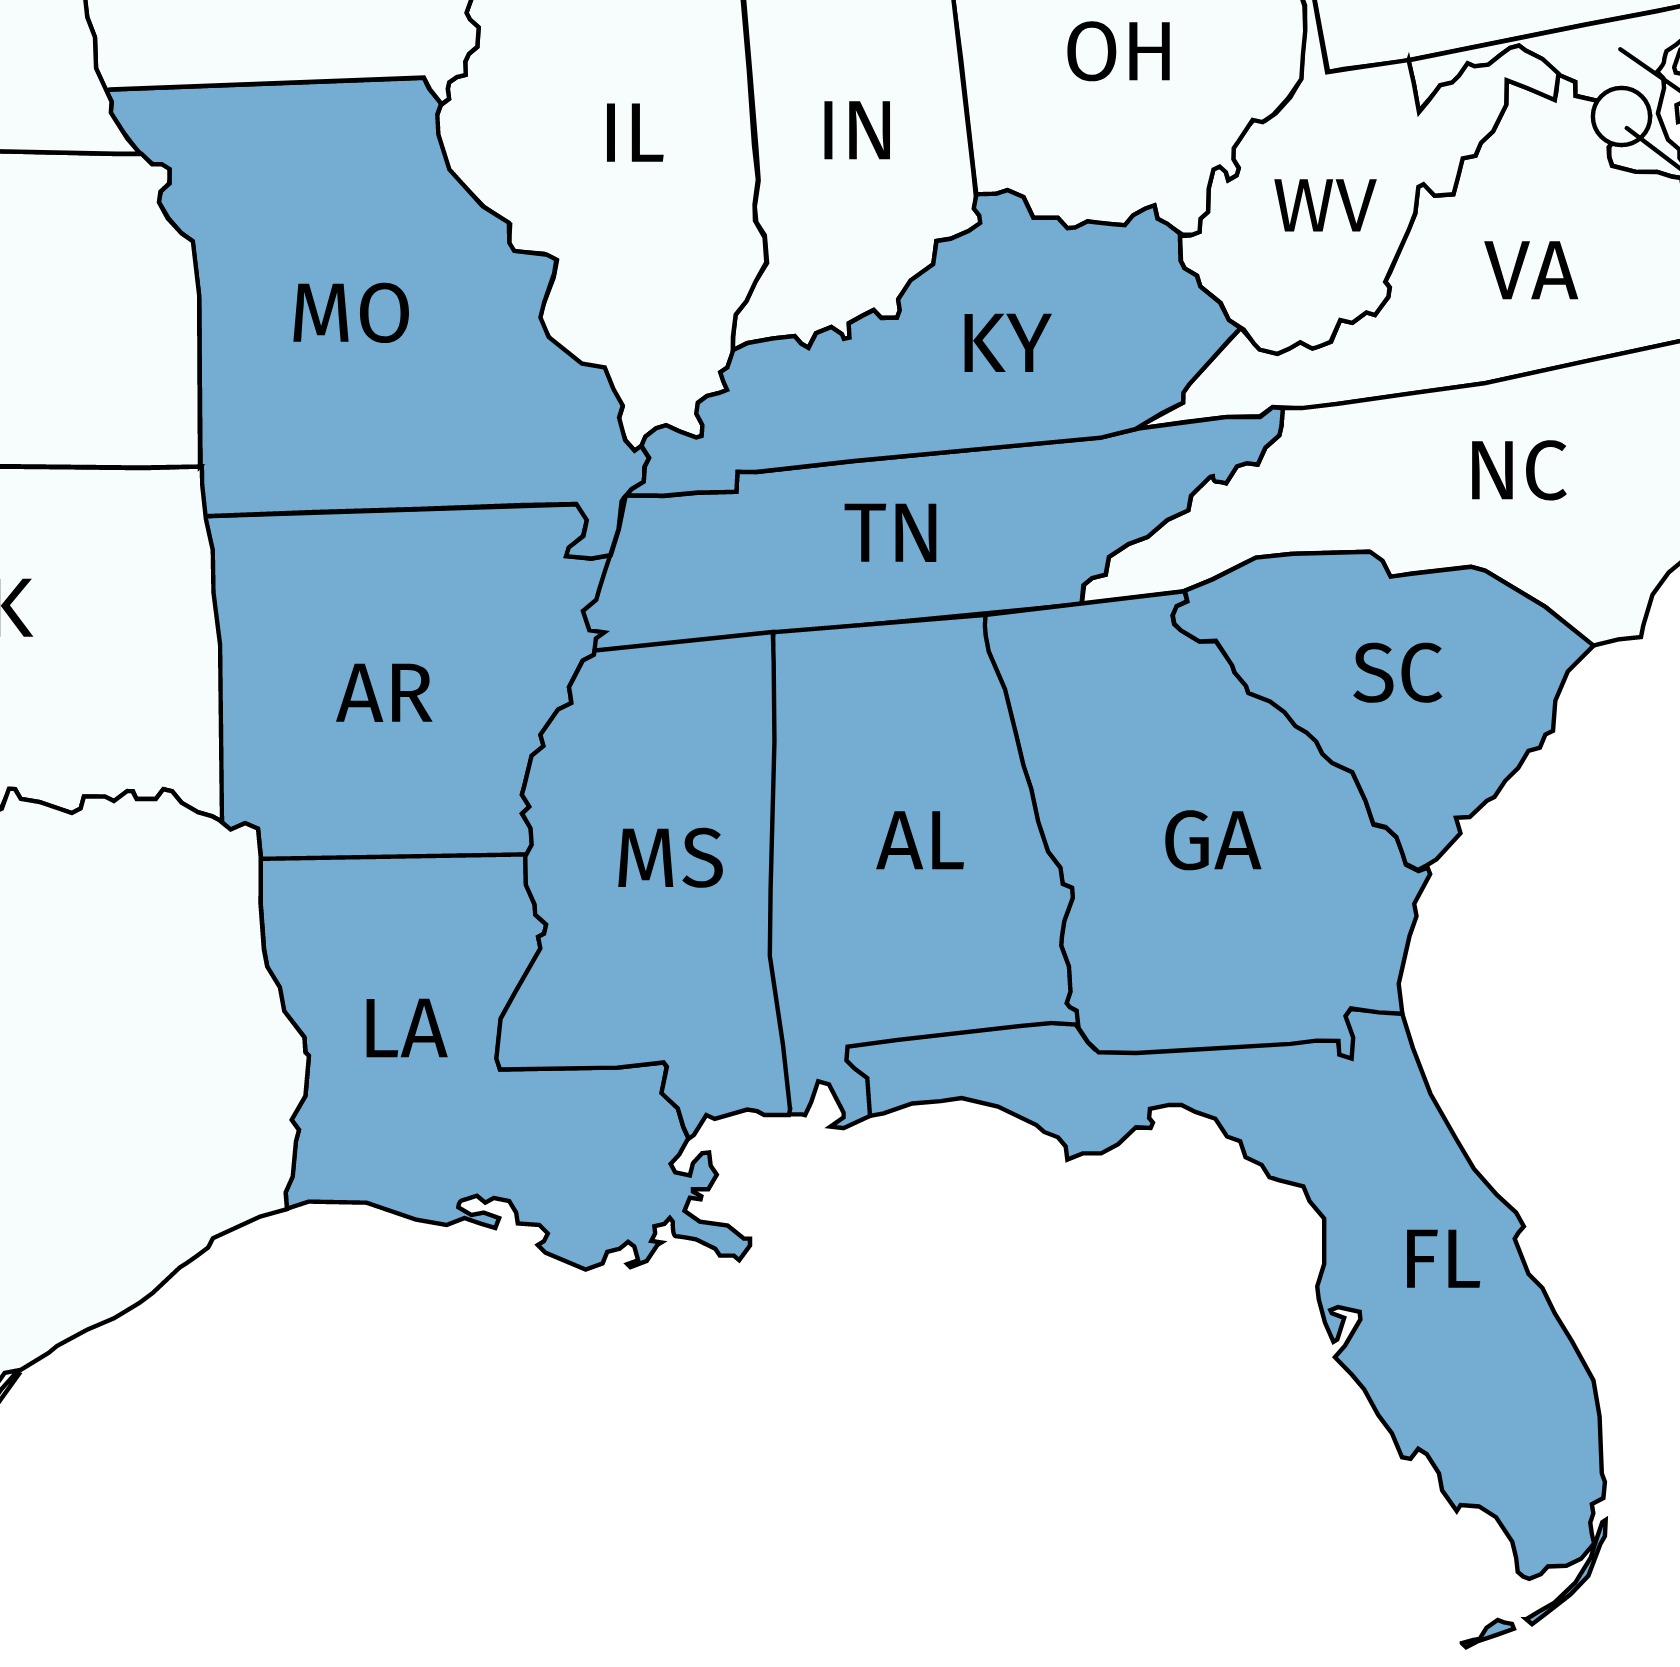
\includegraphics[height=1.7in]{southeast_states2_cropped}
\end{center}

\item France is divided into 18 administrative regions, of which twelve are contiguous.  The map below shows seven of these regions highlighted in blue.  Is there a path that a traveler could take through these regions in such a way that they cross each border between two regions exactly once?
\begin{center}
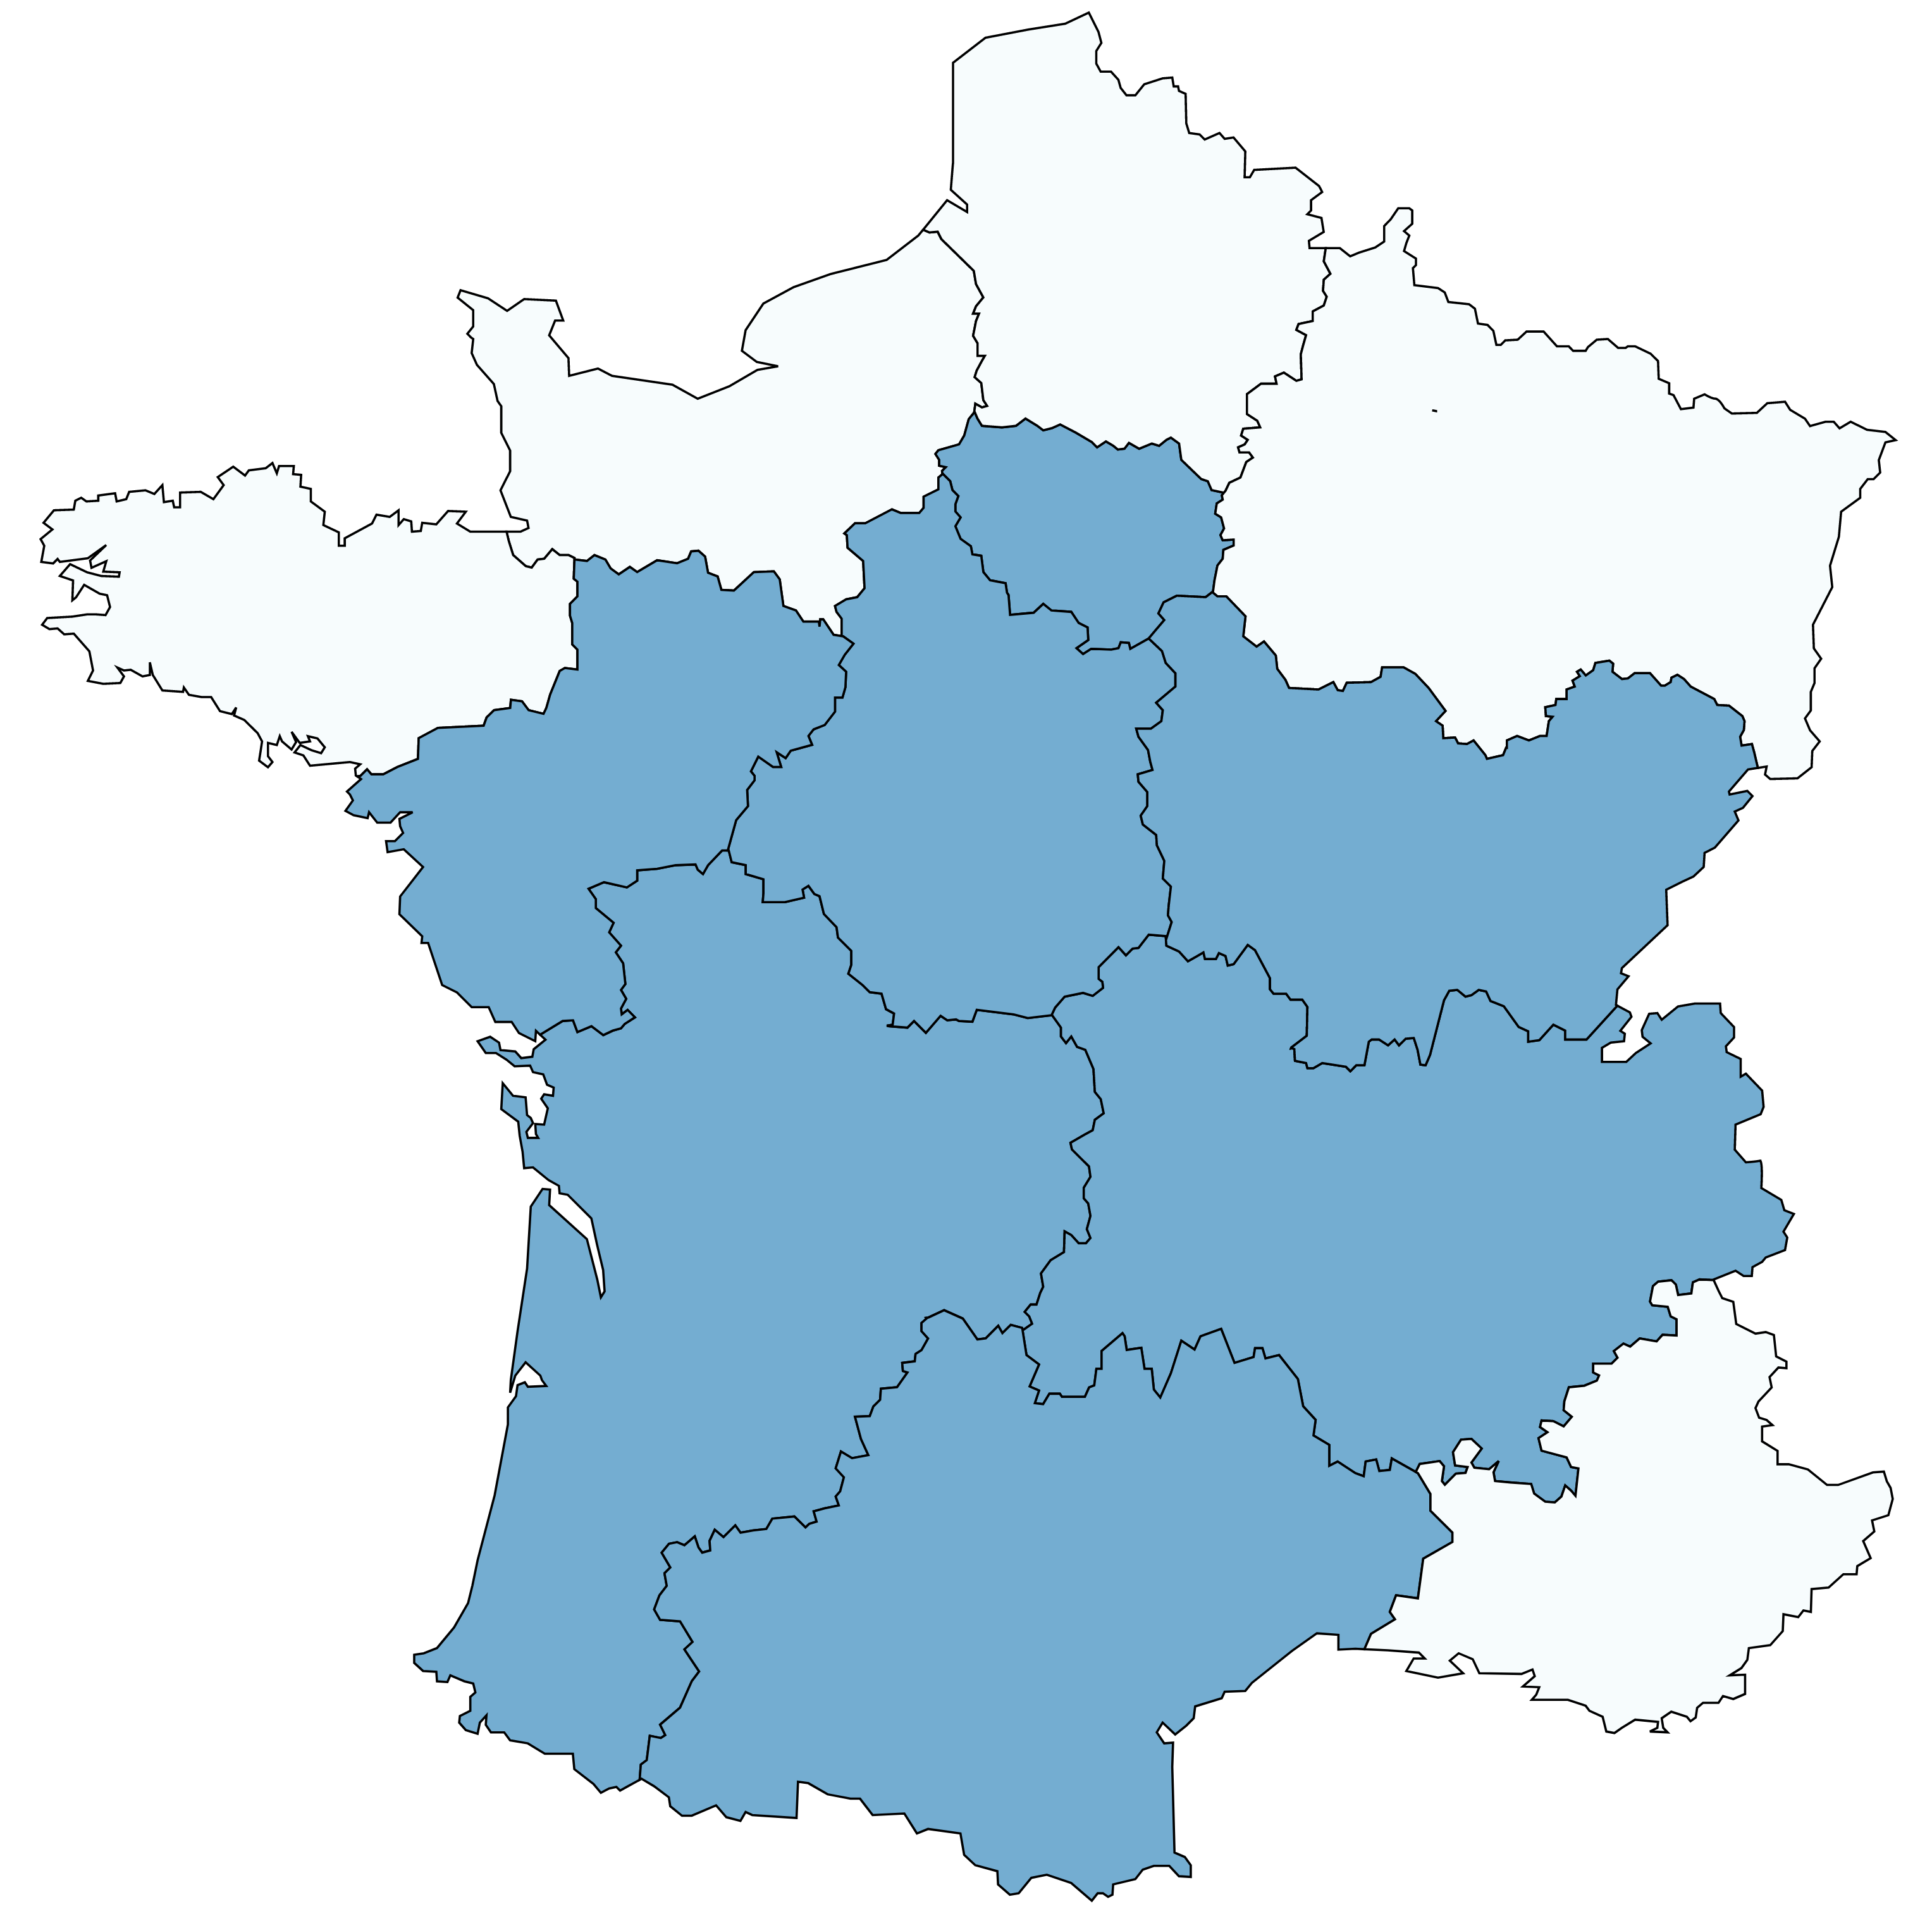
\includegraphics[height=1.6in]{france_states_cropped}
\end{center}
\end{enumerate}

\emph{In problems 22--25, determine whether the given graph has a Hamilton circuit (and draw one if it does).  If not, determine whether it has a Hamilton path (and draw one if so).}
\begin{enumerate}
\setcounter{enumi}{21}

\item \begin{center} %22
\begin{tikzpicture}
  \GraphInit[vstyle=simple]
  \tikzset{VertexStyle/.append style={scale=0.3}}
  \SetGraphUnit{1}
  \Vertex{a}
  \SOEA(a){c}
  \NOEA(c){b}
  \SOWE(c){d}
  \SOEA(c){e}
  \EA(e){f}
  
  \extralabel{a}{90}{$a$}
  \extralabel{b}{90}{$b$}
  \extralabel{c}{225}{$c$}
  \extralabel{d}{-90}{$d$}
  \extralabel{e}{-90}{$e$}
  \extralabel{f}{-90}{$f$}
  
  \Edge(a)(b)
  \Edge(a)(c)
  \Edge(a)(d)
  \Edge(b)(c)
  \Edge(b)(e)
  \Edge(c)(e)
  \Edge(d)(e)
  \Edge(e)(f)
\end{tikzpicture}
\end{center}

\item \begin{center} %23
\begin{tikzpicture}
  \GraphInit[vstyle=simple]
  \tikzset{VertexStyle/.append style={scale=0.3}}
  \SetGraphUnit{1.6}
  \Vertex{a}
  \EA(a){b}
  \EA(b){g}
  \SO(a){c}
  \WE(c){e}
  \EA(c){d}
  \EA(d){f}
  
  \extralabel{a}{90}{$a$}
  \extralabel{b}{90}{$b$}
  \extralabel{c}{-90}{$c$}
  \extralabel{d}{-90}{$d$}
  \extralabel{e}{-90}{$e$}
  \extralabel{f}{-90}{$f$}
  \extralabel{g}{90}{$g$}
  
  \Edge(a)(b)
  \Edge(a)(c)
  \Edge(a)(d)
  \Edge(b)(c)
  \Edge(b)(d)
  \Edge(b)(g)
  \Edge(c)(d)
  \Edge(c)(e)
  \Edge(d)(f)
\end{tikzpicture}
\end{center}

\item \begin{center} %24
\begin{tikzpicture}
  \GraphInit[vstyle=simple]
  \tikzset{VertexStyle/.append style={scale=0.3}}
  \SetGraphUnit{1}
  \Vertex{a}
  \EA(a){b}
  \EA(b){c}
  \SO(a){d}
  \EA(d){e}
  \EA(e){f}
  \SO(d){g}
  \EA(g){h}
  \EA(h){i}
  
  \extralabel{a}{90}{$a$}
  \extralabel{b}{90}{$b$}
  \extralabel{c}{90}{$c$}
  \extralabel{d}{180}{$d$}
  \extralabel[2mm]{e}{15}{$e$}
  \extralabel{f}{0}{$f$}
  \extralabel{g}{-90}{$g$}
  \extralabel{h}{-90}{$h$}
  \extralabel{i}{-90}{$i$}
  
  \Edge(a)(b)
  \Edge(a)(d)
  \Edge(a)(e)
  \Edge(b)(c)
  \Edge(b)(e)
  \Edge(c)(e)
  \Edge(c)(f)
  \Edge(d)(e)
  \Edge(d)(g)
  \Edge(e)(f)
  \Edge(e)(g)
  \Edge(e)(h)
  \Edge(e)(i)
  \Edge(f)(i)
  \Edge(g)(h)
  \Edge(h)(i)
\end{tikzpicture}
\end{center}
\end{enumerate}

\section{Shortest Paths}
\emph{In problems 1-3, use the nearest neighbor algorithm to find a minimum possible circuit through each graph starting at $a$.}
\begin{enumerate}
\item \begin{center}
\begin{tikzpicture}
  \GraphInit[vstyle=simple]
  \tikzset{VertexStyle/.append style={scale=0.3}}
  \grEmptyCycle[prefix=a,RA=1.5]{4}
  
  \extralabel{a0}{0}{$a$}
  \extralabel{a1}{90}{$b$}
  \extralabel{a2}{180}{$c$}
  \extralabel{a3}{-90}{$d$}
  
  \Edge[label=3](a0)(a1)
  \Edge[label=6](a1)(a2)
  \Edge[label=7](a2)(a3)
  \Edge[label=2](a3)(a0)
  \tikzstyle{LabelStyle}=[fill=white,pos=0.3]
  \Edge[label=4](a1)(a3)
  \Edge[label=5](a0)(a2)
\end{tikzpicture}
\end{center}

\item \begin{center}
\begin{tikzpicture}
  \GraphInit[vstyle=simple]
  \tikzset{VertexStyle/.append style={scale=0.3}}
  \grEmptyCycle[prefix=a,RA=1.5,rotation=18]{5}
  
  \extralabel{a0}{0}{$a$}
  \extralabel{a1}{90}{$b$}
  \extralabel{a2}{180}{$c$}
  \extralabel{a3}{-90}{$d$}
  \extralabel{a4}{-90}{$e$}
  
  \Edge[label=3](a0)(a1)
  \Edge[label=10](a1)(a2)
  \Edge[label=6](a2)(a3)
  \Edge[label=1](a3)(a4)
  \Edge[label=7](a4)(a0)
  \Edge[label=8](a0)(a2)
  \Edge[label=4](a0)(a3)
  \Edge[label=9](a1)(a3)
  \Edge[label=2](a1)(a4)
  \Edge[label=5](a2)(a4)
\end{tikzpicture}
\end{center}

\item \begin{center}
\begin{tikzpicture}
  \GraphInit[vstyle=simple]
  \tikzset{VertexStyle/.append style={scale=0.3}}
  \grEmptyCycle[prefix=a,RA=1.5]{6}
  
  \extralabel{a0}{0}{$a$}
  \extralabel{a1}{90}{$b$}
  \extralabel{a2}{90}{$c$}
  \extralabel{a3}{180}{$d$}
  \extralabel{a4}{-90}{$e$}
  \extralabel{a5}{-90}{$f$}
  
  \Edge[label=3](a0)(a1)
  \Edge[label=4](a0)(a5)
  \Edge[label=5](a1)(a2)
  \Edge[label=1](a2)(a3)
  \Edge[label=4](a3)(a4)
  \Edge[label=7](a4)(a5)
  \tikzstyle{LabelStyle}=[fill=white,pos=0.3]
  \Edge[label=2](a0)(a2)
  \Edge[label=3](a0)(a4)
  \Edge[label=6](a3)(a1)
  \Edge[label=3](a3)(a5)
  \tikzstyle{LabelStyle}=[fill=white,pos=0.35]
  \Edge[label=5](a0)(a3)
  \Edge[label=8](a2)(a5)
  \Edge[label=4](a4)(a1)
\end{tikzpicture}
\end{center}
\end{enumerate}

\emph{In problems 4--6, use Dijkstra's algorithm to find the shortest path through each graph between $a$ and $z$.}
\begin{enumerate}
\setcounter{enumi}{3}

\item \begin{center} %4
\begin{tikzpicture}
  \GraphInit[vstyle=simple]
  \tikzset{VertexStyle/.append style={scale=0.3}}
  \SetGraphUnit{0.8}
  
  \Vertex{a}
  \NOEA(a){b}
  \SOEA(a){c}
  \EA(b){d}
  \EA(c){e}
  \NOEA(e){z}
  
  \extralabel{a}{180}{$a$}
  \extralabel{b}{90}{$b$}
  \extralabel{c}{-90}{$c$}
  \extralabel{d}{90}{$d$}
  \extralabel{e}{-90}{$e$}
  \extralabel{z}{0}{$z$}
  
  \Edge[label=2](a)(b)
  \Edge[label=3](a)(c)
  \Edge[label=5](b)(d)
  \Edge[label=2](b)(e)
  \Edge[label=5](c)(e)
  \Edge[label=1](d)(e)
  \Edge[label=2](d)(z)
  \Edge[label=4](e)(z)
\end{tikzpicture}
\end{center}

\item \begin{center} %5
\begin{tikzpicture}
  \GraphInit[vstyle=simple]
  \tikzset{VertexStyle/.append style={scale=0.3}}
  \SetGraphUnit{0.8}
  
  \Vertex{a}
  \NOEA(a){b}
  \SOEA(a){c}
  \EA(b){d}
  \EA(c){e}
  \EA(d){f}
  \EA(e){g}
  \NOEA(g){z}
  
  \extralabel{a}{180}{$a$}
  \extralabel{b}{90}{$b$}
  \extralabel{c}{-90}{$c$}
  \extralabel{d}{90}{$d$}
  \extralabel{e}{-90}{$e$}
  \extralabel{f}{90}{$f$}
  \extralabel{g}{-90}{$g$}
  \extralabel{z}{0}{$z$}
  
  \Edge[label=4](a)(b)
  \Edge[label=3](a)(c)
  \Edge[label=5](b)(d)
  \Edge[label=2](b)(c)
  \Edge[label=3](c)(d)
  \Edge[label=6](c)(e)
  \Edge[label=1](d)(e)
  \Edge[label=5](d)(f)
  \Edge[label=5](e)(g)
  \Edge[label=2](f)(g)
  \Edge[label=7](f)(z)
  \Edge[label=4](g)(z)
\end{tikzpicture}
\end{center}

\item \begin{center} %6
\begin{tikzpicture}
  \GraphInit[vstyle=simple]
  \tikzset{VertexStyle/.append style={scale=0.3}}
  \grEmptyCycle[prefix=a,RA=1.1,rotation=18]{5}
  
  \extralabel{a0}{45}{$a$}
  \extralabel{a1}{90}{$b$}
  \extralabel{a2}{135}{$c$}
  \extralabel{a3}{-90}{$z$}
  \extralabel{a4}{-90}{$e$}
  
  \Edge[label=7](a0)(a1)
  \Edge[label=3](a1)(a2)
  \Edge[label=5](a2)(a3)
  \Edge[label=4](a2)(a4)
  \Edge[label=9](a3)(a4)
  \Edge[label=3](a4)(a0)
  \tikzstyle{LabelStyle}=[fill=white,pos=0.6]
  \Edge[label=6](a0)(a2)
  \Edge[label=7](a1)(a4)
\end{tikzpicture}
\end{center}

\item The graph below shows the distances between cities.  Use the graph to answer the questions below.
\begin{center} %7
\begin{tikzpicture}[scale=0.95]
  \GraphInit[vstyle=simple]
  \tikzset{VertexStyle/.append style={scale=0.3}}
  \Vertex[x=0,y=0]{Denver}
  \Vertex[x=1.8,y=2]{Minneapolis}
  \Vertex[x=3,y=-0.75]{STL}
  \Vertex[x=3.75,y=1]{Chicago}
  \Vertex[x=4.5,y=0]{Indianapolis}
  \Vertex[x=4.2,y=-2]{Nashville}
  \Vertex[x=1.5,y=-3.5]{Dallas}
  \Vertex[x=5,y=-3]{Atlanta}
  \Vertex[x=5.2,y=1.2]{Detroit}
  \Vertex[x=6.5,y=0.5]{NYC}
    
  \extralabel[0mm]{Denver}{135}{Denver}
  \extralabel[2mm]{Minneapolis}{90}{Minneapolis}
  \extralabel[2mm]{STL}{-90}{St. Louis}
  \extralabel[3mm]{Chicago}{90}{Chicago}
  \extralabel[0mm]{Indianapolis}{-30}{Indianapolis}
  \extralabel[2mm]{Nashville}{30}{Nashville}
  \extralabel[2mm]{Dallas}{180}{Dallas}
  \extralabel[2mm]{Atlanta}{-30}{Atlanta}
  \extralabel[2mm]{Detroit}{45}{Detroit}
  \extralabel[0mm]{NYC}{45}{\parbox{0.5in}{New\\ York}}
  
  \Edge[label=795](Denver)(STL)
  \Edge[label=690](Denver)(Minneapolis)
  \Edge[label=665](Denver)(Dallas)
  \Edge[label=360](Minneapolis)(Chicago)
  \Edge[label=480](Minneapolis)(STL)
  \Edge[label=245](Chicago)(Detroit)
  \Edge[label=165](Chicago)(Indianapolis)
  \Edge[label=250](Chicago)(STL)
  \Edge[label=255](Indianapolis)(STL)
  \Edge[label=260](Indianapolis)(Nashville)
  \Edge[label=215](Nashville)(Atlanta)
  \Edge[label=640](Indianapolis)(NYC)
  \Edge[label=480](Detroit)(NYC)
  \Edge[label=620](Dallas)(Nashville)
  \Edge[label=715](Dallas)(Atlanta)
  \SetUpEdge[style={bend right=50}]
  \Edge[label=730](Atlanta)(NYC)
\end{tikzpicture}
\end{center}
\begin{enumerate}[(a)]
\item Use the nearest neighbor algorithm to find a path that starts in Chicago and visits all the cities shown, while trying to minimize distance traveled.
\item What is the total length of the path found in part (a)?
\item Find the shortest path between Dallas and New York.  What is the length of this path?
\item Find the shortest path between Minneapolis and Atlanta.  What is the length of this path?
\end{enumerate}

\item The graph below shows the cost of flights between cities.  Use the graph to answer the questions below.
\begin{center} %8
\begin{tikzpicture}[scale=0.95]
  \GraphInit[vstyle=simple]
  \tikzset{VertexStyle/.append style={scale=0.3}}
  \Vertex[x=0,y=0]{Denver}
  \Vertex[x=1.8,y=2]{Minneapolis}
  \Vertex[x=3,y=-0.75]{STL}
  \Vertex[x=3.75,y=1]{Chicago}
  \Vertex[x=4.5,y=0]{Indianapolis}
  \Vertex[x=4.2,y=-2]{Nashville}
  \Vertex[x=1.5,y=-3.5]{Dallas}
  \Vertex[x=5,y=-3]{Atlanta}
  \Vertex[x=5.2,y=1.2]{Detroit}
  \Vertex[x=6.5,y=0.5]{NYC}
    
  \extralabel[0mm]{Denver}{135}{Denver}
  \extralabel[2mm]{Minneapolis}{90}{Minneapolis}
  \extralabel[2mm]{STL}{-90}{St. Louis}
  \extralabel[3mm]{Chicago}{90}{Chicago}
  \extralabel[0mm]{Indianapolis}{-30}{Indianapolis}
  \extralabel[2mm]{Nashville}{30}{Nashville}
  \extralabel[2mm]{Dallas}{180}{Dallas}
  \extralabel[2mm]{Atlanta}{-30}{Atlanta}
  \extralabel[2mm]{Detroit}{45}{Detroit}
  \extralabel[0mm]{NYC}{45}{\parbox{0.5in}{New\\ York}}
  
  \Edge[label=\$137](Denver)(STL)
  \Edge[label=\$126](Denver)(Minneapolis)
  \Edge[label=\$123](Denver)(Dallas)
  \Edge[label=\$90](Minneapolis)(Chicago)
  \Edge[label=\$103](Minneapolis)(STL)
  \Edge[label=\$77](Chicago)(Detroit)
  \Edge[label=\$68](Chicago)(Indianapolis)
  \Edge[label=\$78](Chicago)(STL)
  \Edge[label=\$79](Indianapolis)(STL)
  \Edge[label=\$80](Indianapolis)(Nashville)
  \Edge[label=\$74](Nashville)(Atlanta)
  \Edge[label=\$120](Indianapolis)(NYC)
  \Edge[label=\$102](Detroit)(NYC)
  \Edge[label=\$118](Dallas)(Nashville)
  \Edge[label=\$129](Dallas)(Atlanta)
  \SetUpEdge[style={bend right=50}]
  \Edge[label=\$130](Atlanta)(NYC)
\end{tikzpicture}
\end{center}
\begin{enumerate}[(a)]
\item Use the nearest neighbor algorithm to find a path that starts in St. Louis and visits all the cities shown, while trying to minimize the cost of travel.
\item What is the total cost of the path found in part (a)?
\item Find the cheapest path between Nashville and Denver.  What is the cost of this path?
\item Find the cheapest path between Detroit and Denver.  What is the cost of this path?
\end{enumerate}

\item A salesperson has responsibility over four cities in Maryland and northern Virginia, and they compiled the distances between them; these distances are shown in the table below.    If the salesperson needs to visit all four cities, and is currently in Ellicott City, use the nearest neighbor algorithm to plan their route.  How far will they travel in total along this path?
{\footnotesize\begin{center}
\begin{tabular}{l | c c c c}
& Annapolis & Alexandria & Ellicott City & Reston\\
\hline
Annapolis & -- & 45 & 26 & 46\\
Alexandria & 45 & -- & 37 & 19\\
Ellicott City & 26 & 37 & -- & 35\\
Reston & 46 & 19 & 35 & --
\end{tabular}
\end{center}}

\item An American tourist is traveling through Great Britain, and would like to visit five cities.  The tourist has estimated the cost of a train ticket between pairs of these cities, and the results are shown in the table below.  Plan a route that will take the tourist through all five cities with as little cost as possible, starting and ending in London.  Use the nearest neighbor algorithm; what is the cost of this journey?
{\footnotesize\begin{center}
\begin{tabular}{l | c c c c c}
& London & Edinburgh & York & Cardiff & Chester\\
\hline
London & -- & \$175 & \$110 & \$65 & \$115\\
Edinburgh & \$175 & -- & \$95 & \$195 & \$105\\
York & \$110 & \$95 & -- & \$145 & \$60\\
Cardiff & \$65 & \$195 & \$145 & -- & \$85\\
Chester & \$115 & \$105 & \$60 & \$85 & --
\end{tabular}
\end{center}}
\end{enumerate}
\pagebreak

\section{Trees}
\begin{enumerate}
\item Which of the following graphs are trees?
\begin{center}
\begin{tabular}{c c c c}
\begin{tikzpicture}
  \GraphInit[vstyle=simple]
  \tikzset{VertexStyle/.append style={scale=0.3}}
  \SetGraphUnit{1.4}
  \Vertex{a}
  \EA(a){b}
  \EA(b){c}
  \SO(a){d}
  \EA(d){e}
  \EA(e){f}
  
  \Edge(a)(d)
  \Edge(d)(b)
  \Edge(b)(e)
  \Edge(e)(c)
  \Edge(c)(f)
\end{tikzpicture}
\hspace*{0.2in}
&
\hspace*{0.2in}
\begin{tikzpicture}
  \GraphInit[vstyle=simple]
  \tikzset{VertexStyle/.append style={scale=0.3}}
  \SetGraphUnit{1.4}
  \Vertex{a}
  \EA(a){b}
  \EA(b){c}
  \SO(a){d}
  \EA(d){e}
  \EA(e){f}
  
  \Edge(a)(d)
  \Edge(d)(b)
  \Edge(e)(c)
  \Edge(c)(f)
\end{tikzpicture}
\hspace*{0.2in}
&
\hspace*{0.2in}
\begin{tikzpicture}
  \GraphInit[vstyle=simple]
  \tikzset{VertexStyle/.append style={scale=0.3}}
  \SetGraphUnit{1.4}
  \Vertex{a}
  \EA(a){b}
  \EA(b){c}
  \SO(a){d}
  \EA(d){e}
  \EA(e){f}
  
  \Edge(a)(d)
  \Edge(d)(b)
  \Edge(d)(e)
  \Edge(e)(b)
  \Edge(e)(c)
  \Edge(c)(f)
\end{tikzpicture}
\hspace*{0.2in}
&
\hspace*{0.2in}
\begin{tikzpicture}
  \GraphInit[vstyle=simple]
  \tikzset{VertexStyle/.append style={scale=0.3}}
  \SetGraphUnit{1.4}
  \Vertex{a}
  \EA(a){b}
  \EA(b){c}
  \SO(a){d}
  \EA(d){e}
  \EA(e){f}
  
  \Edge(a)(d)
  \Edge(d)(b)
  \Edge(b)(e)
  \Edge(e)(c)
  \Edge(c)(f)
  \Edge(a)(f)
\end{tikzpicture}\\
& & & \\
(a) & (b) & (c) & (d)
\end{tabular}
\end{center}

\item Which of the following graphs are trees?
\begin{center}
\begin{tabular}{c c c c}
\begin{tikzpicture}
  \GraphInit[vstyle=simple]
  \tikzset{VertexStyle/.append style={scale=0.3}}
  \SetGraphUnit{1.6}
  \Vertex{a}
  \EA(a){b}
  \EA(b){c}
  \SO(a){d}
  \EA(d){e}
  \EA(e){f}
  
  \Edge(a)(d)
  \Edge(d)(b)
  \Edge(b)(e)
  \Edge(e)(c)
  \Edge(a)(f)
\end{tikzpicture}
\hspace*{0.1in}
&
\hspace*{0.1in}
\begin{tikzpicture}
  \GraphInit[vstyle=simple]
  \tikzset{VertexStyle/.append style={scale=0.3}}
  \SetGraphUnit{1.6}
  \Vertex{a}
  \EA(a){b}
  \EA(b){c}
  \SO(a){d}
  \EA(d){e}
  \EA(e){f}
  
  \Edge(a)(e)
  \Edge(e)(c)
  \Edge(d)(b)
  \Edge(b)(f)
\end{tikzpicture}
\hspace*{0.1in}
& 
\hspace*{0.1in}
\begin{tikzpicture}
  \GraphInit[vstyle=simple]
  \tikzset{VertexStyle/.append style={scale=0.3}}
  \SetGraphUnit{1.1}
  \Vertex{a}
  \EA(a){b}
  \EA(b){c}
  \SOEA(a){d}
  \EA(d){e}
  \SOWE(e){f}
  \SO(e){g}
  \SOEA(e){h}
  
  \Edge(a)(d)
  \Edge(b)(d)
  \Edge(c)(d)
  \Edge(d)(e)
  \Edge(e)(f)
  \Edge(e)(g)
  \Edge(e)(h)
\end{tikzpicture}
\hspace*{0.1in}
&
\hspace*{0.1in}
\begin{tikzpicture}
  \GraphInit[vstyle=simple]
  \tikzset{VertexStyle/.append style={scale=0.3}}
  \SetGraphUnit{1.1}
  \Vertex{a}
  \EA(a){b}
  \EA(b){c}
  \SO(a){d}
  \SO(c){e}
  \SOWE(e){f}
  \SOEA(e){g}
  
  \Edge(a)(f)
  \Edge(c)(f)
  \Edge(b)(d)
  \Edge(b)(e)
  \Edge(d)(g)
  \Edge(e)(f)
\end{tikzpicture}\\
& & & \\
(a) & (b) & (c) & (d)
\end{tabular}
\end{center}

\item Build a binary search tree for the following numbers, sorted by value: 15, 29, 9, 11, 2, 31, 18, 3, 14, and 6.  Add numbers to this tree in the order in which they are listed.
\begin{enumerate}[(a)]
\item How many comparisons are needed to locate 11 in this tree, starting from the top?
\item How many comparisons are needed to add 17 to this tree?
\item What is the parent of the node labeled 2?
\item List the children of the node labeled 29.
\end{enumerate}

\item Build a binary search tree for the following words, sorted alphabetically: \emph{gaffe, rebellion, fool, elaborate, spread, joke, freedom, stroke, guideline,} and \emph{aware}.  Add words to this tree in the order in which they are listed.
\begin{enumerate}[(a)]
\item How many comparisons are needed to locate \textit{spread} in this tree, starting from the top?
\item How many comparisons are needed to add the word \emph{thorough} to this tree?
\item What is the parent of the node labeled \emph{elaborate}?
\item List the children of the node labeled \emph{fool}.
\end{enumerate}

\item Build a binary search tree for the following list of countries, sorting them by population.  Add countries to this tree in the order in which they are listed.
\begin{center}
\begin{tabular}{l c}
\textbf{Country} & \textbf{Population (millions)}\\
\hline
& \\
Philippines & 108\\
Vietnam & 96\\
Bangladesh & 163\\
France & 65\\
Mexico & 128\\
Germany & 84\\
Tanzania & 58\\
Nigeria & 201\\
Russia & 146\\
Italy & 61
\end{tabular}
\end{center}
\begin{enumerate}[(a)]
\item What is the parent node of Tanzania?
\item How many children does the Mexico node have?
\item How many comparisons are needed to locate Nigeria in this tree, starting from the top?
\end{enumerate}

\item Build a binary search tree for the following list of Major League Baseball teams, sorting them by total payroll.  Add teams to this tree in the order in which they are listed.
\begin{center}
\begin{tabular}{l c}
\textbf{Team} & \textbf{Payroll (millions)}\\
\hline
& \\
Cardinals & 62\\
Cubs & 70\\
Rangers & 53\\
Reds & 51\\
Phillies & 63\\
Rockies & 46\\
Red Sox & 43\\
Brewers & 37\\
Royals & 32\\
Mariners & 27
\end{tabular}
\end{center}
\begin{enumerate}[(a)]
\item What is the parent of the Phillies node?
\item List the children of the Red Sox node.
\item How many comparisons are needed to locate the Royals in this tree, starting from the top?
\end{enumerate}
\end{enumerate}

\emph{In problems 7--9, use Kruskal's algorithm to find a minimum spanning tree for the given graph.}
\begin{enumerate}
\setcounter{enumi}{6}

\item \begin{center}
\begin{tikzpicture}
  \GraphInit[vstyle=simple]
  \tikzset{VertexStyle/.append style={scale=0.3}}
  \SetGraphUnit{1.5}
  \Vertex{a}
  \SOEA(a){e}
  \NOEA(e){b}
  \SOWE(e){c}
  \SOEA(e){d}
  
  \extralabel{a}{90}{$a$}
  \extralabel{b}{90}{$b$}
  \extralabel{c}{-90}{$c$}
  \extralabel{d}{-90}{$d$}
  \extralabel{e}{90}{$e$}
  
  \Edge[label=1](a)(b)
  \Edge[label=4](a)(c)
  \Edge[label=2](a)(e)
  \Edge[label=3](b)(d)
  \Edge[label=3](b)(e)
  \Edge[label=1](c)(d)
  \Edge[label=3](c)(e)
  \Edge[label=2](d)(e)
\end{tikzpicture}
\end{center}

\item \begin{center}
\begin{tikzpicture}
  \GraphInit[vstyle=simple]
  \tikzset{VertexStyle/.append style={scale=0.3}}
  \grEmptyCycle[RA=1.8,rotation=18,prefix=a]{5}
  
  \extralabel{a0}{0}{$c$}
  \extralabel{a1}{90}{$b$}
  \extralabel{a2}{180}{$a$}
  \extralabel{a3}{-90}{$e$}
  \extralabel{a4}{-90}{$d$}
  
  \Edge[label=7](a0)(a1)
  \Edge[label=8](a0)(a2)
  \Edge[label=13](a0)(a3)
  \Edge[label=5](a1)(a2)
  \Edge[label=11](a1)(a3)
  \Edge[label=3](a1)(a4)
  \Edge[label=12](a2)(a3)
  \Edge[label=9](a2)(a4)
  \Edge[label=10](a3)(a4)
  \Edge[label=6](a4)(a0)
\end{tikzpicture}
\end{center}

\item \begin{center}
\begin{tikzpicture}
  \GraphInit[vstyle=simple]
  \tikzset{VertexStyle/.append style={scale=0.3}}
  \SetGraphUnit{1.5}
  \Vertex{a}
  \EA(a){b}
  \EA(b){c}
  \SO(a){d}
  \EA(d){e}
  \EA(e){f}
  \SO(d){g}
  \EA(g){h}
  \EA(h){i}
  
  \extralabel{a}{90}{$a$}
  \extralabel{b}{90}{$b$}
  \extralabel{c}{90}{$c$}
  \extralabel{d}{180}{$d$}
  \extralabel{e}{45}{$e$}
  \extralabel{f}{0}{$f$}
  \extralabel{g}{-90}{$g$}
  \extralabel{h}{-90}{$h$}
  \extralabel{i}{-90}{$i$}
  
  \Edge[label=5](a)(b)
  \Edge[label=2](a)(d)
  \Edge[label=4](b)(c)
  \Edge[label=3](b)(d)
  \Edge[label=5](b)(e)
  \Edge[label=6](b)(f)
  \Edge[label=3](c)(f)
  \Edge[label=7](d)(e)
  \Edge[label=6](d)(g)
  \Edge[label=8](d)(h)
  \Edge[label=1](e)(f)
  \Edge[label=3](e)(h)
  \Edge[label=4](f)(h)
  \Edge[label=4](f)(i)
  \Edge[label=4](g)(h)
  \Edge[label=2](h)(i)
\end{tikzpicture}
\end{center}

\item A company requires reliable intranet and phone connectivity between their five offices (labeled $A$ through $E$), so they decide to lease dedicated lines from the phone company.  The phone company will charge for each link made.  The graph below shows the costs, in thousands of dollars per year, for each link.
\begin{center}
\begin{tikzpicture}
  \GraphInit[vstyle=simple]
  \tikzset{VertexStyle/.append style={scale=0.3}}
  \grEmptyCycle[RA=1.8,rotation=18,prefix=a]{5}
  
  \extralabel{a0}{0}{$B$}
  \extralabel{a1}{90}{$A$}
  \extralabel{a2}{180}{$E$}
  \extralabel{a3}{-90}{$D$}
  \extralabel{a4}{-90}{$C$}
  
  \Edge[label=\$4](a0)(a1)
  \Edge[label=\$6](a0)(a2)
  \Edge[label=\$14](a0)(a3)
  \Edge[label=\$5](a1)(a2)
  \Edge[label=\$9](a1)(a3)
  \Edge[label=\$8](a1)(a4)
  \Edge[label=\$13](a2)(a3)
  \Edge[label=\$11](a2)(a4)
  \Edge[label=\$7](a3)(a4)
  \Edge[label=\$10](a4)(a0)
\end{tikzpicture}
\end{center}
In order to save on costs, design a network that will connect these five offices with the lowest possible cost.

\item A maintenance team is responsible for a group of five buildings on campus.  These buildings are shown in the graph below, with the distance given between each pair of buildings.  After a blizzard, the team is tasked with clearing the snow, but there is not enough time to clear all the walkways.
\begin{center}
\begin{tikzpicture}
  \GraphInit[vstyle=simple]
  \tikzset{VertexStyle/.append style={scale=0.3}}
  \grEmptyCycle[RA=1.8,rotation=18,prefix=a]{5}
  
  \extralabel{a0}{0}{Library}
  \extralabel{a1}{90}{Student Center}
  \extralabel{a2}{180}{Arts}
  \extralabel{a3}{-90}{Athletics}
  \extralabel{a4}{-90}{Lab}
  
  \Edge[label=5](a0)(a1)
  \Edge[label=2](a0)(a2)
  \Edge[label=7](a0)(a3)
  \Edge[label=3](a1)(a2)
  \Edge[label=6](a1)(a3)
  \Edge[label=4](a1)(a4)
  \Edge[label=2](a2)(a3)
  \Edge[label=3](a2)(a4)
  \Edge[label=1](a3)(a4)
  \Edge[label=6](a4)(a0)
\end{tikzpicture}
\end{center}
Which walkways should the maintenance team plow in order to connect all the buildings, while minimizing the time needed to do so (really, by minimizing the distance)?

\item A power company needs to lay updated distribution lines connecting eight cities in Virginia to the power grid.  The distances between these cities are given in the table below.  Design a network that will minimize the amount of new line.
\begin{center}
\begin{tabular}{l | c c c c c c c c}
& Purcellville & Leesburg & Middleburg & Chantilly & Sterling & McLean & Arlington & Annandale\\
\hline
Purcellville & -- & 8 & 11 & 23 & 19 & 32 & 37 & 35\\
Leesburg & 8 & -- & 14 & 17 & 10 & 24 & 29 & 27\\
Middleburg & 11 & 14 & -- & 18 & 16 & 30 & 34 & 31\\
Chantilly & 23 & 17 & 18 & -- & 8 & 13 & 18 & 13\\
Sterling & 19 & 10 & 16 & 8 & -- & 15 & 20 & 17\\
McLean & 32 & 24 & 30 & 13 & 15 & -- & 5 & 7\\
Arlington & 37 & 29 & 34 & 18 & 20 & 5 & -- & 6\\
Annandale & 35 & 27 & 31 & 13 & 17 & 7 & 6 & --
\end{tabular}
\end{center}
What is the total required length of line that must be laid?
\end{enumerate}

\end{document}